% Options for packages loaded elsewhere
\PassOptionsToPackage{unicode}{hyperref}
\PassOptionsToPackage{hyphens}{url}
\PassOptionsToPackage{dvipsnames,svgnames,x11names}{xcolor}
%
\documentclass[
]{book}
\usepackage{amsmath,amssymb}
\usepackage{iftex}
\ifPDFTeX
  \usepackage[T1]{fontenc}
  \usepackage[utf8]{inputenc}
  \usepackage{textcomp} % provide euro and other symbols
\else % if luatex or xetex
  \usepackage{unicode-math} % this also loads fontspec
  \defaultfontfeatures{Scale=MatchLowercase}
  \defaultfontfeatures[\rmfamily]{Ligatures=TeX,Scale=1}
\fi
\usepackage{lmodern}
\ifPDFTeX\else
  % xetex/luatex font selection
\fi
% Use upquote if available, for straight quotes in verbatim environments
\IfFileExists{upquote.sty}{\usepackage{upquote}}{}
\IfFileExists{microtype.sty}{% use microtype if available
  \usepackage[]{microtype}
  \UseMicrotypeSet[protrusion]{basicmath} % disable protrusion for tt fonts
}{}
\makeatletter
\@ifundefined{KOMAClassName}{% if non-KOMA class
  \IfFileExists{parskip.sty}{%
    \usepackage{parskip}
  }{% else
    \setlength{\parindent}{0pt}
    \setlength{\parskip}{6pt plus 2pt minus 1pt}}
}{% if KOMA class
  \KOMAoptions{parskip=half}}
\makeatother
\usepackage{xcolor}
\usepackage{longtable,booktabs,array}
\usepackage{calc} % for calculating minipage widths
% Correct order of tables after \paragraph or \subparagraph
\usepackage{etoolbox}
\makeatletter
\patchcmd\longtable{\par}{\if@noskipsec\mbox{}\fi\par}{}{}
\makeatother
% Allow footnotes in longtable head/foot
\IfFileExists{footnotehyper.sty}{\usepackage{footnotehyper}}{\usepackage{footnote}}
\makesavenoteenv{longtable}
\usepackage{graphicx}
\makeatletter
\def\maxwidth{\ifdim\Gin@nat@width>\linewidth\linewidth\else\Gin@nat@width\fi}
\def\maxheight{\ifdim\Gin@nat@height>\textheight\textheight\else\Gin@nat@height\fi}
\makeatother
% Scale images if necessary, so that they will not overflow the page
% margins by default, and it is still possible to overwrite the defaults
% using explicit options in \includegraphics[width, height, ...]{}
\setkeys{Gin}{width=\maxwidth,height=\maxheight,keepaspectratio}
% Set default figure placement to htbp
\makeatletter
\def\fps@figure{htbp}
\makeatother
\setlength{\emergencystretch}{3em} % prevent overfull lines
\providecommand{\tightlist}{%
  \setlength{\itemsep}{0pt}\setlength{\parskip}{0pt}}
\setcounter{secnumdepth}{5}
\usepackage{booktabs}
\usepackage{amsthm}
\usepackage{placeins}
\makeatletter
\def\thm@space@setup{%
  \thm@preskip=8pt plus 2pt minus 4pt
  \thm@postskip=\thm@preskip
}
\makeatother
\usepackage{adjustbox}
\usepackage{awesomebox}
\usepackage{color}
\usepackage{framed}
\setlength{\fboxsep}{.8em}
\usepackage[most]{tcolorbox}
\usepackage{blindtext}
\usepackage{amsmath}
\usepackage{amssymb}
\usepackage{bm}
\usepackage[finnish]{babel}
\usepackage{graphicx}
\usepackage{placeins}
\usepackage{overpic}
\usepackage{lmodern}
\usepackage{epsfig}
\usepackage{placeins}
\usepackage{xstring}     % Used for \IfEqCase


\definecolor{myboxcolor}{named}{blue} % Default box color

\definecolor{my-purple}{RGB}{204,180,225}
\newtcolorbox{defblock}[1]{%
    breakable,
    enhanced,
    coltext=black,
    colback=my-purple,      % Box color is used here
    colframe=myboxcolor!25!my-purple,     % Box color is used here
    detach title,
    after upper={\par\hfill\tcbtitle}        % Box title is used here 
}

\definecolor{my-orange}{RGB}{255,205,138}
\newtcolorbox{eblock}[1]{%
    breakable,
    enhanced,
    coltext=black,
    colback=my-orange,      % Box color is used here
    colframe=myboxcolor!25!my-orange,     % Box color is used here
    detach title,
    after upper={\par\hfill\tcbtitle}        % Box title is used here 
}


\newcommand{\Rspace}{\mathcal{R}}

\newcommand{\N}{\mathsf{N}}
\newcommand{\Cov}{\mathsf{Cov}}

\newcommand{\Prob}{\mathsf{P}}

\newcommand{\X}{\textbf{X}} 
\newcommand{\Y}{\textbf{Y}} 
\newcommand{\x}{\textbf{x}}                                   
\newcommand{\y}{\textbf{y}}  
\newcommand{\boldc}{\textbf{c}} 
\newcommand{\boldd}{\textbf{d}}  
\newcommand{\bolda}{\textbf{a}}  
\newcommand{\THETA}{\mx{\theta}}
\newcommand{\PHI}{\mx{\phi}}                                   
\newcommand{\VAREPSILON}{\mx{\varepsilon}}                                   
\newcommand{\hatVAREPSILON}{\mx{\hat{\VAREPSILON}}}
\newcommand{\boldP}{\textbf{P}}
\newcommand{\boldM}{\textbf{M}}
\newcommand{\z}{\mx{z}}
\newcommand{\A}{\textbf{A}}
\newcommand{\C}{\textbf{C}}
\newcommand{\hatMU}{\mx{\hat{\mu}}}
\newcommand{\SIGMA}{\mx{\Sigma}}
\newcommand{\ZERO}{\mx{0}}
\newcommand{\ONE}{\mx{1}}
\newcommand{\diag}{\textbf{I}}

\newcommand{\bl}[1]{\textcolor{blue}{#1}}
\newcommand{\rd}[1]{\textcolor{red}{#1}}
\newcommand{\gr}[1]{\textcolor{darkgreenx}{#1}}


%\newcommand\indep{\protect\mathpalette{\protect\independenT}{\perp}}
%\def\independenT#1#2{\mathrel{\rlap{$#1#2$}\mkern2mu{#1#2}}}
\def\independenT#1#2{\mathrel{\rlap{$#1#2$}\mkern2mu{#1#2}}}
\newcommand{\indep}{\perp \!\!\! \perp}
\usepackage{amsmath}
\usepackage{amssymb}
\usepackage{booktabs}
\usepackage{longtable}
\usepackage{array}
\usepackage{multirow}
\usepackage{wrapfig}
\usepackage{float}
\usepackage{colortbl}
\usepackage{pdflscape}
\usepackage{tabu}
\usepackage{threeparttable}
\usepackage{threeparttablex}
\usepackage[normalem]{ulem}
\usepackage{makecell}
\usepackage{xcolor}
\ifLuaTeX
  \usepackage{selnolig}  % disable illegal ligatures
\fi
\usepackage[]{natbib}
\bibliographystyle{apalike}
\IfFileExists{bookmark.sty}{\usepackage{bookmark}}{\usepackage{hyperref}}
\IfFileExists{xurl.sty}{\usepackage{xurl}}{} % add URL line breaks if available
\urlstyle{same}
\hypersetup{
  pdftitle={TILM3701 - Tilastotiede ja data 2023},
  pdfauthor={Koonneet; Henri Nyberg; Roope Rihtamo},
  colorlinks=true,
  linkcolor={blue},
  filecolor={Maroon},
  citecolor={Blue},
  urlcolor={blue},
  pdfcreator={LaTeX via pandoc}}

\title{TILM3701 - Tilastotiede ja data 2023}
\author{Koonneet \and Henri Nyberg\footnote{Turun yliopisto, matematiikan ja tilastotieteen laitos, \href{mailto:henri.nyberg@utu.fi}{\nolinkurl{henri.nyberg@utu.fi}}} \and Roope Rihtamo\footnote{Turun yliopisto, matematiikan ja tilastotieteen laitos, \href{mailto:roope.rihtamo@utu.fi}{\nolinkurl{roope.rihtamo@utu.fi}}}}
\date{2024-06-25}

\begin{document}
\maketitle

{
\hypersetup{linkcolor=}
\setcounter{tocdepth}{1}
\tableofcontents
}
\hypertarget{kurssin-rakenne}{%
\chapter*{Kurssin rakenne}\label{kurssin-rakenne}}
\addcontentsline{toc}{chapter}{Kurssin rakenne}

\begin{itemize}
\item
  Tällä kurssilla tarkoituksena on melko yleisellä tasolla johdatella tilastotieteen ja aineistojen (datan) maailmaan pohtimalla myös näiden laajempia merkityksiä tieteellisen tutkimuksen hyvin keskeisinä osina.
\item
  Kurssilla vältetään, mahdollisuuksien mukaan, kovin teknistä matemaattista esitystapaa, mutta tarvittavissa määrin tullaan myös käyttämään tilastotieteen perusopinnoissa tarvittavia matemaattisia merkintöjä ja määritelmiä. Esim. todennäköisyyslaskennan ja tilastollisen päättelyn perusteita ei käydä vielä riittävällä matemaattisella tarkkuudella lävitse, vaan nämä tarkastelut jäävät tätä kurssia seuraavien kurssien (\href{https://opas.peppi.utu.fi/fi/opintojakso/TILM3553/1734?period=2022-2024}{TILM3553 Todennäköisyyslaskennan peruskurssi} tai \href{https://opas.peppi.utu.fi/fi/opintojakso/TILM3568/3385?period=2022-2024}{TILM3568 Todennäköisyyslaskenta sivuaineopiskelijoille} sekä \href{https://opas.peppi.utu.fi/fi/opintojakso/TILM3555/1731?period=2022-2024}{TILM3555 Tilastollisen päättelyn peruskurssi}) asiaksi. Nämä kurssit, yhdessä alkuvaiheen pakollisten matematiikan kurssin lisäksi, muodostavat siis tämän kurssin johdannon kanssa lähtökohdan tilastotieteen opinnoille.
\item
  Luennot eivät suoraan perustu yhteen kirjaan tai lähteeseen. Käytettyjä lähdemateriaaleja luetellaan alapuolella oheislukemiston myötä.
\item
  Oheislukemistoa (sopivilta osin):

  \begin{itemize}
  \tightlist
  \item
    Mellin, I. (2004). Johdatus tilastotieteeseen: Tilastotieteen johdantokurssi (1.kirja). Yliopistopaino, Helsingin yliopisto.
  \item
    Mellin, I. (2000). Johdatus tilastotieteeseen: Tilastotieteen jatkokurssi (2.kirja). Yliopistopaino, Helsingin yliopisto.
  \item
    Mellin, I. (2006). Tilastolliset menetelmät. Luentomoniste, Aalto yliopisto (TKK).
  \item
    Holopainen, M. ja P. Pulkkinen (2008). Tilastolliset menetelmät. Sanoma Pro Oy.
  \item
    Pahkinen, E. ja R. Lehtonen (1989). Otanta-asetelmat ja tilastollinen analyysi. Gaudeamus, Helsinki.
  \item
    Pahkinen, E. ja R. Lehtonen (2004). Practical Methods for Design and Analysis of Complex Surveys. 2. painos, Wiley.
  \item
    Sund, R. (2003). Tilastotiede käytännön tutkimuksessa -kurssi. Helsingin yliopisto.
  \item
    Silver, N. (2014). Signaali ja kohina: Miksi monet ennusteet epäonnistuvat mutta jotkin eivät? Terra Cognita. (Suomentanut Kimmo Pietiläinen)

    \begin{itemize}
    \tightlist
    \item
      Englanninkielinen teos: Silver, N. (2015). The Signal and the Noise: Why So Many Predictions Fail--but Some Don't. Penguin Books; Illustrated edition
    \end{itemize}
  \item
    Pesonen, M. (2017). Kurssimateriaali kurssille Aineistonhankinta ja tutkimusasetelmat, Turun yliopisto.
  \item
    Vartia, Y. (1989). Tilastotieteen perusteet. Yliopistopaino, Helsinki. II painos.
  \end{itemize}
\item
  Muita taustamateriaaleja

  \begin{itemize}
  \tightlist
  \item
    \href{https://tilastokoulu.stat.fi/verkkokoulu_v2.xql?course_id=tkoulu_tilaj\&lesson_id=1\&subject_id=0\&page_type=sisalto}{Tilastokeskuksen tilastokoulu (linkki)}
  \item
    Tilastotieteen sanasto suomi-englanti-suomi, ks. Juha Alho, Elja Arjas, Esa Läärä ja Pekka Pere (2021). \href{https://tilastoseura.fi/}{Tilastotieteen sanasto. Suomen Tilastoseuran julkaisuja 8.}
  \end{itemize}
\end{itemize}

Suuret kiitokset Visa Kuntzelle ja Emil Lehdelle kommenteista ja avusta materiaalin työstämisessä. Kaikki jäljelle jääneet painovirheet ovat materiaalin kokoajien.

\hypertarget{kurssimateriaali}{%
\section*{Kurssimateriaali}\label{kurssimateriaali}}
\addcontentsline{toc}{section}{Kurssimateriaali}

Kurssin materiaali on koostettu em. lähteistä ja pyrkii paikoin pelkistettyyn esitysmuotoon mutta kuitenkin niin että materiaalin opiskelemalla kurssin osaamistavoitteet täyttyvät kokonaisuudessaan. Osaamistavoitteet on listattu Turun yliopiston opinto-oppaassa matematiikan ja tilastotieteen laitoksen opintotarjonnasta \href{https://opas.peppi.utu.fi/fi/opintojakso/TILM3701/90798}{kurssikuvauksen alta} ja ne löytyvät alta vielä laajemmin.

\begin{itemize}
\tightlist
\item
  Opintojakson suoritettuaan opiskelija:

  \begin{itemize}
  \tightlist
  \item
    On saanut kokonaiskuvan tilastotieteestä ja sen perusteista
  \item
    Osaa hahmottaa tilastotieteen roolin omana tieteenalana ja eri sovellusalueiden yhteydessä
  \item
    Tunnistaa erilaiset tutkimusasetelmat ja aineistotyypit
  \item
    On sisäistänyt tilastotieteen keskeisiä käsitteitä ja osaa niiden avulla tarkastella kriittisesti tieteellisiä tutkimuksia
  \item
    Pystyy erottamaan edustavan otoksen ja näytteen
  \end{itemize}
\end{itemize}

Kurssin sisältöä on listattu opinto-oppaassa ja laajemmin alla. Tämä listaus toimii hyvänä luettelona kurssin keskeisistä teemoista.

\newpage

\begin{itemize}
\tightlist
\item
  Kurssin sisältöä:

  \begin{itemize}
  \tightlist
  \item
    Tilastotiede tieteenalana ja sen suhde lähitieteisiin, kuten datatieteeseen (data science)
  \item
    Tilastotieteen rooli uuden tieteellisen tiedon tuottamisessa
  \item
    Tilastolliset aineistot (data), niiden kerääminen ja mittaaminen
  \item
    Tilastollisen päättelyn perusteita
  \item
    Otannan perusteet
  \item
    Tilastotieteen sovellusten ja sovellusalueiden esittelyä
  \end{itemize}
\end{itemize}

Materiaalin seassa on eritelty väärikoodatuin tietolaatikoin erinäisiä tärkeitä tilastotieteellisiä konsepteja ja termejä sekä esimerkkejä tilastotieteen sovelluksista. Näistä ensin mainitut löytyvät Deltan violeteista laatikoista ja jälkimmäiset Statistikan oransseista.\footnote{Toim. Huom. värit eivät täysin alkuperäisten värien kanssa yhteneväisiä.} Alla esimerkkilaatikot.

\begin{defblock}{}
\textbf{Konsepti tai termi}

Konseptin tai termin löyhä määritelmä.

\end{defblock}

\begin{eblock}{}
\textbf{Esimerkki}

Aihetta koskeva esimerkki.

\end{eblock}

\hypertarget{johdantoa-ja-johdattelua-tilastotieteeseen}{%
\chapter{Johdantoa ja johdattelua tilastotieteeseen}\label{johdantoa-ja-johdattelua-tilastotieteeseen}}

\emph{Ihmisellä on luontainen pyrkimys ymmärtää, mitä hänen ympärillään tapahtuu. Ymmärrys perustuu ihmisen tekemiin havaintoihin, joita luokittelemalla tai seuraamalla hän pyrkii löytämään säännönmukaisuuksia. Näiden säännönmukaisuuksien löytäminen vaatii loogisten johtopäätösten tekoa. Pelkän uteliaisuuden tyydyttämiseen ja älyllisen mielihyvän lisäksi ihminen pyrkii ennakoimaan tulevaa ja siten varautumaan tuleviin tapahtumiin\ldots{} Edellä kuvattuja taitoja voi oppia.}

Holopainen ja Pulkkinen (2008)

\hypertarget{tilastotiede-ja-kurssin-idea}{%
\section{Tilastotiede ja kurssin idea}\label{tilastotiede-ja-kurssin-idea}}

\begin{itemize}
\tightlist
\item
  Tämän tilastotieteen ensimmäisen kurssin ideana on (ainakin)

  \begin{itemize}
  \tightlist
  \item
    Esitellä ja johdatella \textbf{tilastolliseen ja tieteelliseen ajatteluun} ja sen hyödyntämiseen eri tyyppisissä tutkimusongelmissa.
  \item
    Esitellä tilastotieteen roolia \textbf{empiirisen tutkimusaineiston keräämisessä ja analyysissä} sekä tarkastella tieteentekemisen ja tilastotieteen suhdetta.
  \item
    Pohtia \textbf{tilastotieteen olemusta tieteenalana} ja tarkastella tilastotieteen ja datatieteiden (data sciencen) samankaltaisuuksia ja eroja.
  \item
    Pohtia \textbf{sattuman ja satunnaisuuden roolia} jokapäiväisessä elämässä ja erityisesti osana tieteellistä tutkimusprosessia.
  \item
    Oppia tilastotieteen peruskäsitteitä ja (tilastollisen) tutkimuksenteon alkeita ja siihen liittyviä mahdollisia ongelmia esimerkiksi tilastollisten aineistojen keräämisessä.
  \item
    Oppia tilastollisten aineistojen \textbf{kuvaamisen ja käsittelyn} alkeita sekä tilasto(tieteellisen)llisen \textbf{mallintamisen} ja \textbf{koeasetelmien} peruskäsitteitä.
  \end{itemize}
\end{itemize}

\vspace{0.75cm}

\begin{itemize}
\tightlist
\item
  Kurssilla käsitellään myös \textbf{tilastollisen päättelyn} peruskäsitteitä ja perusteita kuten

  \begin{itemize}
  \tightlist
  \item
    Mitä on \textbf{todennäköisyys} ja miten se tulkitaan tilastotieteessä sekä laajemmin tieteessä. Erityisesti tilastotieteen osalta keskiössä on tämän kurssin osalta \textbf{satunnaismuuttujat} sekä niihin liitettävät käsitteet

    \begin{itemize}
    \tightlist
    \item
      \textbf{Odotusarvo}, \textbf{varianssi} ja kahden (tai useamman) satunnaismuuttujan \textbf{korrelaatio}.
    \item
      Satunnaismuuttujien \textbf{todennäköisyysjakaumien} perusteita ja niiden yhteyksiä mm. normaalijakaumaan ja muutamiin muihin keskeisiin jakaumiin.
    \item
      Tilastollinen malli työkaluna satunnaismuuttujien formaalissa mallintamisessa ja päättelyssä. Tilastolliseen malliin liittyy (usein) \textbf{parametreja} joihin tilastollinen päättely kohdistuu.
    \item
      Tilastollisten mallien \textbf{estimoinnin} perusidea, eli miten tilastollisen mallin parametreille muodostetaan arvot käytettävissä olevan aineiston pohjalta. Esimerkiksi: mitä tarkoittaa tilastollisen mallin parametrin \textbf{estimaattori} ja sen \textbf{harhattomuus}?
    \item
      Alustavia tarkasteluja tilastollisen mallin uskottavuuden käsitteelle ja \textbf{luottamusväleille} tilastollisen mallin estimoiduille parametreille.
    \end{itemize}
  \end{itemize}
\end{itemize}

\vspace{0.75cm}

\begin{itemize}
\tightlist
\item
  Toinen kurssin keskeisistä teemoista on tarkastella tieteellistä tutkimusprosessia teoriassa ja käytännössä. Tämä sisältää mm. seuraavia aiheita (joita siis käsitellään tällä kurssilla päällisin puolin varsin yleisestä näkökulmasta katsoen ja tarkemmat yksityiskohdat jätetään tätä kurssia seuraavien tilastotieteen kurssien aihepiireiksi):

  \begin{itemize}
  \tightlist
  \item
    \textbf{Tutkimusongelman} asettaminen: mitä halutaan tutkia?
  \item
    Tutkimusongelman täsmentäminen ja \textbf{tutkimusstrategian} laatiminen: millä keinoin asetettuun tutkimusongelmaan voidaan vastata?
  \item
    \textbf{Tutkimusaineiston} (tai vain lyhyemmin \textbf{aineiston} eli \textbf{datan}) kerääminen

    \begin{itemize}
    \tightlist
    \item
      \textbf{Aineiston ennakkoehdot}: mitkä ehdot tulee täyttyä, jotta asetettuun tutkimusongelmaan voidaan vastata?
    \item
      \textbf{Otanta} (ja mittaaminen): miten tutkimusaineisto kerätään niin, että se täyttää aineiston ennakkoehdot? Erilaisissa tutkimuksissa käytetään erilaisia aineistoja kuten:

      \begin{itemize}
      \tightlist
      \item
        Survey- eli haastatteluaineistot: aineisto kerätään haastattelemalla tutkimuskohteita
      \item
        Rekisteriaineistot: aineisto on kerätty valmiiksi rekisteriin ja sitä käytetään tutkimukseen
      \item
        Aikasarja-aineistot tai pitkittäisaineistot: useita mahdollisesti korreloituneita havaintoja samoista tutkimuskohteista
      \item
        Ynnä muita, ks. luku \ref{luku10}
      \end{itemize}
    \end{itemize}
  \end{itemize}
\item
  \textbf{Aineiston kuvaaminen}: minkälaista aineistoa on kerätty ja vastaako se ennakkoehtoja?
\item
  \textbf{Aineiston analyysin} lähtökohtia

  \begin{itemize}
  \tightlist
  \item
    Mitä tilastollista mallia/malleja käytetään?
  \item
    Mitä tarkoitetaan mallien tuntemattomien parametrien arvojen estimoinnilla?
  \item
    Tilastollinen päättely (estimointitulosten pohjalta)
  \end{itemize}
\item
  \textbf{Johtopäätelmien} tekeminen tilastollisen päättelyn pohjalta: saatiinko tutkimusongelmaan vastaus ja kuinka luotettava saatu vastaus on?
\end{itemize}

\hypertarget{tilastotieteen-asema-tutkimusyhteisuxf6n-ulkopuolella}{%
\section{Tilastotieteen asema tutkimusyhteisön ulkopuolella}\label{tilastotieteen-asema-tutkimusyhteisuxf6n-ulkopuolella}}

\begin{itemize}
\tightlist
\item
  Tilastotiede on oppiaineena usein varsin tuntematon toisen asteen opinnoista valmistuneelle, sillä sitä ei juurikaan opeteta lukioissa tai ammattikouluissa huolimatta sen keskeisestä ja kasvavasta roolista tieteenteossa.
\item
  Tiedeyhteisön ulkopuolellakin \textbf{tilastotiedettä ja tilastotieteilijöitä arvostetaan laajalti}.
\item
  \textbf{Tilastotiede onkin nostanut profiiliaan viimeisten vuosikymmenien aikana} tietoteknisen kehityksen tuotua laajat tietoaineistot ja kehittyneet laskennalliset menetelmät lähes jokaisen kansalaisen saataville.
\item
  Tämä ``\emph{datavallankumous}'' näkyy tilastotieteilijöiden kysynnässä työmarkkinoilla: erilaisten aineistojen määrän lisääntyessä kasvaa myös kysyntä työntekijöistä, jotka osaavat ammatitaitoisesti käsitellä, tulkita ja mallintaa tilastollisia aineistoja.
\item
  Ei siis liene ihmekään, että erilaisten ``data''-alkuisten työpaikkojen, kuten \textbf{datatieteilijä} (eng. \textbf{data scientist}) tai \textbf{data-analyytikko} (\textbf{data analyst}) määrä on kasvanut voimakkaasti jo pidempään. Kaikkia tieto- ja datainensiivisten ammattien tekijöitä yhdistää yksi tekijä: \textbf{heidän tulee hallita ja osata tilastotiedettä!}

  \begin{itemize}
  \tightlist
  \item
    Karkeistettuna mitä paremmin ja enemmän (laajemmin), sen parempi palkka ja monipuolisemmat työtehtävät!
  \end{itemize}
\end{itemize}

\hypertarget{kurssin-luonne-tilastotieteen-opintojen-esittelijuxe4nuxe4}{%
\section{Kurssin luonne tilastotieteen opintojen esittelijänä}\label{kurssin-luonne-tilastotieteen-opintojen-esittelijuxe4nuxe4}}

Kurssin mittaan esitellään tilastotieteen perusteiden lisäksi \textbf{miten Turun yliopistossa tilastotieteen opinnoissa syvennytään} tällä kurssilla esiteltäviin menetelmiin, aineistotyyppeihin ja mallinnuskokonaisuuksiin. Tilastotieteen opintotarjontaan voi perehtyä \href{https://opas.peppi.utu.fi/fi/ohjelma/89589}{TY:n opinto-oppaan avulla}!

\hypertarget{luku2}{%
\chapter{Tieteellinen tieto, tilastot ja arkitieto yhteiskunnassa}\label{luku2}}

Tässä luvussa tarkastellaan tieteen ja tieteellisen tutkimusprosessin luonnetta erityisesti uuden \textbf{tutkitun} tiedon tuottamisen näkökulmasta. \textbf{Tiedelukutaidon} merkitys on kasvanut nyky-yhteiskunnassa, kun tiedejulkaisujen saavutettavuus ja tunnettuus on lisääntynyt mm. tieteen popularisoinnin ja median laajemman tiedeuutisoinnin vuoksi. Tiedon, erityisesti tieteellisen tiedon, rooli korostuu yhä enemmän myös kaikilla elämän osa-alueilla: terveysteknologia (esim. sykemittarit tai Oura-sormus) perustuu lääke- ja terveystieteellisiin läpimurtoihin, talouspoliittisia päätöksiä edeltää entistä suurempi määrä asiantuntijoiden taloustiedeperusteista analyysia ja jopa peruskouluopetus on murroksessa kasvatustieteen saavutusten myötä.

Voidakseen ymmärtää ja arvioida kriittisesti tiedeuutisia tulee lukijan olla tietoinen tieteellisen tutkimuksen luonteesta: miten tutkimusartikkeleja luetaan, mitä niiltä voidaan odottaa ja minkälaiset tulokset ovat uskottavia. \textbf{Tilastotiede näyttelee keskeistä roolia lähes kaikessa tutkimuksessa ja erityisesti erilaisten tutkimuskysymysten ja niitä vastaavien hypoteesien testauksessa}. Aloitetaan kurssin varsinainen oppimateriaali kunnianhimoisesti tarkastelemalla mitä tiede oikeastaan on.

\hypertarget{alaluku21}{%
\section{Mitä on tiede?}\label{alaluku21}}

\begin{itemize}
\tightlist
\item
  Annetaan tieteen määritelmälle ensin muutamia pohtivia suuntaviivoja:

  \begin{itemize}
  \tightlist
  \item
    \emph{Tiede on \textbf{järjestelmällistä} ja \textbf{järkiperäistä} uuden tiedon hankintaa}.\footnote{Haaparanta ja Niiniluoto (1986). Johdatus tieteelliseen ajatteluun. Filosofian laitoksen julkaisuja 3/86. Helsingin yliopisto.} Tiede (voidaan) siis ymmärtää toiminnaksi, jossa tavoitellaan ja hankitaan \textbf{tietoa}.
  \item
    Tieteellinen tutkimus on tutkivan subjektin ja tutkimusobjektin välistä vuorovaikutusta.
  \item
    Tiede pyrkii järjestämään tiedon yksinkertaisiksi kokonaisuuksiksi ja pyrkii löytämään säännönmukaisuuksia.\\
    \strut \\
  \end{itemize}
\item
  Tiede on siis tiedon hankintaa, jonka kohteena on meitä ympäröivä todellinen maailma sen ilmiöineen ja tapahtumineen.

  \begin{itemize}
  \tightlist
  \item
    Tiedon hankinnalla tarkoitetaan kumulatiivista prosessia, jossa ympäröivän maailman ilmiöitä ja niiden välisiä suhteita

    \begin{enumerate}
    \def\labelenumi{\roman{enumi})}
    \tightlist
    \item
      selitetään,
    \item
      niitä koskevia käsityksiä vahvistetaan osoittamalla ne tosiksi sekä
    \item
      löydetään niistä uutta tietoa.
    \end{enumerate}
  \item
    Tiede siis erottaa intuition ja ``arkitiedon'' oikeasta, tutkitusta tiedosta esittämällä reaalimaailmaa koskevia väitteitä ja osoittamalla ne todeksi tieteellisin menetelmin.
  \item
    Tiede käsittää myös aiemman tutkimuksen ja se toimii kaiken tieteellisen tiedon jäsenneltynä kokonaisuutena.
  \item
    Tieteen tekemiseen liittyvä vaatimus \textbf{uudesta tiedosta} kuitenkin sulkee tieteen ulkopuolelle toiminnot, joissa on kyse vain aikaisemmin hankittujen tietojen omaksumisesta ja järjestämisestä (vrt. opiskelu, komitea/selvitystyöt).

    \begin{itemize}
    \tightlist
    \item
      Aikaisemmin hankittujen tietojen vahvistaminen ja todentaminen, eli uuden tutkimuksen tekeminen, on kuitenkin tiedettä sen tuottaessa uutta tietoa.\\
      \strut \\
    \end{itemize}
  \end{itemize}
\item
  Tieteelle voidaan asettaa (ainakin) seuraavat kaksi sitä määrittelevää ominaisuutta.

  \begin{itemize}
  \tightlist
  \item
    \textbf{Järjestelmällisyys}: tieteellinen tiedonhankinta on yhteiskunnallisesti organisoitu tutkimusta tekevien (ja opetusta järjestävien) instituutioiden tehtäväksi, joka kokoaa tutkimustulokset systemaattisiksi tietojärjestelmiksi niin kansallisella kuin kansainvälisellä tasolla.

    \begin{itemize}
    \tightlist
    \item
      Näihin instituutioihin lukeutuu yliopistot, korkeakoulut ja tutkimuslaitokset ja vastaavasti tietojärjestelmiksi mm. tieteelliset julkaisut.
    \item
      Tiede ylittää järjestelmällisyytensä vuoksi tiedostamisen ``arkitason'' (vrt. aiemmat pohdinnat arkitiedon ja tieteellisen tiedon välillä).
    \end{itemize}
  \item
    \textbf{Järkiperäisyys}: Järkiperäisyyden vaatimus asettaa rajoitteita tieteelliselle ajattelutavalle. Tiede ei siis voi nojautua

    \begin{itemize}
    \tightlist
    \item
      Yksilölliseen vaistoon tai intuitioon
    \item
      Suostutteluun
    \item
      Propagandaan
    \item
      ``Jumalalliseen ilmoitukseen'' tai vastaavaan\\
      \strut \\
    \end{itemize}
  \end{itemize}
\item
  Tieteen keskiössä on todellista maailmaa koskevat (tieteelliset) \textbf{teoriat} ja niihin liitettävät \textbf{hypoteesit}.
\end{itemize}

\begin{defblock}{}

\textbf{Tieteellinen teoria}

Tieteelliset teoriat ovat hyvin perusteltuja kuvauksia ja selityksiä siitä, miten ympäröivä maailmamme toimii tai esimerkiksi siitä miten eri ilmiöt ovat yhteyksissä toisiinsa. Ne ovat luotetuin, täsmällisin ja kattavin tieteellisen tiedon muoto. Teorian vahvuus riippuu siitä, kuinka laajoja ja erilaisia reaalimailman ilmiöitä sillä voidaan (yksinkertaisesti) selittää.

\begin{itemize}
\tightlist
\item
  Teoria muodostuu tieteellistä menetelmää käyttämällä ja se on kehittynyt ajassa kumulatiivisesti kertyneen tiedon myötä. Teoria muodostuu siis toistuvien sitä vahvistavien uusien havaintojen ja tutkimuksen myötä.
\item
  Tieteellisen teorian pyrkimys on selittää ja ennustaa sen kohteena olevaa ilmiötä tyylikkäästi sekä yksinkertaisesti. Se on luonteeltaan induktiivinen ja alisteinen muutoksille tai jopa hylkäämiselle empiirisen todistusaineiston (``evidenssin'') osoittaessa sen olevan puutteellinen tai väärä.

  \begin{itemize}
  \tightlist
  \item
    Tieteellisen teorian tulee siis olla empiirisesti testattavissa ja sen tekemät ennusteet falsifioitavissa: teoriaan liittyvät ennustukset määrittelevät sen hyödyllisyyden, sillä teoria joka ei tee testattavia ennustuksia on hyödytön.
  \item
    Teoriat kehittyvät vuorovaikutuksessa todellisen maailman kanssa kun tieteellisessä tutkimuksessa niitä ja erityisesti niihin liittyviä hypoteeseja testataan ja saatuja tuloksia tulkitaan vallitsevien teorioiden valossa.

    \begin{itemize}
    \tightlist
    \item
      Jos tulokset ovat linjassa teorian tekemien ennustusten kanssa, teoria vahvistuu (se ``verifioidaan'') ja riittävän evidenssin myötä se voidaan hyväksyä, eli siitä on \emph{tieteellinen konsensus}: paras mahdollinen selitys kys. ilmiölle.
    \item
      Jos tulokset poikkeavat teorian ennustuksista, ne tulkitaan teorian empiiriseksi vastaväitteeksi (``falsifikaatioksi''). Tällöin voidaan ensin tarkastella onko tulokset saatu uskottavalla \emph{tieteellisellä menetelmällä} ja mikäli näin on, ja seuraavatkin tutkimustulokset ovat vastaavia, teoriaa voidaan parantaa tai mahdollisesti muuttaa kokonaan.
    \end{itemize}
  \item
    Tämä tieteellisen tiedon kumuloituminen muokkaa teorioita vuosien saatossa täsmällisemmiksi ja paremmiksi kuvauksiksi ympäröivästä maailmasta.

    \begin{itemize}
    \tightlist
    \item
      On kuitenkin syytä huomauttaa että tieteellisetkään teoriat eivät ikinä ole (eikä niiden tarvitse olla) täydellisen täsmällisiä, jotta ne olisivat käyttökelpoisia ja hyödyllisiä.
    \end{itemize}
  \end{itemize}
\item
  Teorianmuodostukseen liittyy keskeisesti tieteellinen menetelmä, johon taas liittyy teorioita koskevien \emph{hypoteesien} testaaminen.
\end{itemize}

\end{defblock}

\hfill\break

\begin{defblock}{}

\textbf{Hypoteesi}

\begin{itemize}
\tightlist
\item
  Hypoteesi tarkoittaa teorioista johdettua tai aikaisemman tutkimuksen perusteella esitettyä ennakoitua ratkaisua tai selitystä tutkittavaan ongelmaan.
\item
  Hypoteesi ilmaistaan teoriaa koskevana väitteenä, jonka paikkansapitävyyttä halutaan tutkia.
\item
  Hypoteeseja voidaan testata kokeellisesti ja näin saadut tiedot/tulokset voivat osoittaa hypoteesin vääräksi.
\item
  \textbf{Nollahypoteesi} vastaa tavallisesti tyypillistä, odotettavissa olevaa tulosta, esimerkiksi ettei kahden mitatun ilmiön välillä ole yhteyttä tai että tietty hoito on tehotonta.

  \begin{itemize}
  \tightlist
  \item
    Nollahypoteesia \emph{ei todisteta (``hyväksytä'')}, vaan voidaan ainoastaan sanoa, ettei aineisto tarjoa todistusaineistoa nollahypoteesin hylkäämiselle.
  \end{itemize}
\item
  Vastahypoteesi sisältää usein mielenkiinnon kohteena olevan tapahtuman, kuten ``on eroa'' tai ``on vaikutusta''.

  \begin{itemize}
  \tightlist
  \item
    Tiedeyhteisöllä on usein taipumus jättää julkaisematta tutkimustuloksia, joissa nollahypoteesi jää voimaan. Yleensä tämä tilanne syntyy, kun lopputulos ei eroa jo aikaisemmin otaksutusta. (Toki ajoittain tilanne on myös toisinpäin eli ``toivotaan'' nollahypoteesin hylkäämistä).
  \end{itemize}
\end{itemize}

\end{defblock}

\hfill\break
\hfill\break

\begin{itemize}
\tightlist
\item
  Tieteilijät yleensä perustavat hypoteesinsa aikaisemmin tehtyihin havaintoihin, joita ei voida selittää olemassa olevilla tieteellisillä teorioilla tyydyttävästi.
\item
  Uuden tieteellisen tiedon tuottaminen ja jo tuotetun tiedon ymmärtäminen vaatii \textbf{tieteellisen ajattelutavan} omaksumista, jonka \textbf{perustana on lähes aina tilastollinen päättely}.

  \begin{itemize}
  \tightlist
  \item
    Tieteelliselle ajattelulle ja tiedon tuottamiselle on tunnusomaista, että se pohtii ja kehittelee \textbf{paradigmojaan} eli oman toimintansa perusteita.
  \end{itemize}
\end{itemize}

\begin{defblock}{}

\textbf{Paradigma} on tietyn alan oman tieteellisen toiminnan oppirakennelma, ajattelutapa ja peruste, joka mm. ohjaa tutkimuskysymysten asettelua, käytettäviä menetelmiä ja tulosten tulkintoja. Paradigmat elävät jatkuvassa muutoksessa tieteen kehityksen myötä.

\begin{itemize}
\tightlist
\item
  Esimerkkinä toimii taloustieteen nk. ``\href{https://www.taloustieteellinenyhdistys.fi/wp-content/uploads/2019/10/KAK_3_2019_nettiin-5-8.pdf}{uskottavuusvallankumous}'', jossa tilastollisten menetelmien myötä taloustieteellisen tutkimuksen painopiste tuntuu siirtyneen vahvemmin empiirisen kausaalitutkimuksen puolelle.
\end{itemize}

\end{defblock}

\begin{itemize}
\tightlist
\item
  Paradigmat siis ohjaavat uuden tieteellisen tiedon tuottamista asettamalla tutkimukselle yhtenevät raamit, jotka ohjaavat sitä, miten tutkimuskysymyksiä asetetaan ja miten niihin etsitään vastauksia sekä myös sitä, miten saatuja tuloksia tulkitaan.

  \begin{itemize}
  \tightlist
  \item
    Tieteellinen tieto perustuu siis eri tutkimusalojen tiedeyhteisöjen paradigmoihin ja täten siihen, minkälaista tutkimusta, ja mistä ilmiöistä, kannattaa tehdä.
  \item
    Paradigmojen ei pidä ajatella olevan kaavoihin kangistuneita ajattelu- ja menettelytapoja, jotka oikeuttavat vain tietynlaisen tutkimuksen tekemisen.

    \begin{itemize}
    \tightlist
    \item
      Päinvastoin, paradigmat ovat ajan myötä kumuloitunutta tietoa siitä, mitkä toimintatavat ja -menetelmät tuottavat uskottavaa, koko tiedeyhteisön hyväksymää tiedettä, joka täyttää hyvän tieteen kriteerit.
    \item
      On kuitenkin mahdollista, ja käytännössä varmaa, että vallitsevat paradigmat myös estävät osaltaan uusien löytöjen syntymistä: liian vahvasti alan paradigmojen kanssa ristiriidassa oleva tulos saattaa jäädä julkaisematta, mikäli tutkija ei pidä sitä lainkaan mahdollisena suhteessa vallitseviin paradigmoihin.
    \item
      Samoin on käytännössä varmaa, että vallitsevat paradigmat muuttuvat ajan myötä uusien löytöjen myötä!
    \end{itemize}
  \item
    Tieteelliseen ajattelutapaan kuuluu olennaisesti juuri tiedon kumuloitumisen ymmärtäminen: yksittäinen vahva tulos on vasta alku ja vahvistettu tieto jostain ilmiöstä, yhteydestä tai vaikutuksesta syntyy monien mittausten ja tutkimusten jatkumona.
  \item
    Tietoa ei siis voida johtaa siitä, miltä asiat näyttävät, kuten on tyypillistä ``arkiajattelussa''.

    \begin{itemize}
    \tightlist
    \item
      Tiede kehittää teorioita kriittisesti ja määrätietoisesti rationaalisen ajattelun keinoin.
    \item
      Teorioita ja niihin liitettäviä hypoteeseja testataan tieteellisin menetelmin ja näin saadaan uutta tietoa tutkittavasta ilmiöstä.
    \end{itemize}
  \item
    Tiivistetysti voidaan sanoa että tiede on kumulatiivinen tutkimusprosessi, jossa hankitaan uutta tietoa ja samalla vahvistetaan vanhaa, mutta epävarmaa tietoa tieteellisin menetelmin.

    \begin{itemize}
    \tightlist
    \item
      Tieteellisten menetelmien käyttöä ohjaa tutkimusalakohtaiset paradigmat, jotka ovat suuntaviivoja ja viiteistöjä siitä, minkälainen tutkimus tuottaa uskottavia tuloksia.
    \end{itemize}
  \end{itemize}
\end{itemize}

\begin{figure}

{\centering 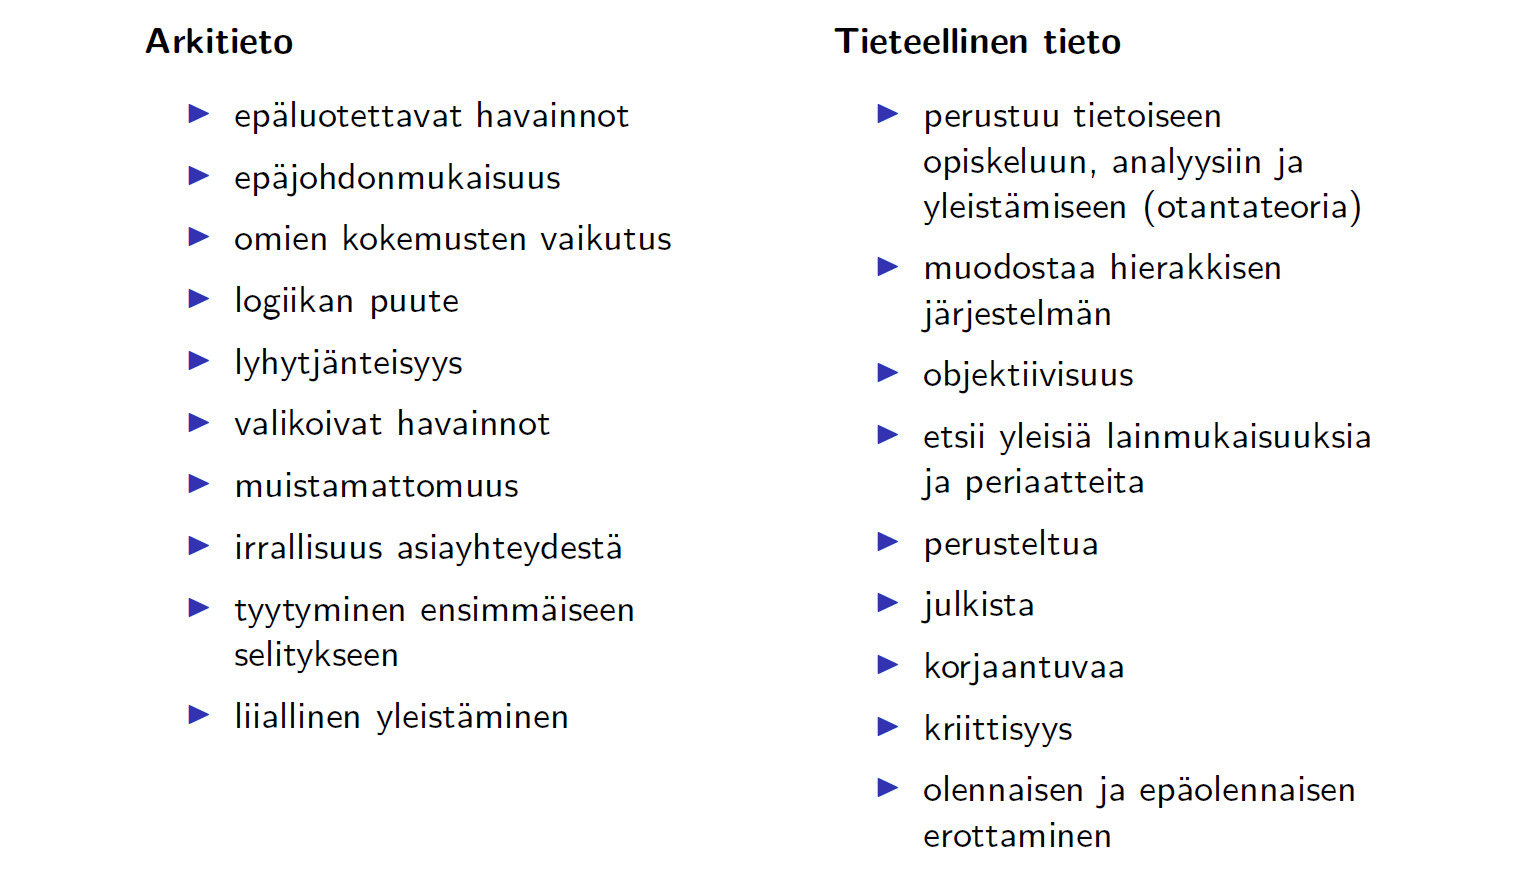
\includegraphics[width=1\linewidth]{images/Arkitieto-tieteellinentieto} 

}

\caption{Arkitieto ja tieteellinen tieto}\label{fig:arki}
\end{figure}

\hypertarget{alaluku22}{%
\section{Tieteellinen menetelmä}\label{alaluku22}}

\begin{itemize}
\tightlist
\item
  Milloin tutkimus sitten on tieteellistä? Tiede on tiedonhankintaa, jossa käytetään erityistä, mahdollisesti tilanteesta (sovelluksesta) riippuvaa, tieteellistä \textbf{menetelmää} eli \textbf{metodia}.
\end{itemize}

\begin{defblock}{}

\textbf{Tieteellinen menetelmä}: Tieteellinen menetelmä on kullakin tieteen alalla vallitseva, ajan myötä kehittynyt ja nykyisten paradigmojen mukainen menettelytapa, jolla uutta tietoa tuotetaan ja vanhaa, mutta epävarmaa tietoa vahvistetaan. Se ei ole selkeä työvaiheiden luettelo tai menetelmähakemisto, vaan yleisesti hyväksytty ja hyväksi todettu tapa pyrkiä totuuteen erilaisten tutkimusongelmien ratkomisessa. Hyvälle tieteelliselle menetelmälle voidaan lukea seuraavia kriteerejä.

\begin{itemize}
\tightlist
\item
  \textbf{Objektiivisuus ja loogisuus}

  \begin{itemize}
  \tightlist
  \item
    Tutkimuskohteen ominaisuudet ovat tutkijan mielipiteistä riippumattomia.
  \item
    Tieteellinen tieto tutkimuskohteesta syntyy tutkijan ja tutkimuskohteen vuorovaikutuksen tuloksena.
  \item
    Tiedon lähteenä on tutkimuskohteesta saatava kokemus.
  \item
    Tutkimuskohteesta voidaan saada totuudellista tietoa, jonka laadusta myös tutkijayhteisö voi olla yhtä mieltä.
  \end{itemize}
\item
  \textbf{Kriittisyys}

  \begin{itemize}
  \tightlist
  \item
    Ilmenee niinä vaatimuksina, joita \textbf{hypoteesin} asettamiselle, testaamiselle ja hyväksymiselle on asetettu.
  \item
    Tieteellisten hypoteesien tulee olla intersubjektiivisesti testattavissa eli niillä täytyy olla yhdessä sopivien lisäoletusten kanssa sellaisia seurauksia, joiden totuus tai virheellisyys voidaan julkisesti tarkistaa.
  \end{itemize}
\item
  \textbf{Autonomisuus}

  \begin{itemize}
  \tightlist
  \item
    Tieteen tulosten arvioiminen on (tiukasti ottaen) tieteellisen yhteisön oma asia, johon tieteen ulkopuolella olevat ryhmät eivät saa vaikuttaa.
  \item
    Ei ole hyväksyttävää vedota siihen, että väitteen totuus olisi toivottavaa tai epätoivottavaa esimerkiksi poliittisista, uskonnollisista tai moraalisista syistä.
  \end{itemize}
\item
  \textbf{Edistyvyys}

  \begin{itemize}
  \tightlist
  \item
    Tieteen edistyminen merkitsee kasvun eli tulosten määrällisen lisääntymisen ohella sitä, että virheellisiä hypoteeseja tai teorioita korvataan uusilla tuloksilla, jotka ovat tosia tai ainakin vähemmän virheellisiä kuin aikaisemmat.
  \end{itemize}
\item
  \textbf{Toistettavuus ja yleistettävyys}

  \begin{itemize}
  \tightlist
  \item
    Tieteen tulokset tulee olla muiden tutkijoiden toistettavissa eli replikoitavissa. Toistettavuudelle (paikoin myös uusittavuudelle, joskin merkitys vaihtelee) on erilaisia määritelmiä.
  \end{itemize}
\end{itemize}

\end{defblock}

\begin{itemize}
\tightlist
\item
  Tarkastellaan lähemmin erästä määritelmää erilaisille toistettavuuden lajeille. Esittelemme tässä Hamermeshin (2007)\footnote{Hamermesh, D. S. (2007). Replication in economics. \emph{Canadian Journal of Economics/Revue canadienne d' ́economique} 40 (3), 715--733.} esittämän erilaisten replikointien jaottelun:

  \begin{itemize}
  \tightlist
  \item
    \textbf{Puhdas replikointi}: toinen tutkija, käyttäen täysin samaa tutkimusaineistoa ja samaa tilastollista menetelmää kuin alkuperäisessä tutkimuksessa, saa täsmälleen samat tutkimustulokset.
  \item
    \textbf{Tilastollinen replikointi}: toinen tutkija, käyttäen eri tutkimusaineistoa (otosta), joka on kuitenkin poimittu samasta populaatiosta (ks. Luku \ref{luku5}), mutta samaa menetelmää, saa vastaavanlaisia tuloksia, jotka vahvistavat alkuperäisen tutkimuksen perustulokset.
  \item
    \textbf{Tieteellinen replikointi}: toinen tutkija, käyttäen samoja asioita mittaavaa tutkimusaineistoa, joka on kuitenkin kerätty eri populaatiosta, ja käyttäen samankaltaista, mutta ei identtistä menetelmää, saa vastaavanlaisia tuloksia, jotka vahvistavat alkuperäisen tutkimuksen perustulokset.
  \end{itemize}
\end{itemize}

\hfill\break
\hfill\break

\begin{itemize}
\tightlist
\item
  Teorioiden sisältämiä väitteitä voidaan muotoilla tieteellisiksi malleiksi, joihin voidaan liittää hypoteeseja, joita testataan tieteellisin menetelmin käyttäen ilmiö(i)stä mitattua havaintoaineistoa.

  \begin{itemize}
  \tightlist
  \item
    Tieteelliset mallit ovat yksinkertaistuksia reaalimaailmasta ja ne kuvaavat tutkimuksen aihetta jostain näkökulmasta tarkasteltavana systeeminä.
  \item
    Mallit hyödyntävät matemaattista esitystapaa, sillä se tarjoaa formaalin ja objektiivisen tutkimusaiheen kuvauksen sekä mahdollistaa siihen liittyvän loogisen päättelyn havaitun, empiirisen aineiston pohjalta.
  \item
    Tilastolliset mallit ovat käytännössä tieteellisten mallien formaaleja matemaattisia esityksiä, jotka lisäksi mahdollistavat mallia koskevan tilastollisen päättelyn esimerkiksi hypoteesien ja niiden
    testaamisen avulla. Päättely perustuu tilastotieteen teoriaan, joka mahdollistaa päättelyn epävarman ja satunnaisen aineiston tapauksissa.
  \item
    Hypoteesien asettamisen voidaan ajatella tutkittavaa ilmiötä koskeviksi ennusteiksi, joita verrataan havaittuun aineistoon. Mikäli havaittu aineisto ei sovi testattavaan teoriaan tai siihen liittyviin hypoteeseihin, voidaan (hieman yksinkertaistaen) teoriaa kehittää paremmaksi. Tämä vuoropuhelu vie tiedettä eteenpäin ja tuottaa lisää tutkittua tietoa ympäröivästä maailmasta.
  \end{itemize}
\item
  Hypoteesien testaaminen on yhtäältä tieteellisten teorioiden kehittämisen ja vahvistamisen ja toisaalta kritiikin keskiössä.

  \begin{itemize}
  \tightlist
  \item
    Metodologinen pluralismi: Kaikkia menetelmiä voi soveltaa hyvin tai huonosti, mutta niitä voi käyttää myös luovasti väärin.
  \end{itemize}
\end{itemize}

\hypertarget{alaluku23}{%
\section{Tilastojen yleisestä roolista yhteiskunnassa}\label{alaluku23}}

\begin{itemize}
\tightlist
\item
  Ihminen ei voi toimia maailmassa järkevästi, ellei hän pysty muodostamaan oikeata kuvaa maailmasta ja sen tilasta. Nykyaikana oikeaa kuvaa varten tarvitaan maailmaa ja sen tilaa merkityksellisesti ja oikein kuvaavia, ajantasaisia \textbf{(tilasto)tietoja}.\\
  \strut \\
\item
  Yhteiskunnan kaikilla sektoreilla toiminnan seuranta, päätöksenteko ja ennakointi perustuvat eri sektoreita kuvaaviin \textbf{(tilasto)tietoihin} ja niiden analysoinnissa käytettäviin \textbf{tilastollisiin menetelmiin}.

  \begin{itemize}
  \tightlist
  \item
    Oikein todellisuutta kuvaavat, ajantasaiset (tilasto)tiedot ovat välttämättömiä modernin yhteiskunnan toiminnalle.
  \item
    Esimerkiksi päätöksenteko sekä julkisella että yksityisellä sektorilla (elinkeinoelämässä) perustuu pitkälti yhteiskuntaa ja elinkeinoelämää kuvaaviin (tilasto)tietoihin ja tilastollisten menetelmien tuottamiin tuloksiin sekä niiden perusteella tehtäviin päätöksiin.

    \begin{itemize}
    \tightlist
    \item
      Esimerkkejä ovat tietyt konkreettiset (talous)poliittiset toimenpiteet (talous)tilastojen perusteella. Lisäksi tuotantoprosessien ohjaus ja laadunvalvonta teollisuudessa sekä markkinatutkimus kaupan alalla perustuvat tilastollisiin menetelmiin.
    \end{itemize}
  \item
    (Tilasto)tietojen saatavuutta voidaan pitää jopa toimivan demokratian edellytyksenä.\\
    \strut \\
  \end{itemize}
\item
  Koska todellisuutta kuvaaviin (tilasto)tietoihin sisältyy (lähes) aina \textbf{epävarmuutta} ja \textbf{satunnaisuutta}, tilastotiede ja tilastolliset menetelmät luovat perustan tilastojen tuotannolle, jalostukselle ja analysoinnille.

  \begin{itemize}
  \tightlist
  \item
    Niinpä tilastojen tuotannon, jalostuksen ja analysoinnin menetelmien kehittäminen on keskeinen osa tilastotieteen tehtäväkenttää.
  \item
    Samoin tilastotieteen menetelmien ymmärtämisellä on keskeinen rooli tietoyhteiskunnassa toimimisessa ja vaikuttamisessa.\\
    \strut \\
  \end{itemize}
\end{itemize}

\begin{eblock}{}

\textbf{Esimerkki (väite)}: Naiset puhuvat enemmän kuin miehet.

\begin{itemize}
\tightlist
\item
  Lähtökohta väitteen (hypoteesin) tutkimiseen:

  \begin{itemize}
  \tightlist
  \item
    Uskomus on väärä kunnes toisin todistetaan.
  \item
    Lähdetään liikkeelle olettamuksesta, että miehet ja naiset puhuvat yhtä paljon.
  \item
    Olettamuksen tueksi tai kumoamiseksi täytyy kerätä todistusaineistoa.
  \item
    Jotta tutkimukseen saataisiin täysin varma vastaus, kaikki miesten ja naisten puheet ihmiskunnan olemassa olon ajalta pitäisi pystyä laskemaan = mahdotonta.
  \end{itemize}
\item
  Mitä siis tehdä?

  \begin{itemize}
  \tightlist
  \item
    Täytyy tyytyä tutkimaan osajoukkoja miehistä ja naisista (otos), mihin tarvitaan \textbf{otantamenetelmiä} (käsitellään tarkemmin myöhemmin luvussa \ref{luku5}).
  \item
    Arvotaan satunnaisesti tutkimushenkilöitä miesten ja naisten joukosta ja mitataan kuinka paljon he puhuvat.
  \item
    Satunnaisuus tärkeää, sillä jos valikoitaisiin tarkoituksella puheliaita tai vähäsanaisia tutkimushenkilöitä, tulokset vääristyisivät.
  \end{itemize}
\item
  Jokaiseen mittaukseen liittyy virhe.

  \begin{itemize}
  \tightlist
  \item
    Täysin satunnainenkaan otos ei edusta täydellisesti koko väestöä. Joukkoon saattaa valikoitua puhtaasti sattumaltakin poikkeuksellisen puheliaita tai harvasanaisia naisia tai miehiä.
  \item
    Millaisia sekoittavia tekijöitä tulee mieleen? Mitkä seikat voisivat vaikuttaa tutkittavaan asiaan?
  \item
    Otoskoolla, eli sillä kuinka monta tutkimishenkilöä tutkitaan, on keskeinen rooli tutkimuksen luotettavuudelle. Mitä suurempi otos, sitä pienemmäksi sattuman osuus käy ja vastaavasti mitä pienempi otos, sitä suurempi on yksittäisten sattumien vaikutus.

    \begin{itemize}
    \tightlist
    \item
      Tilastolliset mallit turvautuvat todennäköisyyksiin erottaakseen sattuman vaikutuksen: kun aineisto on kerätty, halutaan tietää kuinka todennäkoistä on, että uskomus pitää paikkaansa.
    \end{itemize}
  \end{itemize}
\item
  Palataan takaisin esimerkkiimme: Yleisen uskomuksen mukaan naiset puhuvat enemmän kuin miehet.

  \begin{itemize}
  \tightlist
  \item
    Tutkimuksen mukaan miehet vaikuttavat kuitenkin puhuvan yhtä paljon kuin naisetkin.
  \item
    Laajemmat tutkimukset osoittavat, että \textbf{tilanteella} on puheen määrään paljon suurempi vaikutus kuin sukupuolella.
  \end{itemize}
\item
  Kiitos tilastotieteen, väärä uskomus on korvautunut tiedolla!
\end{itemize}

\end{eblock}

\begin{figure}

{\centering 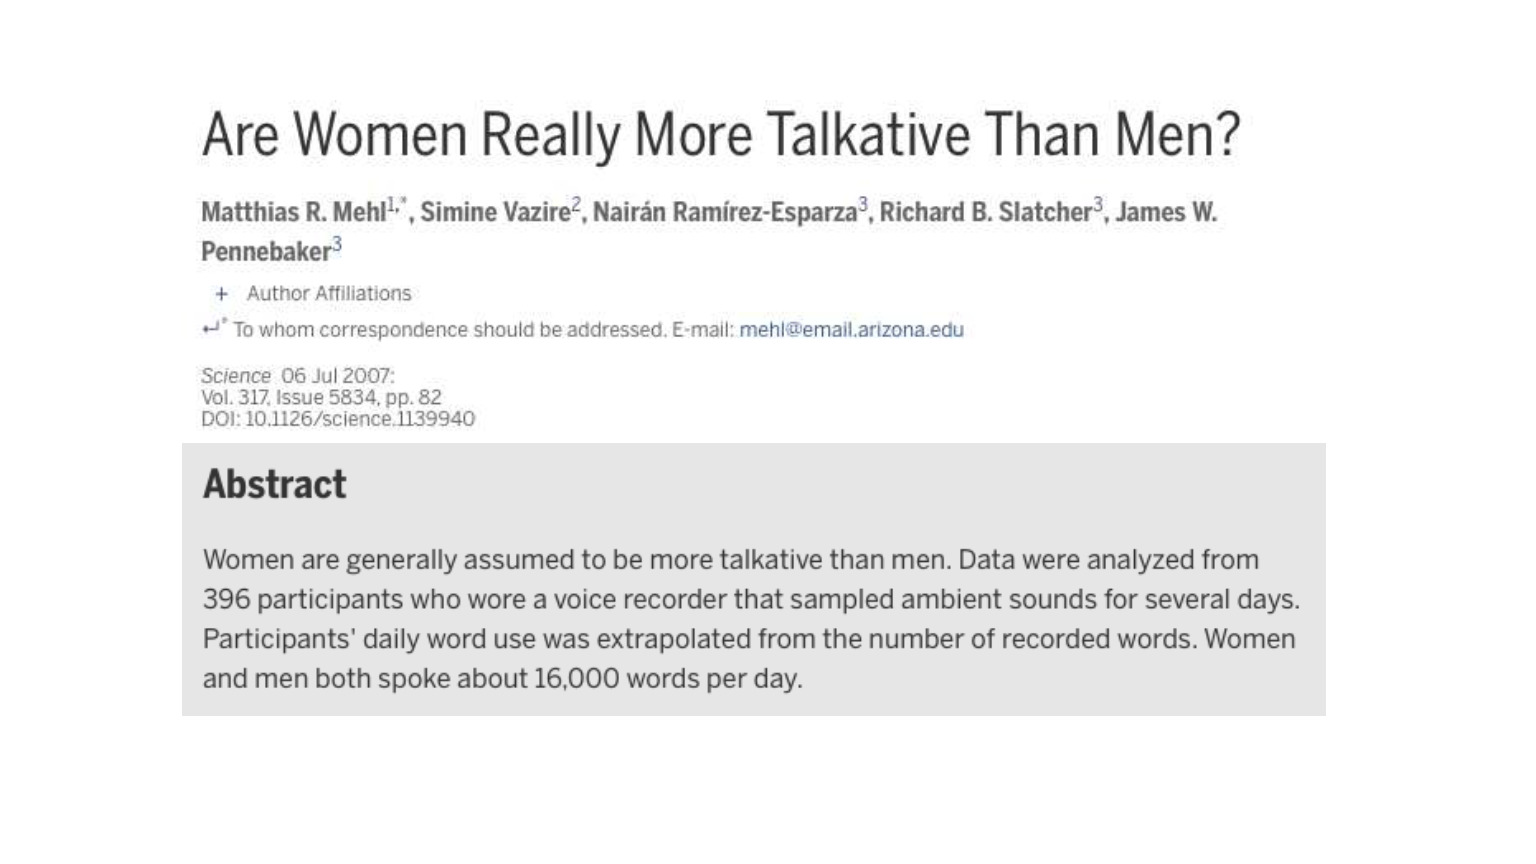
\includegraphics[width=1\linewidth]{images/Are-women-really-more-talkative} 

}

\caption{Are women really more talkative than men?}\label{fig:talkative}
\end{figure}

\hypertarget{alaluku24}{%
\section{Mitä on tutkimus?}\label{alaluku24}}

\begin{itemize}
\tightlist
\item
  Tiede tavoittelee tietoa, mutta mistä?

  \begin{itemize}
  \tightlist
  \item
    Jokaisen tutkimuksen lähtökohtana on (tai ainakin pitäisi useimmiten olla) tiedollisen uteliaisuuden, käytännön tarpeiden tai teorian kehittämispyrkimyksen herättämä ongelma, johon tutkimuksen avulla etsitään vastausta. Tutkimus yrittää käsittää sekä tulkitun ilmiön, että sen tajunnassa synnyttämät spontaanit mielikuvat tai arkipäivän tiedot.
  \item
    Tutkimus siis pyrkii löytämään täysin uutta tietoa, varmentamaan (mahd. aiempien tutkimusten myötä) syntyneitä vallitsevia mutta epävarmoja käsityksiä sekä tarkistamaan vakiintuneen tiedon paikkansapitävyyttä.
  \item
    Valtaosa tieteestä asemoituu kahden viimeisen kohdan alaisuuteen vaikka tieteen popularisoinnissa (mm. median toimesta) usein keskitytäänkin uusiin tiedemaailmaa ja joskus ``käytännön'' elämää järisyttäviin löydöksiin, jotka tosin voivat olla hyvin epävarmoja!
  \item
    Lisää tieteen popularisoinnista jaksossa \ref{alaluku46}.\\
    \strut \\
  \end{itemize}
\item
  Millaisia kysymyksiä \textbf{tutkimuksessa} asetetaan (voidaan asettaa)?

  \begin{itemize}
  \tightlist
  \item
    \textbf{Kuvaus}: Kuinka suuri on yli 65-vuotiaiden osuus Suomen väestöstä?
  \item
    \textbf{Riippuvuuden kuvaus}: Ovatko paljon mainostavat yritykset kannattavampia kuin vähän mainostavat?
  \item
    Kuvattujen ilmiöiden \textbf{selittäminen} ja \textbf{ymmärtäminen}. Miksi vanhempien sosioekonominen asema vaikuttaa ekonomien työhönsijoittumiseen? Tämän tutkimuskysymyksen tapauksessa pyrkimys on lähinnä selittää (ymmärtää) ilmiötä.
  \item
    \textbf{Ennustaminen}: Jos kansantulon kasvu pienenee x\%, työttömyyden ennustetaan kasvavan y tuhannella.
  \item
    Kohdetta kuvaavien käsitteiden ja teorioiden rakentaminen, teorioiden ansioiden ja puutteiden arviointi.
  \end{itemize}
\item
  Myöhemmin materiaalissa (luvussa \ref{luku11}) keskustellaan vielä tarkemmin miten tilastotieteessä ilmiön ymmmärtäminen (selittäminen) ja ennustaminen eroavat toisistaan.\\
  \strut \\
\item
  \textbf{Tutkimuksen rajat?} Onko niitä?

  \begin{itemize}
  \tightlist
  \item
    Tutkimus antaa aina vajavaisen kuvan tutkimuskohteesta.

    \begin{itemize}
    \tightlist
    \item
      Kehittynytkin tieteellinen teoria tai malli on aina reaalimaailman yksinkertaistus: tutkimus on aina alisteinen käytetylle menetelmälle ja sen oletuksille!
    \end{itemize}
  \item
    Ymmärtämiseen tarvittava havaintomaailman hahmotus (saattaa) tuottaa ideologisesti ja historiallisesti sitoutuneita yksinkertaistavia sekä luonteeltaan usein hyvin teoreettisia abstraktioita.

    \begin{itemize}
    \tightlist
    \item
      Alakohtainen substanssitietous sekä sen vahvuuksien ja puutteiden sekä historiallisen ja ideologisen kontekstin tiedostaminen on ensiarvoisen tärkeää kaikessa tutkimuksessa!
    \end{itemize}
  \item
    Joka tapauksessa täyteen neutraaliuteen ja objektiivisuuteen on mahdotonta päästä. Tästä huolimatta on hyvä ja tärkeää pystyä tunnistamaan tämä haaste.
  \item
    Tutkimusta voi tehdä joistakin arvolähtökohdista, mutta sen tulisi olla näkyvää. Omien arvojen mahdollisimman selvä eksplikointi on yksi keino, jolla voi yrittää vähentää piiloarvojen vaikutusta tutkimukseen.

    \begin{itemize}
    \tightlist
    \item
      Arvot ilmenevät esimerkiksi tutkimuksessa käytetyissä käsitteissä, jotka harvoin ovat arvovapaita. Useimmat käsitteet voidaan korvata toisilla, joilla on paikoin hyvin erilainen arvosisältö joskin arvottava lataus saattaa myös olla paikoin tarkoituksellista! Joka tapauksessa arvopainotteisten valintojen tunnistaminen on vaikeaa.
    \item
      Toisaalta arvoihin sitoutuminen on väistämätöntä, sillä se on sosiaalisen olemassaolon sivutuote. Yhteiskunnan jäseninä meillä on tuskin mahdollisuuksia (täydellisesti) irroittautua arvoistamme kun pyrimme esim. ammatillisiin päämääriin.

      \begin{itemize}
      \tightlist
      \item
        Myös päinvastainen ongelma olemassa: Tutkimusta arvioidaan siihen perustellusti tai perusteettomasti kiinnitettyjen arvonäkökohtien mukaan!
      \end{itemize}
    \end{itemize}
  \end{itemize}
\end{itemize}

\hfill\break
\hfill\break

\begin{itemize}
\tightlist
\item
  Tutkimukseen kuuluu olennaisesti myös oman tutkimustyön kuvaaminen, ts. kertomus siitä, miten esitettyihin tuloksiin on päästy.

  \begin{itemize}
  \tightlist
  \item
    Tämän myötä tieteelliselle ajattelulle on ominaista automaattinen \textbf{itsensä korjaaminen}.
  \item
    Tutkimuskysymys, valitut menetelmät, käytetty aineisto ja tehdyt johtopäätökset perataan auki tutkimusartikkelissa/raportissa, joka sitten lähetetään \textbf{vertaisarvioitavaksi} tietelliseen julkaisuun, jossa muut alan asiantuntijat arvioivat sen ja päättävät hyväksytäänkö se julkaistavaksi.
  \end{itemize}
\item
  \textbf{Vertaisarvioinnissa} yksi tai useampi, tehdystä tutkimuksesta riippumaton, saman alan tutkija lukee ja tarkastaa tehdyn tutkimusartikkelin, arvioi sitä ja suosittaa tietellisen julkaisun arvioinnista vastaavalle päätoimittajalle (editorille) kyseisen artikkelin hyväksymistä tai hylkäämistä.

  \begin{itemize}
  \tightlist
  \item
    Vertaisarviointi ei aina takaa sitä, että julkaistu tutkimus olisi virheetön ja erinomaisesti tehty, vaan myös väärää tietoa pääsee välillä vertaisarviointiprosessin läpi.
  \item
    Tämä ei kuitenkaan poista tieteellisen prosessin luotettavuutta, sillä uusi tieto varmentuu vasta usean samaa tutkimuskysymystä tutkineen ja vastaavat tulokset saaneen tutkimuksen myötä. Toisin sanoen, tieteellisen prosessin voidaan ajatella konvergoituvan totuuteen, vaikka yksittäisiä virhearviointeja sattuisikin.\\
  \end{itemize}
\item
  \textbf{Tutkimuksen kieli}

  \begin{itemize}
  \tightlist
  \item
    Tutkimus edellyttää arkikieltä täsmällisempää kommunikaatiota.
  \item
    Ongelmaan liittyvien käsitteiden huolellinen määritteleminen ja erittely on tarpeellista.

    \begin{itemize}
    \tightlist
    \item
      Käsitteiden ja eri aloilla, osin samoista asioista käytettävien, toisistaan eroavien termien systemaattinen määrittely ja jäsentely selkeyttää tiedeyhteisön välistä kommunikointia.\\
    \item
      Eivät korvaa empiiristä tietoa vaan vaikuttavat tiedon järjestymiseen ja sen perusteella tehtäviin päätelmiin.\\
      \strut \\
    \end{itemize}
  \end{itemize}
\end{itemize}

\begin{eblock}{}

\textbf{Esimerkki: Luonnontieteelliset vs.~yhteiskunnalliset sovellutukset}:

\begin{itemize}
\tightlist
\item
  Luonnontieteiden lainalaisuuksia: Monet luonnontieteelliset ilmiöt ovat luonteeltaan varsin pysyviä.

  \begin{itemize}
  \tightlist
  \item
    Voidaan tehdä luotettavasti laajojakin yleistyksiä.
  \item
    Selityksiä voidaan empiirisesti testata.
  \item
    Luotettavia matemaattisia esityksiä voidaan kehittää.
  \end{itemize}
\item
  Yhteiskuntatieteissä (yhteiskuntatieteiden historiallisuuden myötä) erinäisiä lainalaisuuksia ja tyypillisiä piirteitä:

  \begin{itemize}
  \tightlist
  \item
    Usein tutkitaan \textbf{yhteiskunnallisia ilmiöitä}, jotka eivät suurelta osin ole toistettavissa.
  \item
    Vaihtelevat huomattavasti ajan myötä (aiemmin voimassaolleet lainalaisuudet eivät välttämättä ole enää voimassa ja päinvastoin), mikä vaikeuttaa tilastollista analyysiä.
  \item
    Yhteiskunnallisten ilmiöiden mittaaminen?

    \begin{itemize}
    \tightlist
    \item
      Yhteiskunnan rakenne ja toiminta on ehdollinen siinä käytettävän merkitysjärjestelmän suhteen. Kysymys \textbf{mittaamisesta} on asetettava suhteessa tähän käsitejärjestelmään. Joudutaan tekemään erilaisia kompromisseja eksaktisuus- ja systemaattisuusvaatimusten sekä arkikielen monimerkityksellisyyden välillä.
    \end{itemize}
  \end{itemize}
\end{itemize}

\end{eblock}

\hypertarget{alaluku25}{%
\section{Tutkimuksen vaiheet ja tulosten julkaiseminen}\label{alaluku25}}

Tieteellinen tutkimus ja asiantuntijatyö tuottavat valtavan määrän perusteltua, luotettavaa tutkimustietoa. Ks. tarkemmin tieteellisestä julkaisemisesta linkin tapauksessa erityisesti yhteiskuntatieteiden alalla, mutta perusperiaatteet pätevät myös muiden tieteenalojen tapauksessa

\url{https://blogs.uef.fi/tiedonhaku-yhteiskuntatiede/tieteelliset-julkaisut/}\strut \\
\newpage
Vastuullisen tieteen

\url{https://vastuullinentiede.fi/fi/julkaiseminen}

artikkelit tarjoavat tietoa siitä, kuinka tutkittua tietoa tuotetaan, julkaistaan ja arvioidaan luotettavasti ja yhteisesti hyväksytyllä tavalla. Jotta tiede vaikuttaa koko yhteiskunnan hyväksi, toiminnan on oltava vastuullista tutkimuksen jokaisessa vaiheessa.

Helsingin yliopisto tarjoaa lisäksi \href{https://tiedelukutaito.mooc.fi/}{Tiedelukutaidon perusteet -kurssia} MOOC-toteutuksena (Massive Open Online Course). Keskustelethan ennen kurssin käymistä oman alasi koulutussuunnittelijan (tai vastaavan vastuuhenkilön) kanssa siitä, soveltuuko kyseinen kurssi sisällytettäväksi johonkin omaan opintokokonaisuuteesi.

\begin{itemize}
\tightlist
\item
  Julkisuus ja avoimuus tekevät tutkimuksesta tiedettä.
\item
  Tiedeviestintä on tiedeyhteisöjen sisäistä ja ulkoista tiedonvälitystä ja vuorovaikutusta. Tutkimuksesta viestiminen ei ole vain tutkimustuloksista viestimistä. Vastuullinen tiedeviestintä lisää luottamusta tieteelliseen tietoon.
\item
  Tieteellinen julkaiseminen on tutkijoille tärkeä meritoitumisen tapa, ja siksi on tärkeää, että tekijyys määritellään niin, että se palkitsee tutkijat oikeudenmukaisesti.
\end{itemize}

\hypertarget{luvun-2-yhteenveto-keskeisiuxe4-termejuxe4-ja-kokonaisuuksia.}{%
\section{Luvun 2 yhteenveto, keskeisiä termejä ja kokonaisuuksia.}\label{luvun-2-yhteenveto-keskeisiuxe4-termejuxe4-ja-kokonaisuuksia.}}

\begin{itemize}
\tightlist
\item
  Tieteellinen teoria
\item
  Hypoteesi
\item
  Tieteellinen menetelmä ja hyvän tieteellisen menetelmän kriteerit
\item
  Epävarmuus
\item
  Mitä on tutkimus
\end{itemize}

\hypertarget{luku3}{%
\chapter{Tilastotiede tieteenalana}\label{luku3}}

Tässä luvussa hahmottelemme tilastotieteen piirteitä tieteenalana. Käymme läpi tilastotieteelle ominaisia piirteitä, jotka erottavat sen niin lähitieteistä, kuten matematiikasta ja tietojenkäsittelytieteestä, kuin myös sovellusaloista. Usein näkee tilastotieteen typistettävän vain työkaluksi eri sovellusalojen empiiriseen tutkimukseen siitäkin huolimatta että tilastotieteellä on oma rikas teoriapohjansa sekä kiistaton asema omana tieteenalanaan.

Tieteenalan määritteleminen lyhyesti on aina hieman hankalaa. Tästä huolimatta seuraavassa yritämme osaltaan vastata seuraaviin kysymyksiin:

\begin{itemize}
\tightlist
\item
  Mitä tilastotiede on ja mitä se ei ole? Miksi tilastotiede ei ole vain sovellettua matematiikkaa tai matematiikalla höystettyä tietojenkäsittelyä?
\item
  Mihin tilastotiedettä käytetään? Onko tilastotieteellä käyttöä ns. ``akatemian'' eli tutkimusyhteisön ulkopuolella?
\item
  Minkälaista on tyypillinen tilastotiedettä kohtaan esitetty kritiikki?
\end{itemize}

\hypertarget{alaluku31}{%
\section{Lisää tilastotieteen perustermejä}\label{alaluku31}}

Seuraavia tilastotieteen esittelyä ja karakterisointeja ajatellen määritellään seuraavassa lisää tilastotieteellisen tutkimuksen peruskäsitteitä. Näihin käsitteisiin paneudutaan osaltaan tarkemmin mm. luvussa \ref{luku5}.

\begin{itemize}
\tightlist
\item
  Tilastotieteellinen tutkimus tarkastelee reaalimaailman ilmiöitä. Täten tutkimuskohteena on tavallisessa elämässä tavattavia asioita, ihmisiä tai tapahtumia. Tutkimuskohteita kutsutaan \textbf{tilastoyksiköiksi} ja niiden joukkoa kutsutaan \textbf{populaatioksi (perusjoukoksi)}.
\end{itemize}

\begin{eblock}{}

\textbf{Esimerkki: vaalitutkimus}:

\begin{itemize}
\tightlist
\item
  Politiikan tutkimuksen alalla yksi mielenkiintoinen tutkimuskohde on tutkia kuntavaaleissa äänestävien ihmisten tuloja.

  \begin{itemize}
  \tightlist
  \item
    Tällöin jokainen äänioikeuttaan käyttävä muodostaa oman tilastoyksikkönsä.
  \item
    Vastaavasti populaationa (perusjoukkona) (ks. alla) toimii kaikki äänestysikäiset kansalaiset, jotka äänioikeuttaan käyttävät.
  \item
    Pohdi: miksi pelkästään äänioikeuttaan käyttävien tutkiminen saattaisi olla tutkimuksen tulosten luotettavuuden kannalta ongelmallista?
  \end{itemize}
\item
  Toinen tutkimuskysymys voisi käsitellä kuntien välistä äänestysaktiivisuutta.

  \begin{itemize}
  \tightlist
  \item
    Tällöin jokainen kunta muodostaa oman tilastoyksikkönsä ja vastaavasti kaikki Suomen kunnat muodostavat populaation.
  \item
    Kuntien äänestysaktiivisuus saadaan kuitenkin tutkimalla kunnan sisäistä äänestysaktiivisuutta.

    \begin{itemize}
    \tightlist
    \item
      Toisin sanoen, voidaksemme mitata kuntien äänestysaktiivisuutta, tulee ensiksi selvittää kuntien äänestysikäiset kansalaiset ja äänioikeuttaan käyttävät.
    \end{itemize}
  \end{itemize}
\end{itemize}

\end{eblock}

\begin{defblock}{}
\textbf{Populaatio}

Konkreettinen tai hypoteettinen tutkimuskohteiden joukko, joka koostuu kaikista tilastoyksiköistä

\end{defblock}

\begin{itemize}
\tightlist
\item
  Populaation muodostavilta tilastoyksiköiltä tarkastellaan niiden ominaisuuksia, eli \textbf{tilastollisia muuttujia}.

  \begin{itemize}
  \tightlist
  \item
    Edellisissä esimerkeissä nämä olisivat esim. äänestäjien tulot ja kuntien äänestysprosentti.
  \item
    Mielenkiinnon kohteena olevia tilastollisia muuttujia kutsutaan \textbf{tutkimusmuuttujiksi} (tulot ja kuntien äänestysprosentti) ja niiden lisäksi voidaan kerätä lisätietoa eli \textbf{taustamuuttujia} (näitä voisivat olla esimerkiksi asuinpaikka ja kunnan väkiluku).
  \item
    Tilastoyksiköiden tilastollisilla muuttujilla on tietty mahdollisten arvojen joukko, ja näillä arvoilla on jokin \textbf{jakauma} populaatiossa.

    \begin{itemize}
    \tightlist
    \item
      Esimerkiksi tulot voivat määritelmästä riippuen saada minkä tahansa positiivisen arvon mutta äänestysprosentti on luonnollisesti rajattu nollan ja sadan prosentin väliin.
    \end{itemize}
  \end{itemize}
\end{itemize}

\begin{defblock}{}
\textbf{Tilastoyksikkö ja tilastollinen muuttuja}

Populaation muodostavilta tilastoyksiköiltä (populaation alkioilta) tarkastellaan tilastollisia muuttujia, joita voidaan mitata tai havaita.

\end{defblock}

\begin{itemize}
\tightlist
\item
  Kun tarkasteltavien tilastoyksikön tilastollisten muuttujien (numeeriset) arvot havaitaan, kutsutaan näiden arvojen joukkoa \textbf{havainnoksi}
\end{itemize}

\begin{defblock}{}
\textbf{Havainto}

Havainto muodostuu tilastoyksikön tarkasteltavien tilastollisten muuttujien havaitusta arvoista.

\end{defblock}

\begin{itemize}
\tightlist
\item
  Kerättyjen havaintojen joukko muodostaa \textbf{havaintoaineiston}, eli \textbf{datan}.
\end{itemize}

\begin{defblock}{}
\textbf{Havaintoaineisto/data}

Havaintoaineisto, data, on tilastoyksiköiden tilastollisista muuttujista kerätty havaintojen joukko.

\end{defblock}

\textbf{Tiivistettynä}:

\begin{itemize}
\tightlist
\item
  Populaatio koostuu tutkimuksen kohteena olevista tilastoyksiköistä.
\item
  Havaitaan tilastoyksiköistä tutkimuksen kannalta mielenkiintoisia tilastollisten muuttujien numeerisia arvoja.
\item
  Nämä havainnot muodostavat havaintoaineiston, eli datan, jota voidaan käyttää tutkimuksessa ja tutkia \textbf{populaation ominaisuuksia}.
\end{itemize}

\hypertarget{alaluku32}{%
\section{Mitä tilastotiede on ja mitä se ei ole?}\label{alaluku32}}

\begin{itemize}
\tightlist
\item
  Aloitetaan tarkastelemalla erinäisiä \textbf{tilastotieteen ``karakterisointeja''} eri tahojen ja tutkijoiden toimesta:

  \begin{itemize}
  \tightlist
  \item
    \textbf{\emph{Tilastotiede on tietotuotannon teknologiaa}}, \emph{jonka avulla voidaan suorittaa kvantitatiivisten tietojen joukkotuotantoa ja havaintoihin perustuvia tieteellisiä ja käytännöllisiä päätöksiä. Tilastotiede on siis yksikköjen muodostamaan joukkoon liittyvän numeerisen tietoaineiston keräämistä, analysointia ja tulkintaa koskeva tiede} \footnote{\href{https://fi.wikipedia.org/wiki/Leo_T\%C3\%B6rnqvist}{Leo Törnqvistin}, Suomen ensimmäisen tilastotieteen professorin, esittämä luonnehdinta (Vartia, 1989).}.
  \item
    \textbf{\emph{Tilastotiede on yleinen menetelmätiede}}, \emph{jota sovelletaan, jos reaalimaailman ilmiöstä halutaan tehdä johtopäätöksiä ilmiötä kuvaavien kvantitatiivisten tai numeeristen tietojen perusteella sellaisissa tilanteissa, joissa tietoihin liittyy epävarmuutta tai satunnaisuutta} \footnote{Mellin (2005).}.
  \item
    \emph{Vale, emävale, tilasto} \footnote{\href{https://fi.wikipedia.org/wiki/Mark_Twain}{Mark Twain} popularisoi tämän lausahduksen teoksessaan \emph{Chapters from My Autobiography} jo vuonna 1907. Huomionarvoista toki on, että valtaosa ``modernin'' tilastotieteen, jolle nykytilastotiede pohjautuu, teoriakehityksestä on tapahtunut vasta Twainin teoksen julkaisun jälkeen. Esimerkiksi Ronald Fisher, jota pidetään modernin tilastotieteen isänä, julkaisi merkityksellisimmät työnsä vasta 1920- ja 30-lukujen aikana. Tällä lentävällä lausahduksella ei siis ole mitään tekemistä nykyisten tilastollisten menetelmien kanssa.}.
  \item
    \emph{Statistics concerns what can be learned from data} \footnote{(A.C. Davison)}.
  \item
    \emph{``Maalaisjärjen tehostamista''} \footnote{Sund, (2003)}.
  \end{itemize}
\item
  Tilastotiede siis \textbf{kehittää} ja \textbf{soveltaa menetelmiä} ja (tilastollisia) \textbf{malleja}, joiden avulla reaalimaailman ilmiöistä voidaan tehdä johtopäätöksiä ilmiöitä kuvaavien numeeristen tai kvantitatiivisten tietojen perusteella tilanteissa, joissa tietoihin liittyy \textbf{epävarmuutta ja satunnaisuutta}.

  \begin{itemize}
  \tightlist
  \item
    Tilastollisten menetelmien avulla pyritään löytämään reaalimaailman satunnaisia ilmiöitä kuvaavista numeerisista (eli kvantitatiivisista) tiedoista \textbf{systemaattisia piirteitä} joita jalostetaan sellaiseen muotoon, että ilmiöistä voidaan tehdä päätelmiä.

    \begin{itemize}
    \tightlist
    \item
      Vrt. signaalin ja kohinan erottaminen (ks. Silver, 2014)\footnote{Silver, N. (2014). Signaali ja kohina: Miksi monet ennusteet epäonnistuvat mutta jotkin eivät? Terra Cognita. (Suomentanut Kimmo Pietiläinen)}.
    \end{itemize}
  \item
    Tilastolliset mallit perustuvat todennäköisyyslaskentaan ja niillä mallinnetaan reaalielämän ilmiöiden alla piileviä prosesseja tai mekanismeja. Näiden prosessien tuottamia tietoja (aineistoja) tiivistetään usein graafisiksi esityksiksi ja tunnusluvuiksi sekä tilastollisten mallien parametreiksi, joiden pohjalta johtopäätöksiä tehdään.
  \item
    Tässä onnistuakseen tilastollisten menetelmien tuleekin pyrkiä erottelemaan \textbf{sattuma} ja \textbf{systemaattisuus} tarkasteltavissa ilmiöissä tai, tarkemmin, niitä kuvaavissa aineistoissa, jotta johtopäätökset olisivat luotettavia.
  \end{itemize}
\end{itemize}

\hfill\break

\textbf{Voidaan sanoa, että saadakseen tarkemmin selville mitä tilastotiede on, pitää opiskella tilastotiedettä ja sen käyttöä!}

\hfill\break

\textbf{Mitä tilastotiede ei ole}

\begin{itemize}
\tightlist
\item
  \textbf{Tilastotiede ei ole vain tilastojen tuotantoa}

  \begin{itemize}
  \tightlist
  \item
    Vaikka sana \textbf{tilasto} tuo useimmille ensimmäisenä mieleen yhteiskuntaa ja sen toimintaa kuvaavat \textbf{numeeristen tietojen järjestelmälliset kokoelmat}, tilastotiede ei suinkaan ole ainoastaan tilastojen ja niiden tekemisen oppia.

    \begin{itemize}
    \tightlist
    \item
      Tämä siitäkin huolimatta, että niiden menetelmien konstruointi, joilla näitä tilastoja tuotetaan, jalostetaan ja analysoidaan on keskeinen osa tilastotiedettä. Tilastot ovat siis usein tilastotieteen soveltajan tutkimuskohteena ja tilastojen laadinnassa käytetään apuna tilastotieteen menetelmiä.
    \item
      Suomessa \href{https://www.stat.fi/}{Tilastokeskus} toimii virallisena tilastoviranomaisena ja tilastotuottajana. Tätä \textbf{tilastotuotannon} kokonaisuutta nimitetään ajoittain \textbf{tilastotoimeksi}. \textbf{Tilastotieteen käyttöalue on paljon tätä laajempi}.
    \item
      Terminologiaa:

      \begin{itemize}
      \tightlist
      \item
        Tilastoala = Tilastotiede + Tilastotoimi\\
      \item
        Tilastotiede = Teoreettinen tilastotiede + Soveltava tilastotiede\\
      \item
        Tilastotoimi = Tilastojen tuotanto + Tilastojen hyödyntäminen
      \end{itemize}
    \end{itemize}
  \end{itemize}
\item
  Tilastotieteen kannalta mikä tahansa reaalimaailman ilmiötä kuvaava \textbf{numeeristen tai kvantitatiivisten tietojen järjestelmällinen kokoelma} voi muodostaa \textbf{tilastollisen aineiston} ja siten tilastollisen tutkimuksen mahdollisen kohteen.

  \begin{itemize}
  \tightlist
  \item
    Esimerkiksi kaikki \textbf{empiirisen} tai \textbf{kvantitatiivisen} tutkimuksen tutkimus- tai havaintoaineistot ovat tilastotieteen kannalta tilastollisia aineistoja.
  \end{itemize}
\end{itemize}

\hfill\break

\begin{itemize}
\tightlist
\item
  Tilastotiede sijoittuu tieteiden kentässä matematiikan, filosofian ja tietojenkäsittelytieteen rinnalle. Tästä huolimatta se ei kuitenkaan ole yksiselitteisesti minkään näiden osa-alue.

  \begin{itemize}
  \tightlist
  \item
    \textbf{Tilastotiede ei ole matematiikan osa-alue}, sillä tilastotiede lähestyy tieteellistä ongelmanratkaisua eri tavoin:

    \begin{itemize}
    \tightlist
    \item
      Matematiikka on tietyllä tavalla aina eksaktia ja sen tulokset perustuvat formaaliin deduktioon ja loogisiin todistuksiin, johtaen usein ``eksaktiin'' ratkaisuun tai matemaattisesti formaaliin ratkaisun loogiseen esitystapaan.
    \item
      Tilastotiede sen sijaan on aina konteksti- ja aineistopohjaista ja perustuu induktiiviseen päättelyyn. Saadut tulokset ovat aina epävarmoja - koska ne kuvailevat epävarmaa tietoa generoivia prosesseja!

      \begin{itemize}
      \tightlist
      \item
        Tilastotiede on siis hyvä nähdä omana tieteenalanaan matemaattisesta esitystavastaan huolimatta. Eihän esimerkiksi myöskään fysiikkaa (sentään) pidetä matematiikan osa-alueena!
      \end{itemize}
    \end{itemize}
  \item
    \textbf{Tilastotiede ei ole myöskään tietojenkäsittelytieteen osa-alue}, vaikkakin useiden laskennallisten menetelmien ja tehokkaan tietojenkäsittelyn rooli tilastollisissa analyyseissä on jatkuvasti kasvanut.

    \begin{itemize}
    \tightlist
    \item
      Tietojenkäsittelytieteen teoria ei rakennu tilastotieteen tavoin ajatukselle epävarmoista ja satunnaisista reaalimaailman ilmiöistä.
    \end{itemize}
  \end{itemize}
\item
  Vaikka nämä ja jotkin muut alat jakavat tilastotieteen kanssa useita piirteitä ja ominaisuuksia, on tilastotiede kuitenkin siis perustellusti oma tieteenalansa. Tämä erottelun vaikeus jo itsessään todistaa kuinka keskeinen rooli tilastotieteellä on eri aloilla!

  \begin{itemize}
  \tightlist
  \item
    Tilastotiede ei siis kuulu yksiselitteisesti sen lähitieteiden alle, vaan muodostaa oman tieteenalan omine teorioineen ja tieteellisine premisseineen. Käsittelemme myöhemmin tilastotieteen roolia matematiikan ja/tai datatieteiden (``data science'') kokonaisuudessa ja keskustelemme tarkemmin näiden erojen luonteesta.
  \end{itemize}
\end{itemize}

\hfill\break
\hfill\break

\textbf{Mitä tilastotiede (ainakin) on}

\begin{itemize}
\tightlist
\item
  \textbf{Tilastotiede yleisenä menetelmätieteenä}

  \begin{itemize}
  \tightlist
  \item
    Tieteellistä tietoa ympäröivästä maailmasta hankitaan tieteellisillä \textbf{menetelmillä/metodeilla} (ks. tieteellisen menetelmän kriteerit luku \ref{luku2})), joiden avulla tutkitaan jotain ilmiötä tai sen generoimaa kvantitatiivista mutta epävarmaa tietoa sisältävää aineistoa.
  \item
    Tilastotieteessä kehitetyt ja kehitettävät menetelmät antavat tutkijoille yhtenevät ja tiedeyhteisön hyväksymät raamit, jotka mahdollistavat (tilastollisen) päättelyn ja päätöksenteon epävarman tiedon vallitessa. Näin voidaan uskottavasti ja luotettavasti tiivistää tietoa, jota erilaiset aineistot sisältävät, perustaa johtopäätöksiä näille tiivistyksille ja saavuttaa uusia tieteellisiä löytöjä.

    \begin{itemize}
    \tightlist
    \item
      Tilastotieteen menetelmien käyttö ja soveltaminen onkin siis aina alakohtaista. Tästä huolimatta tilastollisia menetelmiä sovelletaan aina johonkin \textbf{aineistoon}!
    \end{itemize}
  \item
    Tilastotieteen nähdäänkin usein kuuluvan ns. \textbf{menetelmätieteisiin}, joissa mm.:

    \begin{itemize}
    \tightlist
    \item
      Kehitetään työkaluja muiden tieteiden tutkimusongelmien ratkaisuksi
    \item
      On myös oma sovelluksista vapaa teorianmuodostuksensa
    \end{itemize}
  \item
    Menetelmäkehityksen näkökulma tilastotieteeseen: \emph{tilastotiede kehittää matemaattisia} \textbf{\emph{malleja}} \emph{satunnaisilmiöitä kuvaavia kvantitatiivisia tietoja generoiville prosesseille.} Koska tietoihin liittyy \textbf{epävarmuutta} tai \textbf{satunnaisuutta}, \textbf{tilastolliset mallit} perustuvat \textbf{todennäköisyyslaskentaan}.

    \begin{itemize}
    \tightlist
    \item
      Juuri sattuman ja epävarmuuden huomioiminen tutkimusasetelmissa erottaa tilastotieteen muista menetelmätieteistä!
    \end{itemize}
  \end{itemize}
\item
  Tilastollisia menetelmiä voidaan soveltaa tietojen keruun, jalostuksen ja analysoinnin jokaisessa vaiheessa. Päämääränä on jalostaa tiedot muotoon, joka mahdollistaa tutkittavaa reaalimaailman ilmiötä koskevien johtopäätösten tekemisen käytettyjen menetelmien pohjalta, eli ns. \textbf{tilastollisen päättelyn}.

  \begin{itemize}
  \tightlist
  \item
    Tutkimuksessa on pystyttävä valitsemaan ja käyttämään menetelmiä, jotka antavat aineistosta vastauksia haluttuihin kysymyksiin. Tämä vaatii yhtä lailla sovellusalakohtaista osaamista (ns. \textbf{substanssiosaamista}) kuin myös kattavaa \textbf{menetelmäosaamista}.
  \end{itemize}
\end{itemize}

\hfill\break
\hfill\break

\begin{itemize}
\tightlist
\item
  Tilastotieteessä lähtökohtana ja ratkaisevassa asemassa on siis aina jonkin satunnaisilmiön generoima \textbf{aineisto}, josta haluamme oppia tai tietää lisää, kenties voidaksemme tehdä suuria yhteiskunnallisia päätöksiä sen pohjalta!

  \begin{itemize}
  \tightlist
  \item
    Tämä aineistokeskeisyys yhtäältä erottaa tilastotieteen rajatieteistään ja toisaalta tuo sen lähemmäksi niitä ja sovellusalojaan.
  \item
    Aineistoa analysoidaan, kuvaillaan ja mallinnetaan tilastollisin menetelmin, joiden kehittäminen on keskeinen osa tilastotiedettä.
  \item
    Pelkkä menetelmien kehittäminen kuuluu pitkälti matemaattisen/teoreettisen tilastotieteen osa-alueelle.
  \item
    Pelkkä ainestoon keskittyminen ja (mekaaninen) analysointi voi sen sijaan olla joissain tilanteissa pitkälti tietojenkäsittelyä.
  \end{itemize}
\item
  \textbf{Tilastollinen ``mallintaminen''} löytyykin näiden välistä ja se sisältää eri alojen sovelluksista kumpuavan tarpeen uusien menetelmien kehittämiseen.

  \begin{itemize}
  \tightlist
  \item
    Tämä vuoropuhelu muodostaa tilastotieteelle luonnollisen ``takaisinkytkennän'' teoreettisen ja soveltavan puolen välillä: uudet teoreettiset menetelmät vastaavat soveltavan tilastotieteen ongelmiin mutta herättävät aina uusia kysymyksiä, jotka palautuvat taas teoreettisen tilastotieteilijän pöydälle!
  \item
    Luonnollisesti valtaosa tilastotieteilijöistä ja lähitieteiden harrastajista asettuvat näiden äärimmäisten luonnehdintojen välimaastoon eikä tarkkaa luokittelua ole sinänsä tarpeen tehdä ja korostaa.
  \item
    Joka tapauksessa tilastotieteen kehityksen keskiössä ovat aina sovellusalakohtaiset ongelmat, joista useat palautuvat yleisemmälle tasolle teoreettisen tilastotieteen kehityspolkuihin.
  \end{itemize}
\end{itemize}

\hypertarget{alaluku33}{%
\section{Tilastotieteen suhde lähitieteisiin}\label{alaluku33}}

\begin{itemize}
\tightlist
\item
  Kuvio \ref{fig:datasc}\footnote{Kuvan lähde: \href{https://duchesnay.github.io/pystatsml/introduction/machine_learning.html}{Duchesnay (2020)}} tarjoaa karkean yleistyksen tietojenkäsittelytieteen (Computer Science) ja sovellusalan (Application domain) sekä tilastotieteen (Statistics) ja matematiikan (Mathematics) välisistä yhteyksistä. On selvää että tilastotieteellä on paljon päällekäisyyksiä lähitieteidensä kanssa ja joskus näkeekin (huolimatta edellä tehdyistä huomioista) että tilastotiede niputetaan yhteen matematiikan tai tietojenkäsittelytieteen kanssa.
\end{itemize}

\begin{figure}

{\centering 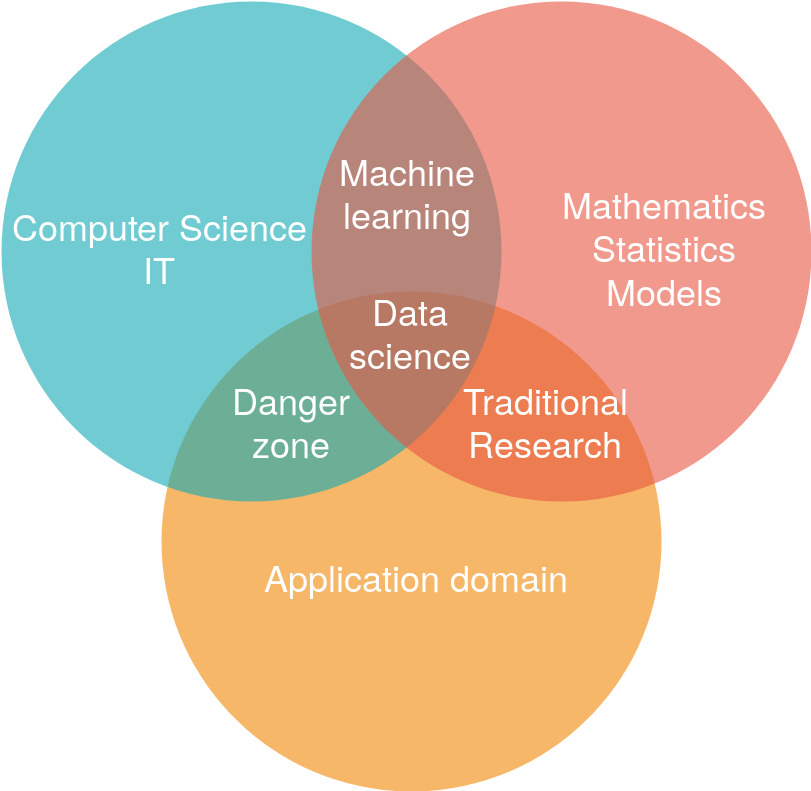
\includegraphics[width=1\linewidth]{images/data_science} 

}

\caption{Tilastotieteen ja rajatieteiden yhteyksiä kuvaava Venn-diagrammi. (Duchesnay, 2020)}\label{fig:datasc}
\end{figure}

\begin{itemize}
\tightlist
\item
  Yritetään siis vielä hahmotella tilastotieteen suhdetta sitä lähimpänä olevaan (soveltavaan) matematiikkaan.

  \begin{itemize}
  \tightlist
  \item
    Tilastotieteessä olennaisen otantateorian (Luku \ref{luku5}) voisi ajatella olevan matemaattisesti määritelty teoria, jossa myös on aineiston käsite, mutta se ei tee siitä vielä varsinaisesti tilastotiedettä.
  \item
    Matematiikassa kuvataan ongelma ja esitetään se teorian muodossa, eli malli on \emph{``parametreista havaintoihin''}.
  \item
    Tilastotieteessä ongelma on käänteinen, edetään \emph{``havainnoista parametreihin''}, mutta ongelman matemaattinen kuvaus vaaditaan ensin.
  \item
    Tilastotiede esittää menetelmiä ja käsitteitä tämän käänteisen ongelman ratkaisemiseen.

    \begin{itemize}
    \tightlist
    \item
      Karkeasti erotellen tilastotieteessä käsiteltävät ongelmat lähtevät aina havainnoista eli aineistosta ja matematiikassa suunta on teoriasta aineistoon.
    \item
      Voidaankin siis sanoa, että tilastotieteen erottaa puhtaasta matematiikasta se, että siinä tutkitaan menetelmiä eli metodeja, jotka mahdollistavat päättelyn/tiedon hankinnan puutteellisesta tai epävarmasta tiedosta.
    \end{itemize}
  \end{itemize}
\item
  Ilmiöiden kuvaamiseen ja käyttäytymisen ennakoimiseen käytetään usein \textbf{mallia}. Mallit (matemaattiset/tilastolliset mallit) voidaan jakaa \textbf{deterministisiin} ja \textbf{stokastisiin} malleihin.

  \begin{itemize}
  \tightlist
  \item
    Deterministisen mallin tapauksessa, tiettyjen alkuehtojen (alkuarvojen) vallitessa voidaan määrittää tarkasteltavan ilmiön lopputulos. Esimerkkejä ovat esim. monet fysiikan lait.
  \item
    Stokastiset mallit perustuvat todennäköisyyslaskentaan. Stokastisia malleja käytetään kun alkuehtojen perusteella ei voida varmasti määrittää tarkasteltavan ilmiön lopputulosta. Tällöin eri vaihtoehtoihin liittyvät tietyt esiintymistodennäköisyydet. Esimerkkejä ovat esim. kolikonheitto tai sään ennustaminen.
  \item
    Kun jotain ilmiötä kuvataan stokastisen mallin avulla, voidaan käyttää (joudutaan käyttämään) tilastollisia menetelmiä. Vaikka käytännössä laskenta hoidetaan tietokoneohjelmien avulla, meidän tilastotieteen tutkijoina ja käyttäjinä on huolehdittava tutkimusprosessin onnistuneesta toteutuksesta muilta osin.
  \end{itemize}
\end{itemize}

\hfill\break
\hfill\break

\begin{itemize}
\tightlist
\item
  Tilastotiede ei myöskään ole puhtaasti tietojenkäsittelyä, vaikka tilastotiede onkin luonteeltaan aineistopohjaista ja aineistojen sisältämää tietoa on käsitelty osin samoin kuin tietojenkäsittelyssä siitä asti kun se on ollut mahdollista (tietokoneen keksimisen myötä).

  \begin{itemize}
  \tightlist
  \item
    Tilastotieteen ja tietojenkäsittelytieteen ero on lähitieteistä selvin: tilastotieteellä on ``mekaanisesta'' tai teoreettisesta tietojenkäsittelystä selkeästi erillinen ja oma teoriapohjansa.

    \begin{itemize}
    \tightlist
    \item
      Siinä missä tilastotieteen teoria perustuu aineiston stokastiselle mallintamiselle, tietojenkäsittely on enemmänkin algoritmista ajattelua, missä aineistolla on ratkaisevalla tavalla erilainen rooli.
    \end{itemize}
  \item
    Lisäksi suomen kielessä tietojenkäsittely ymmärretään laajemmassa mielessä ohjelmoitavissa olevaksi automatisoimiseksi, jota tilastotiede ei perusolemukseltaan suinkaan ole.
  \end{itemize}
\end{itemize}

\hfill\break
\hfill\break

\begin{itemize}
\tightlist
\item
  Tarkastellaan seuraavaksi tilastotieteen suhdetta viime vuosien aikana paljon suosiota keränneeseen \textbf{datatieteeseen (data science)} johon voidaan katsoa lukeutuvan mm.

  \begin{itemize}
  \tightlist
  \item
    Tilastotiede ja matematiikka

    \begin{itemize}
    \tightlist
    \item
      Erityisesti tilastollinen data-analytiikka ja satunnaisen aineiston mallintaminen sekä soveltuvat soveltavan matematiikan osa-alueet.
    \end{itemize}
  \item
    Tietojenkäsittely

    \begin{itemize}
    \tightlist
    \item
      Tietoteknologian kehityksen myötä taitavien tietojenkäsitteljöiden kysyntä on kasvanut merkittävästi. Lähes jokaisella alalla kerätään entistä enemmän dataa lähes kaikesta, ja jonkun pitäisi osata myös käsitellä sitä!
    \item
      Datatieteen voidaankin osaltaan katsoa syntyneen tästä elinkeinoelämän tarpeesta asiantuntijoille, jotka osaavat käsitellä suuria tietoaineistoja (dataa) sekä mallintaa niitä hyödyllisellä tavalla.
    \end{itemize}
  \item
    Sovellusala

    \begin{itemize}
    \tightlist
    \item
      Datatiede on luonteeltaan pääosin soveltavaa ja sen alaan lukeutuvia menetelmiä sovelletaan aina johonkin tosielämän ongelmaan. Tästä syystä substanssiosaaminen sovellusalalta on datatieteilijälle erityisen tärkeää ja nykypäivänä datatieteilijän rooli onkin pirstaloitunut yhä enemmän eri sovellusalojen datatieteisiin.
    \item
      Tästä huolimatta datatieteilijöiden käyttämät mallinnusmenetelmät ovat usein varsin samanlaisia, sillä ne pohjautuvat edelleen tilastotieteen ja matematiikan teoriapohjaan. Ilman jälkimmäisten riittävää osaamista, liikutaan datatieteen osalta vaarallisilla vesillä! (Ks. oheinen kuva ja keskustelu alla).\\
    \end{itemize}
  \end{itemize}
\item
  Datatieteellä ei usein nähdä olevan omaa historiallisen tieteellisen prosessin luomaa teoriapohjaa vaan sen voidaan katsoa olevan kokoelma eri alojen tieteellisiä menetelmiä ja tuloksia, jotka voidaan yhdistää tavalla, jonka ``datavallankumous'' (ks. kuva \ref{fig:datarevolution}) mahdollistaa ja jotka ovat keskeisessä roolissa dataintensiivisissä sovellutuksissa.
\end{itemize}

\begin{figure}

{\centering 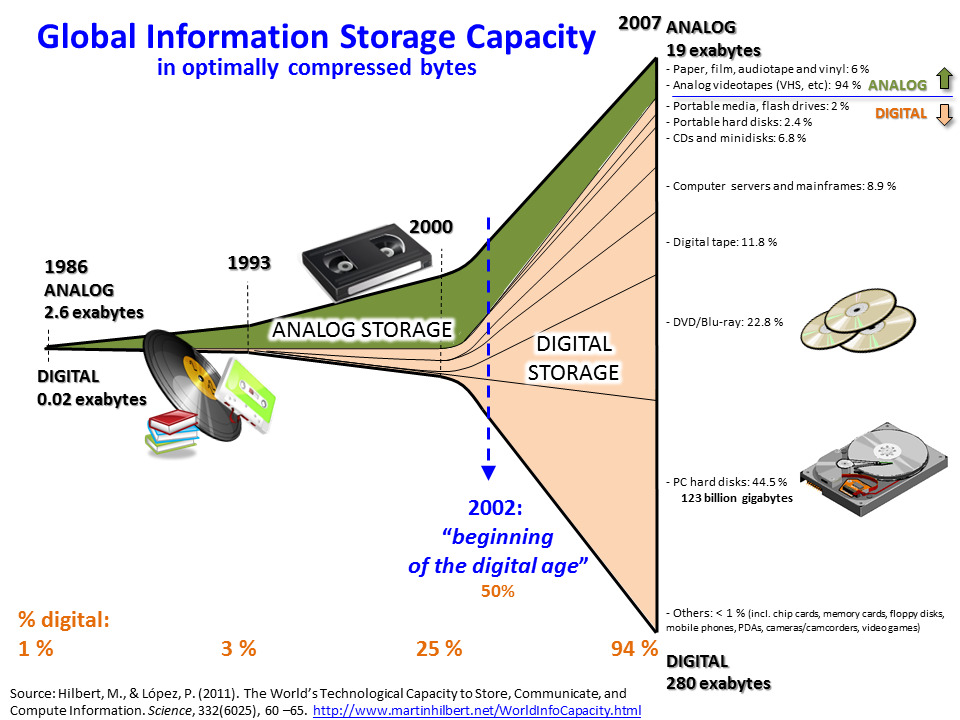
\includegraphics[width=1\linewidth]{images/datarevolution} 

}

\caption{Datavallankumous (Hilbert, M. ja Lopez, P. (2011) The Worlds Technological Capacity to Store, Communicate and Compute Information. Science, 332(6025), 60-65.}\label{fig:datarevolution}
\end{figure}

\begin{itemize}
\tightlist
\item
  ``Danger zone''

  \begin{itemize}
  \tightlist
  \item
    Kuvan \ref{fig:datasc} ``danger zone'' (\href{https://duchesnay.github.io/pystatsml/introduction/machine_learning.html}{Duchesnay, 2020}) kuvaa tilannetta, jossa ilmiöiden/mallien tilastotieteellinen perusta unohdetaan.
  \item
    Tilastotieteen näkökulman ohittava (laiminlyövä) soveltaja ei aina kykene suhtautumaan kriittisesti muodostuvaa ennustemallia, tai ennustetulosta, kohtaan eikä täten päädy parhaisiin mahdollisiin (tarkimpiin) ennustetuloksiin tilanteessa, jossa jokin toinen malli kuvaisi ilmiötä annettua mallia paremmin.
  \item
    Ko. soveltaja ottaa mallin sekä sen antaman ennustetuloksen annettuna, eikä mieti \emph{mistä kyseinen ennustetulos johtuu}. Jotta tarkat ennustetulokset toteutuvat jatkossakin (kun uutta aineistoa, dataa, tulee saataville), on ennustajan oleellista huomioida mitkä tekijät johtivat tarkkaan ennustulokseen.
  \item
    Eri menetelmät sopivat eri sovelluskohteisiin. Tilastotieteilijä osaa useimmiten tunnistaa eri sovelluskohteisiin sopivat menetelmät paremmin kuin tietojenkäsittelijä. Vastaavasti tehokkaan/onnistuneen ohjelmointikoodin kirjoittamisessa tilanne on usein toisinpäin.
  \end{itemize}
\end{itemize}

\hypertarget{alaluku34}{%
\section{Tilastotieteen osa-alueet}\label{alaluku34}}

\begin{itemize}
\tightlist
\item
  Tilastotiede on saanut alkunsa siitä, että yhteiskunnan modernisoituessa on tarvittu yhä enemmän tietoja erilaisiin hallinnollisiin tarpeisiin. Samalla on syntynyt tarve kehittää menetelmiä joiden avulla tilastojen luotettavuutta on voitu parantaa.

  \begin{itemize}
  \tightlist
  \item
    Kehitys oli pitkään ns. ongelmasta menetelmään ja tutkimusalojen erilaisuudesta johtuen myös tilastotiede on kehittynyt vastaamaan monipuolisesti erilaisiin menetelmällisiin ongelmiin!
  \item
    Tämä on johtanut osaltaan siihen, että tilastotiede jakautuu moniin osa-alueisiin. Osa-alueita on niin paljon, että alan huiputkaan eivät voi hallita niitä kaikkia!
  \end{itemize}
\item
  Tästä huolimatta tilastotiede voidaan karkeasti jakaa teoreettiseen ja soveltavaan osa-alueeseen, jotka toimivat alituisessa vuoropuhelussa.
\end{itemize}

\textbf{Soveltava tilastotiede}

\begin{defblock}{}
\textbf{Soveltava tilastotiede}

on nimensä mukaisesti teoreettisen tilastotieteen kehittämien menetelmien soveltamista jonkin tutkimusalan empiiriseen ongelmaan. Suurin osa tilastotieteen menetelmistä on alun perin kehitetty jonkin konkreettisen tutkimusongelman innoittamana.

\end{defblock}

\begin{itemize}
\tightlist
\item
  Yleisesti ottaen eri tieteenaloilla kohdattavat menetelmäsuuntaukset voidaan jakaa kahteen luokkaan tutkimusaineistojen tyypin perusteella:

  \begin{itemize}
  \tightlist
  \item
    \textbf{Kvantitatiivinen} eli määrällinen tutkimus on tutkimusta, jossa tutkimusongelma on muotoiltu tarkasti etukäteen ja tutkimuskysymyksiin vastataan käyttäen tilastollisia menetelmiä pyrkien \textbf{selittämään ja ennustamaan} tutkimuksen kohteena olevaa ilmiötä.

    \begin{itemize}
    \tightlist
    \item
      Täsmällisten ja laskennallisten tilastollisten menetelmien käyttäminen numeeriseen aineistoon on kvantitatiiviselle tutkimukselle ominaisin piirre.
    \item
      Perustuu yleensä satunnaisotokseen (kts. luvut \ref{luku4}, \ref{luku5} ja \ref{luku6}) ja tutkimusaineisto on tiivistetty numeeriseksi havaintomatriisiksi, jolle oleellinen vaatimus on sen totuudellisuus.
    \item
      \textbf{Kritiikki}: määrällinen tutkimus on (paikoin) sokea tutkittavien ilmiöiden sellaiselle luonteelle, jota ei pystytä kvantifioimaan, eli muuntamaan numeeriseen muotoon. Näihin voidaan katsoa lukeutuvan mm. tunteet, merkitykset ja kokemukset, ellei tutkija keksi niiden numeeriselle mittaamiselle uskottavaa keinoa.\\
    \end{itemize}
  \item
    \textbf{Kvalitatiivinen} eli laadullinen tutkimus on tutkimusta, jossa tutkimuksen kohteena olevaa ilmiötä ja sen merkitystä sekä tarkoitusta pyritään \textbf{ymmärtämään} kokonaisvaltaisella tavalla.

    \begin{itemize}
    \tightlist
    \item
      Laadullisessa tutkimuksessa annetaan usein tilaa tutkimuksen kohteena olevien ilmiöiden ja/tai ihmisten näkökulmille, vaikuttimille, kokemuksille ja tuntemuksille. Tutkimusyksikköjen otanta on täten usein harkinnanvaraista.
    \item
      Laadullisessa tutkimuksessa tutkimusongelma muotoutuu tutkimuksen edetessä ja sille tyypillistä on hypoteesittomuus, eli tutkimus on tarkoitus aloittaa mahdollisimman vähin ennakko-oletuksin. Ennakko-oletuksista on kuitenkin mahdotonta täysin irtautua, joten niiden ilmi tuominen esioletuksina tai ``tutkimushypoteeseina'' eli arvauksina tuloksista on osa tutkimusta.
    \item
      Kritiikkiä: laadullinen tutkimus ei pysty vastaamaan kysymykseen miksi, sillä ilman määrällisiä (numeraalisia) aineistoja ei ilmiöiden välisiä riippuvuuksia kyetä tutkimaan: \textbf{laadullisessa tutkimuksessa menetetäänkin mahdollisuus tutkia ilmiöiden todellisia syitä}.

      \begin{itemize}
      \tightlist
      \item
        Laadullinen tutkimus nähdään usein vähemmän objektiivisena ja sen otosta koskevia tuloksia ei useinkaan voida yleistää koskemaan perusjoukkoa.
      \end{itemize}
    \end{itemize}
  \end{itemize}
\end{itemize}

\hfill\break
\hfill\break

\begin{itemize}
\tightlist
\item
  \textbf{Yleisenä menetelmätieteenä tilastotiedettä voidaan (ja myös pitäisi) soveltaa kaikilla reaalimaailmaa tutkivilla tieteenaloilla, joiden tutkimusaineistot voidaan esittää kvantitatiivisessa muodossa.}

  \begin{itemize}
  \tightlist
  \item
    Tilastollisten menetelmien käyttö on siis huomattavan paljon yleisempää määrällisessä kuin laadullisessa tutkimuksessa.
  \end{itemize}
\item
  Menetelmien soveltamisen tarkoituksena on (voi olla):
  \textbf{i)} \textbf{kuvailla ja tiivistää tietoa}, jota havaittu aineisto sisältää
  \textbf{ii)} sovellusalan oman \textbf{teorian empiirinen testaus} tai
  \textbf{iii)} edellisten pohjalta tehtävä \textbf{tilastollinen päättely}.

  \begin{itemize}
  \tightlist
  \item
    \textbf{Deskriptiivisellä eli kuvailevalla tilastotieteellä} tarkoitetaan sellaisten menetelmien soveltamista, joiden avulla havaintoaineistosta voidaan esimerkiksi laskea tunnuslukuja, kuvata havaintomuuttujien jakaumia ja visualisoida aineiston generoimaa ilmiötä tai siitä johdettuja tunnuslukuja.
  \item
    \textbf{Tilastollinen päättely} on sen sijaan aineiston tarkasteluun/kuvailuun sekä mallintamiseen perustuvaa päätöksentekoa, jossa kvantitatiiviseen aineistoon kuuluva epävarmuus ja satunnaisuus on otettu huomioon.

    \begin{itemize}
    \tightlist
    \item
      Keskeinen tilastollisen päättelyn käyttötarkoitus soveltajille on usein \textbf{teorian ja siihen liitettävien hypoteesien testaaminen}, joka voi johtaa joko teorian vahvistumiseen (\emph{verifiointiin}) tai sen vääräksi osoittamiseen (\emph{falsifioimiseen}) (ks. luku \ref{alaluku21}).
    \item
      On myös syytä muistaa, että yksi tutkimus ei vielä osoita teoriaa oikeaksi tai vääräksi vaan siihen tarvitaan useita tutkimuksia sekä erilaisia tutkimusasetelmia ja -menetelmiä.
    \end{itemize}
  \item
    Kuvaileva tilastotiede ja tilastollinen päättely kulkevat soveltavassa tilastollisessa tutkimuksessa käsi kädessä.
  \end{itemize}
\end{itemize}

\begin{figure}

{\centering 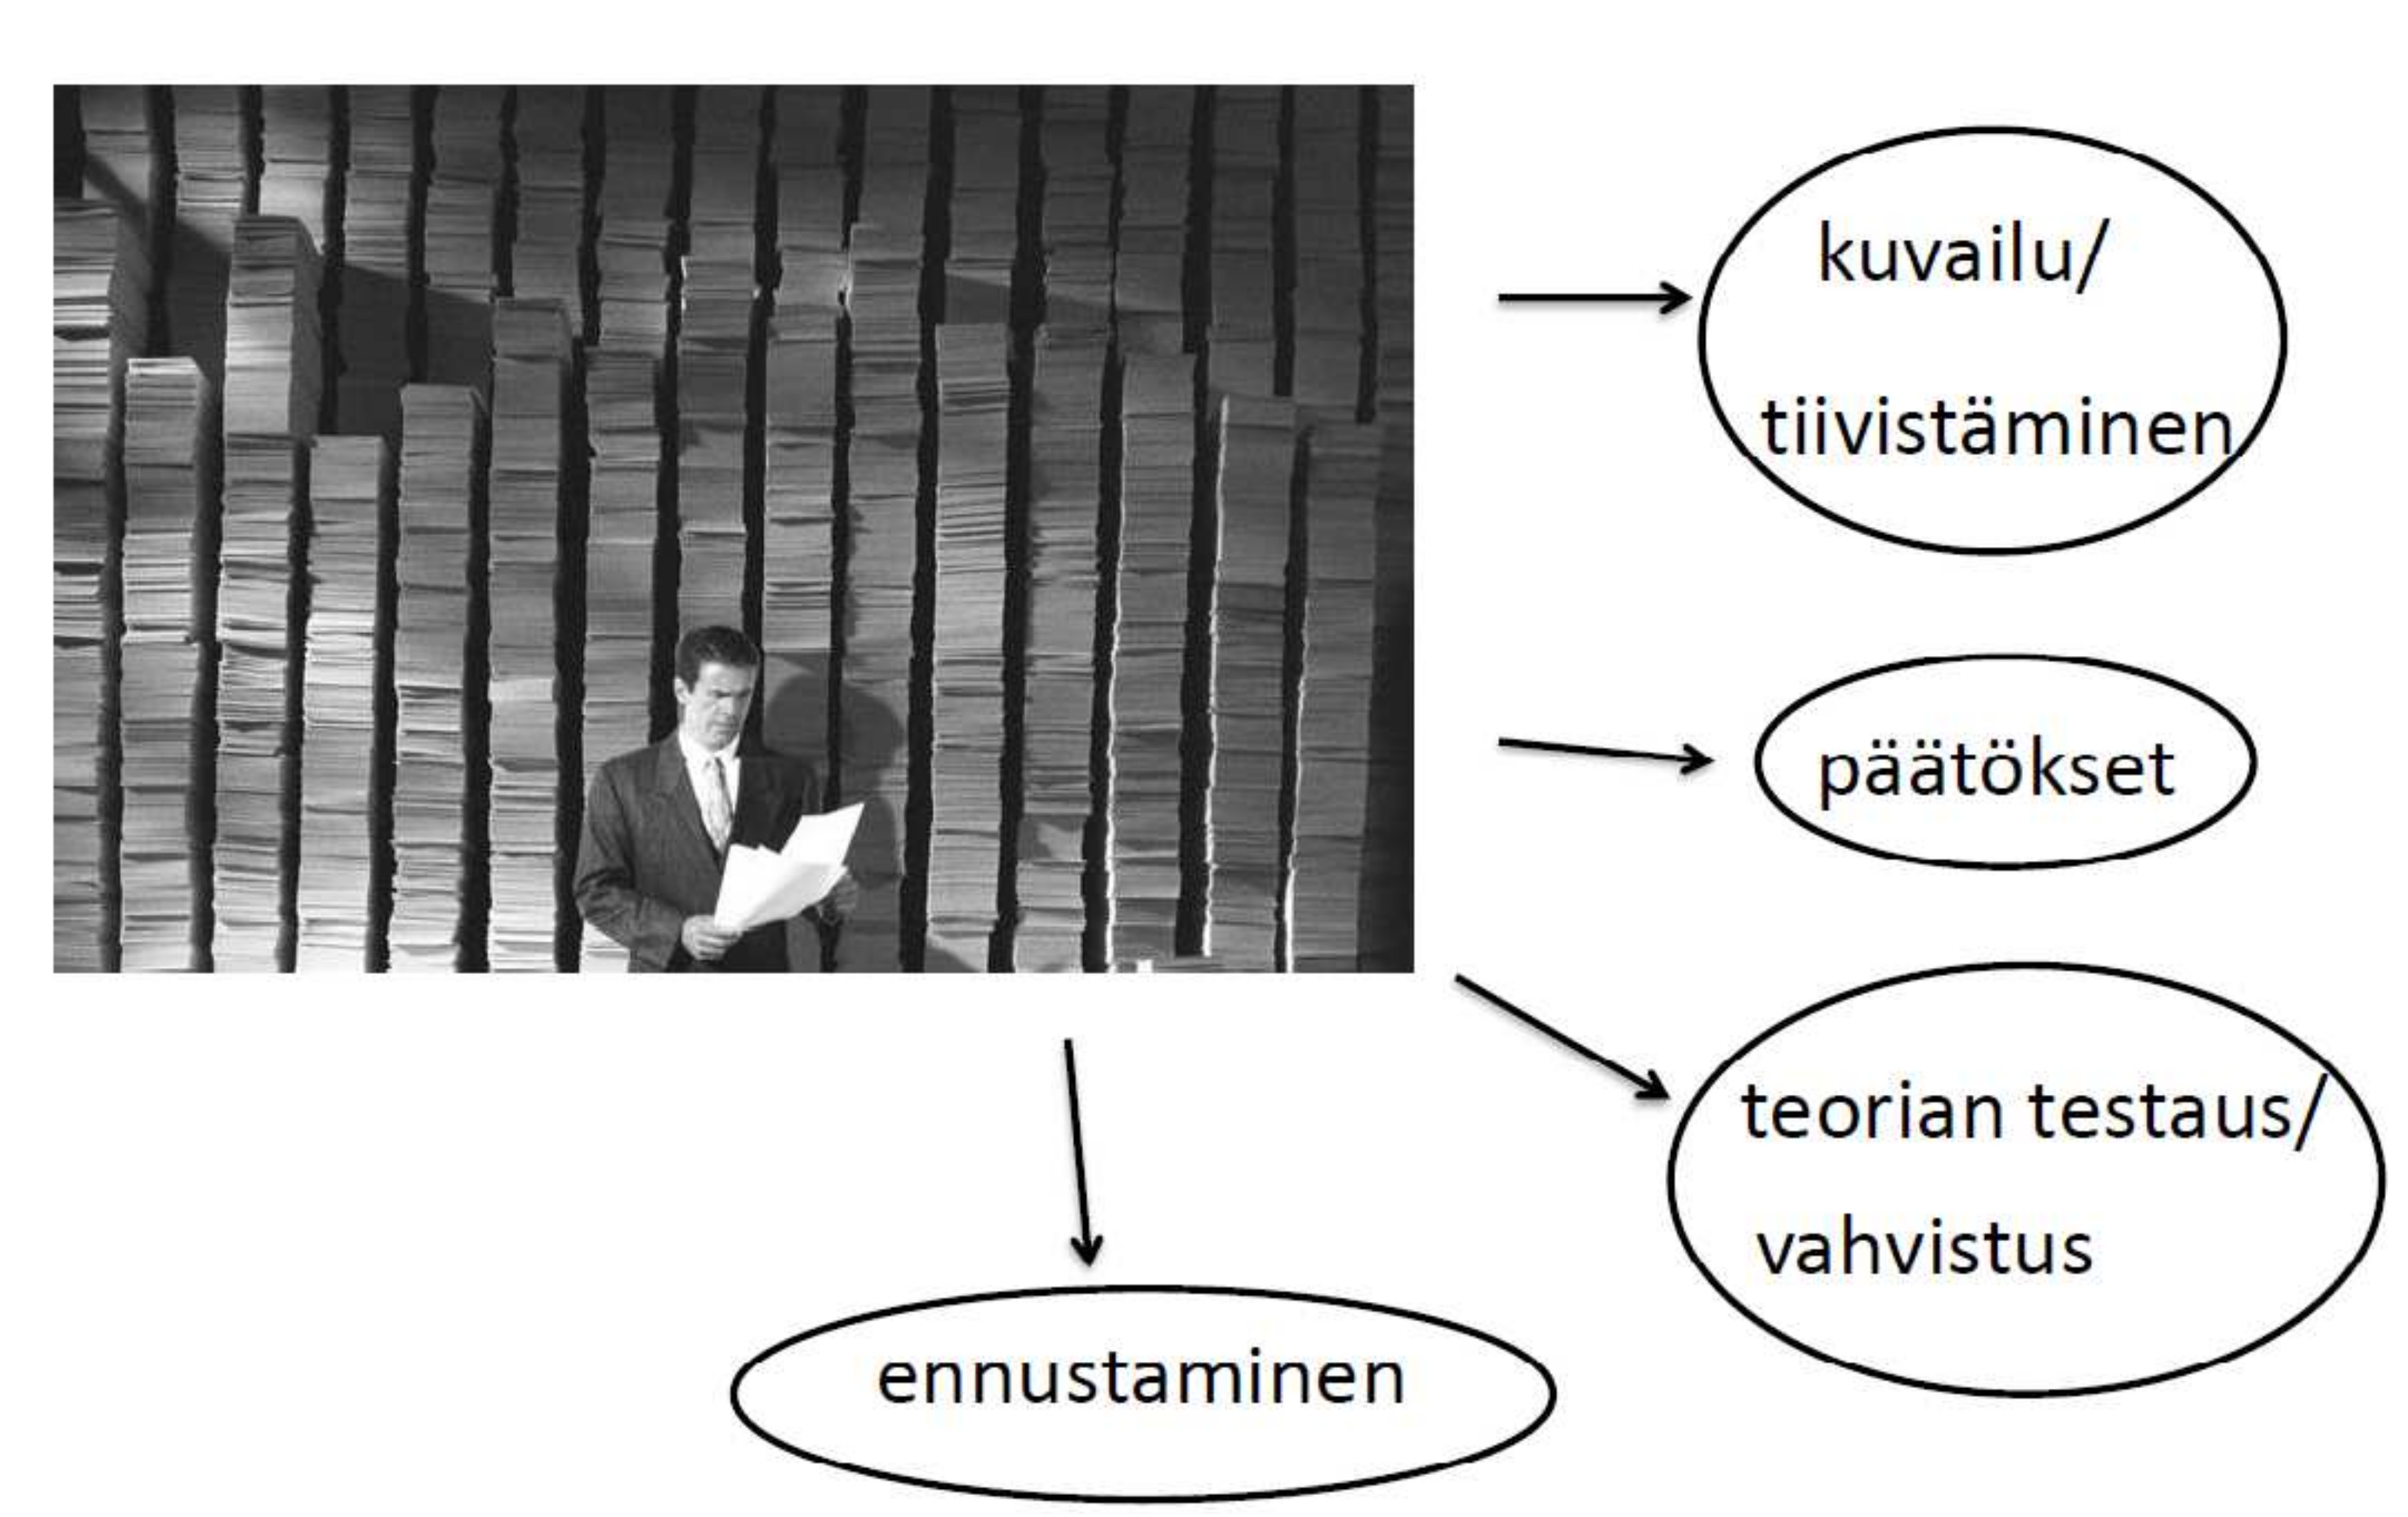
\includegraphics[width=1\linewidth]{images/soveltava} 

}

\caption{Soveltava tilastotiede}\label{fig:soveltava}
\end{figure}

\newpage

\textbf{Teoreettinen tilastotiede}

\begin{defblock}{}
\textbf{Teoreettinen tilastotiede}\\
kehittää (tilasto)matemaattisia malleja kuvaamaan satunnaisilmiöitä- ja prosesseja, jotka generoivat reaalimaailman ilmiöitä kuvaavia numeerisia tai kvantitatiivisia tietoja, joihin liittyy epävarmuutta ja satunnaisuutta.

\end{defblock}

\begin{itemize}
\tightlist
\item
  Teoreettinen tilastotiede luo pohjan tilastollisten menetelmien ymmärtämiselle, soveltamiselle ja kehittämiselle.

  \begin{itemize}
  \tightlist
  \item
    Ilman riittävää ymmärrystä tilastollisten menetelmien toimintaperiaatteista niiden soveltaja on vaarassa tehdä virhepäätelmiä! (ks. alaluku \ref{alaluku35} tilastotieteen kritiikistä)
  \end{itemize}
\item
  Mallit perustuvat todennäköisyyslaskentaan, ja niitä kutsutaan tilastollisiksi malleiksi, stokastisiksi malleiksi tai todennäköisyysmalleiksi.

  \begin{itemize}
  \tightlist
  \item
    Tilastolliset mallit perustuvat laajalti niin kutsuttuun uskottavuusfunktioon. Se on malli, joka riippuu havaintoaineiston lisäksi yhdestä tai useammasta parametrista. (ks. tarkemmin luku \ref{luku6})
  \item
    Uskottavuusfunktion arvo kertoo kuinka todennäköisenä voidaan havaittua aineistoa pitää, mikäli sen oletetaan olevan peräisin vastaavasta mallista jollain parametriarvoilla.
  \item
    Uskottavuuspäättelyn perusajatuksena on, että se tai ne parametriarvot, joilla uskottavuusfunktion arvo maksimoituu kuvaa aineiston generoinutta prosessia parhaiten.
  \item
    Aineistoa koskevia hypoteeseja voidaan testata käyttäen uskottavuusfunktion maksimia vastaavaa tilastollista mallia!
  \item
    \emph{``Kaikki mallit ovat vääriä, mutta jotkut ovat käyttökelpoisia.''} (Box, 1976).
  \end{itemize}
\end{itemize}

\hfill\break
\hfill\break

\begin{itemize}
\tightlist
\item
  Uskottavuusfunktiot perustuvat aina satunnaisilmiöiden mahdollisia arvoja kuvaaviin nk. \textbf{tiheysfunktioihin} tai \textbf{pistetodennäköisyysfunktioihin}.

  \begin{itemize}
  \tightlist
  \item
    Nämä funktiot kuvaavat jonkin satunnaismuuttujan (satunnaisilmiön) saamien arvojen jakaumaa.
  \item
    Esimerkiksi kolikonheitto on satunnaisilmiö ja sillä on vain kaksi arvoa\footnote{Kolikon kantilleen jäämistä ei tässä lasketa mahdolliseksi tapahtumaksi.} ja kolikonheittoa voidaan kuvata nk. binomijakaumalla, jota merkitään \(\text{Bin}(n,p)\), jossa \(n\) on heittojen lukumäärä ja \(p\) on kruunan todennäköisyys.
  \end{itemize}
\end{itemize}

\begin{eblock}{}

\textbf{Esimerkki: kolikonheitto}:

\begin{itemize}
\tightlist
\item
  Eräs klassinen yksinkertainen todennäköisyyslaskennassa ja tilastotieteessä käytettävä esimerkki käsittelee kolikonheittoa.
\item
  Kuvitellaan että olemme heittäneet kolikkoa 40 kertaa ja saatu kruuna 40/40 tapauksessa.

  \begin{itemize}
  \tightlist
  \item
    Kolikonheittoa seuranneet havainnot muodostavat nyt havaintoaineiston, jonka pohjalta voidaan perustellusti kysyä, että onko uskottavaa että kolikonheitto noudataa binomijakaumaa \(\text{Bin}(40, 0.5)\)?
  \item
    Toisin sanoen, kuinka uskottavana voidaan pitää sitä että kyseinen kolikkon on tavallinen, painottamaton kolikko?
  \end{itemize}
\end{itemize}

\end{eblock}

\begin{figure}

{\centering 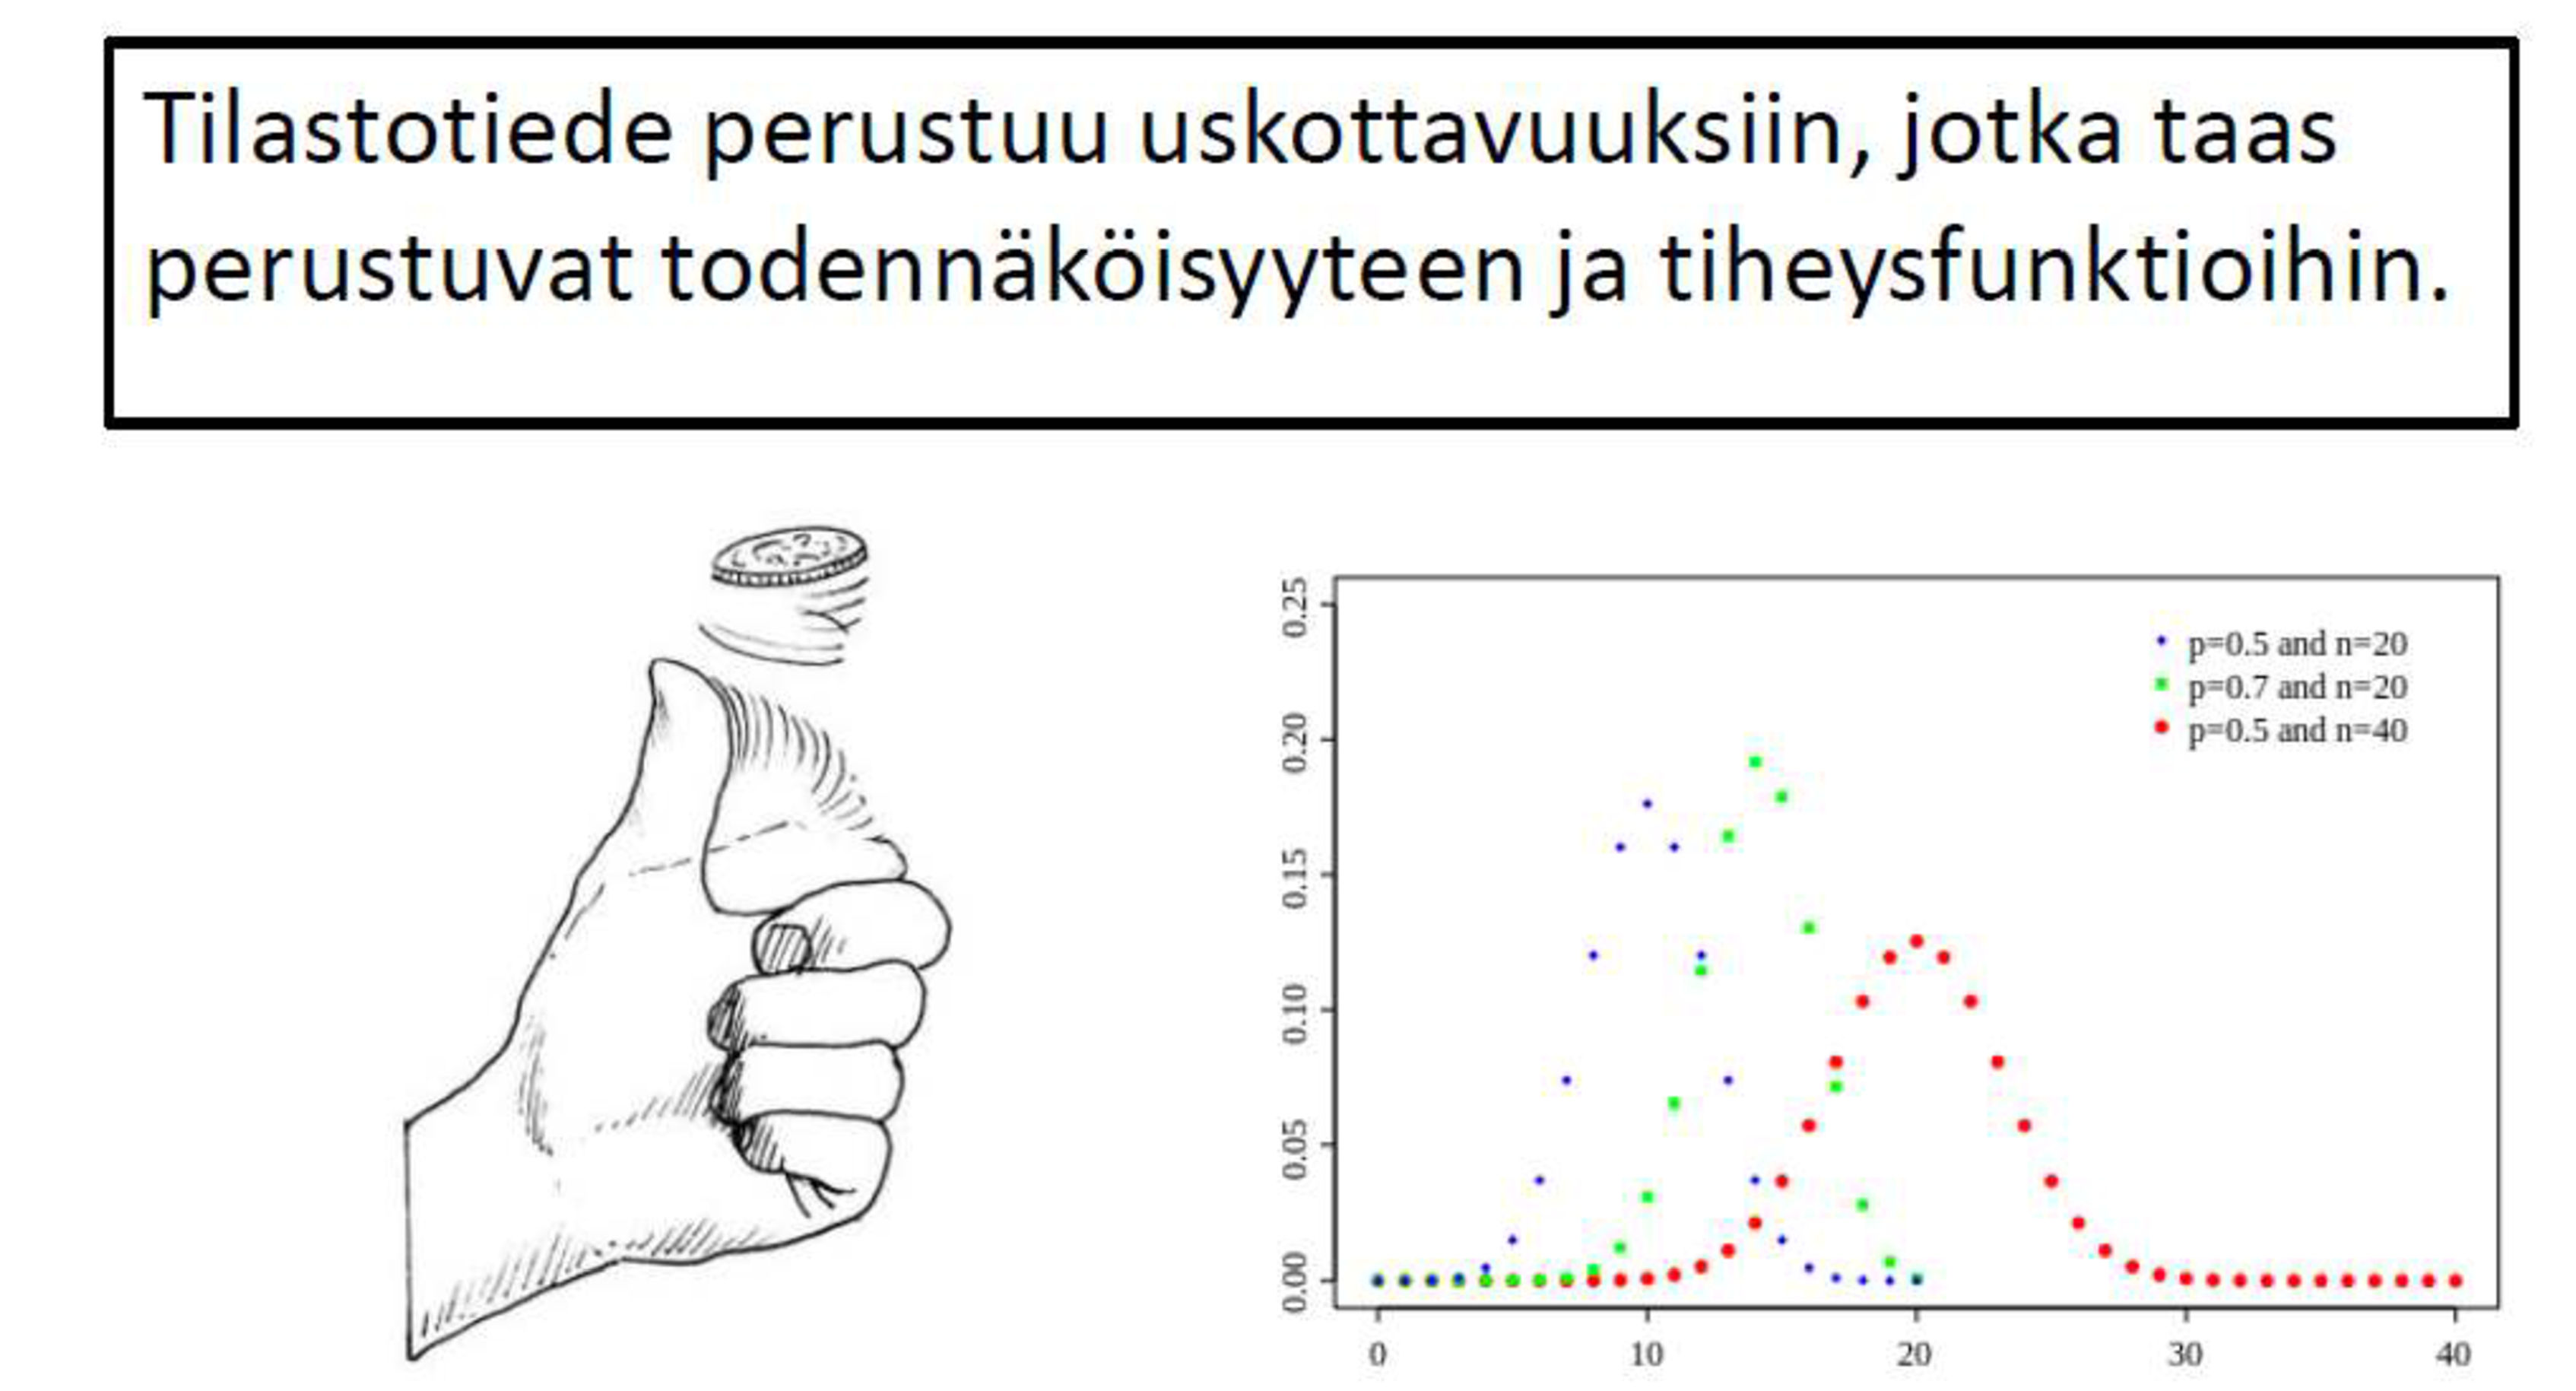
\includegraphics[width=1\linewidth]{images/perustuu} 

}

\caption{Tilastotiede ja todennäköisyys}\label{fig:perus}
\end{figure}

\hfill\break
\hfill\break

\begin{itemize}
\tightlist
\item
  \textbf{Todennäköisyyslaskenta} luo tilastotieteelliselle epävarmuuden mallintamiselle vahvan ja uskottavan matemaattisen perustan.

  \begin{itemize}
  \tightlist
  \item
    Todennäköisyyslaskentaa opetetaan tarkemmin (tätä kurssia seuraavilla) kursseilla \href{https://opas.peppi.utu.fi/fi/opintojakso/TILM3553/1734}{TILM3553 Todennäköisyyslaskennan peruskurssi pääaineopiskelijoille}, \href{https://opas.peppi.utu.fi/fi/opintojakso/TILM3568/3385}{TILM3568 Todennäköisyyslaskenta sivuaineopiskelijoille} ja \href{https://opas.peppi.utu.fi/fi/opintojakso/SMAT5306/4400}{SMAT5306 Todennäköisyyslaskennan jatkokurssi}.
  \end{itemize}
\end{itemize}

\begin{figure}

{\centering 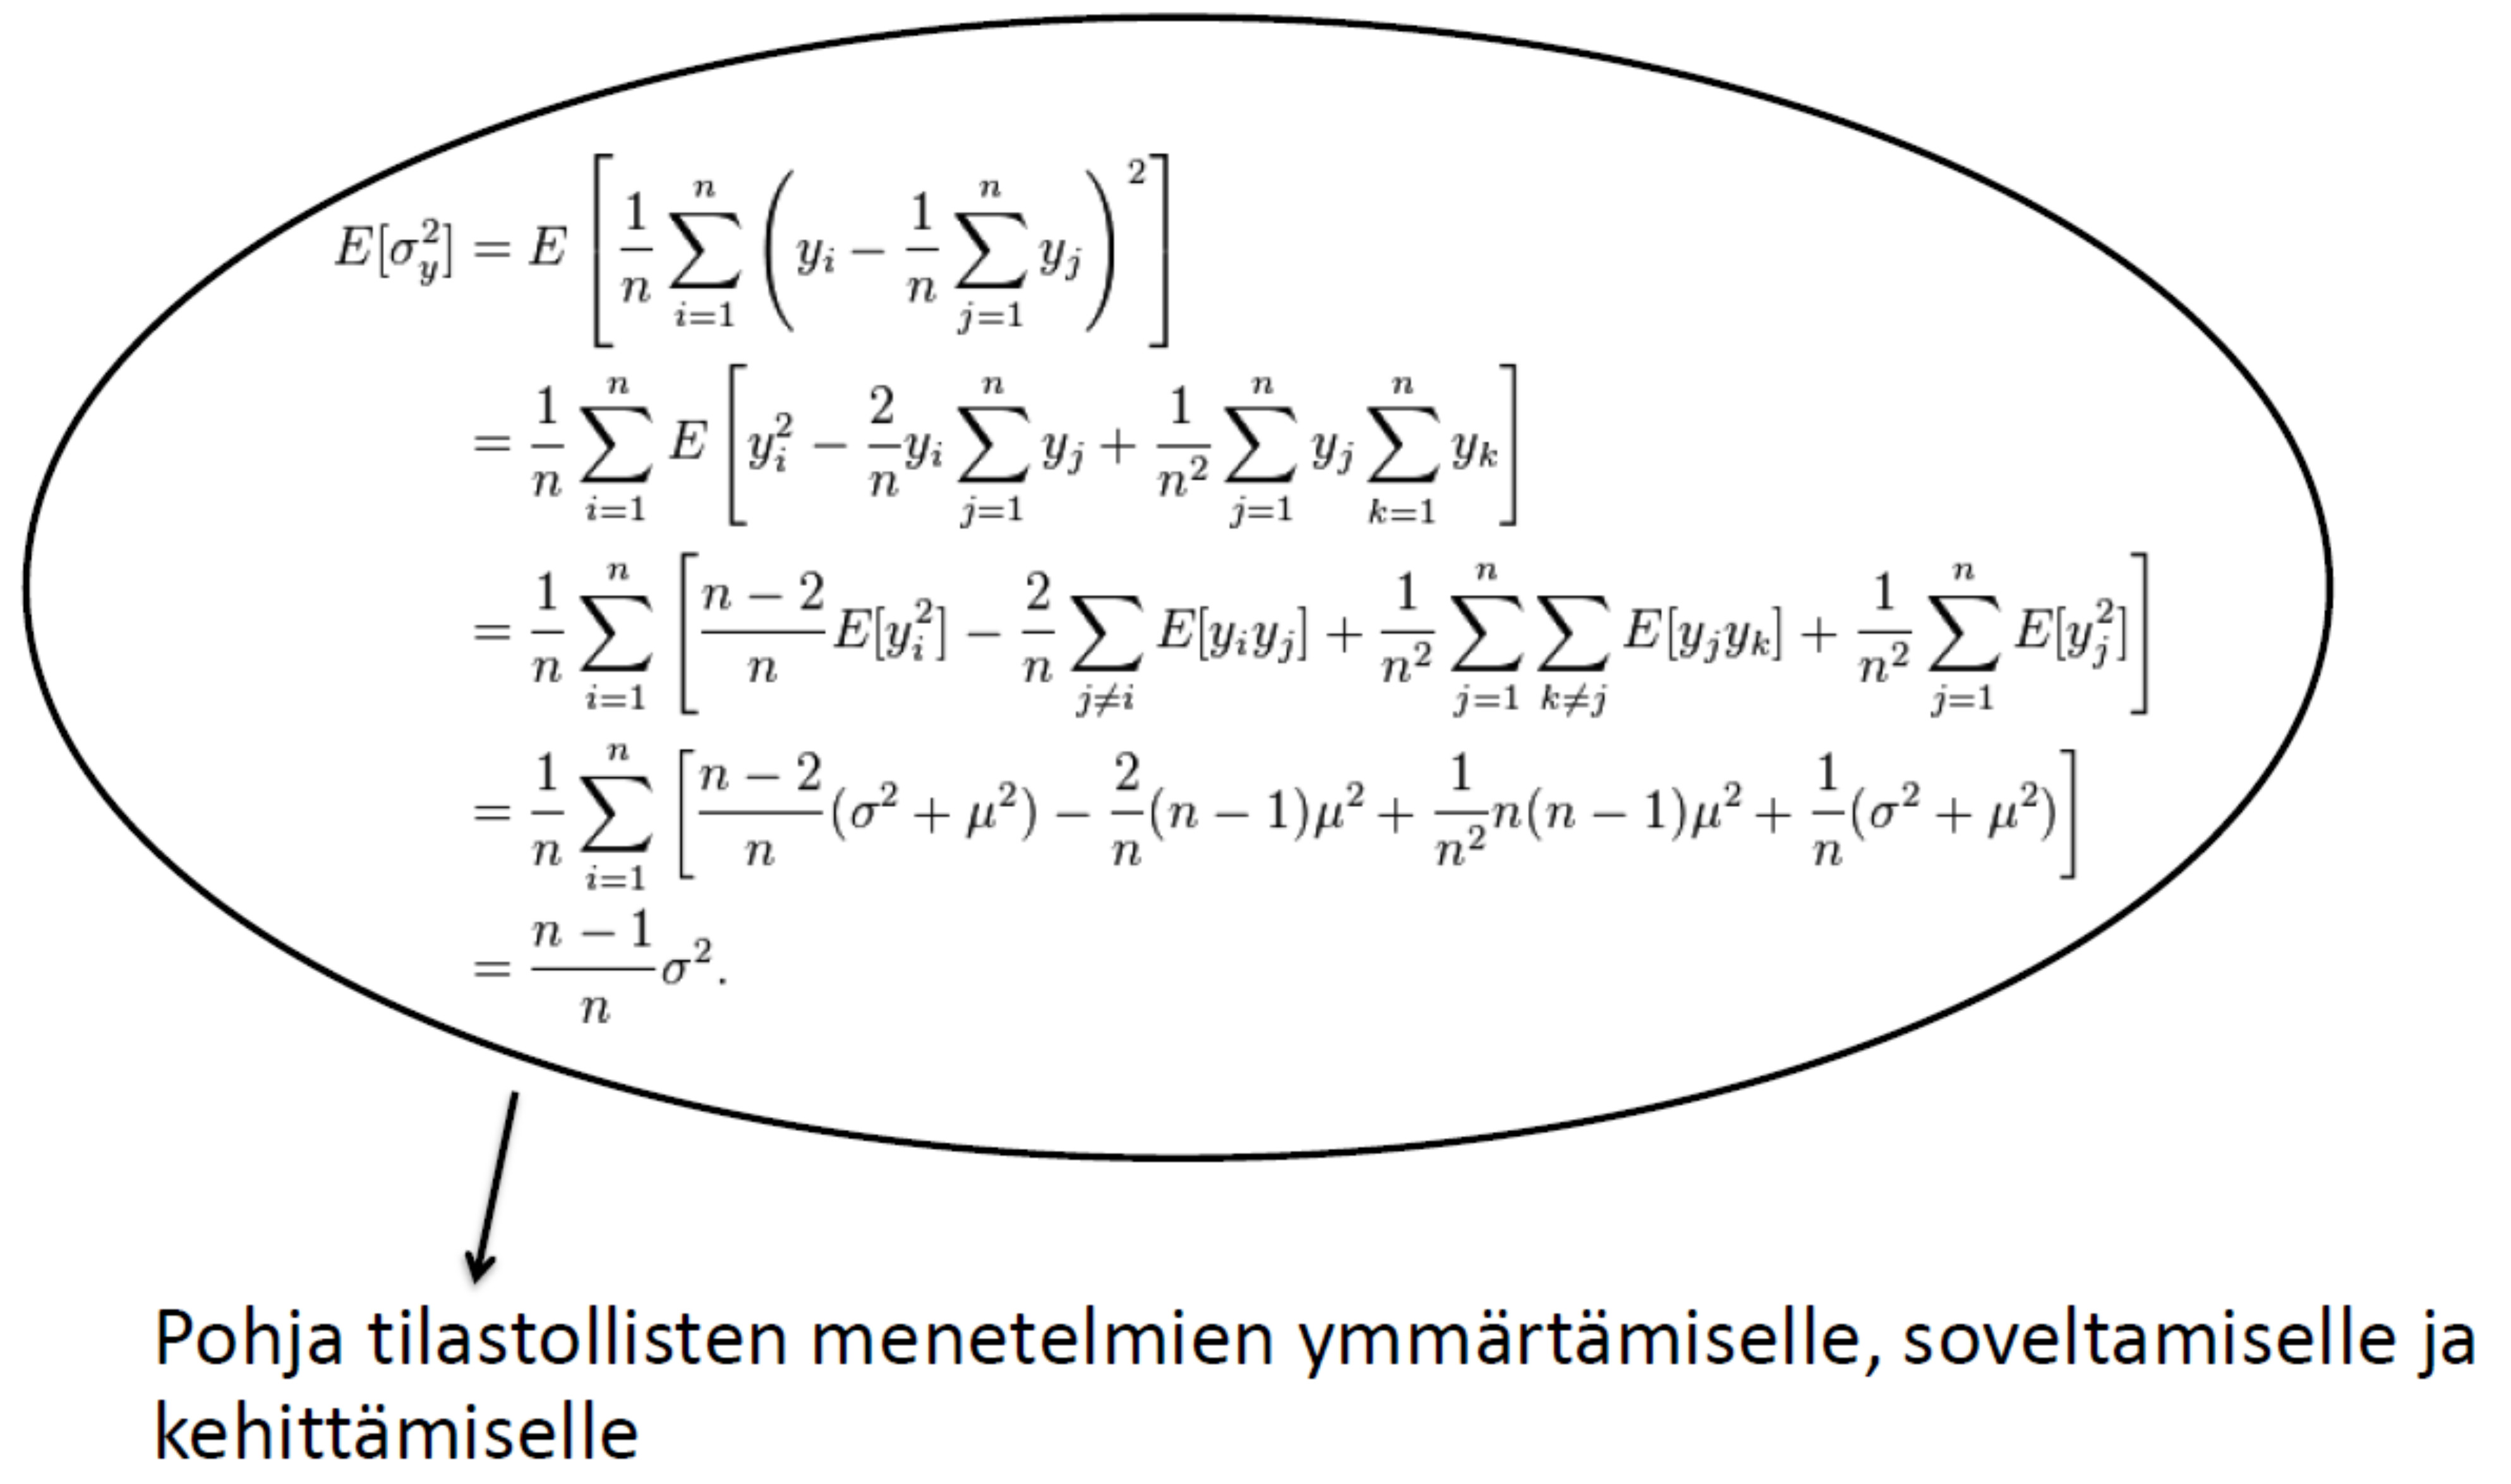
\includegraphics[width=1\linewidth]{images/teoreettinen} 

}

\caption{Esimerkki teoreettisesta tilastotieteestä ja tilastollisesta päättelystä.}\label{fig:teoreettinen}
\end{figure}

\newpage

\hypertarget{alaluku35}{%
\section{Tilastotieteen kritiikkiä}\label{alaluku35}}

\begin{itemize}
\tightlist
\item
  Tilastotieteen rooli tiedeyhteisössä on niin tärkeä että sitä kohtaan on ymmärrettävästi esitetty myös paljon kritiikkiä. Valtaosa kritiikistä kohdistuu joko tilastotieteen matemaattisuuteen tai sitten siinä tarvittaviin oletuksiin, jotka mahdollistavat esimerkiksi hypoteesien testaamisen.

  \begin{itemize}
  \tightlist
  \item
    Usein kritiikki on aiheetonta ja johtuu sen esittäjän puutteellisesta tilastotieteen ymmärryksestä. Perusteettoman kritiikin esittäminen toista tieteenalaa kohtaa ei kuitenkaan ole vieras ilmiö juuri millään alalla.
  \end{itemize}
\item
  Tässä alaluvussa käymme läpi yleisimpiä kritiikin muotoja, joita tilastotiedettä kohtaan esitetään ja pyrimme tarjoamaan vastauksia/vastineita silloin kun niitä voidaan antaa.
\end{itemize}

\hfill\break
\hfill\break

\textbf{``Yleismaailmallinen'' kritiikki}

\begin{itemize}
\tightlist
\item
  Aloitetaan yleismaailmallisella kritiikillä, jota tilastollista tutkimusta vastaan on esitetty:

  \begin{itemize}
  \tightlist
  \item
    Tilastotieteessä käytettävien tunnuslukujen, kuten keskiarvon, reaalimaailman vastineet ovat joskus mielivaltaisia. Esimerkiksi keskiarvo on ajoittain ongelmallinen tunnusluku, sillä lienee varsin selvää, että keskimääräistä ihmistä ei ole olemassa vaikka tilastotieteessä näitä tunnuslukuja usein lasketaankin.

    \begin{itemize}
    \tightlist
    \item
      Esimerkiksi puhekielessä yleinen nk. ``Keskiarvo-Kalle'', eli 1,8 lapsen vanhempi ja 1,5 auton omistaja on tietenkin täysin kuvitteellinen.
    \item
      Lisäksi joskus kuulee tilastotieteilijöitä kritisoitavan lausumalla ``\emph{Jos toinen jalka on jääkylmässä vedessä ja toinen kiehuvassa vedessä, niin tilastotieteilijän mielestä ihmisellä on tällöin keskimäärin hyvä olla}''
    \end{itemize}
  \end{itemize}
\item
  \textbf{Korrelaatio} on \textbf{tunnusluku}, joka kuvaa kahden muuttujan välistä riippuvuutta (palaamme tähän tarkemmin luvussa \ref{luku7}). Se ei kuitenkaan kuvaa millään tavoin \textbf{kausaalisuutta}, eli sitä kumpi aiheuttaa kumman, jos kumpikaan.\footnote{Tyler Vigen on kerännyt \href{https://www.tylervigen.com/spurious-correlations}{verkkosivuilleen (ks. linkki)} mitä moninaisimpia esimerkkejä kahdenvälisistä nk. \emph{näennäisistä} korrelaatioista.}

  \begin{itemize}
  \tightlist
  \item
    Esimerkiksi ``jäätelön syönti ja hukkumiskuolemat'' -tapauksessa havainnollisesti todetaan jäätelönkulutuksen ja hukkumiskuolemien lukumäärän korreloivan keskenään, mutta taustalla vaikuttava tekijä onkin lämmin kesä, joka vaikuttaa molempiin.
  \end{itemize}
\item
  Vaikkei näiden esimerkkien oikeellisuutta ole syytä kiistää, niin tilastollisen tiedon arvioinnissa on kuitenkin syytä päästä syvemmälle.
\end{itemize}

\hfill\break
\hfill\break

\textbf{Kritiikki matemaattisuutta kohtaan}

\begin{itemize}
\tightlist
\item
  Ehkä merkittävin kritiikki tilastollisia menetelmiä kohtaan kohdistuu kritiikin näkökulmasta perusteettomaan, tai ainakin liian vahvaan, matemaattisuuden tuomaan itsevarmuuteen. Voidaankin siis perustellusti kysyä, että \textbf{onko tieteellisyys = matemaattisuus}?

  \begin{itemize}
  \tightlist
  \item
    Useat tieteenalat käyttävät tutkimuksessaan edistyneitäkin tilastollisia menetelmiä siitä huolimatta, että tutkijoiden tilastomatemaattinen pohjakoulutus ei välttämättä ole riittävällä tasolla kyseisten menetelmien kokonaisvaltaiseen ymmärtämiseen.

    \begin{itemize}
    \tightlist
    \item
      Helppokäyttöisistä tilasto-ohjelmistoista on riittävät perustaidot omaaville käyttäjille erittäin paljon hyötyä mutta koneiden ja ohjelmien käytön opettelu ei kuitenkaan ole varsinaista tilastotiedettä (tarvitaan enemmän tilastotieteen opintoja).
    \item
      Laskentatehon ja modernin tietojenkäsittelyteknologian ansiosta monimutkaisiakin tilastollisia analyysejä on kuitenkin mahdollista tehdä vaikka tutkijalla olisi tilastotieteestä vain perustiedot, jos sitäkään.
    \item
      Pahimmillaan tämä saattaa johtaa siihen, että analyyseja tehdään ymmärtämättä mitä itse asiassa ollaan tekemässä.
    \end{itemize}
  \item
    Tilastollisten analyysien hyödyllisyyden ja järkevyyden ehtona on kuitenkin käytettävien menetelmien, aineiston ja tutkittavan ilmiön pintaa syvemmälle ulottuva tuntemus.

    \begin{itemize}
    \tightlist
    \item
      Käytettävien tilastollisten menetelmien oletukset on osattava ottaa huomioon ja toisaalta odottamattomien tulosten syyt on pystyttävä jäljittämään.

      \begin{itemize}
      \tightlist
      \item
        Teknistä esitystä käyttävää tutkijaa saatetaan pitää erityisen uskottavana, koska hän kykenee käyttämään vaikeita menetelmiä. Tästä huolimatta tutkimusongelma ei saisi päästä unohtumaan.
      \item
        Tutkijan tulisikin varmistua siitä, että käytettävät menetelmät todella vastaavat asetettuihin tutkimuskysymyksiin ja että tutkimusongelma on ratkaistavissa käytettävillä menetelmillä.
      \item
        Tekninen esitys ei takaa onnistunutta tilastollista tutkimusta eri näkökulmista katsoen. Monet tilastolliset menetelmät ovat vaikeita ja vaativat soveltajiltaan paljon.
      \item
        Lisäksi on hyvä muistaa, että käytettävien menetelmien lähtökohdat ja oletukset eivät matemaattisuudestaan huolimatta ole välttämättä neutraaleja!
      \end{itemize}
    \item
      Kaikkia tieteentekijöitä ei voida velvoittaa opiskelemaan edistynyttä abstraktia tilastotieteen teoriaa (tilastomatematiikkaa), mutta menetelmien oikeaoppinen käyttö kuitenkin vaatii riittävää ymmärrystä.
    \end{itemize}
  \end{itemize}
\end{itemize}

\hfill\break
\hfill\break

\textbf{Kritiikki yksinkertaistuksia kohtaan}

\begin{itemize}
\tightlist
\item
  Edellisiä kohtia yleisemmin tilastotiedettä on kritisoitu siitä, että se ei kykene riittävällä tasolla huomioimaan reaalimaailman kompleksisuutta.

  \begin{itemize}
  \tightlist
  \item
    Merkittävässä osassa tilastollisia analyyseja lähtökohtana on usko ``todellisen'' maailman ja näin ollen aineistoa generoivien mekanismien olemassaoloon.

    \begin{itemize}
    \tightlist
    \item
      Tätä saatetaan usein pitää kuitenkin kyseenalaisena: voiko ``tosielämän stokastiikasta'' muka todella löytyä säännönmukaisuuksia?
    \item
      Tämä kysymys on kuitenkin pitkälti tieteenfilosofinen ja palautuu lopulta sovellusalaan sekä tutkimusongelmaan ja -kysymykseen: tilastollisten menetelmien toimivuutta voidaan helposti testata esimerkiksi simulaatiokokeilla.\\
    \end{itemize}
  \item
    Tilastotiedettä on myös kritisoitu sen ``sokeudesta'' sosiaaliseen vuorovaikutukseen liittyviin subjektiivisiin kokemuksiin kuten tunteisiin, kokemuksiin ja ei-numeeriisiin havaintoihin.

    \begin{itemize}
    \tightlist
    \item
      Tämä kritiikki ei kuitenkaan suoranaisesti ole tilastotieteen kritiikkiä, vaan jälleen sovellusalakohtainen ja erityisesti tutkimuskysymyksen asettelua koskeva ongelma.

      \begin{itemize}
      \tightlist
      \item
        Tuntemuksia ja kokemuksia voidaan hyvin testata tilastollisin menetelmin, mikäli tutkija osaa uskottavasti määritellä niille numeerisen mittauksen kriteeristöt!
      \item
        Tämä on kuitenkin vaikeaa, sillä aivan kaikkea ei voida kvantifioida: kirjoitetun tekstin tai sosiaalisten merkitysten tulkinnan sekä elämysten kuten musiikin ja taiteen aiheuttamien mielikuvien ja tunteiden voidaan perustellusti nähdä olevan hyvin haastavia kvantifioida.
      \end{itemize}
    \item
      Näiden aiheiden tulkinta, ymmärtäminen ja tutkiminen ulottuu kvantitatiivisen tutkimuksen ulkopuolelle.
    \end{itemize}
  \item
    Mikäli tutkittavasta ilmiöstä pystyy kvantitatiivisilla mittauksilla saada relevanttia tietoa, tulisi aineiston analyysin apuna joka tapauksessa aina käyttää tilastollisia menetelmiä!
  \item
    Vaikka kvantitatiivisia aineistoja ei voi pitää objektiivisina faktoina asioiden tilasta, se ei tarkoita, etteivätkö tulokset voisi olla käyttökelpoisia.
  \end{itemize}
\end{itemize}

\hfill\break
\hfill\break

\textbf{Temppukokoelmakritiikki}

\begin{itemize}
\tightlist
\item
  Eräs ehkä osin implisiittinen kritiikki tilastotiedettä kohtaan on sen pitäminen nk. \textbf{``temppukokoelmana''.}

  \begin{itemize}
  \tightlist
  \item
    Tilastotieteen voi nähdä koostuvan numeeristen tietojen jalostamisen menetelmistä. Tämä näkemys, joka on usein tahaton, pelkistää tilastotieteen \emph{vain} \textbf{menetelmäkokoelmaksi}, vailla omaa teoriaa.
  \item
    Eri tutkimusalojen empiirisessä työssä (liian) usein vain kerätään aineisto ja vasta sitten mietitään mitä sillä voitaisiin tehdä.
  \item
    Usein apuun haetaan tilastotieteilijä, jonka odotetaan loihtivan (tilastollisen) ratkaisun ongelmaan kuin ongelmaan.

    \begin{itemize}
    \tightlist
    \item
      Joskus tämä toki onnistuukin, mutta useimmiten ei.
    \item
      Tilastotiede ei siis ole ``työkalupakki'', josta valitsemalla oikeanlaisen menetelmän voi vastata mihin tahansa tutkimuskysymykseen!
    \end{itemize}
  \item
    Tilastolliset menetelmät tulee ymmärtää ja niitä tulee soveltaa kaikissa soveltavan tutkimuksen vaiheissa, jotta tutkimusongelmaan kyetään vastaamaan eikä turhaa työtä tule tehdyksi.
  \item
    Karkeasti luokitellen tilastotieteilijät kehittävät menetelmiä, joita soveltajat käyttävät.

    \begin{itemize}
    \tightlist
    \item
      Soveltavia tilastotieteilijöitä löytyy kuitenkin yhä kiihtyvissä määrin! Erityisesti eri rajatieteiden alueilla, kuten alaluvussa \ref{alaluku36} lyhyesti esitellään.
    \end{itemize}
  \end{itemize}
\end{itemize}

\textbf{Tilastotieteen väärinkäyttö}

\begin{itemize}
\tightlist
\item
  Tilastotiedettä on myös mahdollista käyttää väärin monin eri tavoin, joka edelleen altistaa koko tieteenalan (perusteettomalle) kritiikille!

  \begin{itemize}
  \tightlist
  \item
    Tilastoja ja tilastotiedettä käytetään paljon väärin, mutta tämä on usein tahatonta (esim. puutteellisesta koulutuksesta johtuvaa).

    \begin{itemize}
    \tightlist
    \item
      Joskus kuitenkin näkee tarkoituksellista tilastojen vääristelyä tai tahallista tilastollisten menetelmien väärinkäyttöä!
    \item
      Kansalaisten tiedelukutaidon ja tilastollisten menetelmien tuntemuksen merkitys on kasvanut viime vuosikymmeninä ja kasvanee jatkossa yhä, kun esimerkiksi erilaiset ``vaihtoehtotieteet'' ovat nousseet suositummiksi.
    \item
      Tilastotieteen ymmärrys auttaa itse kutakin tunnistamaan virheellisiä tai puutteellisin tiedoin tehtyjä päätelmiä ja täten helpottaa tietoyhteiskunnassa toimimista ja kriittistä ajattelua!
    \end{itemize}
  \end{itemize}
\item
  Yleisiä tilastollisten menetelmien väärinkäyttötapoja ovat esimerkiksi seuraavat:

  \begin{itemize}
  \tightlist
  \item
    \textbf{``Kolmannen tyypin virhe''}: kun tilastollisia menetelmiä käyttämällä saadaan oikeita vastauksia, mutta vääriin kysymyksiin! Esimerkiksi jos tutkija ei täysin ymmärrä minkälaisia vastauksia käytettävissä olevasta aineistosta ja valitulla menetelmällä voidaan saada, voi hän syyllistyä kolmannen tyypin virheeseen. Tällöin voi nimittäin käydä niin, että hän tulkitsee tilastolliset testit täysin oikein, mutta luulee väärin niiden vastaavaan eri kysymykseen kuin on esitetty.
  \item
    Black-box ilmiö: saadaan \emph{ehkä} oikeita vastauksia, mutta ei tiedetä \emph{miksi} ja \emph{mihin} kysymyksiin.

    \begin{itemize}
    \tightlist
    \item
      Totaalinen tilastollisen päättelyn osaamattomuus saattaa johtaa tutkijan täysin väärille urille ja esimerkiksi jokseenkin epäoleelliseen tekniseen näpertelyyn monimutkaisten mallien kanssa.
    \end{itemize}
  \end{itemize}
\end{itemize}

\begin{eblock}{}

\textbf{Esimerkki: Kolmannen tyypin virhe}

\begin{itemize}
\tightlist
\item
  Oletetaan että haluat tutkia onko kahden eri ikäryhmän ihmisten pituuksissa eroja ja sinulla on käytettävissä edustava otos molempien ikäluokkien edustajista.
\item
  Päätät tutkia \emph{yksisuuntaisesti} onko toisen ryhmän, ryhmän A, keskipituus \emph{pienempi} kuin ryhmän B.

  \begin{itemize}
  \tightlist
  \item
    Testitulos osoittaa, että voit hylätä nollahypoteesin, jonka mukaan ryhmien \emph{keskipituus olisi sama}.
  \item
    Kolmannen tyypin virhe syntyy silloin, jos tosiasiallisesti testin hylkääminen johtui siitä, että ryhmän A keskipituus olikin \emph{suurempi} kuin ryhmän B keskipituus, mutta tätä et testin tuloksen perusteella voi tietää!\\
  \end{itemize}
\end{itemize}

\end{eblock}

\hypertarget{alaluku36}{%
\section{Tilastotieteen sovellusaloja ja ``rajatieteitä''}\label{alaluku36}}

\begin{itemize}
\item
  Yleisenä menetelmätieteenä tilastotiedettä sovelletaan useilla eri tieteenaloilla.

  \begin{itemize}
  \tightlist
  \item
    Jokaisella sovellusalalla on oma erillinen teoriapohjansa sekä empiiriset käytänteet, joten substanssitietous on sovellettaessa erityisen tärkeää.

    \begin{itemize}
    \tightlist
    \item
      Huolimatta vaihtelevista empiirisistä käytännöistä sovellusmenetelmän taustalla on (lähes aina) kuitenkin tilastotieteen alalla kehitetty menetelmä.
    \item
      Sovellusaloilla ongelmanratkaisussa yhdistetäänkin metodiseen osaamiseen välttämättä myös substanssitietoutta. Tämän myötä soveltavan tilastollisen tutkimuksen kenttä on laaja ja rikas.
    \end{itemize}
  \item
    Osa näistä sovelluskentistä on kehittynyt vahvassa yhteisvaikutuksessa tilastotieteen ja lähitieteiden (viime aikoina erityisesti koneoppimisen) yhteydessä.
  \end{itemize}
\item
  Usein on pystyttävä arvioimaan ongelmanasettelun ja tulosten tarkoituksenmukaisuutta ja pyrkiä välttymään siltä että tutkijan tieteelliset ja yhteisölliset sitoumukset heijastuisivat tutkimuksen kulkuun.
\item
  Tilastotieteen pääaineopiskelun osalta substanssitietous saavutetaan usein sivuaineopintojen perusteella. Vastaavasti toisinpäin muiden aineiden pääaineopiskelijoiden kohdalla, jolloin tilastotiede voi yhtä hyvin toimia (laajalti opiskeltuna) vahvana sivuaineena.
\item
  Jokaisella tieteenalalla, jonka tutkimusaineistot voidaan esittää numeerisessa tai kvantitatiivisessa muodossa voi soveltaa/voisi soveltaa/pitäisi soveltaa tilastollisia menetelmiä sekä tutkimusaineistoja kerättäessä että niitä analysoitaessa.

  \begin{itemize}
  \tightlist
  \item
    Siten jokainen empiirisen tutkimuksen havaintoaineisto on tilastollisen tutkimuksen mahdollinen kohde.
  \item
    Esim. kokeellinen tutkimus käyttää apunaan tilastollisia menetelmiä.
  \end{itemize}
\item
  Koska tilastotieteellä on sovelluksensa miltei kaikilta tieteenhaaroilla, on syntynyt nk. ``rajatieteitä'':

  \begin{itemize}
  \tightlist
  \item
    Sovellusaloja, joilla tilastotieteen soveltaminen on muodostunut omaksi tutkimuskohteekseen/tieteenlajikseen (ks. linkit):

    \begin{itemize}
    \tightlist
    \item
      \href{https://en.wikipedia.org/wiki/Psychometrics}{Psykologia: psykometriikka,}
    \item
      \href{https://en.wikipedia.org/wiki/Sociometry}{Sosiaalitieteet: sosiometria,}
    \item
      \href{https://en.wikipedia.org/wiki/Econometrics}{Taloustiede: ekonometria,}
    \item
      \href{https://en.wikipedia.org/wiki/Chemometrics}{Kemia: kemometria,}
    \item
      \href{https://en.wikipedia.org/wiki/Biometrics}{Bio- ja lääketiede: biometria,}
    \item
      \href{https://en.wikipedia.org/wiki/Epidemiology}{Epidemiologia,}
    \end{itemize}
  \item
    Soveltavan matematiikan tutkimusaloja, jotka ovat osaltaan päällekkäisiä tilastotieteen kanssa

    \begin{itemize}
    \tightlist
    \item
      \href{https://en.wikipedia.org/wiki/Information_theory}{Informaatioteoria,}
    \item
      \href{https://en.wikipedia.org/wiki/Mathematical_statistics}{Matemaattinen tilastotiede,}
    \item
      \href{https://en.wikipedia.org/wiki/Probability}{Todennäkäsyyslaskenta,}
    \item
      \href{https://en.wikipedia.org/wiki/Operations_research}{Operaatioanalyysi}
    \end{itemize}
  \item
    Tietojenkäsittelytieteen alaan (osittain) lukeutuvia tutkimusaloja

    \begin{itemize}
    \tightlist
    \item
      \href{https://en.wikipedia.org/wiki/Computational_science}{Laskennalliset menetelmät,}
    \item
      \href{https://en.wikipedia.org/wiki/Data_mining}{Data mining,}
    \item
      \href{https://en.wikipedia.org/wiki/Knowledge_extraction}{Knowledge discovery,}
    \item
      \href{https://en.wikipedia.org/wiki/Pattern_recognition}{Hahmontunnistus,}
    \item
      \href{https://en.wikipedia.org/wiki/Artificial_intelligence}{Tekoäly,}
    \item
      \href{https://en.wikipedia.org/wiki/Machine_learning}{Koneoppiminen}
    \end{itemize}
  \end{itemize}
\item
  Ja paljon muita!
\end{itemize}

\hypertarget{luvun-3-yhteenveto-keskeisiuxe4-termejuxe4-ja-kokonaisuuksia.}{%
\section{Luvun 3 yhteenveto, keskeisiä termejä ja kokonaisuuksia.}\label{luvun-3-yhteenveto-keskeisiuxe4-termejuxe4-ja-kokonaisuuksia.}}

Tilastotieteen perustermejä:
- Populaatio
- Tilastoyksikkö ja tilastollinen muuttuja
- Havainto
- Havaintoaineisto eli data

Mitä tilastotiede on ja mitä se ei ole?
- Tilastotieteen suhde lähitieteisiin, kuten matematiikkaan, tietojenkäsittelytieteeseen ja datatieteeseen.

Tilastotieteen osa-alueet
- Soveltava tilastotiede (ml. kvantitatiivinen ja kvalitatiivinen tutkimus)
- Teoreettinen tilastotiede (tilastollisen mallin ajatus ja merkitys)

Tilastotieteen sovellusalat ja ``rajatieteet'' (ks. tarkemmin luentomoniste ja sieltä löytyvät linkit!)

Tilastotieteen kritiikki

\hypertarget{luku4}{%
\chapter{Sattuma ja satunnaisuus tilastotieteessä}\label{luku4}}

\begin{figure}

{\centering 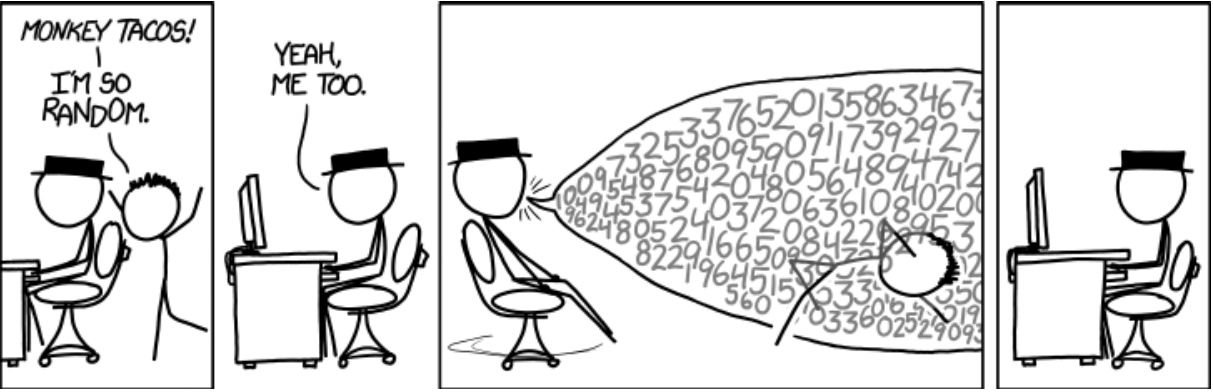
\includegraphics[width=1\linewidth]{images/im_so_random} 

}

\caption{Hauska kuva satunnaisuudesta.}\label{fig:random}
\end{figure}

Tässä luvussa pohdimme sattuman ja satunnaisuuden roolia tilastotieteessä ja tieteessä ylipäätään. Satunnaisuudella tarkoitetaan yleensä säännönmukaisuuden puuttumista ja ennustamattomuutta ja kenties juuri siksi sitä voidaan pitää yhtenä maailman vaikuttavimmista ilmiöistä. Jokainen haluaisi tietää mitä tuleman pitää ja siksi sattuma tekee elämästä mielenkiintoista: se vaikuttaa ja muokkaa niin meitä itseämme kuin ympäröivää maailmaa mitä merkityksellisimmin tavoin - joskus jopa vasten tahtoamme ja usein vailla täyttä ymmärtystämme!

Ihmisen oma kokemus on kuitenkin altis kaikenlaisille virhepäätelmille, joita kutsutaan myös kognitiivisiksi vinoumiksi. Haluamme löytää systematiikkaa ja tarkoitusta kaaoksesta sekä merkityksiä ja syy-seuraussuhteita sellaisista tapahtumista, jotka kuuluvat normaalivaihtelun piiriin. Tällaisissa tilanteissa usein tilastollinen tarkastelu paljastaakin ilmiön todellisen, alkuperäisestä kuvitelmasta poikkeavan luonteen. Erottaakseen systemaattinen vaihtelu satunnaisesta ja ymmärtääkseen oikeasti merkityksellisiä syy-seuraussuhteita, satunnaisuutta on välttämätöntä ymmärtää. Tämä välttämättömyys pätee erityisesti tiedeyhteisön jäseniin, jotka pyrkivät tutkimaan ympäröivän maailman satunnaisia ilmiöitä. Tilastotiede perustuu satunnaisilmiöiden ja satunnaisen aineiston tutkimiseen, joten sen ymmärtäminen on keskeisessä roolissa niin tilastotieteen kuin muidenkin tieteiden sekä lopulta maailman ymmärtämisessä.

\hypertarget{alaluku41}{%
\section{Satunnaisilmiöt ja satunnaismuuttujat tilastotieteessä}\label{alaluku41}}

\begin{itemize}
\tightlist
\item
  Edellisestä luvusta muistamme, että tilastotieteellisen tutkimuksen kohteena on aina jokin tilastoyksikköjen tutkimusmuuttujista koostuva havaintoaineisto, jonka pohjalta tehdään päätelmiä perusjoukosta/populaatiosta.
\item
  Nämä tilastolliset muuttujat tulkitaan satunnaisiksi, ja täten tilastollisen tutkimuksen tavoite on tutkia satunnaisilmiötä, joka on generoinut nämä havaitut eli toteutuneet arvot.

  \begin{itemize}
  \tightlist
  \item
    Yksi tilastotieteen olennainen tehtävä onkin kehittää \textbf{tilastollisia malleja}, joiden avulla satunnaisilmiöitä voidaan kuvata, selittää ja ennustaa.
  \item
    Tilastollisen mallin satunnaisten piirteiden kuvaus perustuu \textbf{todennäköisyyslaskentaan}.
  \end{itemize}
\end{itemize}

\begin{defblock}{}

\textbf{Satunnaisilmiö}

Reaalimaailman ilmiö on satunnaisilmiö, jos seuraavat ehdot pätevät:

\begin{itemize}
\tightlist
\item
  Ilmiöllä on useita erilaisia tulosvaihtoehtoja.
\item
  Sattuma määrää mikä tulosvaihtoehdoista toteutuu, eli yksittäistä tulosta ei voida tietää etukäteen.
\item
  Vaikka tulos vaihtelee ilmiön toistuessa satunnaisesti, käyttäytyy tulosvaihtoehtojen suhteellisten osuuksien jakauma tilastollisesti stabiilisti ilmiön toistokertojen lukumäärän kasvaessa.
\end{itemize}

\end{defblock}

\begin{itemize}
\tightlist
\item
  \textbf{Tilastollisella stabiiliudella} tarkoitetaan sitä, että on mahdollista arvioida kuinka \textbf{todennäköisiä} erilaiset tapahtumat, eli satunnaisilmiön tulosvaihtoehdot ovat.

  \begin{itemize}
  \tightlist
  \item
    Toisin sanoen satunnaisilmiön tulosvaihtoehtoihin on liityttävä säännönmukaisuutta, jonka on tultava esille ilmiön toistuessa.
  \end{itemize}
\end{itemize}

\begin{eblock}{}

\textbf{Esimerkkejä satunnaisilmiöistä}

\begin{itemize}
\tightlist
\item
  Helpoin esimerkki on uhkapelit, kuten kortti- ja noppapelit, arpajaiset, lotto tai ruletti: näitä käytetäänkin usein todennäköisyyslaskennan peruskursseilla satunnaisilmiöiden esittelyyn.
\item
  Lukion biologian tunneilta muistetaan, että perinnöllisyyskin on osaltaan sattumaa: se määrää kummalta vanhemmalta perittävä geenikopio on peräisin.

  \begin{itemize}
  \tightlist
  \item
    Vastaavasti populaatiotasolla eri ominaisuuksien jakautuminen yksilöiden ja populaatioiden välillä on satunnaista.
  \item
    Populaatiotaso voi tässä tarkoittaa esimerkiksi erilaisten eliöiden eri alueilla eläviä populaatioita, joiden välisiä eroja pyritään tutkimaan ja selittämään.
  \item
    Vastaavasti ihmisten, ihmisryhmien ja ihmisten muodostamien organisaatioiden sisäisessä ja välisessä käyttäytymisessä on useita satunnaisia elementtejä.
  \end{itemize}
\item
  Jopa deterministiseen toimintaperiaatteeseen tähtäävissä tehdastuotannossa käy satunnaisia virheitä tuotteiden valmistusprosesseissa, jotka ilmenevät esimerkiksi viallisina tuotteina.
\item
  Vastaavasti luonnontieteellisiin mittauksiin liittyy mittausvirheitä, jotka kuuluvat satunnaisvaihtelun piiriin. Esimerkiksi varhaisissa valonnopeusmittauksissa mittausvirheet saattoivat olla suuriakin!
\item
  Myös kvanttimekaniikan ja hiukkasfysiikan tutkimat ilmiöt ovat perusluonteeltaan satunnaisia.
\end{itemize}

\end{eblock}

\textbf{Satunnaismuuttujat}

\begin{itemize}
\tightlist
\item
  Tilastollista vaihtelua ilmentävät tilastolliset muuttujat tulkitaan \textbf{satunnaismuuttujiksi} ja havainnot (havaintoarvot) voidaan näin ollen tulkita näiden satunnaismuuttujien realisoituneiksi arvoiksi. Tällöin tilastollisen tutkimuksen kohteena on nämä havainnot generoinut \emph{satunnaisilmiö}.

  \begin{itemize}
  \tightlist
  \item
    Satunnaismuuttuja siis kuvaa tarkasteltavan mitattavan ominaisuuden (satunnais)vaihtelua tutkimuksen kohteiden, eli tilastoyksiköiden joukossa.
  \item
    Mitattavan ominaisuuden mahdolliset arvot määräävät satunnaismuuttujan luonteen. Yleisesti satunnaismuuttujat jaetaan kahteen luokkaan: \textbf{jatkuviin} ja \textbf{diskreetteihin}.
  \item
    Satunnaismuuttujan \textbf{todennäköisyysjakauma}, määrää erilaisten tulosvaihtoehtojen todennäköisyyden ja mahdollistaa täten tilastollisen analyysin ja päättelyn.

    \begin{itemize}
    \tightlist
    \item
      Satunnaisuus eroaa mielivaltaisesta prosessista siinä, että satunnaista ilmiötä voidaan kuvata jollakin \textbf{tilastollisella lailla} kun taas mielivaltaista prosessia ei.
    \end{itemize}
  \end{itemize}
\end{itemize}

\begin{defblock}{}

\textbf{Satunnaismuuttuja}

Satunnaismuuttuja (usein lyhyesti sm., englanniksi random variable, merkitään esim. \(Y\), ja kutsutaan ajoittain myös stokastiseksi muuttujaksi) on todennäköisyyslaskennan peruskäsite, jolla tarkoitetaan satunnaisilmiön määräämää lukua.

\begin{itemize}
\item
  Satunnaismuuttujan \(Y\) realisoituvaa arvoa \(y\) kutsutaan realisaatioksi tai toteumaksi.
\item
  Tilastollinen aineisto muodostuu useiden satunnaismuuttujien (tilastoyksiköiden tutkimusmuuttujien) realisoituneista arvoista.
\item
  Realisoituneiden arvojen vaihtelua tilastoyksiköiden välillä kutsutaan satunnaisvaihteluksi.\\
\end{itemize}

\end{defblock}

\begin{defblock}{}

\textbf{Jatkuvat ja diskreetit satunnaismuuttujat}

\begin{itemize}
\tightlist
\item
  Satunnaismuuttuja \(Y\) on jatkuva, jos se voi saada ylinumeroituvan määrän arvoja tai ts. minkä tahansa arvon joltain väliltä, kuten tyypillisesti minkä tahansa arvon joltain reaalilukuväliltä.
\item
  Satunnaismuuttuja \(Y\) on diskreetti, jos se voi saada vain joitain mahdollisia arvoja (vain yksittäisiä, äärellisen tai numeroituvasti äärettömän määrän, arvoja). Yksinkertaisimmillaan diskreetti satunnaismuuttuja \(Y\) on kaksiarvoinen (binäärinen), jolloin sen mahdollisia arvoja tyypillisesti merkitään \(y=0\) tai \(y=1\).
\end{itemize}

\end{defblock}

\begin{eblock}{}

\textbf{Esimerkki: satunnaismuuttuja}

\begin{itemize}
\tightlist
\item
  Ihmisen pituutta voidaan pitää (ennen mittaukseen tulemista) satunnaismuuttujana \(Y\) ja lopullista pituutta täten pituuden realisaationa \(y\).

  \begin{itemize}
  \tightlist
  \item
    Yleensä pituutta kohdellaan jatkuvana muuttujana senttimetreissä.
  \item
    Mikäli kuitenkin määritetään toteumaksi jonkin pituuden raja-arvon, esimerkiksi 170~cm, ylittävä pituus, on kyseessä kaksiarvoinen (binäärinen) muuttuja (pituus on joko yli tai alle 170~cm).
  \end{itemize}
\end{itemize}

\end{eblock}

\begin{itemize}
\tightlist
\item
  Muuttujat voidaan luokitella myös \textbf{kvalitatiivisiin} ja \textbf{kvantitatiivisiin} muuttujiin (ks. @ref\{alaluku53\}.

  \begin{itemize}
  \tightlist
  \item
    Kvalitatiivisiin muuttujiin liittyy luokittelu- tai järjestysasteikko
  \item
    Kvantitatiivisiin muuttujiin välimatka- ja suhdeasteikko.
  \end{itemize}
\item
  Tilastolliset menetelmät perustuvat todennäköisyyslaskennan\footnote{Todennäköisyyslaskentaa käsitellään välillisesti tulevissa luvuissa mutta varsinaisesti tarkemmin 2. periodin kurssilla \href{https://opas.peppi.utu.fi/fi/opintojakso/TILM3553/1734?period=2022-2024}{TILM3553 Todennäköisyyslaskennan peruskurssi} ja (erityisesti sivuaineopiskelijoille) \href{https://opas.peppi.utu.fi/fi/opintojakso/TILM3568/3385?period=2022-2024}{TILM3568 Todennäköisyyslaskenta sivuaineopiskelijoille}.} tuloksiin ja tarjoavat keinon hallita satunnaisuuden aiheuttamaa epävarmuutta sekä tavan erottaa systemaattinen ja satunnainen vaihtelu, eli signaali ja kohina, toisistaan.
\item
  Tilastollisen aineiston \textbf{tilastollisella mallilla} tarkoitetaan täten niiden satunnaismuuttujien todennäköisyysjakaumaa, jonka ajatellaan generoineen havainnot.

  \begin{itemize}
  \tightlist
  \item
    Yksinkertaisimmillaan esimerkiksi yksinkertaiseen satunnaisotantaan takaisinpanolla perustuva satunnaismalli (palaamme tähän otantaa käsittelevässä luvussa \ref{luku5}).
  \item
    Satunnaisuus perustuu siihen, että satunnaismuuttujien toteutuvat arvot (ja niistä lasketut tunnusluvut kuten keskiarvo) vaihtelevat satunnaisesti otoksesta toiseen.
  \end{itemize}
\item
  Todennäköisyyslaskennan ja tilastotieteen tehtävä on tuottaa \textbf{tilastollisia malleja} satunnaisilmiöissä havaittavalle tilastolliselle stabiliteetille.
\end{itemize}

\hypertarget{alaluku42}{%
\section{Satunnaisuus ja todennäköisyydet}\label{alaluku42}}

\begin{itemize}
\tightlist
\item
  Tilastotieteessä \textbf{tutkimusaineiston keräämistä} voidaan pitää hyvänä esimerkkinä satunnaisilmiöstä.

  \begin{itemize}
  \tightlist
  \item
    Voimme ajatella, että tilastollisen tutkimuksen kohteet on aina valittu arpomalla.
  \item
    Arvonta on mainio esimerkki satunnaisilmiöstä, sillä siihen liittyy aina ennustamattomuutta: vaikka yksittäisen arvonnan tulosta ei voi tietää etukäteen, noudattaa se kuitenkin todennäköisyyden lakeja.
  \item
    Koska arvonnan tulos vaihtelee satunnaisesti arvontakerrasta toiseen, myös tutkimuksen kohteita kuvaavat tiedot vaihtelevat satunnaisesti arvontakerrasta toiseen.
  \item
    Tutkimuksen kohteita kuvaavien tietojen käyttäytymisessä havaitaan kuitenkin arvontaa toistettaessa juuri sitä säännönmukaisuutta, jota kutsutaan tilastolliseksi stabiliteetiksi. \textbf{Tämä säännönmukaisuus on tilastollisen tutkimuksen kohde.}
  \end{itemize}
\item
  Esimerkkejä tilastollisten aineistojen keräämisen menetelmistä, jotka perustuvat arvontaan:

  \begin{itemize}
  \tightlist
  \item
    \textbf{Satunnaistetut kokeet}: Kokeellisessa tutkimuksessa tavoitteena on vertailla erilaisten käsittelyiden vaikutuksia kokeen kohteisiin. Erilaisten virhelähteiden kontrolloimiseksi käsittelyt on syytä arpoa kohteille.
  \item
    \textbf{Satunnaisotanta}: Otannalla\footnote{~Erityisesti erilaisten otantamenetelmien yhteydessä, joita tarkastellaan tarkemmin luvussa \ref{luku5}.} tarkoitetaan laveasti tutkimusaineistojen keräämisen menetelmiä. Erilaisten virhelähteiden kontrolloimiseksi tutkimuksen kohteet on syytä valita arpomalla. (Ks. Luku \ref{luku5})
  \end{itemize}
\item
  Kerätyn (tai havaitun) aineiston pohjalta tehdään päätelmiä sen generoineesta satunnaisilmiöstä esimerkiksi testaamalla erilaisia siihen liittyviä hypoteeseja.

  \begin{itemize}
  \tightlist
  \item
    Tilastotiede voidaan jakaa kahteen merkittävään paradigmaan sen mukaan, miten \textbf{tilastolliseen päättelyyn}, ml. hypoteeseihin ja niiden testaamiseen, suhtaudutaan. Näitä ovat \textbf{klassinen eli frekventistinen tilastotiede} sekä \textbf{Bayesilainen tilastotiede}. Tarkastellaan seuraavaksi minkälaisia eroja ja yhtäläisyyksiä näiden koulukuntien välillä on.
  \end{itemize}
\end{itemize}

\hfill\break

\textbf{Frekventistinen tilastotiede}

\begin{itemize}
\item
  Klassisessa eli frekventistisessä tilastotieteessä ajatellaan että hypoteesien testaaminen tulee perustua yksinomaan havaittuun aineistoon ja siihen liitettävään tilastolliseen malliin.
\item
  Nimi ``frekventistinen'' juontuu siitä, että tilastollisen mallin perustana oleva todennäköisyysjakauma määrittää satunnaismuuttujan mahdollisten arvojen todennäköisyydeksi niiden suhteellisen osuuden äärettömästä määrästä realisaatioita, ts. niiden suhteellisen frekvenssin.
\item
  Klassisessa tilastotieteessä havaittuun aineistoon \emph{sovitetaan} tilastollinen malli, joka vastaa saatua aineistoa parhaiten.

  \begin{itemize}
  \tightlist
  \item
    Tämä tilastollinen malli voidaan (useimmiten) perustaa nk. \textbf{uskottavuusfunktioon}, joka on \emph{aineiston} sekä yhden tai useamman \emph{parametrin} funktio ja joka saavuttaa suurimman arvonsa nk. ``suurimman uskottavuuden pisteessä''.
  \item
    Uskottavuusfunktio kertoo kuinka todennäköisenä havaittua aineistoa voidaan pitää, mikäli sen oletetaan olevan peräisin vastaavasta mallista jollain parametriarvolla.

    \begin{itemize}
    \tightlist
    \item
      Täten ne parametriarvot, joilla uskottavuusfunktion arvo maksimoituu, \emph{kuvaavat aineiston generoimaa prosessia parhaiten}, annettuna malli- eli jakaumaoletus.
    \end{itemize}
  \item
    Uskottavuusfunktioista, tilastollisten mallien estimoinnnista ja parametreista lisää seuraavassa alaluvussa sekä luvussa \ref{luku6}.
  \end{itemize}
\item
  Perusjoukkoa koskevia hypoteeseja testataan tilastollisen mallin avulla: havaittu aineisto määrittää uskottavuusfunktion perusteella sellaiset hypoteesit, jotka jäävät joko voimaan tai tulevat hylätyiksi.
\item
  Klassisessa tilastotieteessä hypoteesien testaus perustuu siis vain aineistoon eli tilastollinen päättely on induktiivista: aineiston avulla otosta koskeva päätelmä voidaan yleistää koskemaan perusjoukkoa.

  \begin{itemize}
  \tightlist
  \item
    Toki kaikki päättely on alisteista tehdyille oletuksille koskien käytettävää tilastollista mallia.
  \end{itemize}
\end{itemize}

\hfill\break

\textbf{Bayesilainen tilastotiede}

\begin{itemize}
\tightlist
\item
  Bayesilainen tilastotiede on tilastotieteen toinen suuri paradigma ja on saanut nimensä englantilaiselta harrastelijamatemaatikko ja presbyteeripappi \href{https://fi.wikipedia.org/wiki/Bayesil\%C3\%A4inen_tilastotiede}{Thomas Bayesilta}, jota pidetään Bayesilaisen tilastotieteen isänä.
\item
  Bayesilainen tilastotiede ulottaa todennäköisyyskäsityksen, eli tn-jakauman, myös aineistoa koskevien hypoteesien puolelle: kuinka todennäköisenä jotain hypoteesia voidaan pitää jo ennen tutkimusaineiston keräämistä?

  \begin{itemize}
  \tightlist
  \item
    Myös Bayesilaisessa tilastotieteessä hyödynnetään uskottavuusfunktiota, mutta hypoteesien testaus ei perustu niinkään frekventistiseen ajatukseen todennäköisyyksistä suhteellisina osuuksina äärettömässä sarjassa.
  \item
    Bayesilaiset perustavat sen sijaan hypoteesien testaamisen tutkimuskysymystä koskevien ennakkokäsitysten päivittämiselle sen jälkeen, kun aineisto on havaittu.
  \item
    Nämä ennakkokäsitykset voidaan kuvata todennäköisyysjakaumana, priorijakaumana, jota päivitetään ns. posteriorijakaumaksi kun aineisto havaitaan. Näin päättely perustuu priorijakauman ja aineiston uskottavuusfunktion väliselle kompromissille!
  \end{itemize}
\item
  Ajatusta ennakkokäsityksistä todennäköisyyksinä käytetään niin Bayesilaisen tilastotieteen kritiikkinä kuin puolustuksena.

  \begin{itemize}
  \tightlist
  \item
    Lopulta olemme kaikki Bayesilaisia: jokaisella on sisäisiä ennakkokäsityksiään, myös tutkijoilla! Nämä ennakkokäsitykset voivat perustua esimerkiksi aiempaan tutkittuun tietoon, mutta myös uskomuksiin.
  \item
    Prioritiedon hyödyntäminen tilastollisessa tutkimuksessa on usein perusteltua.
  \item
    Bayesilaista tilastotiedettä tarkastellaan tarkemmin esimerkiksi kursseilla \href{https://opas.peppi.utu.fi/fi/opintojakso/TILM3577/6969}{TILM3577 Bayes-päättely} sekä \href{https://opas.peppi.utu.fi/fi/opintojakso/TILM3601/21033}{TILM3601 Bayes-laskenta}.
  \end{itemize}
\end{itemize}

\hypertarget{alaluku43}{%
\section{Tilastolliset mallit, jakaumat ja parametrit}\label{alaluku43}}

\begin{itemize}
\tightlist
\item
  Tilastolliset mallit perustuvat satunnaismuuttujan mahdollisten tulosvaihtoehtojen todennäköisyyksiä kuvaavalle \textbf{todennäköisyysjakaumalle}, joka määrää millä todennäköisyydellä satunnaismuuttuja saa erilaisia arvoja.

  \begin{itemize}
  \tightlist
  \item
    Kuten aiemmin todettiin, satunnaismuuttujat jaetaan kahteen luokkaan: diskreetteihin ja jatkuviin.
  \end{itemize}
\item
  Toisaalta ajoittain tietyn suureen/ilmiön mallinnuksessa voidaan perustellusti käyttää molempiin luokkiin kuuluvien satunnaismuuttuja- ja tilastollisen mallityypin vaihtoehtoja.

  \begin{itemize}
  \tightlist
  \item
    Esimerkki: Esimerkiksi COVID19-tartuntatapausten lukumäärä Suomessa on periaatteessa diskreetti satunnaismuuttuja, joka saa yksittäisen (kokonaisluku)arvon joka kuukausi, mutta käytännössä lukumäärät ovat tässä tapauksessa sen verran suuria, että niitä mallinnetaan tyypillisesti jatkuva-arvoisena muuttujana.
  \item
    Vastaavasti esimerkiksi potilaan jonotusaika päivystyksessä voi periaatteessa saada minkä tahansa arvon tietyltä reaalilukuväliltä (\([0,\infty)\), ts. mikä vain positiivinen arvo) ja tällöin käytettäisiin jatkuviin sm:jiin perustuvia tilastollisia menetelmiä.
  \end{itemize}
\item
  Satunnaismuuttujan mahdolliset arvot määrääväät myös mahdollisen todennäköisyysjakauman ja täten myös käytettävän tilastollisen mallin.

  \begin{itemize}
  \tightlist
  \item
    \textbf{Diskreetin satunnaismuuttujan} jakauma voidaan usein esittää taulukkomuodossa. Eri arvojen todennäköisyydet muodostavat kyseisen satunnaismuuttujan todennäköisyysjakauman, \textbf{pistetodennäköisyysfunktion}, jota voidaan havainnollistaa esimerkiksi pylväsdiagrammilla.
  \item
    Jatkuvan satunnaismuuttujan \(Y\) arvot muodostavat jonkin reaaliakselin välin, joka sisältää äärettömän määrän lukuja. Tämän vuoksi jatkuvan satunnaismuuttujan jakauman esittäminen taulukon kautta ei ole luontevaa, vaan jakauma esitetään yleensä satunnaismuuttujan \textbf{tiheysfunktion} avulla.

    \begin{itemize}
    \tightlist
    \item
      Pistetodennäköisyys- ja tiheysfunktiot siis määräävät satunnaismuuttujan mahdollisille arvoille todennäköisyydet väliltä \([0,1]\) ja näin voidaan arvioida havaitun aineiston uskottavuutta ja testata siihen liitettäviä hypoteeseja suhteessa estimoituun suurimman uskottavuuden estimaattiin.
    \end{itemize}
  \end{itemize}
\item
  Tilastolliset mallit approksimoivat ``todellista'' aineiston generoinutta ilmiötä. Tilastolliset mallit riippuvat \textbf{parametreista} ja keskeinen oletus erityisesti klassisessa tilastotieteessä on, että aineiston generoinutta satunnaisilmiötä kuvaa jokin vakioinen mutta tuntematon parametriarvo (tai niiden joukko).

  \begin{itemize}
  \tightlist
  \item
    Kuviossa \ref{fig:poisson} on kuvattu Poisson-jakauman sovelluskohteita ja sen pistetodennäköisyysfunktion muotoa eri parametrin \(\lambda\) arvoilla. Poisson-jakaumaa esitellään tarkemmin alaluvussa \ref{alaluku45}.
  \end{itemize}
\end{itemize}

\begin{figure}

{\centering 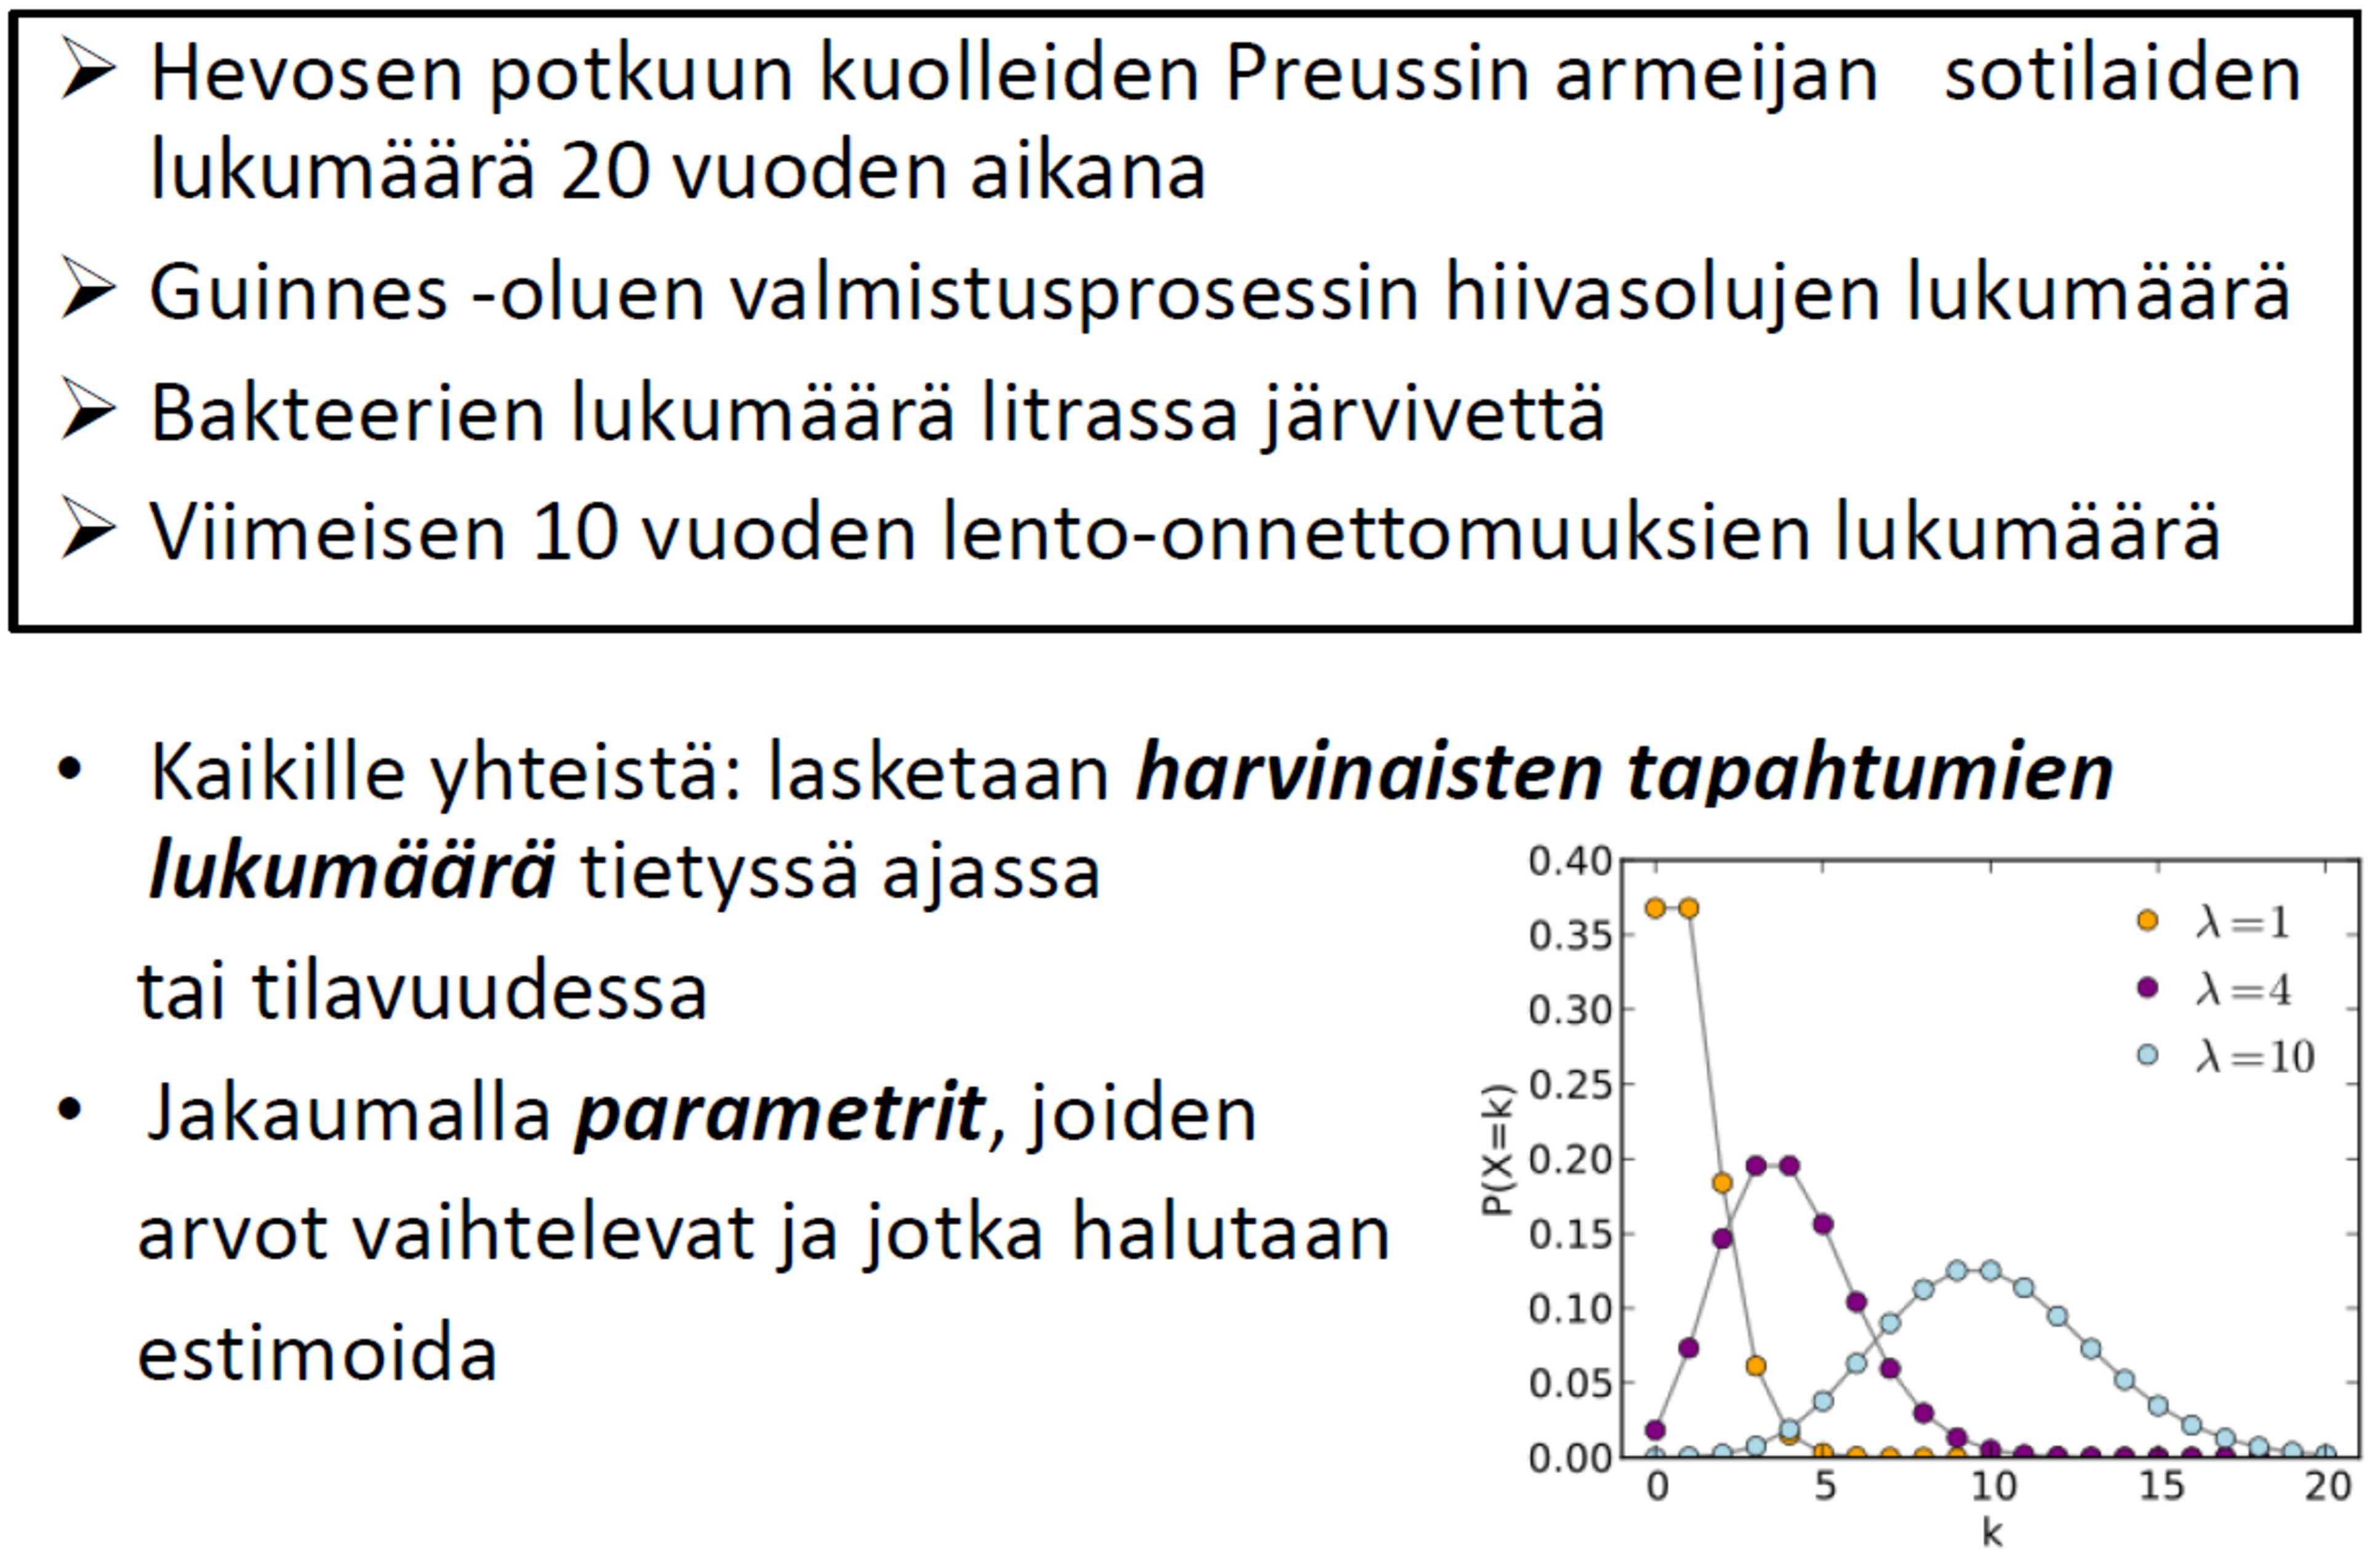
\includegraphics[width=1\linewidth]{images/poisson} 

}

\caption{Esimerkki: Poisson-jakauman sovelluskohteita ja sen pistetodennäköisyysfunktio eri parametrin $\lambda$ arvoilla.}\label{fig:poisson}
\end{figure}

\hfill\break

\textbf{Parametrien estimointi ja niiden testaus}

\begin{itemize}
\tightlist
\item
  Satunnaisilmiötä kuvaava tilastollinen malli perustuu siis johonkin parametriseen todennäköisyysjakaumaan, joka yhdessä havaintojen kanssa määrittää uskottavuusfunktion.

  \begin{itemize}
  \tightlist
  \item
    Aineistoa kuvaavan tilastollisen mallin uskottavuus pyritään maksimoimaan, mikä tarkoittaa valitun todennäköisyysjakauman sovittamista havaintoaineistoon mahdollisimman hyvin.
  \item
    Tässä nk. ``suurimman uskottavuuden estimoinnissa'' aineiston generoiman (oletetun) todennäköisyysjakauman parametriarvot \textbf{estimoidaan} (eli arvioidaan) käytettävän otoksen/aineiston avulla.
  \item
    Perusjoukkoa parhaiten kuvaavan (eli ``aineiston generoineen'') parametrin arvo pyritään siis estimoimaan aineiston perusteella.
  \end{itemize}
\item
  Parametrien estimoinnin lisäksi usein \textbf{testataan} parametreja koskevia oletuksia (eli hypoteeseja).
\item
  Estimointi ja testaus ovat tilastolliseen tutkimukseen liittyvän \textbf{tilastollisen päättelyn} keskeisiä välineitä, joiden avulla tutkittavasta ilmiöstä pyritään tekemään johtopäätöksiä siitä kerätyn havaintoaineiston perusteella.

  \begin{itemize}
  \tightlist
  \item
    Estimoitujen parametrien testaus voi vastata esimerkiksi seuraavanlaisiin kysymyksiin:

    \begin{itemize}
    \tightlist
    \item
      Onko suomalaisten miesten keskipituus 180~cm?
    \item
      Vaikuttaako yliopistokoulutus tulevaisuuden ansioihin?
    \item
      Auttaako tietty lääkeaine jonkin sairauden hoidossa?
    \item
      Voiko osakemarkkinoiden tuottoja ennustaa?
    \end{itemize}
  \end{itemize}
\item
  Parametrien testaus on osa tilastollista päättelyä, johon palataan tarkemmin luvussa \ref{luku6}
\end{itemize}

\hypertarget{alaluku44}{%
\section{Odotusarvo ja varianssi}\label{alaluku44}}

\begin{itemize}
\tightlist
\item
  Satunnaismuuttujan todennäköisyysjakauman tietoa voidaan tiivistää tunnuslukuihin, joista keskeisimpiä ovat \textbf{odotusarvo}, \textbf{varianssi} ja \textbf{keskihajonta}.
\end{itemize}

\begin{defblock}{}

\textbf{Odotusarvo}

Satunnaismuuttujan \(Y\) odotusarvo \(\text{E}(Y)\) kuvaa satunnaismuuttujan odotettavissa olevaa arvoa.

\begin{itemize}
\tightlist
\item
  Muodostamalla satunnaiskokeen tulosten \textbf{painotettu keskiarvo}, jossa kunkin tuloksen painona on vastaavan tapauksen todennäköisyys, niin saatua arvoa sanotaan odotusarvoksi \(\text{E}(Y)\).
\item
  Odotusarvo kuvaa jakauman painopistettä.
\item
  Merkinnän \(\text{E}(Y)\) käyttö juontaa juurensa englannin kielen sanoihin ``odotus'', expectation, ja ``odotusarvo'', expected value.
\end{itemize}

\end{defblock}

\newpage

\begin{eblock}{}
\textbf{Esimerkki: Odotusarvo}

Perinteikäs esimerkki odotusarvosta on tavallisen kuusitahoisen nopan silmäluvun odotusarvo. Nopanheitto on diskreetti satunnaisilmiö ja tavallisen painottamattoman nopan tapauksessa jokaisen silmäluvun todennäköisyys on yhtä suuri. Merkitään nopan silmälukua (sm) \(Y\) ja sen realisaatiota \(y\). Nopan silmäluvun realisaatioiden mahdolliset arvot ovat \(Y = \{1,2,3,4,5,6\}\) ja niiden todennäköisyydet ovat \(P(Y=y) = \frac{1}{6}\).

Nopanheiton silmäluvun odotusarvo määritetään siis painotettuna keskiarvona \[E(Y) = \sum_{i=1}^6 y \cdot P(Y=y)  = 1 \cdot \frac{1}{6} + 2 \cdot \frac{1}{6} + 3 \cdot \frac{1}{6} + 4 \cdot \frac{1}{6} + 5 \cdot \frac{1}{6} + 6 \cdot \frac{1}{6} = \frac{7}{2} = 3.5\]

\end{eblock}

\hfill\break

\begin{itemize}
\tightlist
\item
  Odotusarvon lisäksi kiinnostuksen kohteena on usein jakauman keskittyneisyys (hajaantuneisuus). Ts. kun halutaan puolestaan kuvata satunnaismuuttujan arvojen vaihtelua, tutkitaan todennäköisyysjakauman \textbf{varianssia} ja \textbf{keskihajontaa}.
\end{itemize}

\begin{defblock}{}

\textbf{Varianssi}

Satunnaismuuttujan \(Y\) hajontaa voidaan mitata varianssilla
\[
\mathrm{Var}(Y) = \text{E}\Big[\Big(Y-\text{E}(Y)\Big)^2\Big],
\]
tai sen neliöjuuren eli \textbf{keskihajonnan} avulla
\[
\text{D}(Y) = \sqrt{\mathrm{Var}(Y)}.
\]

\begin{itemize}
\tightlist
\item
  Mitä lähempänä nollaa keskihajonta ja varianssi ovat, sitä todennäköisempää on, että satunnaismuuttujan arvo on lähellä odotusarvoa.
\item
  Merkintöjen \(\mathrm{Var}(Y)\) ja \(\text{D}(Y)\) taustalla on englannin kielen sanat variance (varianssi) ja deviation, joka tarkoittaa ``poikkeamaa''/``hajontaa''.
\end{itemize}

\end{defblock}

\begin{itemize}
\tightlist
\item
  Odotusarvon ja varianssin (keskihajonnan) tavanomaiset \textbf{estimaattorit} ovat otoskeskiarvo ja otosvarianssi (otoshajonta), joihin palataan vielä myöhemmin.
\end{itemize}

\hypertarget{alaluku45}{%
\section{Joitain jakaumia}\label{alaluku45}}

Tarkastellaan seuraavassa muutamia keskeisiä tilastollisia jakaumia. Esittelemme ensin keskeisintä jatkuvien satunnaismuuttujien jakaumaa, normaalijakaumaa, ennen muutamien diskreettien satunnaismuuttujien jakaumia.

\hypertarget{normaalijakauma}{%
\subsection{Normaalijakauma}\label{normaalijakauma}}

\begin{itemize}
\item
  Jos satunnaismuuttuja \(Y\) noudattaa \textbf{normaalijakaumaa} odotusarvolla \(\text{E}(Y)= \mu\) ja varianssilla \(\mathrm{Var}(Y) = \sigma^2\), niin tällöin merkitään \(Y \thicksim \text{N}(\mu, \sigma^2)\).
\item
  \(Y\):n tiheysfunktio on muotoa (ks. kuva alla)
  \[
  f(y; \mu, \sigma^2) = \frac{1}{\sqrt{2 \pi \sigma^2}} \, e^{-\frac{1}{2} \Big(\frac{y- \mu}{\sigma} \Big)^2}, 
  \]
\end{itemize}

jossa \(e\) viittaa Neperin lukuun \(e \approx 2,71828\).

\begin{itemize}
\tightlist
\item
  Ylläoleva tiheysfunktio määrittelee parven normaalijakaumia kun parametreille (vakioille) \(\mu\) ja \(\sigma^2\) annetaan erilaisia arvoja. Nämä kaksi parametria määräävät normaalijakauman tarkemman muodon.

  \begin{itemize}
  \tightlist
  \item
    Alla olevassa kuvassa \ref{fig:normaalijakauma} on kuvattu erilaisia normaalijakauman tiheysfunktion muotoja eri parametriarvoille.
  \end{itemize}
\end{itemize}

\begin{figure}

{\centering 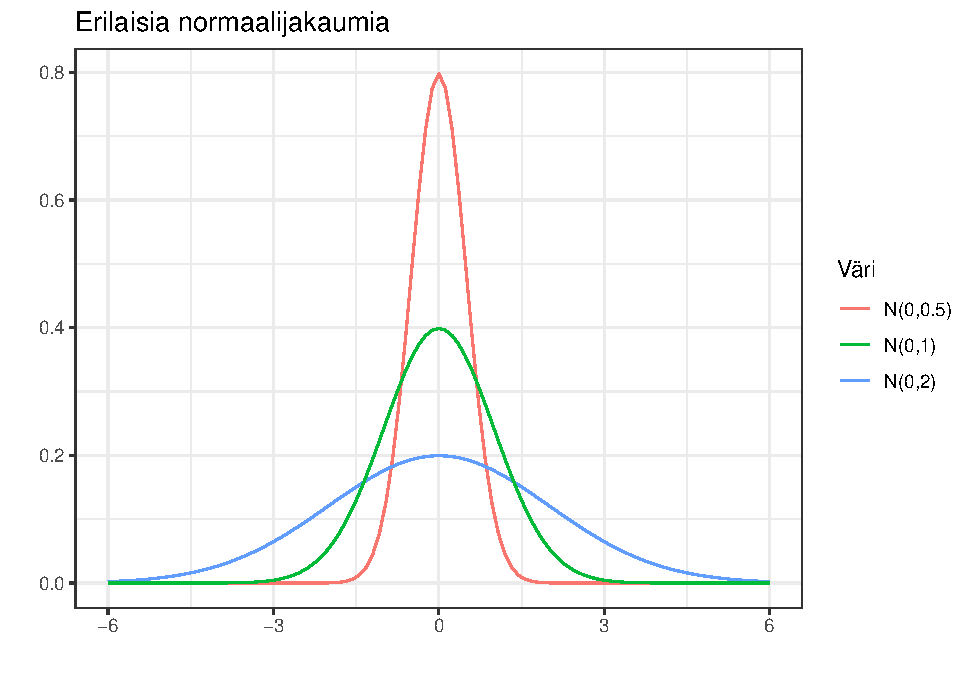
\includegraphics[width=1\linewidth]{TD2023_files/figure-latex/normaalijakauma-1} 

}

\caption{Normaalijakaumien muotoja eri parametriarvoilla.}\label{fig:normaalijakauma}
\end{figure}

\begin{eblock}{}

\textbf{Esimerkki: Miesten pituus}

\begin{itemize}
\tightlist
\item
  Tutkitaan miesten pituutta hyvin määritellyssä joukossa, kuten varusmiespalvelusta tiettynä vuonna suorittavien joukossa.

  \begin{itemize}
  \tightlist
  \item
    Pituus on ominaisuus, jonka voidaan nähdä määräytyvän monista perintö- ja ympäristötekijöistä. Pituutta voidaan siis pitää satunnaismuuttujana.
  \item
    Oletetaan, että pituus noudattaa normaalijakaumaa. Näin ollen sm. \(Y\) on valitun miehen pituus ja \(Y \thicksim \text{N}(\mu, \sigma^2)\).
  \end{itemize}
\item
  Tuntemattomien parametrien \(\mu\) ja \(\sigma^2\) tulkinta:

  \begin{itemize}
  \tightlist
  \item
    Odotusarvo \(\mu = \text{E}(Y)\) on satunnaisesti valitun miehen pituuden odotettavissa oleva arvo.
  \item
    Varianssi \(\sigma^2 = \mathrm{Var}(Y) = \text{E} \Big[\Big(Y- \mu \Big)^2 \Big]\) kuvaa valitun miehen pituuden odotusarvostaan määrätyn poikkeaman (keskihajonnan) neliön odotettavissa olevaa arvoa (kuvaten ts. pituuksien jakauman keskittyneisyyttä/hajaantuneisuutta pituuksien odotusarvon ympärillä).
  \end{itemize}
\end{itemize}

\end{eblock}

\hfill\break

\hypertarget{bernoulli--binomi--ja-poisson-jakauma}{%
\subsection{Bernoulli-, binomi- ja Poisson-jakauma}\label{bernoulli--binomi--ja-poisson-jakauma}}

\begin{itemize}
\tightlist
\item
  \textbf{Bernoulli-jakauma} on todennäköisyysjakauma, jossa satunnaismuuttujalla \(Y\) on kaksi mahdollista tulosvaihtoehtoa \(Y=1\) tai \(Y=0\).

  \begin{itemize}
  \tightlist
  \item
    Yleensä \(Y=0\) tarkoittaa, että jokin tapahtuma ei tapahdu ja \(Y=1\) että tapahtuu.
  \item
    Todennäköisyys tapahtumalle \(Y=1\) on \(\text{P}(Y=1)=p\) ja vastaavasti vastatodennäköisyys \(\text{P}(Y=0)=1-p\).
  \item
    Bernoulli-jakaumaa merkitään \(Y \thicksim B(p)\), jossa siis \(0 < p < 1\).
  \item
    Bernoulli-jakauman pistetodennäköisyysfunktio on muotoa
    \[
    f(y; p) = \text{P}(Y=y) = p^y (1-p)^{(1-y)},
    \]
    jossa \(y\) on sm:n \(Y\) realisaatio (havaittu arvo) ja parametri \(p\) on tuntematon (voidaan estimoida otoksen avulla, kuten myöhemmin tullaan näkemään).
  \end{itemize}
\item
  Bernoulli-jakauman odotusarvo \(\text{E}(Y)=p\) ja varianssi \(\mathrm{Var}(Y)=p (1-p)\).
\end{itemize}

\hfill\break

\begin{itemize}
\tightlist
\item
  \textbf{Binomijakauma}

  \begin{itemize}
  \tightlist
  \item
    Olkoon \(Y_1, \ldots, Y_n\) riippumattomia satunnaismuuttujia ja \(Y_i \thicksim B(p), \, i=1,\ldots,n\).
  \item
    Jos \(X = Y_1 + Y_2 + \ldots + Y_n\), niin \(X \thicksim \mathrm{Bin}(n,p)\). Ts. sm. \(X\) noudattaa \textbf{binomijakaumaa} parametrein \(n\) ja \(p\).
  \item
    Pistetodennäköisyysfunktio:
  \end{itemize}
\end{itemize}

\[
\text{P}(X=k) = \binom nk p^k (1-p)^{(n-k)}.
\]

\begin{itemize}
\tightlist
\item
  Jakauman odotusarvo \(\text{E}(X)=np\) ja varianssi \(\mathrm{Var}(X) = n p (1-p)\).
\item
  Binomijakaumalla kyetään vastaamaan mm. kysymykseen millä todennäköisyydellä \(n\):n kokoisessa otoksessa tapahtuu \(k\) onnistumista.
\end{itemize}

\begin{eblock}{}
\textbf{Esimerkki: Miesten lukumäärä Saksin osavaltion perheissä 1876--1885}\footnote{Ks. tarkemmin esimerkki 3.2 kirjassa (s. 67-68) Friendly, M., ja D. Meyer (2015). \emph{Discrete Data Analysis with R. Visualization and Modeling Techniques for Categorical and Count Data.} Chapman \& Hall/CRC.}

Vuosien 1876--1885 aikana Saksin osavaltiossa rekisteröitiin yli neljä miljoonaa syntynyttä lasta. Tällöin vanhempien tuli ilmoittaa lapsen sukupuoli (mies tai nainen) heidän syntymätodistuksessaan. Myöhemmässä tutkimuksessa tutkittiin tarkemmin 6115 perhettä, joissa asui 12 lasta ja tarkemmin miesten (poikien) lukumäärää näissä perheissä.

Oheisessa taulukossa taulukoidaan miesten (poikien) lukumäärät näissä 12 lapseen perheissä. Tarkasteltava jakauma esitetään vielä erikseen oheisessa kuviossa \ref{fig:miestenlkm}.

Tässä tilantessa mielenkiinnon kohteena saattaisi olla hypoteesi, jonka mukaan pojan (miehen) syntymätodennäköisyys \(\text{P}(\mathrm{mies}) = p\) on \(p=0.5\).

\end{eblock}

\FloatBarrier

\begin{table}
\centering\begingroup\fontsize{12}{14}\selectfont

\resizebox{\linewidth}{!}{
\begin{tabular}{lrrrrrrrrrrrrr}
\toprule
  & 0 & 1 & 2 & 3 & 4 & 5 & 6 & 7 & 8 & 9 & 10 & 11 & 12\\
\midrule
Miesten lkm & 0 & 1 & 2 & 3 & 4 & 5 & 6 & 7 & 8 & 9 & 10 & 11 & 12\\
Perheiden lkm & 3 & 24 & 104 & 286 & 670 & 1033 & 1343 & 1112 & 829 & 478 & 181 & 45 & 7\\
\bottomrule
\end{tabular}}
\endgroup{}
\end{table}

\FloatBarrier

\begin{figure}

{\centering 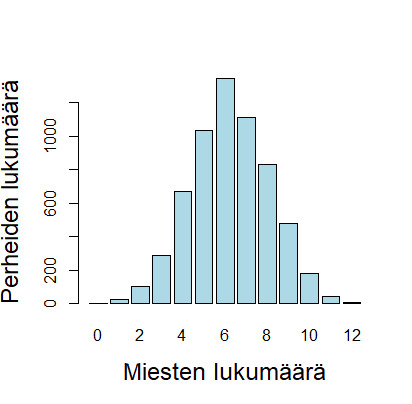
\includegraphics[width=7.5\linewidth]{images/Miesten_lkm} 

}

\caption{Miesten lukumäärä Saksin osavaltiossa 12:n lapsen perheissä.}\label{fig:miestenlkm}
\end{figure}

\FloatBarrier

\textbf{Poisson-jakauma}

\begin{itemize}
\item
  Jos satunnaismuuttuja \(Y\) on Poisson-jakautunut, merkitään \(Y \thicksim P(\lambda)\), jossa parametri \(\lambda > 0\) on Poisson-jakauman parametri, jota kutsutaan myös ajoittain intensiteettiparametriksi.
\item
  Poisson-jakaumaa voidaan käyttää tilanteissa, joissa sm. \(Y\) on jokin lukumäärä ja sen pistetodennäköisyysfunktio on muotoa
  \[
  \text{P}(Y=k) = \frac{e^{-\lambda} \lambda^k}{k!}.
  \]
\item
  Odotusarvo ja varianssi ovat Poisson-jakauman tapauksessa samat: \(\text{E}(Y) = \mathrm{Var}(Y) = \lambda\).
\end{itemize}

\begin{eblock}{}
\textbf{Esimerkki: Poisson-jakauma}

Tarkastellaan Englannin Valioliigakauden 1995--1996 otteluissa tehtyjä maalimääriä. Valioliiga (The F.A. Premier League) on korkein Englannin jalkapalloliigan sarjataso, jossa ensi kerran juuri kaudella 1995-1996 20 joukkuetta (aiemmin Valioliigan perustamisen kauden 1992--1993 alussa 22 joukkuetta) pelasivat keskenään kerran toisiaan vastaan koti- ja vieraskentällä. Otteluita oli siis yhteensä 380.

Tämä esimerkki perustuu edellä mainittuun Friendlyn ja Meyerin (2015) kirjan esimerkkiin 3.9 (s. 78-79), joka vastaavasti perustuu Alan J. Leen (1997) artikkeliin\footnote{Alan J. Lee (1997). Modeling Scores in the Premier League: Is Manchester United Really the Best? \emph{Chance} 10(1), 15-19.}, jonka esittämään kysymykseen (hypoteesiin) vastaus on tietenkin ilmeinen! Näin ollen seuraavassa tarkastellaankin kotijoukkueiden ja vierasjoukkueiden maalintekointensiteettiä Poisson-jakaumaan perustuen. Seuraavassa emme siis pyri mallintamaan tietyn spesifin ottelun lopputulosta vaan tarkastelemme ``keskimääräisen'' kotijoukkueen ja vierasjoukkueen ``edustavaa'' ottelua.

Seuraava taulukko raportoi tehtyjen maalimäärien jakaumat pelatuissa 380 ottelussa. Neljän tai yli neljän maalin tapaukset kirjataan 4+:nä maalina. Ts. esim. kys. kauden lopputulokset \emph{Blackburn Rovers} - \emph{Nottingham Forest} 7-0 ja \emph{Bolton Wanderers} - \emph{Manchester United} 0-6 tulevat aineistoon tuloksina 4+ vs.~0 ja 0 vs.~4+.

\end{eblock}

\begin{tabular}{lrrrrrr}
\toprule
\multicolumn{1}{c}{Kotij. maalien lkm.} & \multicolumn{5}{c}{Vierasj. maalien lkm.} & \multicolumn{1}{c}{Yht.} \\
\cmidrule(l{3pt}r{3pt}){1-1} \cmidrule(l{3pt}r{3pt}){2-6} \cmidrule(l{3pt}r{3pt}){7-7}
  & 0 & 1 & 2 & 3 & 4+ & Yht.\\
\midrule
0 & 27 & 29 & 10 & 8 & 2 & 76\\
1 & 59 & 53 & 14 & 12 & 4 & 142\\
2 & 28 & 32 & 14 & 12 & 4 & 90\\
3 & 19 & 14 & 7 & 4 & 1 & 45\\
4+ & 7 & 8 & 10 & 2 & 0 & 27\\
\addlinespace
Yht. & 140 & 136 & 55 & 38 & 11 & 380\\
\bottomrule
\end{tabular}

\begin{eblock}{}
\textbf{Esimerkki (jatkuu): Poisson-jakauma}

Olettamalla, että koti- ja vierasjoukkueen todennäköisyys tehdä maali ottelun aikana on vakio, niin tällöin koti- ja vierasjoukkueen ottelun aikana tekemien maalien lukumäärää (ilman edellä käytettyä maalimäärien ``katkaisua'' neljään) voidaan melko hyvin approksimoida oletuksella, että nämä lukumäärät ovat Poisson-jakautuneita. Ts. \(Y^H_i \thicksim P(\lambda_H)\) on sm., joka kuvaa \(i\):n ottelun kotijoukkueen tekemien maalien lukumäärää ja intensiteettiparametrin \(\lambda_H\) arvon määrittäminen kuuluu tilastollisen päättelyn ja erityisesti estimointiteorian piiriin. Vastaavasti vierasjoukkueen maalimäärät: \(Y^A_i \thicksim P(\lambda_A)\).

Osoittautuu, että parametreille \(\lambda_H\) ja \(\lambda_A\) saatavat estimaatit ovat \(\lambda_H = 1.49\) ja \(\lambda_A = 1.06\) ja ne vastaavat tässä yksinkertaistetussa tilanteessa koti- ja vierasjoukkueen keskimääräisiä maalimääriä:

\end{eblock}

\FloatBarrier

\begin{tabular}{llll}
\toprule
  & Kotijoukkue (home) & Vierasjoukkue (away) & Yht.\\
\midrule
Keskiarvo & 1.486 & 1.063 & 2.550\\
Varianssi & 1.316 & 1.172 & 2.618\\
\bottomrule
\end{tabular}

\begin{eblock}{}
Tuloksista voidaan siis päätellä, että kotijoukkueen (odotettavissa oleva) maalimäärä on vierasjoukkuetta korkeampi (osoittaen kotiedun merkitystä jalkapallossa). Lisäksi edellä todetun Poisson-jakauman teoreettisten ominaisuuksien mukaisesti keskimääräiset maalimäärät ovat lähellä niiden variansseja, mikä osoittaa osaltaan (tässä yksinkertaistetussa tilanteessa), että Poisson-jakaumaan perustuva jakaumaoletus on kelvollinen.

On syytä todeta lopuksi, että tämän vahvasti yksinkertaistetun tilanteen sijaan tilastotieteessä on laaja ja kasvava kirjallisuuden haara jalkapalloa ja muuta urheilua koskevien tilastollisen menetelmien saralla. Nämä vaativat kuitenkin syvällisemmän ymmärryksen saavuttamiseksi jälleen huomattavasti laajempia tilastotieteen (aine- ja syventäviä) opintoja.

\end{eblock}

\hypertarget{alaluku46}{%
\section{Sattuman rooli tieteenteossa: Vale-emävale-tilasto?}\label{alaluku46}}

Erityisesti nykypäivänä ei-tieteellinen tieto ja tarkoituksellinen disinformaatio, joita perustellaan heppoisin havainnoin, leviävät internetissä kulovalkean tavoin. On tiedeyhteisön ja tutkijoiden moraalinen vastuu taistella näitä uskomuksia vastaan \textbf{popularisoimalla tiedettä}. Tämä saattaa kuitenkin ajoittain jopa pahentaa ongelmaa, sillä popularisoinnissa päteviltäkin tutkijoilta voi unohtua \emph{satunnaisuuden voima}.\footnote{~Tämä jakso perustuu osin psykometriikan yliopisto-opettajan Jari Lipsasen \href{https://blogs.helsinki.fi/med-viikonjuttu/2021/02/22/vale-emavale-tilasto}{blogiin} vuodelta 2021.}

\begin{itemize}
\tightlist
\item
  Kuten todettua, tilastollisessa tutkimuksessa mielenkiinnon kohteena on satunnaisilmiöiden tutkiminen ja erityisesti systemaattisen ja satunnaisen vaihtelun (signaalin ja kohinan) erottaminen sekä muuttujien välisten riippuvuuksien tutkiminen.

  \begin{itemize}
  \tightlist
  \item
    Kiinnostuksen kohteena on siis hyvin harvoin vain jokin yksittäinen tunnusluku, kuten keskiarvo, varianssi tai korrelaatio (palaamme näihin myöhemmin luvussa \ref{luku6}).
  \item
    Tieteen popularisointi on yksi tutkijoiden ja yliopistojen tiedeyhteisön tärkeimmistä yhteiskunnallisista tehtävistä, mutta valitettavan usein se typistyy yksittäisen viimeisimmän tutkimustuloksen esittelyksi.
  \end{itemize}
\item
  Yliopistoyhteisössä kuitenkin luonnollisesti luotamme kumuloituneeseen tutkittuun tietoon ja tiedämme, että \textbf{yksittäinen tutkimus on vasta hyvä alku}.

  \begin{itemize}
  \tightlist
  \item
    Ihmistieteitä, kuten ilmeisesti erityisesti psykologiaa sekä osin myös muiden ohella lääke- ja taloustiedettä, on viimeisen vuosikymmenen ajan puhuttanut paljon niin sanottu \textbf{replikaatiokriisi}, sillä useaa arvostettuakaan tutkimusta ei ole saatu \textbf{toistettua eli replikoitua}.
  \item
    On ymmärrettävää, että replikaatiokriisi, varsinkin jos se on (alakohtaisesti) laajalle levinnyttä, murentaa kansalaisten luottamusta tieteellisiin tuloksiin.
  \item
    Toistettavuus on yksi tutkimuksen peruskriteereistä, joka erottaa tieteellisen tiedon muista tietolähteistä, joten sen puuttuminen herättää ymmärrettävästi huolta tieteellisen prosessin toimivuudesta.
  \item
    Replikaatiokriisin voi kuitenkin myös tulkita toisin: ilman kriittisyyttä omia (ja muiden) tuloksia kohtaan, ei mitään kriisiä olisikaan, joten silkka sen olemassaolo on osoitus tieteellisen prosessin toimivuudesta.
  \end{itemize}
\item
  Kun tuntee ja tunnistaa sattuman voiman ja ymmärtää kaikki mahdolliset satunnaisuuden lähteet, jotka altistavat tutkimusprosessin virheille, tulee samalla ymmärtäneeksi että eri tavoin koeteltu, useassa tutkimuksessa kumuloitunut tieto tulisi olla kaiken tieteen popularisoinnin keskiössä yksittäisten, mahdollisesti uusien ja yllättävien tutkimustulosten sijaan.

  \begin{itemize}
  \tightlist
  \item
    Tähän mennessä olemme jo oppineet, että tälle on myös vahvat tilastolliset perustelut: satunnaisen tiedon maailmassa mikään ei ole täysin varmaa, ei edes kaikkein edistyneimpien tilastomenetelmien avulla!
  \end{itemize}
\end{itemize}

\hypertarget{luvun-4-yhteenveto-keskeisiuxe4-termejuxe4-ja-kokonaisuuksia.}{%
\section{Luvun 4 yhteenveto, keskeisiä termejä ja kokonaisuuksia.}\label{luvun-4-yhteenveto-keskeisiuxe4-termejuxe4-ja-kokonaisuuksia.}}

\begin{itemize}
\tightlist
\item
  Satunnaisilmiö
\item
  Satunnaismuuttuja
\item
  Jatkuvat ja diskreetit satunnaismuuttujat ja niihin liittyvät pistetodennäköisyysfunktio ja tiheysfunktio
\item
  Todennäköisyysjakauma
\item
  Tilastollinen malli (todennäköisyysmalli)
\item
  Kvalitatiiviset ja kvantitatiiviset muuttujat
\item
  Frekventistinen ja Bayesiläinen tilastotiede
\item
  Odotusarvo ja varianssi
\item
  Yleisempiä jakaumia: Normaalijakauma, Bernoulli-jakauma, binomijakauma ja Poisson-jakauma
\item
  Tieteen popularisointi ja sen suhde (yksittäiseen) tutkimukseen
\end{itemize}

\hypertarget{luku5}{%
\chapter{Tilastolliset aineistot, niiden kerääminen ja mittaaminen}\label{luku5}}

Edellisessä luvussa käsiteltiin tilastotieteen suhtautumista satunnaisilmiöihin. Tässä luvussa tarkastelemme lähemmin miten reaalimaailman satunnaisilmiöistä kerätään tietoa ja miten niitä voidaan mitata. Tilastotieteen perusoppimäärä rakentuu ajatukselle ilmiöiden tutkimisesta rajallisen ja epävarman tiedon vallitessa. Käytännössä tämä tarkoittaa sitä, että tutkimuksen kohteena olevat rajalliset aineistot sisältävät niin systemaattista kuin satunnaisuudesta johtuvaa vaihtelua. Tilastollisten menetelmien avulla pyrimme erottamaan systemaattisen vaihtelun satunnaisesta sekä tekemään tilastollista päättelyä aineiston generoimasta mekanismista. Lyhyesti tämä tarkoittaa aineiston systemaattisen vaihtelun tilastollista mallintamista ja sen parametrien estimointia otoksesta, joka kattaa vain (pienen) osajoukon koko populaation (perusjoukon) tilastoyksiköistä.

Voidaksemme tehdä uskottavaa päättelyä ``havainnoista parametreihin'', tulee otoksen olla riittävän \textbf{edustava}. Tämän luvun keskeisin oppi onkin, että miten \textbf{otanta} tulisi suorittaa, jotta havaintoaineisto olisi \textbf{edustava otos} populaatiosta, silloin kun aineisto kerätään otannalla. Vaikka aineiston hankinta vaatii yleensä runsaasti käytännön työtä, kannattaa se tehdä huolellisesti, sillä huonosti toteutetun otannan vuoksi tutkimusongelman kannalta keskeisiä johtopäätöksiä ei voida tehdä!

\hypertarget{alaluku51}{%
\section{Kertausta: Data eli aineisto}\label{alaluku51}}

\begin{itemize}
\tightlist
\item
  \textbf{Tilastollinen tutkimus} aloitetaan tutkimusaineiston keruun suunnittelulla.
\item
  Kertauksen vuoksi: tilastollinen tutkimusaineisto (havaintoaineisto) koostuu tilastoyksiköiden populaatiosta havaituista tilastomuuttujien arvoista.
\end{itemize}

\begin{figure}
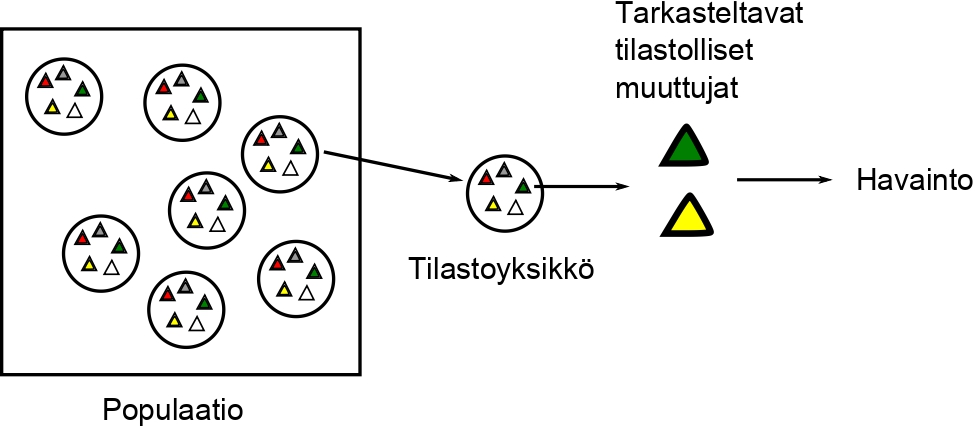
\includegraphics[width=0.9\linewidth]{images/populaatiostahavaintoon} \caption{Populaatiosta havaintoon.}\label{fig:pophav}
\end{figure}

\begin{itemize}
\tightlist
\item
  Havaintoaineisto voidaan koota taulukoksi, johon listataan tilastoyksiköt riveille ja tilastomuuttujat sarakkeisiin. Jos havaintoaineisto koostuu \(n\) tilastoyksiköstä, joista jokaisesta on kerätty esim. \(m\):stä tilastomuuttujasta havainnot, niin aineisto voidaan kirjoittaa taulukon muotoon:
\end{itemize}

\begin{longtable}[]{@{}
  >{\raggedright\arraybackslash}p{(\columnwidth - 8\tabcolsep) * \real{0.2326}}
  >{\raggedright\arraybackslash}p{(\columnwidth - 8\tabcolsep) * \real{0.2326}}
  >{\raggedright\arraybackslash}p{(\columnwidth - 8\tabcolsep) * \real{0.2326}}
  >{\raggedright\arraybackslash}p{(\columnwidth - 8\tabcolsep) * \real{0.0698}}
  >{\raggedright\arraybackslash}p{(\columnwidth - 8\tabcolsep) * \real{0.2326}}@{}}
\toprule\noalign{}
\begin{minipage}[b]{\linewidth}\raggedright
\end{minipage} & \begin{minipage}[b]{\linewidth}\raggedright
tilastomuuttuja 1
\end{minipage} & \begin{minipage}[b]{\linewidth}\raggedright
tilastomuuttuja 2
\end{minipage} & \begin{minipage}[b]{\linewidth}\raggedright
\(\dots\)
\end{minipage} & \begin{minipage}[b]{\linewidth}\raggedright
tilastomuuttuja \(m\)
\end{minipage} \\
\midrule\noalign{}
\endhead
\bottomrule\noalign{}
\endlastfoot
tilastoyksikkö 1 & \(x_{1,1}\) & \(x_{1,2}\) & \(\dots\) & \(x_{1,m}\) \\
tilastoyksikkö 2 & \(x_{2,2}\) & \(x_{2,2}\) & \(\dots\) & \(x_{2,m}\) \\
\(\vdots\) & \(\vdots\) & \(\vdots\) & & \(\vdots\) \\
tilastoyksikkö \(n\) & \(x_{n,1}\) & \(x_{1,2}\) & \(\dots\) & \(x_{n,m}\) \\
\end{longtable}

Tässä siis rivillä \(i\) on \(i\). \textbf{tilastoyksikön} havainto ja sarakkeessa \(j\) on \(j\). tilastollisesta muuttujasta havaitut arvot \(x_{i,j}\). Ts. yhdellä rivillä on yhden tilastoyksikön tiedot kaikista tilastomuuttujista ja yksi sarake on kaikkien tilastoyksiköiden tiedot yhdestä tilastomuuttujasta.

\begin{itemize}
\tightlist
\item
  Usein (varsinkin parhaillaan kiihtyvällä vauhdilla) kerättävät havaintoaineistot ovat niin suuria, ettei edellisenkaltaisesta havaintotaulukosta voida usein suoraan tarkastelemalla nähdä aineiston pääpiirteitä.

  \begin{itemize}
  \tightlist
  \item
    Tällöin voi olla tarpeen luokitella aineistoa taulukon muodostamiseksi.\\
  \item
    Luokittelussa on kysymys aineiston tiivistämisestä kohtuullisen kokoiseksi ja havainnollisempaan muotoon. Luokittelussa tilastomuuttujan arvot sijoitetaan eri luokkiin siten, että yhden tilastomuuttujan arvo voi kuulua vain yhteen luokkaan. Luokka ilmoitetaan yleensä luokkavälinä, kuten reaalilukuvälinä. Esimerkiksi henkilön ikä on tapana luokitella ikäjakauman kuvaamisessa 10-vuotisluokkiin (15-24, 25-34, \ldots), vaikka periaatteessa ikä voitaisiin ilmoittaa minuutinkin tarkkuudella.\\
  \item
    Luokkien lukumäärään vaikuttavat muun muassa tilastomuuttujan arvojen vaihteluväli ja havaintoaineiston laajuus. Luokittelussa pyritään siihen, että luokkien lukumäärä saadaan tarvittaessa luokkia yhdistämällä kohtuulliseksi ja että luokat valitaan tasavälisesti eli siten, että kahden peräkkäisen luokan alarajojen erotus on vakio. Kun aineistoa luokitellaan, aineiston luettavuus paranee mutta toisaalta osa tiedoista menetetään eivätkä yksittäiset havaintoarvot ole enää tiedossa.\\
  \item
    Emme vielä tällä kurssilla käsittele tilastografiikan esittämistä tarkemmin. Muun muassa tilastollisen päättelyn peruskurssi (TILM3555) vastaa näihin kysymyksiin tarkemmin. Graafiset menetelmät ovat joka tapauksessa erittäin tärkeä osa aineiston havainnollistamista. Kuvat helpottavat aineiston tulkitsemista ja toimivat usein perusteltuna lähtökohtana monimutkaisempien tilastollisten mallien (ja algoritmien) sovittamiselle.
  \end{itemize}
\end{itemize}

\hfill\break

\begin{itemize}
\tightlist
\item
  Kvantitatiivisen tutkimuksen aineistoksi kelpaa periaatteessa kaikki havaintoihin perustuva informaatio, joka on \textbf{mittauksen} avulla muutettavissa numeeriseen muotoon.

  \begin{itemize}
  \tightlist
  \item
    Havaintoyksiköiden tilastollisten muuttujien numeerisia arvoja kutsutaan \textbf{havaintoarvoiksi} tai \textbf{havainnoiksi}.
  \item
    Kaikki havaitut tilastolliset muuttujat eivät ole aina mielenkiintoisia. Tutkimuksen kannalta mielenkiintoisia muuttujia kutsutaan \textbf{tutkimusmuuttujiksi}, joiden lisäksi havaintoaineisto pitää mahdollisesti sisällään \textbf{taustamuuttujia}.

    \begin{itemize}
    \tightlist
    \item
      Esimerkiksi, jos tutkimuksella halutaan tietoa suomalaisen aikuisväestön mielipiteistä, havaintoyksikköinä ovat aikuisväestöön kuuluvat henkilöt. Jos halutaan tietoa suomalaisista kunnista, havaintoyksikköinä ovat Suomen kunnat jne.
    \item
      Ensimmäisessä tapauksessa tilastollisina muuttujina on aikuisväestön mielipiteet, joita voidaan selvittää esimerkiksi kyselytutkimuksella. Toisaalta voidaan myös kerätä taustamuuttujiksi haastatelluista muita tietoja, kuten asuinpaikka, ikä ja ammatti.
    \end{itemize}
  \item
    Kaikkia mielenkiintoisia muuttujia ei kuitenkaan välttämättä voida havaita, eli niille ei voida määrittää numeerista arvoa. Tällöin puhutaan nk. \textbf{latenteista muuttujista}, eli muuttujista joita ei suoraan havaita mutta joiden oletetaan vaikuttavan havaittavien muuttujien taustalla. Latentteja muuttujia voidaan rakentaa tilastollisten mallien avulla käyttäen hyödyksi niihin liittyviä havaittuja muuttujia.

    \begin{itemize}
    \tightlist
    \item
      Latentteja muuttujia ovat esimerkiksi elämänlaatu, onnellisuus, konservatiivisuus, yms.
    \end{itemize}
  \end{itemize}
\end{itemize}

\hfill\break

\begin{itemize}
\tightlist
\item
  Tilastollinen tutkimus voi olla joko \textbf{kokonaistutkimus} tai \textbf{otantatutkimus}.
\end{itemize}

\begin{defblock}{}

\textbf{Kokonaistutkimus}

Kokonaistutkimus on tutkimus, jossa tutkitaan kaikki tutkimuksen kohteena olevan perusjoukon alkiot, ts. kaikki ajateltavissa olevat kohteet tutkitaan.

\begin{itemize}
\tightlist
\item
  Kokonaistutkimus on yleinen tutkimustapa silloin, kun kohdeperusjoukko on selvästi määritelty ja sen alkioita koskevat tilastolliset muuttujat ovat helposti mitattavissa.
\item
  Esimerkiksi, jos tutkitaan Suomen kuntia, niin kokonaistutkimuksessa tutkitaan kaikki kunnat. Kunnista on useimmissa tilanteissa mahdollista kerätä mielenkiinnon kohteena olevia tilastollisia muuttujia.
\item
  Toisaalta, jos tutkitaan jonkin lääkeaineen vaikutuksia ihmisiin, niin kokonaistutkimuksessa tutkittaisiin jokainen ihminen erikseen. Selvää on, että tällainen kokonaistutkimus olisi liian vaikeaa toteuttaa.
\end{itemize}

\end{defblock}

\begin{defblock}{}

\textbf{Otantatutkimus}

Otantatutkimuksessa tutkimus kohdistetaan johonkin (populaation/perusjoukon) osajoukkoon, joka poimitaan sopivaa \textbf{otantamenetelmää} käyttäen (ks. alaluku \ref{alaluku55}) ja populaatiota/perusjoukkoa koskevat johtopäätelmät tehdään tähän otokseen perustuen.

\begin{itemize}
\tightlist
\item
  Otantatutkimus on usein luonnollinen valinta, sillä koko populaation tutkiminen ei useinkaan ole mahdollista tai kannattavaa.

  \begin{itemize}
  \tightlist
  \item
    Esimerkiksi aseiden patruunoita valmistava tehtailija ei voi tutkia toimivatko kaikki ammukset. Myöskään valaisimien valmistaja tuskin tekee kokonaistutkimuksia valmistamiensa tuotteiden kestoajan selvittämiseksi.\\
  \end{itemize}
\item
  Perusjoukosta otokseen poimittuja alkioita kutsutaan \textbf{otosyksiköiksi} ja niiden muodostama osajoukko, eli \textbf{otos}, on se osa perusjoukkoa, joka tutkitaan tutkimusaineiston keräämisen jälkeen.

  \begin{itemize}
  \tightlist
  \item
    Lääketutkimusta tehdäänkin poikkeuksetta otantatutkimuksena (ja kontrolloituina kokeina, ks. alempaa), jolloin lääkettä testataan vain osajoukolla koko ihmispopulaatiosta ja tämän osajoukon alkiot ovat otosyksiköitä.
  \item
    Näin toimimalla, ja riittävän edustavalla otoksella, saadaan kuitenkin tarpeeksi tietoa lääkeaineen vaikutuksista ja tulokset voidaan yleistää populaatiotasolle ja lääke ottaa käyttöön.
  \end{itemize}
\item
  Otantatutkimus on halvempi kuin kokonaistutkimus ja tulokset saadaan nopeammin!
\end{itemize}

\end{defblock}

\hfill\break

\begin{itemize}
\tightlist
\item
  Otantatutkimuksessa keskitytään siis perusjoukkoa edustavan pienemmän, mieluusti satunnaisesti valitun otoksen tutkimiseen.

  \begin{itemize}
  \tightlist
  \item
    Otantatutkimuksissa tiedot kerätään useimmiten haastattelemella, kirjallisella/sähköisellä kyselyllä tai suoraan tietorekistereistä. Tiedonkeruun toteuttaminen (eri sovelluksissa) määrää osaltaan käytettävän otantamenetelmän.
  \item
    Teoriassa äärelliseen perusjoukkoon kohdistuvat kokonaistutkimukset voidaan aina tulkita otantatutkimuksiksi (perusjoukko tulkitaan otokseksi hypoteettisesta äärettömästä perusjoukosta)!

    \begin{itemize}
    \tightlist
    \item
      Esimerkiksi Galilein tekemät painovoiman vaikutusta kappaleiden putoamisaikaan liittyneet mittaukset. Koetuloksia (mittauksia) voidaan pitää otoksena äärettömästä mahdollisten koetulosten joukosta. Tällöin ainoa mahdollisuus ilmiön tutkimiseen on käyttää otantaa.
    \end{itemize}
  \end{itemize}
\item
  Otantatutkimuksen tulokset voivat olla luotettavampia kuin kokonaistutkimuksen.

  \begin{itemize}
  \tightlist
  \item
    Otantatutkimuksessa voidaan panostaa enemmän huolelliseen ja tarkkaan mittaamiseen sekä valitun otoksen tavoittamiseen.
  \item
    Kokonaistutkimuksessa vastauskato ja tarkasteltavan populaation valintavirhe ovat mahdollisia siinä missä otantatutkimuksessakin.
  \end{itemize}
\item
  Otantateoria on yksi tilastotieteen keskeisimpiä oppeja ja tarjoaa teoreettisen kehikon empiiristen tutkimusten tulosten yleistämiseen. Tarkastellaan siis tarkemmin otannan ideaa ja toteuttamista seuraavassa alaluvussa.
\end{itemize}

\hypertarget{alaluku52}{%
\section{Otannan idea}\label{alaluku52}}

\begin{itemize}
\tightlist
\item
  Otantatutkimuksen (karkeat) suunnittelu- ja työvaiheet ovat seuraavat:

  \begin{enumerate}
  \def\labelenumi{\arabic{enumi}.}
  \tightlist
  \item
    Tavoitteiden asettaminen
  \item
    Perusjoukon (populaation) asettaminen
  \item
    Kehikko
  \item
    Kerättävän informaation sisältö (mitä tietoa todella tarvitaan, mitä voidaan jättää pois, suunnitellaan kysymykset ja mahdollinen kyselylomake)
  \item
    Otoskoon määrittäminen
  \item
    Suoritetaan otoksen poiminta, tietojen keräys ja tarkastus
  \item
    Aineiston taulukointi ja analysointi
  \item
    Raportin laatiminen
  \end{enumerate}
\item
  Otantatutkimuksessa ajatuksena on siis poimia \textbf{edustava otos} siitä populaatiosta (perusjoukosta), joka on mielenkiinnon kohteena eli jota halutaan tutkia ja josta halutaan tietoja.

  \begin{itemize}
  \tightlist
  \item
    \textbf{Tavoiteperusjoukko} on joukko, johon otannan myötä saatavat tutkimustulokset halutaan yleistää. Toisin sanoen, se mistä haluamme tietoja määrää populaation.
  \item
    \textbf{Kohdeperusjoukko} on joukko, jota koskevia tietoja halutaan kerätä.

    \begin{itemize}
    \tightlist
    \item
      Esimerkiksi äänestysikäiset Suomen kansalaiset.
    \item
      Usein tavoiteperusjoukko = kohdeperusjoukko.
    \item
      Tavoiteperusjoukko voi joskus olla laajempi (esim. ``ihmiset'' vs.~``suomalaiset'').
    \end{itemize}
  \end{itemize}
\item
  Tutkimuksessa (edustavaan) otokseen poimitut tilastoyksiköt, näiden tilastolliset muuttujat ja niiden arvot muodostavat \textbf{otosaineiston} eli siis tutkimus- tai havaintoaineiston (\textbf{datan}).

  \begin{itemize}
  \tightlist
  \item
    Tutkimuskysymykseen vastatakseen tutkija valitsee sopivan tilastollisen mallin ja estimoi sen parametrit tähän otokseen perustuen.
  \item
    Perusoletuksena on otoksen ja valitun tilastollisten mallin pohjalta suoritettavan tilastollisen päättelyn \textbf{yleistettävyys koko populaatioon}.
  \item
    Otos valitaan erilaisia \textbf{otantamenetelmiä} hyödyntäen pyrkien varmistamaan otoksen \textbf{edustavuus} (perusjoukko pienoiskoossa, ks. kuva \ref{fig:otanta}).
  \end{itemize}
\end{itemize}

\begin{defblock}{}
\textbf{Edustavuus}

Tutkimukseen valitut yksiköt edustavat koko populaatiota, ts. tutkimukseen valittu osajoukko kuvaa perusjoukon ominaisuuksia kattavasti.

\end{defblock}

\begin{itemize}
\tightlist
\item
  Keskeistä tutkimuksen ja sen edustavuuden kannalta on, että tutkija osaa kerätä sisällöllisesti ja määrällisesti \textbf{sopivan kokoisen} aineiston.
\item
  Tietyn otoksen edustavuutta arvioidessa voidaan käyttää apuna seuraavia kysymyksiä:

  \begin{itemize}
  \tightlist
  \item
    Miksi päädyttiin tämän kokoiseen otokseen?

    \begin{itemize}
    \tightlist
    \item
      \textbf{Otoskoko} vaikuttaa siihen miten hyvin otoksesta tehdyt johtopäätökset voidaan yleistää koskemaan koko perusjoukkoa, ts. kuinka luotettavia ne ovat. Tämä johtuu siitä, että yksittäisten otosyksiköiden ominaisuudet saattavat vaihdella suuresti ja kasvattamalla otoskokoa perusjoukon systemaattiset piirteet tulevat otoskoon kasvaessa yhä paremmin esille. Kun otoskoko vastaa populaation kokoa, on kyseessä tietenkin kokonaistutkimus, joka kertoo kaiken perusjoukosta. Otoskoon valintaan ja määräämiseen palataan myöhemmin luvussa \ref{luku6}.
    \end{itemize}
  \item
    Käytettiinkö apuna tilastotieteellisesti vankkaa suunnittelua otoskoon määrittämiseksi ja/tai miten pyrittiin varmistamaan tärkeisiin analyysiryhmiin kuuluvien riittävä määrä aineistossa?
  \item
    Harkittiinko muita otantamenetelmiä ja miksi päädyttiin juuri käytössä olleeseen menetelmään?
  \end{itemize}
\item
  Edustavuuteen vaikuttaa keskeisesti se, millä tavoin otanta pystytään suorittamaan, ts. mihin kohdeperusjoukkoon otanta kohdistetaan.

  \begin{itemize}
  \tightlist
  \item
    \textbf{Kehikkoperusjoukko} on rekisterin, luettelon tms. peittämä osa kohdeperusjoukkoa. Kyseessä on siis se osa kohdeperusjoukkoa, josta otanta ylipäänsä pystytään suorittamaan eli \textbf{otantakehikko}.
  \item
    \textbf{Otantakehikon alipeitto} esiintyy, kun otantakehikosta puuttuu osa kohdeperusjoukon alkioista (esim. tutkimus suoritetaan puhelinhaastattelulla, mutta osa aiottuun otokseen kuuluvista haastateltavista ei omista puhelinta). Vastaavasti \textbf{otantakehikon ylipeittoa} esiintyy, kun otantakehikkoon kuuluu kohdeperusjoukkoon kuulumattomia alkioita.

    \begin{itemize}
    \tightlist
    \item
      Nämä ovat nk. \textbf{kehikkovirheitä}. Lisäksi esimerkiksi kyselytutkimuksissa tai rekisteriaineistoissa saattaa esiintyä \textbf{katoa}, eli osa vastauksista jää uupumaan tai niitä ei jostain syystä mitata.
    \item
      \textbf{Otantavirhe} taas on satunnaisuudesta johtuvaa tilastollisten muuttujien vaihtelua otoksesta toiseen ja se onkin ainoa virhelaji, jonka suuruutta voidaan tilastollisin menetelmin arvioida.
    \end{itemize}
  \end{itemize}
\end{itemize}

\begin{figure}

{\centering 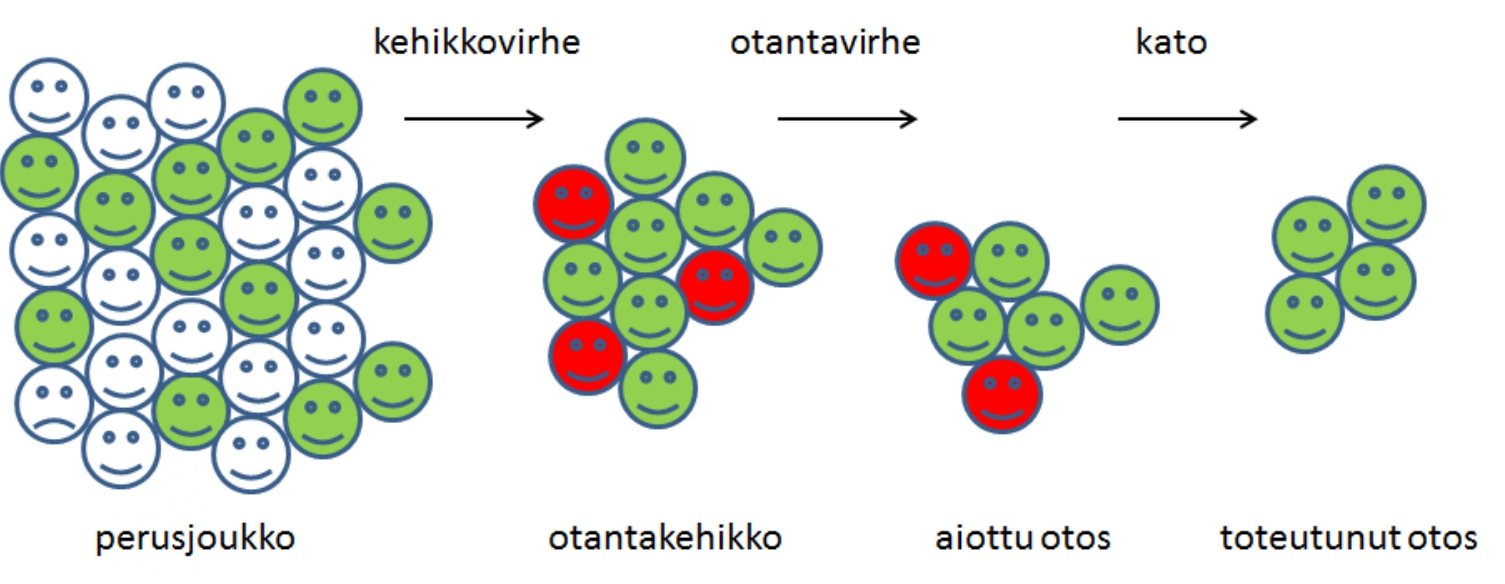
\includegraphics[width=1\linewidth]{images/otanta} 

}

\caption{Otannan idea.}\label{fig:otanta}
\end{figure}

\begin{itemize}
\tightlist
\item
  Edustavan otoksen avulla on mahdollista tehdä perusjoukkoa koskevaa tilastollista päättelyä, sillä otos kuvaa perusjoukon ominaisuuksia riittävän hyvin. Tämä on yksi tilastotieteen keskeisimpiä oppeja mutta myös kriittisen tiedelukutaidon ja arkijärjen kannalta tärkeää.
\end{itemize}

\begin{eblock}{}

\textbf{Esimerkki: Kotitalouksien tulot, tuloerot ja pienituloisuusrajan kehitys 1987-2005 (Tilastokeskus)}

\begin{itemize}
\tightlist
\item
  Tilastoyksikkö on kotitalous, joten kaikkien kotitalouksien tutkiminen (kokonaistutkimus, ks. alla) olisi vaikeaa ja aikaavievää.
\item
  Tutkittavaksi valitaan vain muutama tuhat kotitaloutta (ts. otantatutkimus) ja selvitetään näiden tulot.

  \begin{itemize}
  \tightlist
  \item
    Tuloja, pienituloisuusrajaa ja tuloeroja on havainnollistettu kuvassa \ref{fig:tuloerot}.
  \end{itemize}
\item
  On mahdollista tehdä \textbf{kaikkia} suomalaisia kotitalouksia koskevia johtopäätöksiä, jos tutkitut yksiköt ovat \textbf{edustava otos} suomalaisista kotitalouksista. Ts. osajoukkoa koskevat päätelmät voidaan yleistää koskemaan perusjoukkoa, mikäli osajoukko on edustava otos perusjoukosta.
\end{itemize}

\end{eblock}

\FloatBarrier

\begin{figure}

{\centering 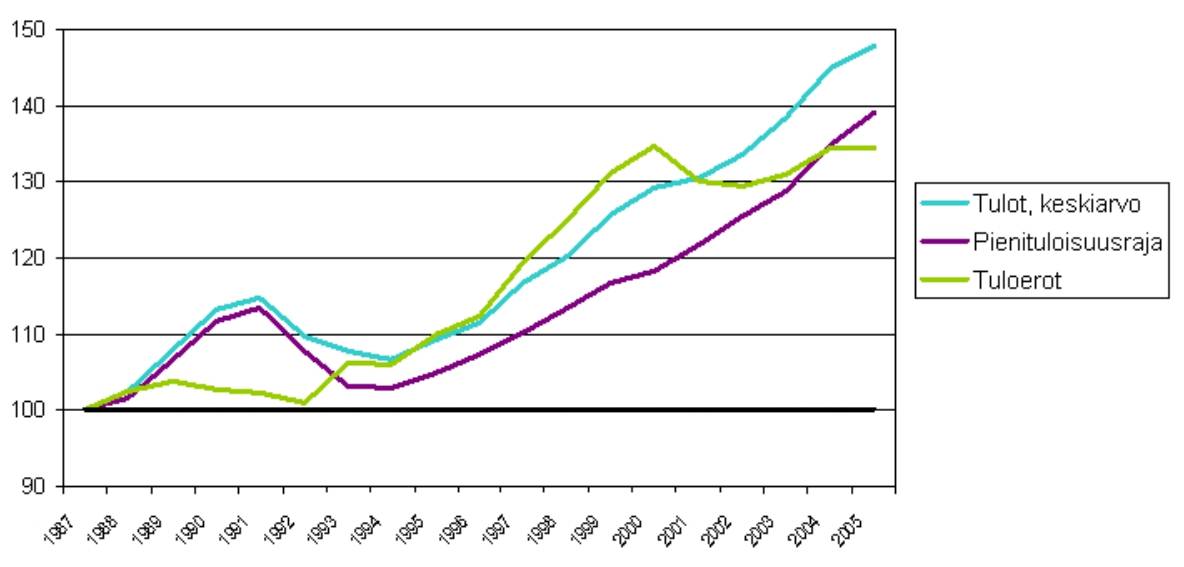
\includegraphics[width=1\linewidth]{images/tuloerot} 

}

\caption{Tuloerot.}\label{fig:tuloerot}
\end{figure}

\hypertarget{alaluku53}{%
\section{Mittaaminen ja mitta-asteikot}\label{alaluku53}}

\textbf{Mittaaminen}

\begin{itemize}
\tightlist
\item
  Kumpaa tahansa tutkimusotetta (kokonais- tai otantatutkimus) noudatettaessa tietojen keräämisessä on olennaisena osana kohteiden ominaisuuksien \textbf{mittaaminen}.
\item
  Tilastotieteellinen tutkimus perustuu aina mitattaviin satunnaisilmiöihin: tavoitteena on mittaamalla liittää jokin luku ilmiötä kuvaavaan ominaisuuteen, ts. mitata kyseisen satunnaismuuttujan havaittua arvoa.

  \begin{itemize}
  \tightlist
  \item
    Mittaaminen vaatii aina mittauksen kohteen, hyvin määritellyn mitattavan ominaisuuden ja \textbf{mittarin}, joka liittää mielekkäät lukuarvot mitattavaan ominaisuuteen.
  \item
    Erilaiset mittarit heijastavat ilmiön ominaisuuksia eri tavoin ja eri tarkkuudella

    \begin{itemize}
    \tightlist
    \item
      Esimerkiksi, jos tutkitaan opiskelijoiden pituuden kehitystä, niin mitataan pituutta eri aikoina. Pituudet voidaan mitata senttimetreissä, metreissä, kilometreissä tai vaikkapa tuumissa.
    \item
      Mittari on hyvä, jos sen antama mittaus on

      \begin{itemize}
      \tightlist
      \item
        \textbf{(i) validi} eli mittaus esittää oikein mitattavaa ominaisuutta (senttimetri mittaa pituutta, gramma ei) ja
      \item
        \textbf{(ii) luotettava} eli mittaus on \textbf{harhaton} ja \textbf{toistettavissa}.
      \end{itemize}
    \item
      Määritellään nämä termit vielä erikseen, sillä ne ovat keskeisiä tilastotieteessä.
    \end{itemize}
  \end{itemize}
\end{itemize}

\begin{defblock}{}
\textbf{Harhattomuus}

Mittari on harhaton, jos se ei systemaattisesti ali- tai yliarvioi mitattavan ominaisuuden määrää.

\end{defblock}

\begin{itemize}
\item
  Harhaton mittari siis antaa keskimäärin oikeita mittauksia mitattavasta ominaisuudesta.
\item
  Harhattomuutta pidetään myös hyvänä ominaisuutena tilastollisten mallien parametrien estimaattoreille. Tähän palataan myöhemmin luvussa \ref{luku6}.
\end{itemize}

\begin{defblock}{}
\textbf{Toistettavuus}

Mittari on toistettava, jos se tuottaa keskimäärin samanlaisia mittauksia samanlaisista otoksista eli se on johdonmukainen ja mittausvirheet ovat pieniä.

\end{defblock}

\begin{itemize}
\item
  Huonosti toistettava mittari antaa tilastoyksiköiden samankaltaisille ominaisuuksille hyvin erilaisia arvoja riippuen otoksesta.
\item
  \textbf{Mittausten reliabiliteettia/luotettavuutta} arvioidessa voidaan pohtia esimerkiksi seuraavia kysymyksiä:

  \begin{itemize}
  \tightlist
  \item
    Kuinka hyvin mittaustulokset ovat toistettavissa? Kuinka paljon niissä on ei-sattumanvaraisuutta?
  \item
    Mittausten validiteetti: kuinka hyvin pystyttiin mittaamaan sitä, mitä oli tarkoitus mitata?
  \end{itemize}
\item
  Kun mittaaminen on luotettavaa ja validia, tutkimusaineisto on \textbf{sisäisesti luotettavaa}.
\item
  Aineiston \textbf{ulkoinen luotettavuus} toteutuu silloin, kun tutkittu otos edustaa perusjoukkoa eli on edustava.

  \begin{itemize}
  \tightlist
  \item
    Validi mittaaminen ei pelasta otosta, jos se ei ole edustava!
  \end{itemize}
\item
  Jokaisen tutkimuksen tulosten luotettavuuden perusteena on käytetty aineisto, kuinka se on hankittu ja mistä lähteestä. Kun käytetään luotettavaksi havaittuja mittareita, voidaan kustakin aineistosta laskea erikseen tunnuslukuja mittauksen luotettavuudelle. Esimerkkinä \textbf{luottamusväli}:

  \begin{itemize}
  \tightlist
  \item
    Väli, joka vaihtelee otoksesta toiseen ja joka usein sisältää mielenkiinnon kohteena olevan parametrin, kun otantakoetta toistetaan!
  \item
    Luottamusväliä käytetään määrittämään estimaatin luotettavuutta.
  \item
    Väliestimointia tarkastellaan tarkemmin luvussa \ref{luku6}.
  \end{itemize}
\end{itemize}

\begin{figure}

{\centering 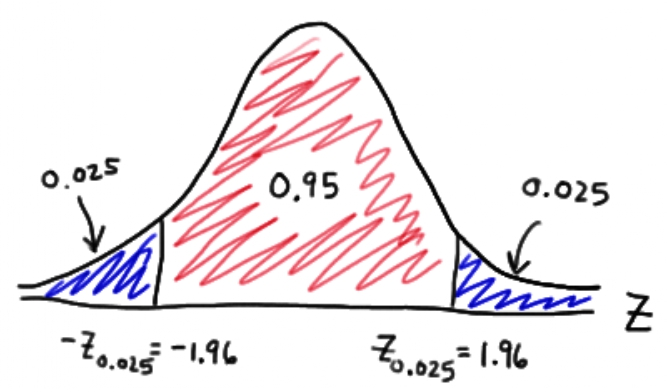
\includegraphics[width=0.75\linewidth]{images/luottamus} 

}

\caption{Normaalijakaumaan perustuva 95\% luottamusväli.}\label{fig:luottamus}
\end{figure}

\begin{itemize}
\tightlist
\item
  Luotettavuudella voidaan tarkoittaa myös tutkimuksen \textbf{objektiivisuutta / puolueettomuutta}

  \begin{itemize}
  \tightlist
  \item
    \textbf{Objektiivinen totuus}, tutkimustulokset ovat samat riippumatta siitä kuka pätevä tutkija tutkimuksen on tehnyt.
  \item
    Tulosten tulisi olla luotettavia, mutta luotettavatkin tulokset voivat olla puolueellisia siinä mielessä, että ne tarkastelevat asiaa vain yhdeltä näkökannalta!
  \item
    Esim. tarkastellaan yrityksen henkilöstökysymyksiä, työn organisointia ja työmoraalia, ongelmien tarkastelua johdon vs.~henkilöstön näkökulmasta.
  \end{itemize}
\end{itemize}

\begin{eblock}{}

\textbf{Esimerkki: C-vitamiinin vaikutus syövän hoidossa}

\begin{itemize}
\tightlist
\item
  Annettiin C-vitamiinia 100:lle terminaalivaiheen syöpäpotilaalle ja
  seurattiin kuolleisuutta (Cameron and Pauling, 1976).

  \begin{itemize}
  \tightlist
  \item
    Pyrittiin luomaan tärkeiden ominaisuuksien suhteen samanlaisia verrokkiryhmiä ja valittiin kutakin potilasta kohden 10 verrokkia, jotka olivat samanlaisia iän, sukupuolen, primääri-kasvaimen sijaintipaikan ja histologisen kasvaintyypin suhteen.
  \item
    Seuranta-aika: aika hetkestä, jolloin todettiin tavanomaisten hoitojen olevan tehottomia, kuolinhetkeen saakka.
  \item
    Tulos: C-vitamiinia saaneet käsittelyryhmän potilaat elivät 4 kertaa kauemmin (p \(< 0.0001\)).
  \end{itemize}
\item
  Ristiriitaista evidenssiä saatiin tutkimuksessa, jossa vastaava tutkimusongelma, mutta toteutettu satunnaistettuna kokeena (Moertel et al.~1985).

  \begin{itemize}
  \tightlist
  \item
    Satunnaistettiin potilaat, joilla pitkälle edennyt paksunsuolen tai peräsuolen syöpä, C-vitamiinia saavien ja lumelääkettä saavien ryhmiin.
  \item
    Tulos: kontrolliryhmän potilaat elivät keskimäärin hieman pidempään, mutta ero ei tilastollisesti merkitsevä.
  \end{itemize}
\item
  Mistä kahden tutkimuksen erot johtuivat?

  \begin{itemize}
  \tightlist
  \item
    Huonolla tuurilla kaltaistetut verrokit erosivat käsittelyryhmän potilaista joillakin merkittävillä tavoilla, joita ei oltu mitattu! Miten kvantifioida ``huonoa tuuria''?
  \end{itemize}
\item
  Tilastolliset menetelmät tekevät juuri tämän: ``Mikä on todennäköisyys, että havaittu tulos (tai sitä enemmän nollahypoteesista poikkeava tulos) olisi syntynyt vain sattumalta?''

  \begin{itemize}
  \tightlist
  \item
    Ilman satunnaistamista tuota kenties merkittävää ei-mitattua eroa ei pystytä varmuudella kontrolloimaan.
  \item
    Todellisuudessa ero johtui siitä, että ensin mainitun tutkimuksen kontrollit valittiin jo kuolleista syöpäpotilaista, eikä heihin liittynyt enää mitään satunnaisuutta!
  \end{itemize}
\end{itemize}

\end{eblock}

\hfill\break

\textbf{Mitta-asteikot}

\begin{itemize}
\item
  Kuten satunnaismuuttujia koskeneessa luvussa \ref{luku4} opittiin, satunnaisilmiöillä on erilaisia tulosvaihtoehtoja, jotka kantavat satunnaismuuttujien todennäköisyysjakaumia.

  \begin{itemize}
  \tightlist
  \item
    On syytä huomauttaa, että vaikka mitattava ilmiö ei olisikaan numeerinen, se voidaan aina ``koodata'' eli muuntaa numeeriseksi. Esimerkiksi perinteinen kaksiarvoinen mies-nainen -muuttujan tapauksessa voidaan käyttää tunnuksia 0 ja 1.
  \end{itemize}
\item
  Ilmiön luonteesta riippuen voidaan näille tulosvaihtoehdoille käyttää erilaisia \textbf{mitta-asteikkoja}.

  \begin{itemize}
  \tightlist
  \item
    \textbf{Laatueroasteikko/luokitteluasteikko} (nominaaliasteikko): Muuttujan mittaustaso on tällöin sellainen, että sen arvot voidaan luokittaa toisistaan eroaviin luokkiin. Ts. mihin luokkaan kohde kuuluu mitattavan ominaisuuden perusteella?

    \begin{itemize}
    \tightlist
    \item
      Tilastoyksiköt luokitellaan ennaltamääriteltyihin luokkiin. Luokkien järjestyksellä ei ole merkitystä.
    \item
      Kukin tilastoyksikkö kuuluu vain yhteen luokkaan. Tällöin kahdesta tilastoyksiköstä/havainnosta voidaan päätellä vain kuuluvatko ne saamaan luokkaan vai eivät.
    \item
      Emme pysty määrittelemään empiirisesti mielekästä järjestystä havaintoarvojen välillä.
    \item
      Esimerkkejä: Sukupuoli, veriryhmä tai kotikunta.
    \end{itemize}
  \item
    \textbf{Järjestysasteikko} (ordinaaliasteikko): Tällöin muuttujan arvot voidaan luokittelun lisäksi asettaa empiirisesti mielekkääseen järjestykseen. Tällöin siis mittauksen kohteella on ``enemmän mitattavaa ominaisuutta'' kuin jollakin toisella kohteella

    \begin{itemize}
    \tightlist
    \item
      Tilastoyksiköt luokitellaan ennalta määrättyihin luokkiin, joilla on yksikäsitteinen järjestys.
    \item
      Esimerkkejä: Sotilasarvo, sosiaaliryhmä, kilpailun tulos tai sairauksien tarttuvuus.
    \end{itemize}
  \item
    \textbf{Välimatka-asteikko} (intervalliasteikko): Luokittamisen ja järjestyksen asettamisen lisäksi havaintoarvojen välimatkalla on empiirisesti mielekäs tulkinta. Ts. intervalliasteikon tasoisen muuttujan arvoista voidaan sanoa, kuinka paljon toinen arvo on toista suurempi (pienempi).

    \begin{itemize}
    \tightlist
    \item
      Välimatka-asteikolla pystytään mittaamaan yksittäisten luokkien tai havaintoarvojen ero. Esimerkiksi: Lämpötilan mittaaminen esim. celcius-asteina. Pystymme numeroarvoina ilmoittamaan onko tänään lämpimämpi, yhtä lämmin vai kylmempi sää kuin eilen ja kuinka monta astetta muutos on.
    \item
      Kuinka paljon kahden mittauksen kohteen ominaisuudet eroavat toisistaan.
    \item
      Intervalliasteikon tasoisen muuttujan arvoista voidaan sanoa, kuinka paljon toinen arvo on toista suurempi (pienempi). Mittarin nollapiste on kuitenkin ``keinotekoinen'' ja siten vapaasti valittavissa. Samoin voidaan valita käytettävä mittayksikkö vapaasti. Oleellista on vain se, että havaintojen välisellä välimatkalla on aina empiirisesti mielekäs tulkinta.
    \item
      Yhteen- ja vähennyslasku ovat sallittuja.
    \end{itemize}
  \item
    \textbf{Suhdeasteikko}: Jos intervalliasteikon ominaisuuksien lisäksi on määriteltynä yksikäsitteinen mittalukujen absoluuttinen nollapiste.

    \begin{itemize}
    \tightlist
    \item
      Esimerkiksi kuuden euron hintainen tuote on kaksi kertaa niin kallis kuin kolmen euron tuote.
    \item
      Kunnan veroäyri tai henkilön pituus: Absoluuttinen nollapiste on 0.
    \item
      Nollapisteen ollessa absoluuttinen, se ``pysyy paikallaan'' ja mittalukujen suhteet pysyvät samoina.
    \end{itemize}
  \end{itemize}
\item
  Mitta-asteikot voidaan jakaa kahteen luokkaan: \textbf{Luokittelu- ja järjestysasteikkoa kutsutaan kvalitatiivisiksi asteikoiksi}. Tällöin muuttujien arvot kuvaavat vain tilastoyksiköiden laadullisia piirteitä.
\item
  Vastavasti \textbf{välimatka- ja suhdeasteikkoa kutsutaan kvantitatiivisiksi asteikoiksi}, koska tällöin mittaluvut kuvaavat jonkin ominaisuuden määrää.
\item
  Tilastollisen analyysin kannalta mitta-asteikkojen merkitys on siinä, että tilastollisten (matemaattisten) operaatioiden sallittavuus määräytyy muuttujan mitta-asteikon mukaan. Mitä ``korkeampi'' mitta-asteikko, sitä enemmän on käytettävissä olevia analyysimenetelmiä. Esimerkiksi keskiarvon laskeminen on eräs tilastollinen operaatio, ja se ei ole sallittu kvalitatiivislle muuttujille.
\end{itemize}

\hfill\break
\textbf{Aineistotyyppejä}

\begin{itemize}
\tightlist
\item
  Käsitellään tarkemmin vielä myöhemmin (Luvussa \ref{luku10}), joiden yhteydessä mitattavat muuttujat voivat olla kvalitatiivisia tai kvantitatiivisia.

  \begin{itemize}
  \tightlist
  \item
    Poikkileikkausaineisto: Tietoja useista tutkimuskohteista yhdeltä ajanhetkeltä tai aikäväliltä
  \item
    Aikasarja-aineisto: Tietoja samasta tutkimuskohteesta eri ajanhetkiltä
  \item
    Paneeliaineisto: Tietoja useilta ajanhetkiltä useista tutkimuskohteista
  \item
    Tapahtumahistoria-aineisto: Tietoja tapahtumahetkiltä
  \end{itemize}
\end{itemize}

\hypertarget{alaluku54}{%
\section{Kontrolloidut kokeet ja suorat havainnot}\label{alaluku54}}

\begin{itemize}
\item
  Tilastollinen tutkimusaineisto voidaan kerätä:

  \begin{itemize}
  \tightlist
  \item
    \textbf{Kontrolloiduilla kokeilla}, joissa tutkimuksen kohteet altistetaan suunnitelmallisesti erilaisiin koeolosuhteisiin selvittääkseen miten kohteet reagoivat muutoksiin.
  \item
    \textbf{Suoria havaintoja} tehtäessä koeolosuhteita ei pyritä aktiivisesti muuttamaan vaan ainoastaan seurataan miten erilaiset olosuhteet ja niissä tapahtuvat muutokset vaikuttavat kohteisiin.
  \end{itemize}
\item
  Näistä tutkimusasetelmista kontrolloidut kokeet ovat tietenkin ihanteellisempia tutkimuksen tekemiselle, sillä tutkijan on mahdollista tarkastella tutkittavaa asiaa koeolosuhteissa ``eristyksissä''.
\item
  Kontrolloidut kokeet eivät kuitenkaan ole aina mahdollisia, jolloin on käytettävä suoria havaintoja.

  \begin{itemize}
  \tightlist
  \item
    Tällöin tutkimuskohdetta ei suunnitelmallisesti altisteta koeolosuhteille (``käsittelyille'') vaan muuttuvien olosuhteiden vaikutuksia tilastoyksikköihin seurataan passiivisesti.
  \item
    Toisin sanoen tutkimuksen kohteena olevat tilastoyksiksöt eivät välttämättä edes tiedä osallistuvansa tutkimukseen.
  \end{itemize}
\item
  Lisäksi usein tehdään hoito/käsittelyvastetta koskevia vertailuja erilaisissa olosuhteissa, joka osaltaan vaikuttaa tulosten uskottavuuteen, sillä tutkittaviin tilastoyksiköihin voi vaikuttaa olosuhteiden muutosten lisäksi muut ulkopuoliset tekijät.

  \begin{itemize}
  \tightlist
  \item
    Näiden \textbf{selittävien} ja \textbf{sekoittavien tekijöiden} vaikutusten kontrollointi on suoria havaintoja tehtäessä vaativa tehtävä.
  \item
    Mikäli ulkopuolisia tekijöitä ei havaita ja/tai pystytä mittaamaan, tai muuten jostain syystä olla lisätty ja käytetty käytettävässä tilastollisessa mallissa, voi kyseeseen tulla ns. \textbf{puuttuvien selittäjien harha}, joka tarkoittaa sitä että havaittuihin tuloksiin vaikuttaa jokin havaitsematon tekijä, jonka vaikutusta ei kyetä kvantifioimaan puutteellisten havaintoarvojen vuoksi.
  \end{itemize}
\item
  Suoria havaintoja tehtäessä ei voida (usein) selvittää vasteen ja olosuhteiden \textbf{kausaalista} yhteyttä. Suorilla havainnoilla voidaan lähinnä saada selville onko vasteella ja olosuhteilla jokin yhteys (korrelaatio) (ks. luku \ref{luku7}).
\item
  Suorien havaintojen keräämiseen liittyy olennaisesti joitain riskejä ja toisaalta rajoituksia. Riskit liittyvät käytännössä otoksen harhaisuuteen (erit. valikoitumisharha).

  \begin{itemize}
  \tightlist
  \item
    Esimerkiksi jos havaintoja tehtäessä suositaan systemaattisesti joitakin tulosvaihtoehtoja. Tämä suosiminen voi olla tahallista tai tahatonta.
  \item
    Tämä tilastoyksiköiden \textbf{valikoituminen} otokseen aiheuttaa harhaa, sillä otokseen valikoituva osajoukko saattaa ylikorostaa perusjoukon joitain ominaisuuksia.
  \end{itemize}
\end{itemize}

\begin{defblock}{}

\textbf{Valikoituminen}

Valikoitumista tapahtuu, jos otokseen poiminta ei ole riippumatonta tilastoyksikön ominaisuuksista. Tätä kutsutaan valikoitumisharhaksi.

\begin{itemize}
\item
  Esimerkiksi verrattaessa sydän- ja verisuonitautipotilaiden hoitotoimenpiteitä potilaat eivät mahdollisesti ole valikoituneet yhtä todennäköisesti pallolaajennukseen, ohitusleikkaukseen tai lääkehoitoryhmään, sillä taudin vakavuus saattaa jo määritellä mikä hoitotoimenpide valitaan.
\item
  Valikoituminen on iso ongelma seurantatutkimuksissa, sillä harhaisten havaintotulosten, eli harhaisen otoksen, perusteella ei voida tehdä luotettavia johtopäätöksiä perusjoukosta!
\end{itemize}

\end{defblock}

\begin{itemize}
\tightlist
\item
  Harhan syntymistä pyritään välttämään valitsemalla havaintojen kohteet perusjoukosta satunnaisesti (ellei tavoitteena ole tutkia kaikkia perusjoukon alkioita). Tämä merkitsee satunnaisotannan soveltamista havaintojen kohteiden valintaan, eli otokseen poimittavien tilastoyksiköiden valintaan sovelletaan \textbf{satunnaistamista}, jolloin sattuma määrää mitkä perusjoukon alkioista tulevat poimituksi otokseen (tutkimuksen kohteiksi)!
\end{itemize}

\begin{defblock}{}

\textbf{Satunnaistaminen}

Tilastoyksiköiden poimimista populaatiosta otokseen riippumatta muiden yksiköiden poiminnasta tai kyseisten (poimittavien) yksiköiden ominaisuuksista.

\begin{itemize}
\item
  Satunnaistaminen takaa sen, että mahdolliset sekoittavat tekijät ovat jakaantuneet tasaisesti tutkittavassa joukossa. Tällöin sekoittavat tekijät eivät aiheuta harhaa otokseen ja tutkimuksen tulokset voidaan yleistää koko populaatioon.
\item
  Satunnaistaminen poistaa otannasta valikoitumisharhan, sillä otokseen poiminta suoritetaan riippumatta tilastoyksiköiden ominaisuuksista. Satunnaistaminen on ainoa puolueeton tapa poimia otos (ei suosi mitään perusjoukon osaa)!
\end{itemize}

\end{defblock}

\begin{itemize}
\item
  Satunnaistaminen (osaltaan) mahdollistaa \textbf{tilastollisen päättelyn}, jonka avulla otoksesta saatuja tietoja voidaan hyödyntää tehtäessä päätelmiä koko perusjoukosta.

  \begin{itemize}
  \tightlist
  \item
    Tilastollisen päättelyn avulla voidaan muodostaa esimerkiksi jakaumien ja tilastollisten mallien tuntemattomille parametreille arviot (piste-estimaatit) ja arvioida niiden epävarmuutta (keskivirheet ja luottamusvälit) sekä testata tarkasteltavaan ilmiöön liittyviä hypoteeseja (ks. luku \ref{luku6}).
  \end{itemize}
\item
  Johtopäätelmien pätevyys riippuu mm. siitä, kuinka hyvin otanta on suoritettu. Tämän vuoksi on tärkeää ymmärtää otannan perusperiaatteet ja erilaisten otantamenetelmien luonne.
\item
  Kontrolloiduissa kokeissa satunnaistaminen jakaa yksilöt \textbf{riippumatta yksilön omista ilmiöön vaikuttavista muuttujista} joko \textbf{käsittely- tai kontrolliryhmään} (eng. treatment ja control).

  \begin{itemize}
  \tightlist
  \item
    Se takaa, ettei valikoitumista jonkin käsittelyä edeltävän ominaisuuden mukaan esiinny.
  \item
    Tämä tarkoittaa \textbf{altisteen} (käsittely / ``treatment'') antamista (täysin) satunnaisesti kokeeseen valituille yksilöille, riippumatta näiden taustamuuttujien arvoista.
  \item
    Nämä yksilöt sinänsä voivat olla satunnaisotos jostain populaatiosta (tai ainakin niiden toivotaan olevan), mutta satunnaistaminen tarkoittaa siis käsittelyn kohdentamista koeyksilöille, ei satunnaisotantaa sinänsä.
  \item
    Esimerkiksi tutkittavat voidaan satunnaistaa lääkehoito- ja placeboryhmiin, jotta mahdolliset erot tutkittavien iässä, sukupuolessa ja muissa taustamuuttujissa eivät aiheuta systemaattista harhaa, kun tutkitaan lääkehoidon vaikutusta.
  \end{itemize}
\end{itemize}

\hypertarget{alaluku55}{%
\section{Otantamenetelmät}\label{alaluku55}}

\begin{itemize}
\tightlist
\item
  Tässä jaksossa tarkastellaan erilaisia \textbf{otantamenetelmiä}. Näiden menetelmien tarkoitus on suorittaa otosaineiston (tutkimusaineiston) kerääminen niin, että se huomioi aiemmin esitellyt hyvän otannan kriteerit, ts. että sen tuottama otos on edustava ja luotettava. Näin ollen otos kuvaa koko perusjoukkoa.

  \begin{itemize}
  \tightlist
  \item
    Otantamenetelmän, joskus myös \textbf{otanta-asetelman}, valinta on tietenkin vahvasti sovellusalakohtainen: käytettävät aineistot ja täten otantamenetelmät määräytyvät pitkälti tehtävän tutkimuksen luonteen perusteella. Ts. käytännön tilanteet poikkeavat toisistaan lopulta varsin paljon ja eri tilanteisiin tarvitaan omat menetelmänsä.
  \item
    Otanta-asetelmalla tarkoitetaan erityisesti otoksen poimintaan käytettyä \textbf{satunnaistuksen menetelmää}.
  \end{itemize}
\item
  Otannan tavoitteena on tietenkin \textbf{edustava otos}. Otoksen edustavuuteen vaikuttaa käytännön otannassa se, miten todennäköistä kullakin perusjoukon alkiolla (populaation tilastoyksiköllä) on tulla poimituksi otokseen. Tätä kutsutaan \textbf{sisältymistodennäköisyydeksi}.
\end{itemize}

\begin{defblock}{}
\textbf{Sisältymistodennäköisyys}

Sisältymistodennäköisyys kuvaa sitä (tunnettua) todennäköisyyttä, jolla perusjoukon alkio tulee poimituksi otokseen.

\end{defblock}

\begin{itemize}
\tightlist
\item
  Käytännössä otoksen poiminta suoritetaan niin, että \(n\):n alkion otos (\(n\) on otoskoko) poimitaan jollakin satunnaisotannan menetelmällä \(N\):n alkion perusjoukosta (\(N\) on siis perusjoukon koko).
\item
  Perusjoukon yksittäinen alkio (tilastoyksikkö) \(k\) tulee poimituksi \(n\):n alkion otokseen (tutkimusaineistoon) tunnetulla \textbf{sisältymistodennäköisyydellä} \(\pi_k\),
  \[
  0 < \pi_k \le 1, \quad k = 1, \ldots, N,
  \]
  jossa siis \(N\) on perusjoukon alkioiden lukumäärä. Toisin sanoen, kaikilla perusjoukon alkioilla on oma nollaa suurempi todennäköisyytensä (voi olla 1), \(\pi_k\), tulla poimituksi otokseen.

  \begin{itemize}
  \tightlist
  \item
    Sisältymistodennäköisyys voi olla sama kaikille perusjoukon alkioille tai vaihdella perusjoukon eri osajoukkojen (alkioryhmien) välillä. Tämä tulee huomioida otantamenetelmän valinnassa, jotta saadun otoksen edustavuus ei vaarannu.
  \item
    Sisältymistodennäköisyyttä voidaan käyttää monimutkaisemmassa otantateoriassa \textbf{asetelma}- ja \textbf{analyysipainojen} muodostamisessa sekä uudelleenpainotuksessa (vastauskadon korjaus).
  \end{itemize}
\item
  Tässä luvussa käsitellään erilaisia perinteisiä otantamenetelmiä sekä sitä, minkälaisten perusjoukkojen tilanteissa mikäkin otantamenetelmä on sopivin.

  \begin{itemize}
  \tightlist
  \item
    \textbf{Yksinkertainen satunnaisotanta} (YSO): perinteisin otantamenetelmä, jossa jokaisella tietyn kokoisella otoksella sama mahdollisuus tulla valituksi.
  \item
    \textbf{Systemaattinen otanta} (SYS): eli tasavälisessä, otannassa poimintakehikkoon (perusjoukkoon) kuuluvat alkiot järjestetään jonoon ja siitä poimitaan otokseen joka k. alkio.
  \item
    \textbf{Ositettu otanta}: perusjoukko (populaatio) jaetaan ominaisuuksiltaan yhtenäisiin eli homogeenisiin \textbf{ositteisiin}, joista jokaisesta poimitaan erillinen otos.
  \item
    \textbf{Ryväsotanta} tai joskus myös \textbf{moniasteinen otanta}: Hyödynnetään perusjoukossa esiintyvää kerroksellisuutta, eli hierarkkisuutta otannassa.
  \end{itemize}
\end{itemize}

\hypertarget{yksinkertainen-satunnaisotanta}{%
\subsection{Yksinkertainen satunnaisotanta}\label{yksinkertainen-satunnaisotanta}}

\begin{itemize}
\tightlist
\item
  \textbf{Yksinkertaisessa satunnaisotannassa} (YSO) jokaisella tilastoyksiköllä (perusjoukon alkiolla) on nollasta poikkeava todennäköisyys tulla valituksi otokseen.

  \begin{itemize}
  \tightlist
  \item
    Otannan satunnaisuus tulee siis siitä, että jokainen tilastoyksikkö poimitaan otokseen \emph{satunnaisesti}! (Ks. luku \ref{luku4})
  \item
    YSOaa pidetään otannan perusmuotona, jossa jokaisella perusjoukon alkiolla on lähtökohtaisesti yhtä suuri todennäköisyys tulla valituksi otokseen.

    \begin{itemize}
    \tightlist
    \item
      YSO on periaatteiltaan intuitiivinen ja helppo ymmärtää. Lisäksi se on tietyissä tilanteissa usein helppo toteuttaa.
    \end{itemize}
  \item
    Tällöin on selvää että myös jokaisella perusjoukon samankokoisella osajoukolla on sama todennäköisyys tulla valituksi.
  \item
    Toisin sanoen, todennäköisyys tulla poimituksi ei riipu tilastoyksikön ominaisuuksista tai siitä minkälaisia ominaisuuksia jo poimituilla otosyksiköillä on.
  \item
    Satunnaisotanta siis selvästi korjaa valikoitumisharhaa (ks. aiempi luku \ref{alaluku54}) satunnaistamalla otokseen valikoitumisen täysin! YSO voidaankin aina tulkita arvonnaksi. Käytännön työssä arvonta onkin oiva satunnaistamisen keino.
  \end{itemize}
\item
  \textbf{YSO:n toteuttaminen}

  \begin{itemize}
  \tightlist
  \item
    Käytännössä yksinkertainen satunnaisotanta etenee vaiheittain:

    \begin{itemize}
    \tightlist
    \item
      Tutkimuksen alussa tutkijalla tulisi olla käytettävänään (ts. tulisi koostaa) lista kaikista perusjoukon havaintoyksiköistä \textbf{(alkioista)}. Tämä muodostaa tutkimuksen \textbf{otantakehikon}.
    \item
      Tämän jälkeen jokaiseen perusjoukon alkioon voidaan liittää numeeriset tunnukset.
    \item
      Sitten valitaan haluttu otoksen koko. Otoskoon määrittäminen on keskeinen osa koesuunnittelua, ks. luku \ref{alaluku66}
    \item
      Otantakehikosta arvotaan perusjoukon alkiot otokseen yksi kerrallaan.
    \item
      Käytännössä arvonta voidaan toteuttaa satunnaislukuja generoimalla (tuottamalla) niin että jokaisen otantakehikon alkion sisältymistodennäköisyys on yhtä suuri.\footnote{Satunnaislukujen generointia käsitellään ja opetellaan mm. kursseilla \href{https://opas.peppi.utu.fi/fi/opintojakso/TILM3517/5068?period=2022-2024}{TILM3517 R-kielen alkeet} ja \href{https://opas.peppi.utu.fi/fi/opintojakso/TILM3705/92210}{TILM3705 Johdatus laskennalliseen tilastotieteeseen.}}
    \end{itemize}
  \end{itemize}
\item
  YSO:n \textbf{poimintastrategiat}: Käytännössä yksinkertainen satunnaisotanta voidaan suorittaa kahdella eri tavalla: \textbf{palauttaen} tai \textbf{palauttamatta}.

  \begin{itemize}
  \tightlist
  \item
    Tarkastellaan, aiemman mukaisesti, \textbf{äärellistä populaatiota} (perusjoukkoa), jossa on \(N\) alkiota ja tarkoituksena on poimia \(n\):n alkion kokoinen otos (huom. \(n<N\)). Olkoon \(i\) yksittäisen alkion indeksiluku (ts. jokainen alkio on numeroitu esimerkiksi tavalla \(i = 1,\ldots,N\)).
  \end{itemize}
\end{itemize}

\textbf{YSO:n poiminta palauttaen}

\begin{itemize}
\tightlist
\item
  Kun poiminta suoritetaan \textbf{palauttaen}, niin poimittu alkio palautetaan aina ennen uuden alkion arpomista takaisin perusjoukkoon, jolloin alkio voi tulla poimituksi otokseen useita kertoja.

  \begin{itemize}
  \tightlist
  \item
    Kyseessä on siis otanta \textbf{takaisinpanolla} (with replacement).
  \item
    Tällöin alkioiden arvonnat ovat riippumattomia: alkion todennäköisyys tulla poimituksi otokseen ei riipu siitä kuinka monta alkiota otokseen on jo poimittu.
  \item
    Alkion \(i\) sisältymistodennäköisyys on tällöin selvästi
  \end{itemize}
\end{itemize}

\[
\pi_i = \frac{1}{N}, \quad \forall \, i
\]

\begin{itemize}
\item
  Otantaan palauttaen liittyviä todennäköisyyksiä hallitaan \textbf{binomijakauman} avulla (ks. luku \ref{luku4}), joka johtaa yksinkertaiseen \textbf{tilastolliseen malliin} YSO:a käytettäessä.
\item
  Poiminta palauttaen, tai otanta takaisinpanolla, on toisaalta varsin epärealistinen otantamenetelmä useassa tutkimuksessa. Esimerkiksi lienee mahdotonta testata samaa lääkettä useaan otteeseen samaan aikaan yhdellä koehenkilöllä.
\end{itemize}

\textbf{YSO:n poiminta palauttamatta}

\begin{itemize}
\tightlist
\item
  Kun poiminta suoritetaan \textbf{palauttamatta}, poimittua alkiota ei palauteta perusjoukkoon poiminnan jälkeen eikä se täten voi tulla poimituksi otokseen kuin kerran.

  \begin{itemize}
  \tightlist
  \item
    Kyseessä on siis otanta \textbf{ilman takaisinpanoa} (without replacement).
  \item
    Tällöin alkioiden arvonnat eivät enää ole riipumattomia: alkion todennäköisyys tulla poimituksi otokseen riippuu siitä kuinka monta alkiota otokseen on jo poimittu.
  \item
    Alkion \(i\) sisältymistodennäköisyys on tällöin vastaavasti
  \end{itemize}
\end{itemize}

\[
\pi_i = \frac{1}{N - A_i},
\]

\begin{itemize}
\tightlist
\item
  Tässä \(A_i\) on jo poimittujen alkioiden lukumäärä ennen kyseistä \textbf{otositeraatiota}: ensimmäisen poiminnan kohdalla \(A_i = 0\), toisen kohdalla \(A_i = 1\) ja niin edespäin.

  \begin{itemize}
  \tightlist
  \item
    Ilman takaisinpanoa populaatiosta voidaan poimia \({N \choose n}\) erilaista otosta.\footnote{Kun otosyksiköiden järjestyksellä ei ole merkitystä. \({N \choose n}\) on ns. binomikerroin, joka saadaan kaavasta \({N \choose n} = \frac{N!}{n!(N-n)!},\) jossa \(N! = N \cdot (N-1) \cdot (N-2) \cdots 1\) on \(N\):n kertoma.}
  \item
    Otantaan palauttamatta liittyviä todennäköisyyksiä hallitaan \textbf{hypergeometrisen jakauman} avulla, joka johtaa (melko) yksinkertaiseen \textbf{tilastolliseen malliin} YSO:a käytettäessä.
  \end{itemize}
\end{itemize}

\newpage

\begin{eblock}{}

\textbf{Esimerkki: Yksinkertaisen satunnaisotannan poimintastrategiat}

\begin{itemize}
\tightlist
\item
  Esimerkki: Poimitaan palloja kulhosta satunnaisesti.

  \begin{itemize}
  \tightlist
  \item
    Jos yksittäinen pallo (alkio) voi tulla poimituksi useammin kuin kerran, eli pallo palautetaan kulhoon sen poiminnan jälkeen, on kyseessä yksinkertainen satunnaisotanta takaisinpanolla.
  \item
    Vastaavasti jos pallo voi tulla valituksi vain kerran, eli pallo poistetaan kulhosta sen poiminnan jälkeen, on kyseessä otanta ilman takaisinpanoa.
  \end{itemize}
\end{itemize}

\end{eblock}

\textbf{Otoskoon vaikutus YSO:n}

\begin{itemize}
\tightlist
\item
  Yksinkertaisen satunnaisotannan erot takaisinpanolla ja ilman takaisinpanoa riippuvat otantakehikon (tai yleisemmin perusjoukon) koosta. Mikäli poimittava otos muodostaa suuren osan perusjoukosta (ts. \(\frac{n}{N}\) on ``suuri'', eli lähellä yhtä) menetelmät poikkeavat olennaisesti.
\item
  Toisaalta, jos perusjoukko on ääretön niin menetelmillä ei ole käytännössä eroa (ts. kun \(N \longrightarrow \infty\) niin \(\frac{n}{N} \longrightarrow 0\) eli todennäköisyys että sama alkio poimittaisiin otokseen useammin kuin kerran lähestyy nollaa otoskoon lähestyessä ääretöntä).

  \begin{itemize}
  \tightlist
  \item
    Monesti onkin (teoreettiselta) kannalta järkevää olettaa että otos poimitaan äärettömästä perusjoukosta vaikka perusjoukko tosiasiallisesti olisikin äärellinen (mutta riittävän ``iso'').
  \item
    Tällöin voidaan olettaa käytettävän otantaa takaisinpanolla, sillä siinä käytettävät tilastolliset mallit ovat yksinkertaisempia kuin otannassa ilman takaisinpanoa ja tämä helpottaa tilastollisessa päättelyssä käytettäviä kaavoja.
  \end{itemize}
\end{itemize}

\textbf{YSO: Potentiaaliset ongelmat}

\begin{itemize}
\tightlist
\item
  Monissa tapauksissa ei kuitenkaan ole helppoa saada listaa kaikista perusjoukon havaintoyksiköistä (jolloin menetelmän käyttö on mahdotonta).
\item
  Kyselytutkimuksissa perusjoukko on usein suuri ja laajalle alueelle hajaantunut. Henkilökohtaisten, kasvotusten toteutettavien, haastattelujen tekeminen vaatisi suuria resursseja (haastattelijat joutuisivat esim. matkustamaan ympäri Suomea satunnaisotokseen valikoituneiden henkilöiden asuinpaikkojen mukaan).
\item
  Tällaisissa tutkimustilanteissa käytetäänkin usein muunlaisia otantamenetelmiä.
\end{itemize}

\hypertarget{systemaattinen-otanta}{%
\subsection{Systemaattinen otanta}\label{systemaattinen-otanta}}

\begin{itemize}
\tightlist
\item
  Systemaattisessa, eli tasavälisessä, otannassa poimintakehikkoon (perusjoukkoon) kuuluvat alkiot järjestetään jonoon ja siitä poimitaan otokseen joka \(k\). alkio.

  \begin{itemize}
  \tightlist
  \item
    Esimerkiksi, jos oletetaan että perusjoukkoon kuuluu 1000 tilastoyksikköä ja valittu otoskoko on 100, niin otos voidaan poimia perusjoukon alkioiden järjestetystä listasta poimimalla siitä joka kymmenes yksikkö.
  \item
    Systemaattinen otanta ei oikeastaan kuulu satunnaisotannaksi laskettaviin menetelmiin, koska siinä ei sovelleta arvontaa.
  \item
    Yksinkertainen satunnaisotanta voidaan kuitenkin nähdä systemaattisen otannan erikoistapauksena (eli systemaattinen otanta voidaan toteuttaa satunnaisotantana), missä perusjoukon alkiot järjestetään jonoon \textbf{satunnaistamalla}.

    \begin{itemize}
    \tightlist
    \item
      Ts. jonon järjestys on satunnainen, eli joka \(k\). jonon alkio on ``satunnaisotos'' otantakehikosta.
    \end{itemize}
  \item
    Systemaattinen otanta tuottaa tällöin samat johtopäätelmät kuin yksinkertainen satunnaisotanta, jos perusjoukon alkioiden järjestys on tutkittavan ilmiön kannalta satunnainen! Toisin sanoen, harhaa ei synny mikäli perusjoukon alkioiden järjestys ei riipu sellaisesta ominaisuudesta, jota tutkitaan.
  \item
    Systemaattisen otannan suhteen potentiaaliseksi ongelmaksi muotoutuu havaintoyksikkölistan mahdollinen säännöllinen jaksollisuus, jota se ei havaitse ja jolloin satunnaisotanta toimisi (kenties) paremmin.

    \begin{itemize}
    \tightlist
    \item
      Ongelmia syntyy esimerkiksi silloin, jos tiedot perusjoukosta koostuvat heteropariskunnista ja poimintaintervalli on parillinen luku. Tällöin seurauksena voi olla, että otokseen saattaisi valikoitua ainoastaan joko miehiä tai naisia.
    \end{itemize}
  \end{itemize}
\item
  Myös systemaattisessa otannassa tarvitaan siis lista tai rekisteri kaikista perusjoukon havaintoyksiköistä ja sitä sovelletaankin tavallisesti YSO:n sijasta silloin, kun perusjoukon alkioista on käytettävissä tietorekisteri, luettelo tai havaintoja kerätään ajassa tai tilassa.

  \begin{itemize}
  \tightlist
  \item
    Esimerkiksi mielipidekyselyn kohteet poimitaan (voitiin poimia) puhelinluettelosta (tai vastaavasta rekisteristä) valitsemalla haastateltavaksi jokaiselta aukeamalta ensimmäisenä esiintyvä henkilö tai jotain tuotetta valmistavan tehtaan laaduvalvonnassa valitsemalla laatuarviointiin joka sadas tuote, joka hihnalta valmistuu. Muita esimerkkejä ovat esim. liikenne-, jäsenrekisteri- tai kassajonossa seisovien otantayksiköiden poiminta otokseen.
  \end{itemize}
\end{itemize}

\hypertarget{ositettu-otanta}{%
\subsection{Ositettu otanta}\label{ositettu-otanta}}

\begin{itemize}
\tightlist
\item
  Ositettu otanta on sopiva menetelmä tilanteisiin, joissa perusjoukko koostuu jonkin ominaisuuden suhteen homogeenisista ryhmistä, ts. alkioryhmistä (osista). Ositettu otanta pyrkii varmistamaan, että tutkittava otos on edustava kaikkien (tutkimuksen kannalta) olennaisten ryhmien osalta.

  \begin{itemize}
  \tightlist
  \item
    Esimerkiksi jos tavoitteena on tutkia jonkin maan erilaisten ja usein hyvin eri kokoisten kieliryhmien taloudellista asemaa. Kaikista ryhmistä tulisi saada edustava otos.
  \item
    Tällöin maan koko populaatioon kohdistettu yksinkertainen satunnaisotanta ei olisi järkevää, sillä otoskoon pitäisi olla (todennäköisesti) hyvin suuri, että jokaisesta kieliryhmästä saataisiin poimittua edustava otos.
  \item
    Ositetun otannan avulla otos voitaisiin kerätä niin, että jokaisesta ryhmästä (ositteesta) poimitaan osaotos yksinkertaisella satunnaisotannalla tai systemaattisella otannalla ja nämä osaotokset yhdistetään yhdeksi otokseksi.
  \end{itemize}
\item
  Ositettu otanta voi (oikein toteutettuna ja sopivassa asetelmassa) tuottaa paljon tarkempaa tietoa kuin yksinkertainen satunnaisotanta samaa otoskokoa käytettäessä! Voidaan esimerkiksi käyttää tietoa siitä, että otosyksiköt ovat joka ositteessa keskenään samankaltaisia.
\item
  Ositetun otannan käyttöön suurissa kyselytutkimuksissa liittyy samoja ongelma kuin yksinkertaiseen ja systemaattiseen satunnaisotantaan.

  \begin{itemize}
  \tightlist
  \item
    Otokseen valikoituneet vastaajat voivat olla mm. levittäytyneinä suurelle maantieteelliselle alueelle. Näin ollen otannan suorittaminen vaatii suuria kustannuksia.
  \item
    Onko (järkevä) osittaminen ylipäätään mahdollista toteuttaa tarkasteltavassa sovelluskohteessa?
  \end{itemize}
\end{itemize}

\hypertarget{ryvuxe4sotanta}{%
\subsection{Ryväsotanta}\label{ryvuxe4sotanta}}

\begin{itemize}
\item
  Ryväsotanta soveltuu tilanteisiin, joissa perusjoukko on ``ryvästeistä'' eli se voidaan jakaa luonnollisiin ryhmiin eli rypäisiin (eng. \emph{clusters}).
\item
  Rypäät indikoivat aineiston luontaista hierarkkista, eli monitasoista- tai asteista rakennetta.

  \begin{itemize}
  \tightlist
  \item
    Esimerkkejä tällaisista ryhmistä ovat erilaiset yritykset tai koululuokat. Esimerkiksi yritykset muodostavat luonnollisesti eri rypäitä, joiden alkiot ovat työntekijöitä ja koululuokat muodostavat koulun sisällä omia luonnollisia rypäitään ja opiskelijat ovat alkioita näissä rypäissä.
  \end{itemize}
\item
  Huomionarvoista onkin, että toisin kuin ositetussa otannassa, ryväsotannassa rypäiden oletetaan olevan toistensa kanssa riittävän samankaltaisia, että jokaista rypästä ei tarvitse erikseen tutkia.

  \begin{itemize}
  \tightlist
  \item
    Tämä onkin yksi ryväsotannan tärkeimpiä motivointeja, sillä sitä usein perustellaan kustannustehokkuudella: sen sijaan että poimitaan satunnaisia koululaisia mahdollisesti suuresta määrästä kouluja, voidaan poimia satunnaisia rypäitä (kouluja), joista tutkimusyksiköt eli koululaiset poimitaan.
  \item
    Lisäksi koulun sisällä koululuokat muodostavat alirypäitä, joista voidaan edelleen poimia satunnaisotos, jotta päästään tutkimaan perusjoukon alkioita eli koululaisia esim. haastattelututkimuksen muodossa.
  \item
    Tavoitteena on vähentää tietojen keruun aiheuttamia kustannuksia samalla varmistaen, että otos on kuitenkin mahdollisimman edustava!
  \end{itemize}
\item
  Ryväsotannan voi suorittaa \textbf{yksi}- tai \textbf{kaksivaiheisena} (\textbf{yksiasteinen/kaksiasteinen ryväsotanta}).

  \begin{itemize}
  \tightlist
  \item
    \textbf{Kaksivaiheisessa ryväsotannassa}

    \begin{itemize}
    \tightlist
    \item
      \textbf{Ensimmäisessä vaiheessa} poimitaan joukko rypäitä kaikkien rypäiden joukosta, eli vain osa rypäistä on mukana lopullisessa otoksessa.\\
    \item
      \textbf{Toisessa vaiheessa} poimitaan ensimmäisessä vaiheessa poimituista rypäistä alkiotason otokset.
    \end{itemize}
  \item
    \textbf{Yksivaiheisessa ryväsotannassa} toisessa vaiheessa valitaan kaikki ensimmäisen vaiheen otosrypäiden alkiot, jolloin toisen vaiheen otanta typistyy ensimmäisen vaiheen rypäiden alkioiden kokonaistutkimukseksi.
  \item
    Poiminnan eri vaiheissa voidaan soveltaa yksinkertaista satunnaisotantaa tai systemaattista otantaa.
  \end{itemize}
\item
  Ryväsotantaa käytetään usein suuria haastattelututkimuksia tehtäessä. Erityisesti, ryväsotantaa voidaan hyödyntää myös silloin, kun tutkijalla ei ole käytettävissään kattavaa listaa kaikista havaintoyksiköistä, mutta näiden muodostamat rypäät on määritettävissä.
\item
  Ryväsotannan heikkoutena pidetään sitä, ettei aina ole helppoa muodostaa rypäitä, jotka ovat toistensa kaltaisia. Tulosten tarkkuus myös riippuu moninpaikoin siitä, kuinka hyvin rypäisiin jako onnistuu.
\end{itemize}

\newpage

\begin{eblock}{}

\textbf{Esimerkkejä ryväsotannasta}

\begin{itemize}
\tightlist
\item
  Esimerkki 1:

  \begin{itemize}
  \tightlist
  \item
    Poimitaan oppilaitoksen opiskelijoista otos arpomalla ensin otos luokkahuoneista (=rypäistä).
  \item
    Arvotuissa luokkahuoneissa käydään sitten suorittamassa kysely.

    \begin{itemize}
    \tightlist
    \item
      Esim. Oppilaitoksen opiskelijoista voidaan poimia otos arpomalla ensin otos luokkahuoneista, jolloin luokkahuoneet ovat nk. rypäitä.
    \item
      Mahdollisia ongelmia? Miten huomoida päivä- ja iltaopiskelijat? Tämän voisi toteuttaa arpomalla otos luokkahuoneista päiväsaikaan ja toinen otos ilta-aikaan. Tässä yhdistetään ryväsotantaan ositettu otanta, jolla taataan päivä- ja iltaopiskelijoiden edustus.
    \end{itemize}
  \end{itemize}
\item
  Esimerkki 2: Tutkittaessa tänä vuonna peruskoulun aloittavia voidaan ensin poimia otos kouluista, jolloin koulut ovat rypäitä. Tämän jälkeen arvotaan kustakin otokseen tulleesta koulusta tietty määrä tutkimuksen kohderyhmään kuuluvia oppilaita.
\end{itemize}

\end{eblock}

\hypertarget{alaluku56}{%
\section{Otantaesimerkkejä}\label{alaluku56}}

\begin{eblock}{}

\textbf{Esimerkki: Työllisyys ja työttömyys, Tilastokeskuksen työvoimatutkimus}

\begin{itemize}
\tightlist
\item
  Työvoimatutkimus on otostutkimus, jonka avulla tilastoidaan 15--74-vuotiaan väestön työmarkkinoille osallistumista, työllisyyttä, työttömyyttä ja työaikaa (yhden viikon aikana) kuukausittain, neljännesvuosittain ja vuosittain.

  \begin{itemize}
  \tightlist
  \item
    Työvoimatilastoja käytetään työvoimapoliittisten ennusteiden ja suunnitelmien laadinnassa, toimien seurannassa ja päätöksenteon tukena.
  \item
    Työmarkkina-aseman perusluokittelussa väestö jaetaan työllisiin, työttömiin ja työvoiman ulkopuolisiin.

    \begin{itemize}
    \tightlist
    \item
      Työlliset ja työttömät muodostavat työvoiman.
    \end{itemize}
  \item
    Työvoimatutkimuksen \textbf{perusjoukon} muodostavat Suomessa vakinaisesti asuvat 15--74-vuotiaat henkilöt.
  \item
    Työvoimatutkimuksen otos poimitaan \textbf{ositetulla satunnaisotannalla} väestön keskusrekisteriin perustuvasta Tilastokeskuksen väestötietokannasta kahdesti vuodessa.
  \end{itemize}
\item
  Ositetun satunnaisotoksen poiminta:

  \begin{itemize}
  \tightlist
  \item
    Tutkimus on paneelitutkimus, jossa samaa henkilöä haastatellaan viisi kertaa.
  \item
    Joka kuukauden otokseen kuuluu noin 12 000 henkilöä, keskimäärin noin joka 300. henkilö perusjoukosta.
  \item
    Yhden tutkimuskuukauden otos koostuu viidestä rotaatioryhmästä, jotka ovat tulleet tutkimukseen mukaan eri aikoina. Otos vaihtuu asteittain siten, että kolmena peräkkäisenä kuukautena vastaamisvuorossa ovat eri henkilöt.
  \end{itemize}
\item
  Julkisuudessa seurataan useimmiten kuukausittain työllisyyden ja työttömyyden muutoksia edellisen vuoden vastaavasta kuukaudesta. Vaihtoehtoisesti voidaan käyttää kausitasoitettuja lukuja, jolloin tilannetta voidaan verrata edelliseen kuukauteen.
\end{itemize}

\end{eblock}

\hfill\break
\hfill\break

\begin{eblock}{}

\textbf{Esimerkki: Terveys 2000}

\begin{itemize}
\tightlist
\item
  Terveys 2000 -tutkimuksen tavoite oli tuottaa ajankohtainen kattava kuva työikäisen ja iäkkään väestön terveydestä ja toimintakyvystä selvittämällä tärkeimpien terveysongelmien yleisyyttä ja syitä sekä niihin liittyvän hoidon, kuntoutuksen ja avun tarvetta.
\item
  Tutkimus koskee (koski) 18 vuotta täyttänyttä Suomen aikuisväestöä (perusjoukko), josta valitaan valtakunnallisesti edustava 10 000 henkilön otos.
\item
  Poimittiin kaksivaiheinen ryväsotos terveyskeskuspiireistä.

  \begin{itemize}
  \tightlist
  \item
    Ositus perustui yliopistosairaaloiden vastuualuiden väestömäärään suhteutettuun kiintiöintiin.
  \item
    Suurimmat 15 terveyskeskuspiiriä poimittiin otokseen ja lopuista 65:stä piiristä poimittiin loppuotos kussakin ositteessa systemaattisella (PPS) otannalla (sisältymistodennäköisyys suhteessa alkion kokoon).
  \end{itemize}
\end{itemize}

\end{eblock}

\hypertarget{alaluku57}{%
\section{Otannan haasteita vielä kootusti}\label{alaluku57}}

\begin{itemize}
\item
  \textbf{Poimintaharha}: Otos ei edusta populaatiota. Vaarana varsinkin silloin, kun otokseen tulleet populaation alkiot ovat valikoituneet tai ovat itse valinneet itsensä otokseen. Vastaavasti toisinaan otoksen peitto ei ole hyvä eli tällöin otanta ei kata koko perusjoukkoa tai se kattaa perusjoukon ja vähän muutakin.

  \begin{itemize}
  \tightlist
  \item
    Jos television ajankohtaisohjelma pyytää katsojia twiittaamaan mielipiteensä ajankohtaisesta asiasta, kyseessä on itse valikoituva näyte (osallistujat valitsevat itse itsensä).
  \end{itemize}
\item
  Jos poimitaan tutkimukseen ne perusjoukon alkiot, jotka ovat tutkimuksen tekemishetkellä `saatavilla', niin kyseessä on \textbf{näyte}. Näyte ei siis kata ilmiön koko vaihtelua edustavan satunnaisotoksen tapaan.

  \begin{itemize}
  \tightlist
  \item
    Esimerkiksi perinteiset katukyselyt eivät ole hyvä otantatapa, sillä kadulla liikkujat eivät välttämättä kovin hyvin edusta tutkittavaa perusjoukkoa, ellei perusjoukkona ole kyseisellä kadulla kyseiseen aikaan liikkuvat ihmiset.
  \end{itemize}
\item
  \textbf{Vajaapeittävyys}: Populaation alkioista ei ole välttämättä täydellistä luetteloa
\item
  \textbf{Vastauskato}: Tutkimuksen kohteita ei tavoiteta tai he kieltäytyvät vastaamatta. Kadon vuoksi lopullinen otoskoko saattaa jopa karsiutua pois tai jokin osajoukko on aliedustettuna.
\item
  \textbf{Vastausharha}: Kysymykset voivat olla huonosti muotoiltuja tai vastaajat voivat antaa vääriä tietoja.
\end{itemize}

\hypertarget{luvun-5-yhteenveto-keskeisiuxe4-termejuxe4-ja-kokonaisuuksia.}{%
\section{Luvun 5 yhteenveto, keskeisiä termejä ja kokonaisuuksia.}\label{luvun-5-yhteenveto-keskeisiuxe4-termejuxe4-ja-kokonaisuuksia.}}

\textbf{Termejä}
- Otanta\\
- Perusjoukko/populaatio\\
- Otos/otosaineisto/data\\
- Havainto/havaintoarvo\\
- Edustavuus ja edustava otos\\
- Tilastoyksikkö ja tilastomuuttuja\\
- Tutkimusmuuttuja ja taustamuuttuja(t)\\
- Kokonaistutkimus vs.~otantatutkimus\\
- Otoskoko\\
- Otantakehikko\\
- Mittaaminen\\
- Harhattomuus\\
- Toistettavuus\\
- Kontrolloidut kokeet vs.~suorat havainnot\\
- Selittävät ja sekoittavat tekijät\\
- Puuttuvien selittäjien harha\\
- Valikoituminen\\
- Satunnaistaminen\\
- Käsittely- ja kontrolliryhmät

\textbf{Mitta-asteikot}
- Laatueroasteikko/luokitteluasteikko (nominaaliasteikko)\\
- Järjestysasteikko (ordinaaliasteikko)\\
- Välimatka-asteikko (intervalliasteikko)\\
- Suhdeasteikko\\
- Kvalitatiiviset ja kvantitatiiviset muuttujat

\textbf{Otantamenetelmät}
- Yksinkertainen satunnaisotanta (YSO)\\
- Systemaattinen otanta (SYS)\\
- Ositettu otanta\\
- Ryväsotanta\\
- Sisältymistodennäköisyys\\
- YSO takaisinpalauttaen ja YSO takaisin palauttamatta\\
- Poimintaharha\\
- Vajaapeittävyys\\
- Vastauskato\\
- Vastausharha\\
- Näyte

\hypertarget{luku6}{%
\chapter{Otokset ja otosjakaumat: tilastollisen päättelyn näkökulma}\label{luku6}}

Tarkastellaan seuraavaksi otoksia ja otosjakaumia ``tilastollisemmin'' mitä edellisten lukujen erityisesti otantaa koskevan johdannon yhteydessä. Tilastollinen päättely on keskeinen osa tilastotiedettä, sillä se mahdollistaa päätelmien yleistämisen otoksesta populaatioon/perusjoukkoon. Tämä luku toimii esimerkkinä formaaliin matemaattiseen esitykseen perustuvan tilastollisen päättelyn perusteista (otannan ja otantajakaumien näkökulmasta), jonka ideana on yleisesti tehdä luotettavia johtopäätöksiä perusjoukosta otoksen perusteella. Tällä kurssilla käydään läpi (vain) tarvittavia yksityiskohtia sekä rakennetaan pohjia tn-laskennan kurssin jälkeiselle tilastollisen päättelyn peruskurssille (\href{https://opas.peppi.utu.fi/fi/opintojakso/TILM3555/1731}{TILM3555}).

\hypertarget{alaluku61}{%
\section{Satunnaisotos, yhteisjakauma ja tilastollinen malli}\label{alaluku61}}

\begin{itemize}
\tightlist
\item
  Luvusta 4 muistamme, että tilastollisen tutkimuksen kohteena on satunnaisilmiöt, joita kuvataan satunnaismuuttujia käyttäen. Satunnaismuuttujilla on todennäköisyysjakaumat, joita tilastotieteessä kuvataan todennäköisyys- eli tiheysfunktion (tai pistetodennäköisyysfunktion) avulla.

  \begin{itemize}
  \tightlist
  \item
    Merkitään satunnaismuuttujaa isolla kirjaimella, \(Y\), ja satunnaismuuttujan realisaatiota pienellä kirjaimella \(y\). Otoskokoa, eli otokseen osallistuvien tilastoyksiköiden määrää merkitään \(n\):llä ja tilastoyksiköitä indeksöidään alaindeksillä \(i=1,\ldots,n\).
  \item
    Otoksen poimimisen jälkeen satunnaismuuttujat \(Y_1, \ldots, Y_n\) saavat havaituiksi arvoikseen havaintoarvot \(y_1, \ldots, y_n\) (ts. \(Y_1=y_1, \ldots, Y_n = y_n\)).
  \item
    Näin havaintoaineisto on siis \textbf{satunnaisotos}, joka voidaan määritellä tarkemmin seuraavasti.
  \end{itemize}
\end{itemize}

\begin{defblock}{}
\textbf{Satunnaisotos}

Olkoot \(Y_1, \ldots, Y_n\) riippumattomia ja samoinjakautuneita satunnaismuuttujia, joiden tiheysfunktiota (tf., tai pistetodennäköisyysfunktiota (ptnf)) merkitään \(f(y, \theta)\):llä, jossa \(y\):n on yksittäisen sm:jan \(Y\) reaalisaatio ja \(\theta\) on jokin jakauman muodon määräävä parametri (tai parametrit).

Parametrin \(\theta\) arvoa ei yleensä tunneta ja tavoitteena onkin päätellä, \textbf{estimoida}, sen arvo lopulta käytettävissä olevasta aineistosta.

\end{defblock}

\hfill\break

\textbf{Satunnaisotoksen tilastollinen malli}

\begin{itemize}
\tightlist
\item
  Havaintoarvot \(y_1, \dots, y_n\) ovat kiinteitä lukuja, mutta ne vaihtelevat satunnaisesti otoksesta toiseen. Satunnaisotannassa \textbf{satunnaisuus liittyy siis havaintoarvojen vaihteluun satunnaisesti otoksesta toiseen}.

  \begin{itemize}
  \tightlist
  \item
    Satunnaisuus ei siis liity otannan tuloksena saatuihin havaintoarvoihin, vaan otoksen poimintaan.
  \end{itemize}
\item
  Satunnaismuuttujien \(Y_1, \ldots, Y_n\) \textbf{yhteisjakauma} muodostaa (tiettyjen lisäoletusten jälkeen) \textbf{tilastollisen mallin} havaintoarvojen satunnaiselle vaihtelulle eri otoksissa.

  \begin{itemize}
  \tightlist
  \item
    Koska tällä kurssilla satunnaismuuttujat \(Y_1, \ldots, Y_n\) oletetaan \textbf{riippumattomiksi toisiinsa nähden}, niiden yhteisjakauma on tulomuotoa \(f(y_1, \ldots, y_n; \theta) = f(y_1; \theta) \times \cdots \times f(y_n; \theta)\).
  \end{itemize}
\item
  Tässä \(f(y_1, \ldots, y_n; \theta)\) on siis tilastollinen malli: sen muodon määrää tutkijan tekemä aineistoa koskeva jakaumaoletus, mikä voi paikoin olla hyvinkin monimutkainen. Tilastollisen mallin monimutkaisuus ilmenee sen parametrien määrästä: mitä useampi parametri (erit. suhteessa havaintojen määrään), sitä monimutkaisempi malli.

  \begin{itemize}
  \tightlist
  \item
    Useimmiten kuitenkin ajatellaan, että on käytettävä niin yksinkertaisia menetelmiä kuin mahdollista, mutta ei yhtään yksinkertaisempia. Tämä on ns. \textbf{parsimoonisuusperiaate} eli \textbf{vähäparametrisuus-} tai \textbf{säästeliäisyysperiaate}.
  \item
    Vähäparametrisuusperiaatteen voidaan nähdä perustuvan ns. \href{https://fi.wikipedia.org/wiki/Occamin_partaveitsi}{Occamin partaveitsen -periaatteeseen}, jonka mukaan \emph{``ilmiöitä selittävien tekijöiden määrän tulee olla mahdollisimman vähäinen''}, ts. tilastotieteessä menetelmien (mallien) tulee olla mahdollisimman yksinkertaisia, mutta silti riittäviä.
  \item
    Tämä periaate ja sen suhde ns. \textbf{varianssin ja harhan väliseen kompromissiin} on erityisen tärkeä erityisesti tilastollisen ennustamisen ja viime vuosikymmeninä yleistyneen tilastollisen (kone)oppimisen sovellutuksissa (ks. tarkemmin alaluku \ref{alaluku33} ja luku \ref{luku6}).
  \end{itemize}
\item
  Oletetaan, että \(Y_1, \ldots, Y_n\) ovat aiempien oletusten pätiessä riippumattomia sm:jia ja että ne muodostavat satunnaisotoksen jakaumasta, jonka odotusarvo on \(\mu\) ja varianssi on \(\sigma^2\).

  \begin{itemize}
  \tightlist
  \item
    Ts. oletamme
  \end{itemize}
\end{itemize}

\[
\text{E}(Y_i) = \mu,  \quad \text{ja} \quad 
\mathrm{Var}(Y_i) = \sigma^2, \quad i=1,\ldots,n.
\]

\begin{itemize}
\tightlist
\item
  Tässä tapauksessa mielenkiinnon kohteena olevat parametrit ovat siis \(\mu\) ja \(\sigma^2\) eli \(\theta = (\mu \quad \sigma^2)\).
\item
  Tilastollisten mallien tehtävänä on siis estimoida nämä todennäköisyysjakaumien parametrit havaitun aineiston perusteella, joten keskeinen tilastollinen kysymys on että miten estimointi suoritetaan luotettavasti.
\end{itemize}

\begin{eblock}{}

\textbf{Esimerkki: satunnaisotos normaalijakaumasta}

Normaalijakautuneiden satunnaismuuttujien satunnaisotokselle pätee \(Y_1, \ldots, Y_n \perp \!\!\! \perp, \,\, Y_i \thicksim \text{N}(\mu, \sigma^2),\,\, i=1,\ldots,n\).

\begin{itemize}
\tightlist
\item
  Merkintä \(\perp \!\!\! \perp\) tarkoittaa, että sm:t \(Y_1,\ldots,Y_n\) ovat riippumattomia ja samoin jakautuneita (toisinaan myös lyhyesti \emph{iid} tai \emph{i.i.d}, joka tulee englannin kielen ilmaisusta ``independent and identically distributed''). Merkintä soveltuu käytettäväksi muidenkin jakaumien tapauksessa.
\item
  Esimerkiksi R-ohjelmassa voidaan generoida 10 havainnon (\(n=10\)) satunnaisotos standardoidusta normaalijakaumasta (ts. \(Y_i \thicksim \text{N}(0,1),\, i=1,\ldots,10\)) komennolla rnorm(10).
\end{itemize}

\end{eblock}

\newpage

\begin{eblock}{}

\textbf{Esimerkki: miesten pituus}

\begin{itemize}
\item
  Kerätään havaintoja miesten pituuksista yksinkertaisella satunnaisotannalla (takaisinpalauttaen) \(n\) kappaletta.
\item
  Tällöin havaintoarvoja \(Y_1, \ldots, Y_n\) voidaan pitää riippumattomina satunnaismuuttujina, joista jokainen noudattaa tehdyn jakaumaoletuksen mukaan normaalijakaumaa \(\text{N}(\mu, \sigma^2)\).
\item
  Estimoinnin tehtävänä on muodostaa parhaat mahdolliset arviot parametreille \(\mu\) ja \(\sigma^2\), ja mahdollisesti testata esimerkiksi odotusarvolle \(\mu\) asetettua hypoteesia.
\end{itemize}

\end{eblock}

\hypertarget{alaluku62}{%
\section{Otosjakauma: Estimaattori ja estimaatti}\label{alaluku62}}

\begin{itemize}
\item
  Erityisesti klassisessa tilastotieteessä tilastollinen päättely pohjautuu aineiston tilastollisen mallin kuvaamalle tilastolliselle stabiliteetille, joka ilmenee ajatuksena aineiston keruun toistamisesta.

  \begin{itemize}
  \tightlist
  \item
    Oletetaan, että tarkasteltavan aineiston on tuottanut satunnaisotanta tai satunnaiskoe, joka noudattaa tilastollista mallia \(f(y_1, \ldots, y_n; \theta)\) (aiemmin merkinnöin).
  \item
    Toistetaan aineiston keruu samoissa olosuhteissa yhä uudelleen ja uudelleen.
  \item
    Saatava aineisto (numeeriset arvot) \(y_1, \ldots, y_n\) vaihtelevat näin ollen valitun tilastollisen mallin jakauman kuvaamalla tavalla.
  \end{itemize}
\item
  Satunnaisotoksesta voidaan laskea erilaisia \textbf{tunnuslukuja/otossuureita}, joita merkitään \(T\):llä, ts. ne ovat aineiston funktioita
  \[
  T = g(Y_1, \ldots, Y_n).
  \]
\item
  \textbf{Tunnusluvut ovat satunnaismuuttujien funktioina myös satunnaismuuttujia.}

  \begin{itemize}
  \tightlist
  \item
    Tunnusluvulla on nk. todellinen arvo, \(g(\theta)\), joka vastaa tunnusluvun arvoa perusjoukon tasolla ja jota pyritään aineistoa käyttäen estimoimaan.
  \item
    Esimerkkinä tunnusluvusta on keskiarvo \(\bar{Y} = \frac{1}{n} \sum_{i=1}^{n} Y_i\).
  \item
    \textbf{Tunnusluvun havaittu arvo} (realisaatio) pisteessä (\(y_1,\ldots, y_n\)) eli havaitussa aineistossa on
  \end{itemize}
\end{itemize}

\[
t = g(y_1, \ldots, y_n).
\]

\begin{itemize}
\item
  Otoksen poimimisen jälkeen, havaintoarvoja käyttäen, voidaan laskea tunnuslukujen havaitut arvot (jolloin ne ovat siis ei-satunnaisia).
\item
  Esimerkiksi keskiarvo on havaittujen arvojen keskiarvo, kun se lasketaan kerätystä aineistosta.
\item
  Jos tunnuslukua \(T\) käytetään tilastollisen mallin parametrin (parametrien) \(\theta\) estimointiin, niin tätä sanotaan tällöin parametrin \textbf{estimaattoriksi}.

  \begin{itemize}
  \tightlist
  \item
    Estimaattorin otoskohtaisia arvoja, kuten yllä \(t\), kutsutaan \textbf{estimaateiksi}.
  \item
    Toivottavaa olisi, että estimaatit \(t = g(y_1, \ldots, y_n)\) osuisivat mahdollisimman lähelle tunnusluvun todellista arvoa \(g(\theta)\). Ts. satunnaismuuttujan eli tässä tapauksessa estimaattorin \(T=g(Y_1, \ldots, Y_n)\) jakauman tulisi keskittyä mahdollisimman tiiviisti \(g(\theta)\):n ympärille.
  \end{itemize}
\item
  Koska tunnusluku/estimaattori \(T\) on satunnaismuuttuja, sillä on todennäköisyysjakauma, jota kutsutaan tunnusluvun \(T\) \textbf{otosjakaumaksi}.

  \begin{itemize}
  \tightlist
  \item
    Otosjakauma muodostaa (tilastollisen mallin) todennäköisyysmallin tunnusluvun \(T\) arvojen satunnaisvaihtelulle otoksesta toiseen.
  \item
    Otosjakaumat riippuvat tuntemattomista \textbf{parametreista}, joiden arvoja ei yleensä tunneta ja niitä pyritään estimoimaan kerättyä otosta ja sopivaa tunnuslukua käyttäen.
  \item
    Parametri on (usein) perusjoukon tunnusluku, jota halutaan arvioida. Parametrit \textbf{estimoidaan}, kuten yllä jo todettiin, havaintoaineistoa käyttäen.
  \end{itemize}
\end{itemize}

\hfill\break

\textbf{Estimaattorin ominaisuudet}

\begin{itemize}
\tightlist
\item
  Merkitään seuraavassa parametrin \(\theta\) estimaattoria \(\widehat{\theta}\):lla ja siltä voidaan toivoa seuraavia ominaisuuksia:
\end{itemize}

\begin{defblock}{}

\textbf{Harhattomuus}

Estimaattorin odotettavissa oleva arvo yhtyy tuntemattoman parametrin \(\theta\) todelliseen arvoon eli \(\text{E}(\widehat{\theta}) = \theta\).

\begin{itemize}
\tightlist
\item
  Harhaton estimaattori tuottaa keskimäärin oikean kokoisia arvoja (estimaatteja) estimoitavalle parametrille.
\item
  Estimaattorin tuottama arvo parametrille saattaa tietylle otokselle poiketa paljonkin parametrin todellisesta arvosta, mutta odotusarvon frekvenssitulkinnan mukaan estimaattorin tuottamat otoskohtaiset arvot parametrille jakautuvat otantaa toistettaessa (symmetrisesti) parametrin todellisen arvon ympärille.
\end{itemize}

\end{defblock}

\begin{figure}

{\centering 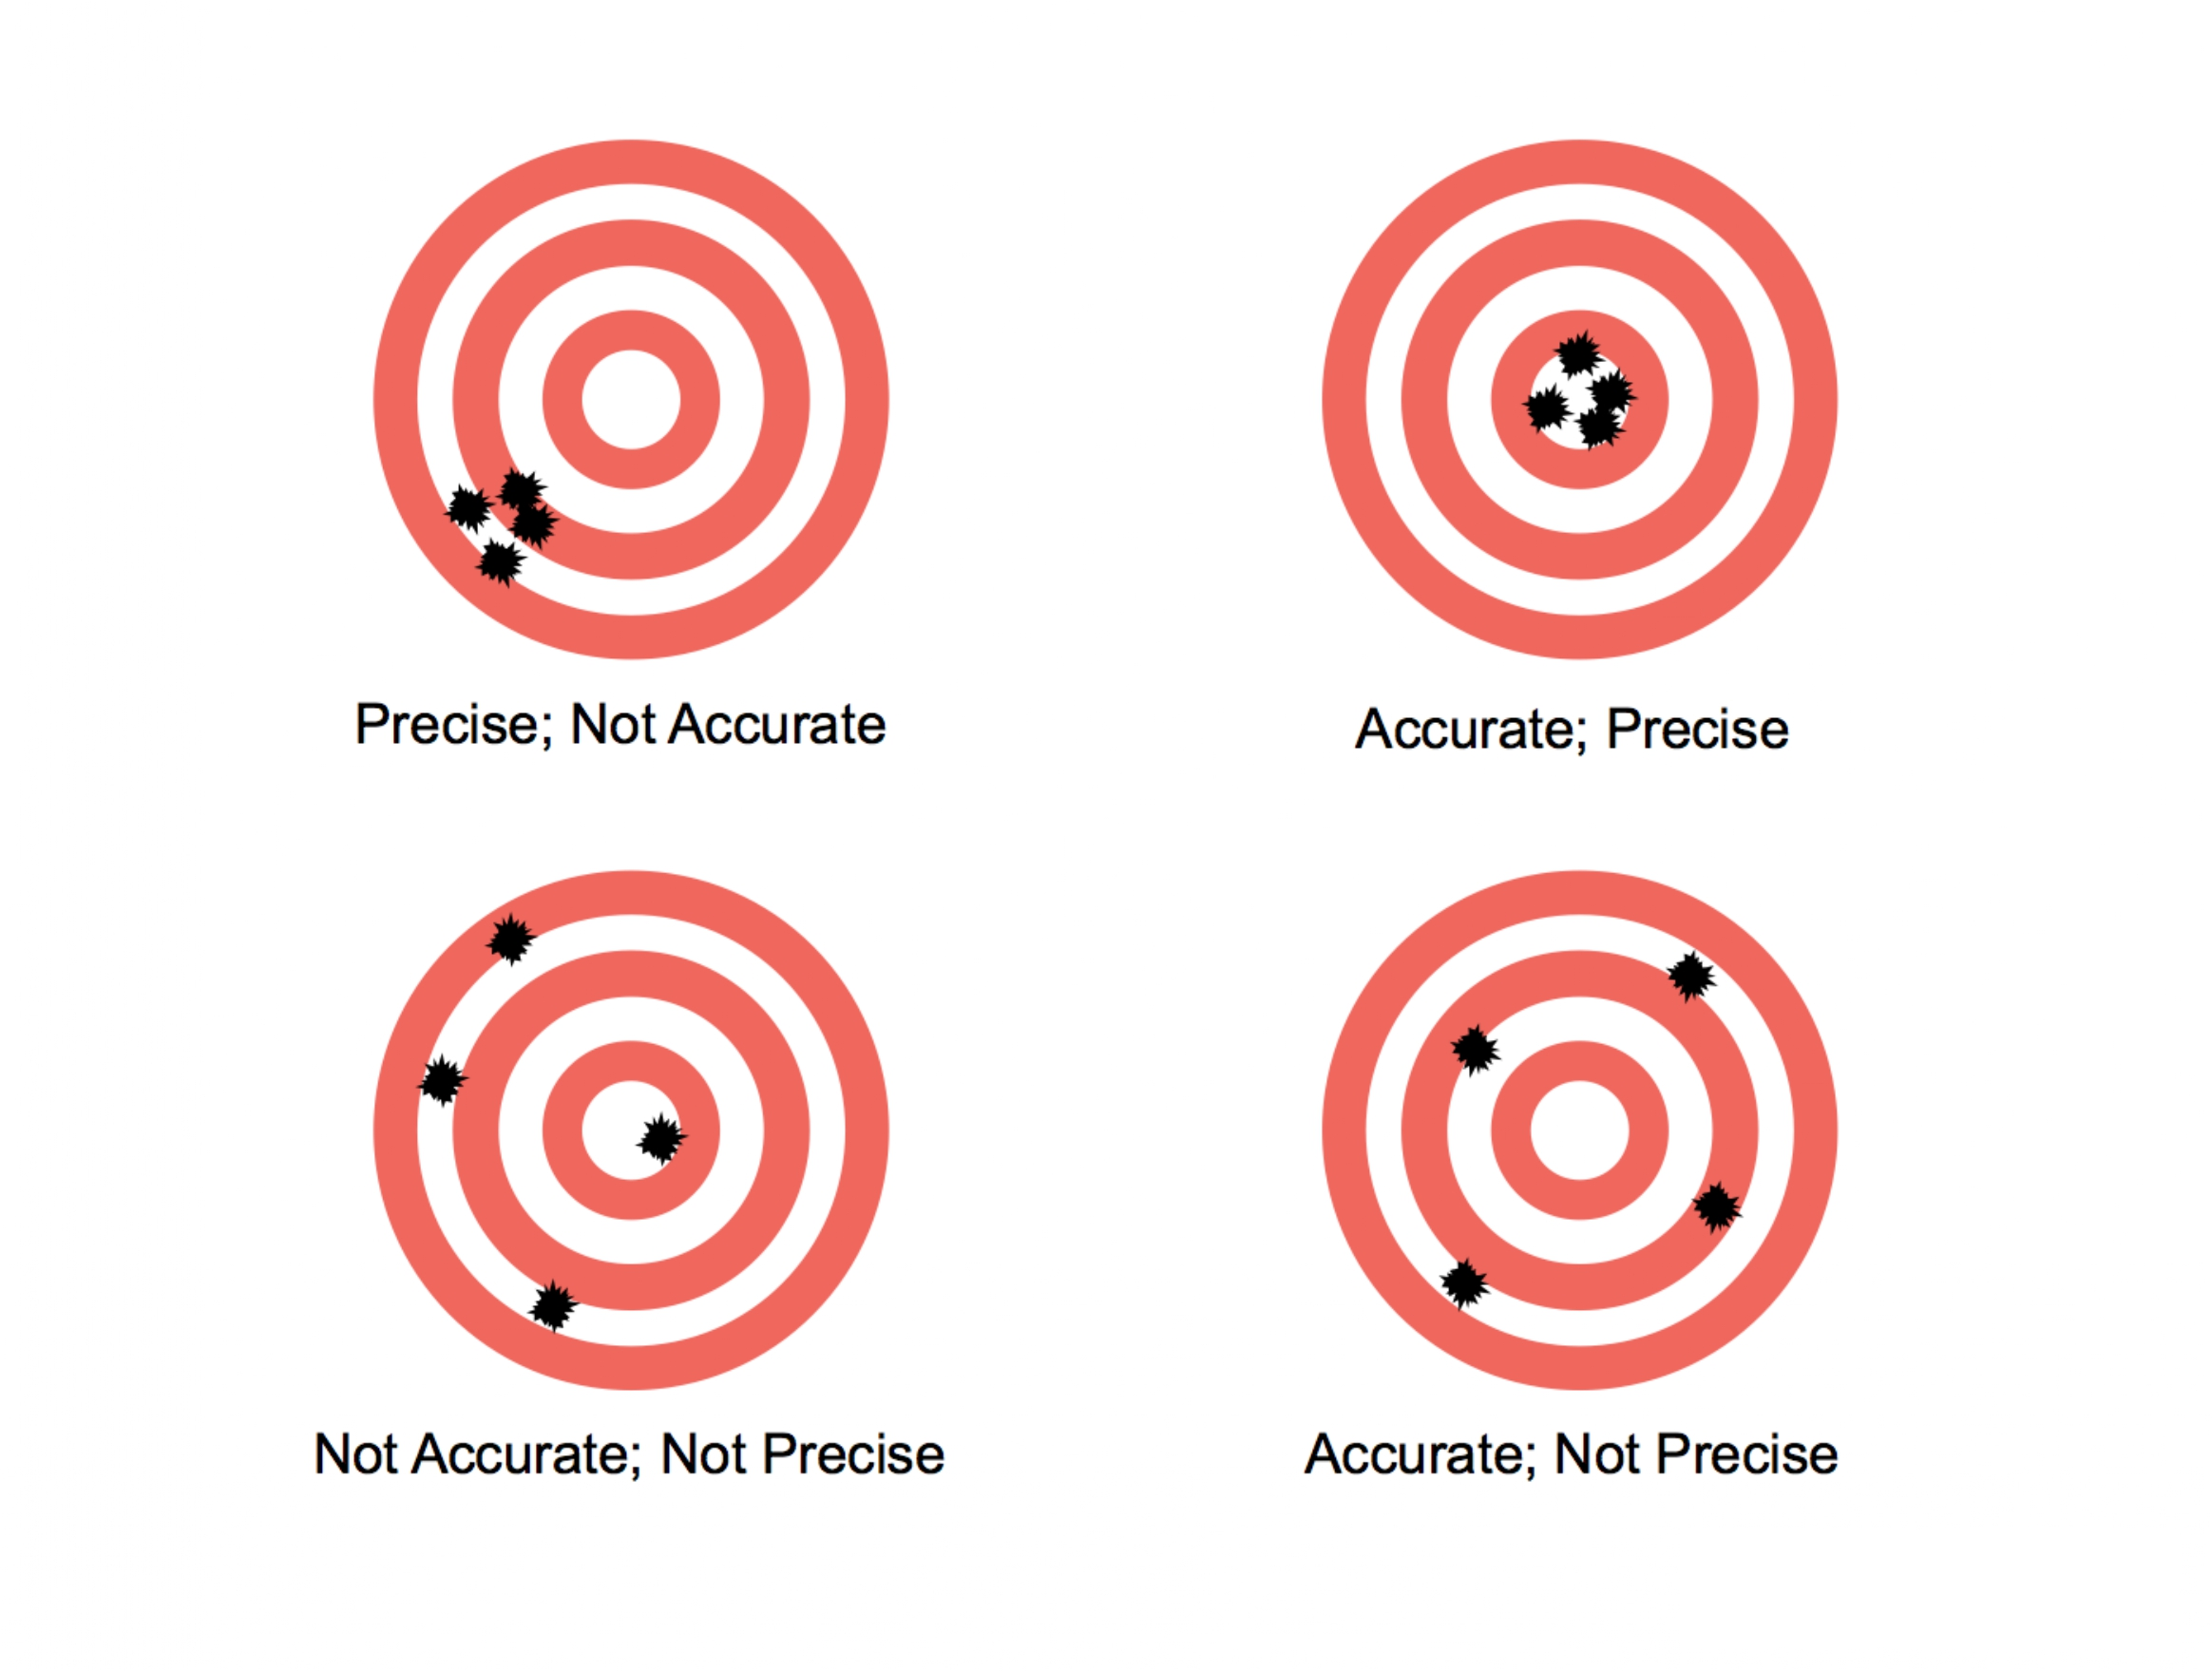
\includegraphics[width=1\linewidth]{images/unbiased} 

}

\caption{Havainnollistuksia estimaattoreiden ominaisuuksista.}\label{fig:unbiased}
\end{figure}

\begin{defblock}{}
\textbf{Tyhjentävyys}

Tyhjentävä estimaattori käyttää kaiken otokseen sisältyvän parametria \(\theta\) koskevan informaation.

\end{defblock}

\begin{defblock}{}
\textbf{Tehokkuus}

Kahdesta saman parametrin \(\theta\) estimaattorista tehokkaampi on se, jonka varianssi on pienempi. Ts. \(\widehat{\theta}^{(1)}\) on tehokkaampi kuin \(\widehat{\theta}^{(2)}\), jos \(\mathrm{Var}(\widehat{\theta}^{(1)}) \le \mathrm{Var}(\widehat{\theta}^{(2)})\).

\end{defblock}

\begin{defblock}{}
\textbf{Tarkentuvuus}

Tarkentuvan estimaattorin \(\widehat{\theta}\) arvot lähestyvät parametrin \(\theta\) oikeaa arvoa otoskoon kasvaessa.

\end{defblock}

\begin{itemize}
\tightlist
\item
  Voidaan osoittaa (yksityiskohdat sivuutetaan tällä kurssilla), että esimerkiksi yksinkertaisen satunnaisotoksen tapauksessa tavanomaisilla binomi- ja normaalijakauman parametrien estimaattoreilla on kaikki edellä mainitut hyvät ominaisuudet.

  \begin{itemize}
  \tightlist
  \item
    Näin ei ole yleisesti monimutkaisemmissa otantatilanteissa ja tilastollisisssa malleissa.
  \item
    Estimaattoreiden kehittäminen erilaisten tilastollisten mallien tapauksessa kuuluu teoreettisen tilastotieteen alaan.
  \end{itemize}
\item
  Seuraavaksi perehdytään tarkemmin kahteen kenties useimmiten tarkasteltavaan tunnuslukuun ja niiden otosjakaumiin:

  \begin{itemize}
  \tightlist
  \item
    Aritmeettisen keskiarvon otosjakaumaan \ref{alaluku63}
  \item
    Suhteellisen osuuden (frekvenssin) otosjakaumaan \ref{alaluku64}
  \end{itemize}
\end{itemize}

\hypertarget{alaluku63}{%
\section{Otoskeskiarvo ja otosvarianssi (estimaattoreina)}\label{alaluku63}}

\textbf{Otoskeskiarvo}

\begin{itemize}
\tightlist
\item
  Oletetaan, kuten aiemmin, että \(Y_1,\ldots,Y_n\) ovat riippumattomia sm:jia ja että ne muodostavat satunnaisotoksen jakaumasta, jonka odotusarvo on \(\mu\), ts. \(\text{E}(Y_i) = \mu\) ja varianssi on \(\sigma^2\), ts. \(\text{Var}(Y_i) = \sigma^2\).

  \begin{itemize}
  \tightlist
  \item
    Havaintojen (satunnaismuuttujien) \(Y_1, \ldots, Y_n\) \textbf{otoskeskiarvo} on
  \end{itemize}
\end{itemize}

\[
\bar{Y} = \frac{1}{n}(Y_1 + \cdots + Y_n) = \frac{1}{n} \sum_{i=1}^{n} Y_i
\]

\begin{itemize}
\tightlist
\item
  Yksittäisen otoksen otoskeskiarvo on tällöin sm:jien realisaatioiden aritmeettinen keskiarvo
\end{itemize}

\[
\bar{y} = \frac{1}{n} \sum_{i=1}^{n} y_i.
\]

\begin{itemize}
\tightlist
\item
  Otoskeskiarvo on satunnaismuutuja, jonka saama arvo vaihtelee satunnaisesti otoksesta toiseen johtuen satunnaisotannasta.
\item
  Kun satunnaismuuttujat ovat samoin jakautuneet odotusarvonaan \(\mu\), on otoskeskiarvo jakauman odotusarvon harhaton estimaattori, ts.
\end{itemize}

\[\text{E}(\bar{Y}) = \mu\]

\begin{itemize}
\tightlist
\item
  Täten otoskeskiarvo kuvaa aineiston perusjoukon tilastollisen mallin odotusarvoa.
\end{itemize}

\textbf{Aritmeettisen keskiarvon ominaisuuksia}

\begin{itemize}
\item
  Aiempien oletusten pätiessä aritmeettisella keskiarvolla \(\bar{Y}\) on seuraava odotusarvo ja varianssi:
  \[
  \text{E}(\bar{Y}) = \mu,  \quad
  \mathrm{Var}(\bar{Y}) = \frac{\sigma^2}{n}.
  \]
\item
  Aritmeettisen keskiarvon \(\bar{Y}\) \textbf{standardipoikkeama}
\end{itemize}

\[
\text{D}(\bar{Y}) = \sqrt{\mathrm{Var}(\bar{Y})} = \frac{\sigma}{\sqrt{n}}.
\]

\begin{itemize}
\item
  Standardipoikkeamaa kutsutaan myös \textbf{keskiarvon keskivirheeksi} ja se kuvaa otoskeskiarvon otosvaihtelua odotusarvon \(\mu\) ympärillä.
\item
  Aritmeettisen keskiarvon otosjakauma keskittyy yhä voimakkaammin havaintojen yhteisen odotusarvon \(\mu\) ympärille, kun otoskoko \(n\) kasvaa.

  \begin{itemize}
  \tightlist
  \item
    Ts. otoskoon \(n\) kasvaessa \(\mathrm{Var}(\bar{Y}) = \frac{\sigma^2}{n}\) pienenee.
  \end{itemize}
\end{itemize}

\textbf{Otosvarianssi}

\begin{itemize}
\item
  Aineiston sisältämää vaihtelua kuvataan \textbf{otosvarianssilla}
  \[
  S^2= \frac{1}{n-1} \sum_{i=1}^{n} (y_i - \bar{y})^2.
  \]

  \begin{itemize}
  \tightlist
  \item
    Vastaavasti sm:jien vaihtelua perusjoukon tasolla kuvataan \textbf{populaatiovarianssilla}
  \end{itemize}
\end{itemize}

\[
\sigma^2= \frac{1}{N} \sum_{j=1}^{N} (Y_j - \mu)^2,
\]
jota otosvarianssi harhattomasti estimoi.

\begin{itemize}
\item
  Huomioi, että \textbf{otosvarianssi} on eri asia kuin \textbf{otoskeskiarvon varianssi}.
\item
  Otoskeskiarvo \(\bar{Y}\) ja otosvarianssi \(S^2\) ovat siis satunnaismuuttujia, joiden saamat arvot vaihtelevat satunnaisesti otoksesta toiseen.
\end{itemize}

\textbf{Normaalijakautunut otos}

\begin{itemize}
\item
  Muodostakoot havainnot \(Y_1, \ldots, Y_n\) satunnaisotoksen normaalijakaumasta \(\text{N}(\mu, \sigma^2)\).
\item
  Tällöin voidaan osoittaa, että havaintojen \(Y_1, \ldots, Y_n\) keskiarvo \(\bar{Y}\) noudattaa normaalijakaumaa odotusarvolla \(\mu\) ja varianssilla \(\sigma^2/n\). Merkitään
  \[
  \bar{Y} \thicksim \text{N} \Big(\mu, \frac{\sigma^2}{n} \Big).
  \]
\item
  Itse asiassa ns. \textbf{asymptoottiseen teoriaan} vedoten (suurten otosten tapauksessa) voidaan osoittaa, että edellämainittu tulos pätee myös ilman normaalisuusoletusta.

  \begin{itemize}
  \tightlist
  \item
    Nämä tarkastelut vaativat jälleen selvästi enemmän käytyjä tilastotieteen (ja matematiikan) opintoja.
  \end{itemize}
\end{itemize}

\hfill\break

\textbf{Standardoidun aritmeettisen keskiarvon otosjakauma}

\begin{itemize}
\tightlist
\item
  Tarkastellaan \textbf{standardoitua} satunnaismuuttujaa
  \[
  Z = \frac{\bar{Y} - \text{E}(\bar{Y})}{\text{D}(\bar{Y})} = \frac{\bar{Y} - \mu}{\sigma / \sqrt{n}} = \sqrt{n} \Big(\frac{\bar{Y} - \mu}{\sigma}\Big).
  \]

  \begin{itemize}
  \tightlist
  \item
    Tällöin \(Z\):n odotusarvo \(\text{E}(Z) = 0\) ja varianssi \(\mathrm{Var}(Z) = 1\).
  \end{itemize}
\item
  Jos \(Y_i \thicksim \text{N}(\mu, \sigma^2), i=1,\ldots,n\), niin tällöin \(Z\) noudattaa standardoitua normaalijakaumaa:
  \[
  Z \thicksim \text{N}(0,1).
  \]

  \begin{itemize}
  \tightlist
  \item
    Jälleen voidaan osoittaa, että tämä tulos pätee asymptoottisesti (suurissa otoksissa) myös ilman yllä tehtyä normaalisuusoletusta.
  \end{itemize}
\end{itemize}

\hypertarget{alaluku64}{%
\section{Suhteellisen frekvenssin otosjakauma}\label{alaluku64}}

\textbf{Frekvenssi ja suhteellinen frekvenssi}

\begin{itemize}
\item
  Oletetaan, että tapahtuman \(A\) todennäköisyys on
  \[
  \text{P}(A) = p,
  \]
  jolloin tapahtuman \(A\) komplementtitapahtuman (vastatapahtuman) \(A^c\) todennäköisyys on
  \[
  \text{P}(A^c) = 1- p = q.
  \]
\item
  Poimitaan satunnaisotos, jonka koko on \(n\). Tällöin \(A\)-tyyppisten alkioiden frekvenssi eli lukumäärä kyseisessä otoksessa on \(f\).
\item
  Suhteellinen frekvenssi eli osuus on tällöin
  \[
  \widehat{p} = \frac{f}{n}.
  \]
\item
  Sekä frekvenssi (lukumäärä) \(f\) ja (täten myös) suhteellinen frekvenssi \(\widehat{p}\) ovat satunnaismuuttujia, joiden saamat arvot vaihtelevat satunnaisesti otoksesta toiseen.
\end{itemize}

\textbf{Frekvenssin otosjakauma}

\begin{itemize}
\tightlist
\item
  Frekvenssillä \(f\) on odotusarvo
  \[
  \text{E}(f) = np,
  \]
  ja varianssi
  \[
  \mathrm{Var}(f) = npq = np(1-p).
  \]
\item
  Frekvenssi \(f\) noudattaa binomijakaumaa parametrein \(n\) ja \(p\):
  \[
  f \thicksim \mathrm{Bin}(n,p).
  \]
\end{itemize}

\textbf{Suhteellinen frekvenssi: Odotusarvo ja varianssi}

\begin{itemize}
\item
  Suhteellisen frekvenssin \(\widehat{p}\) odotusarvo
  \[
  \text{E}(\widehat{p}) = \text{E} \Big(\frac{f}{n} \Big) = p,
  \]
  ja varianssi
  \[
  \mathrm{Var}(\widehat{p}) = \frac{pq}{n} = \frac{p(1-p)}{n}.
  \]
\item
  Suhteellisen frekvenssin \(\widehat{p}\) standardipoikkeamaa
  \[
  \text{D}(\widehat{p}) = \sqrt{\mathrm{Var} (\widehat{p})} =  \sqrt{\frac{pq}{n}}
  \]
  voidaan kutsua \textbf{suhteellisen frekvenssin keskivirheeksi} ja se kuvaa suhteellisen frekvenssin otosvaihtelua odotusarvon \(p\) ympärillä.
\end{itemize}

\textbf{Suhteellisen frekvenssin otosjakauma}

\begin{itemize}
\item
  Koska \(\text{E}(\widehat{p}) = p\) ja \(\mathrm{Var}(\widehat{p}) = \frac{pq}{n}\),
  niin suhteellisen frekvenssin otosjakauma keskittyy yhä voimakkaammin tapahtuman A
  todennäköisyyden \(\text{P}(A) = p\) ympärille, kun otoskoko \(n\) kasvaa.
\item
  Jälleen suurten otosten tapauksessa voidaan osoittaa, että suhteellinen frekvenssi noudattaa em. oletusten pätiessä normaalijakaumaa:
  \[
  \widehat{p} \thicksim \text{N} \Big(p, \frac{pq}{n} \Big).
  \]
\item
  Aritmeettisen keskiarvon tapaan standardoitu sm.
  \[
  Z = \frac{\widehat{p} - p}{\sqrt{\frac{pq}{n}}} \thicksim \text{N}(0,1)
  \]
  noudattaa suurissa otoksissa approksimatiivisesti standardoitua normaalijakaumaa.
\end{itemize}

\newpage

\begin{eblock}{}

\textbf{EU-kansanäänestys}

\begin{itemize}
\item
  Suomen EU-kansanäänestyksessä vuonna 1994 jäsenyyttä kannattaneiden suhteellinen osuus oli 0,54 (54 \%).
\item
  Mikä olisi ollut tällöin tn., että ennen äänestystä 200 havainnon otoksessa kyllä-osuus olisi ollut alle 50 \%?
\item
  Suhteellisen frekvenssin otosjakauman perusteella kyllä-kannatusosuuden jakauma olisi
  \[
  %\widehat{p} \stackrel{as}{\thicksim} \text{N} \Big(0.54, \frac{0.54 \times (1-0.54)}{200} \Big),
  \widehat{p} \thicksim \text{N} \Big(0.54, \frac{0.54 \times (1-0.54)}{200} \Big),
  \]
  jossa \(\frac{0.54 \times (1-0.54)}{200} = 0.0352^2\).
\item
  Näin ollen haluttu todennäköisyys (ts. saada sellainen satunnaismuuttujan \(Z \thicksim \text{N}(0,1)\) arvo että suhteellinen osuus on pienempi kuin 0.5)
  \[
  P \Big(Z < \frac{0.5-0.54}{0.0352} \Big) = P (Z < -1.14) \approx 0.127.
  \]
\end{itemize}

\end{eblock}

\hypertarget{alaluku65}{%
\section{Muita tunnuslukuja}\label{alaluku65}}

Tilastollisia analyysejä tehtäessä johtopäätösten ja objektiivisten tulkintojen tueksi tarvitaan tunnuslukuja. Mm. otoskeskiarvoa tunnuslukuna tarkasteltiin jo edellä. Tunnuslukuja on paljon, ja jokainen niistä valottaa muuttujan jakaumaa eri näkökulmista.

Jakaumien tunnusluvut voidaan jakaa sijaintilukuihin, hajontalukuihin ja muihin tunnuslukuihin. Kahdesta ensimmäisestä esimerkkejä ovat keskiarvo ja varianssi tai keskihajonta (välimatka- ja suhdeasteikon havaintojen tapauksessa). Esitellään seuraavassa vielä lyhyesti muutamia muita tunnuslukuja.

\begin{itemize}
\item
  \textbf{Moodi}: Moodi eli tyyppiarvo on havaintoaineiston yleisin muuttujan arvo tai se on luokka, jolla on suurin frekvenssi.
\item
  \textbf{Mediaani}: Mediaani on järjestetyn havaintoaineiston keskimmäinen arvo (jos havaintoarvoja on pariton määrä, parillisessa tapauksessa esitetään jompikumpi keskimmäisistä arvoista). Mediaani siis jakaa järjestetyn havaintoaineiston kahteen osaan siten, että puolet arvoista on mediaania pienempiä ja puolet arvoltaan mediaania suurempia.

  \begin{itemize}
  \tightlist
  \item
    Luokitteluasteikolla mitattaville muuttujille ei ole olemassa luontevia sijaintilukuja keskilukujen yhteydessä pl. moodi.
  \end{itemize}
\item
  Järjestysasteikolla mitatuille muuttujille voidaan mediaanin lisäksi määrittää \textbf{fraktiileja}: pp\%:n fraktiili jakaa tilastoaineiston kahteen osaan siten, että kyseistä fraktiilia pienempiä havaintoarvoja on pp\%.

  \begin{itemize}
  \tightlist
  \item
    Eniten käytettyjä fraktiileja ovat \textbf{kvartiilit}. \textbf{Alakvartiili} \(Q_1\) on 25 \%:n fraktiili, ja \textbf{yläkvartiili} \(Q_3\) on 75 \% fraktiili.
  \item
    Tietyistä fraktiileista käytetään nimitystä \textbf{desiili}. Ensimmäinen desiili \(D_1\) on 10 \% fraktiili ja esim. yhdeksäs fraktiili \(D_9\) on 90 \% fraktiili.
  \end{itemize}
\item
  Hajontalukuja: Varianssin/keskihajonnan lisäksi, jos muuttuja on mitattu vähintään järjestysasteikolla, sille voidaan määrittää vaihteluväli ja kvartiiliväli. \textbf{Vaihteluväli} kuvaa aineiston kokonaispeittoa ja siinä ilmoitetaan aineiston pienin havainto ja suurin havainto. Ts. vaihteluväli=(pienin havainto, suurin havainto). \textbf{Kvartiiliväli} = (\(Q_1, Q_3\)).
\item
  Muita tunnuslukuja: Tilastollisen päätöksenteon yhteydessä käytettäviä tunnuslukuja ovat \textbf{vinous} ja \textbf{huipukkuus}. Vinous ja huipukkuus voidaan määrittää välimatka- ja suhdeasteikon muuttujille. Vinous ja huipukkuus mittaavat kumpikin omalla tavallaan jakauman poikkeamaa normaalijakaumasta. Normaalijakauman vinous on 0 ja huipukkuus on 3.
\end{itemize}

\hypertarget{alaluku66}{%
\section{Luottamusvälit}\label{alaluku66}}

\begin{itemize}
\tightlist
\item
  Satunnaisesti saadusta aineistosta laskettujen tunnuslukujen luotettavuus on tilastollisen mallin parametrien estimoinnissa keskeinen tilastollinen kysymys.

  \begin{itemize}
  \tightlist
  \item
    Otoksen poimintaan liittyvän satunnaisvaihtelun vuoksi emme voi varmuudella tietää onko saatu otokseen perustuva parametriestimaatti ``lähellä'' vai ``kaukana'' sen todellisesta arvosta.
  \item
    Täten tarvitaan jokin tapa, jolla saadun parametriestimaatin luotettavuutta voidaan arvioida.
  \end{itemize}
\end{itemize}

\begin{defblock}{}
\textbf{Luottamusväli}

Luottamusväli on otoksen perusteella määrätty väli, joka tutkijan valitsemalla todennäköisyydellä (luottamustasolla) peittää tarkasteltavan tilastollisen mallin \(f(y;\theta)\) parametrin \(\theta\) tuntemattoman todellisen arvon. Se perustetaan otostunnusluvun, estimaattorin, otosjakaumaan.

\end{defblock}

\begin{itemize}
\item
  Otoskoko on luottamusvälejä koskevissa tarkasteluissa keskeinen ja luottamusväleihin palataankin otoskoon käsittelyn yhteydessä.
\item
  Valittua luottamustasoa merkitään usein \(1-\alpha\):lla, jossa \textbf{merkitsevyystaso} (\textbf{riskitaso}) \(\alpha\) on esimerkiksi \(\alpha=0.05\).
\item
  Tulkinta: Jos \textbf{otantaa} jakaumasta \(f(y;\theta)\) toistetaan, niin keskimäärin \(100 \times (1-\alpha)\%\) otoksista konstruloiduista luottamusväleistä peittää parametrin \(\theta\) todellisen arvon.
\item
  Oletetaan, että olemme tehneet johtopäätöksen, että konstruloitu luottamusväli peittää parametrin \(\theta\) tuntemattoman todellisen arvon.

  \begin{itemize}
  \tightlist
  \item
    Tällöin otantaa toistettaessa luottamusvälin konstruktiosta seuraa, että tehty johtopäätös on oikea keskimäärin \(100 \times (1-\alpha)\%\) tapauksista.
  \item
    Vastaavasti taas \(100 \times \alpha \%\) ei peitä parametrin todellista arvoa.
  \end{itemize}
\item
  Luottamusväli on kenties tunnetumpi kansankieliseltä nimitykseltään \textbf{virhemarginaali}, joka on itse asiassa luottamusvälin puolikas: todellinen parametriarvo kuuluu saadun estimaatin ja virhemarginaalien sisään jäävälle osuudelle.

  \begin{itemize}
  \tightlist
  \item
    Normaalisti mm. otoskoon kasvu pienentää virhemarginaalia.
  \item
    Kuten jatkossa tullaan havaitsemaan, virhemarginaalin suuruuteen vaikuttavat otosasetelma, otoskoko, luottamustaso ja tutkittavan tilastollisen tunnusluvun jakauma.
  \end{itemize}
\item
  Luottamusväleissä ei varsinaisesti ole kyse ``virheestä'' vaan saadun/muodostetun tiedon tarkkuudesta.

  \begin{itemize}
  \tightlist
  \item
    Luottamusvälit, eli virhemarginaalit, siis (yleisesti) riippuvat valittavasta luottamustasosta \(1-\alpha\) ja näin ollen samasta aineistosta on saatavissa useita virhemarginaaleja.

    \begin{itemize}
    \tightlist
    \item
      Täten on tarkalleen ottaen virheellistä sanoa, että ``tutkimuksen virhemarginaali on 3,5 puoleen tai toiseen''.
    \item
      Oikeammin olisi sanoa esimerkiksi ``tutkimuksessa saadun kannatuksen virhemarginaali on 3,5 puoleen tai toiseen 95 \% luottamustasolla.''
    \item
      Virhemarginaali kasvaa, kun aineistoa lohkotaan: jos tuhannen hengen otoksesta esitetään tietoja, jotka kuvaavat erikseen miesten ja naisten ominaisuuksia, sukupuolittain lasketut ovat estimaatit epävarmempia kuin koko otoksesta esitetyt.
    \end{itemize}
  \item
    Vastaavasti on virheellistä sanoa että tutkimuksella olisi virhemarginaali, sillä virhemarginaali liittyy aina vain tutkimuksen antamiin numeerisiin arvoihin.
  \item
    Aitoja virhelähteitä ovat mm. otantatutkimukseen liittyvien kysymysten muotoilu, käsitteiden monitulkintaisuus, vastaajien valikoituminen ja vastauskato.
  \end{itemize}
\end{itemize}

\textbf{Normaalijakauman odotusarvon luottamusväli}

\begin{itemize}
\item
  Käsittelemme seuraavassa (normaalijakauman) odotusarvon \(\mu\) luottamusvälejä ja jatkossa oletetaan (ellei toisin mainita), että taustalla oleva populaatio, \(N\), on ``iso'' (ääretön).

  \begin{itemize}
  \tightlist
  \item
    Näin ollen ns. äärellisyyskorjausta ei käytetä (yksinkertaisuuden vuoksi).
  \end{itemize}
\item
  Tarkastellaan satunnaisotosta normaalijakaumasta
  \(Y_1, \ldots, Y_n \perp \!\!\! \perp, \,\, Y_i \thicksim \text{N}(\mu, \sigma^2),\, i=1,\ldots,n\).
\item
  Tarkastellaan normaalijakauman odotusarvon \(\mu\) luottamusvälin määräämistä otannan avulla olettaen että jakauman varianssi \(\sigma^2\) on tunnettu.

  \begin{itemize}
  \tightlist
  \item
    Muistetaan että normaalijakauman odotusarvoparametrin \(\text{E}(Y_i) = \mu\) \textbf{harhaton estimaattori} on aritmeettinen keskiarvo
  \end{itemize}
\end{itemize}

\[
\bar{Y} = \frac{1}{n} \sum_{i=1}^{n} Y_i.
\]

\begin{itemize}
\item
  Valitaan \textbf{luottamustasoksi} \(1-\alpha\), eli \(\alpha\) määrää todennäköisyyden, jolla luottamusväli peittää odotusarvon \(\mu\) todellisen arvon: yleinen valinta ihmistieteissä on \(\alpha = 0.05\) tai \(\alpha = 0.1\) vastaten 95\% ja 90\% prosentin luottamustasoa. Luonnontieteissä \(\alpha\) on usein paljon pienempi.
\item
  Määrätään \textbf{luottamuskertoimet} \(-z_{\alpha/2}\) ja \(z_{\alpha/2}\) (luottamusväli on kaksisuuntainen), joille pätee
  \[
  \text{P}(-z_{\alpha/2} \le Z \le z_{\alpha/2}) = 1-\alpha,
  \]
  jossa standardoitu satunnaismuuttuja
  \[
  Z = \frac{\bar{Y} - \mu}{\sigma / \sqrt{n}} = \sqrt{n} \Big( \frac{\bar{Y} - \mu}{\sigma} \Big),  
  \]
  (ks. aiemmat alaluvut tässä luvussa \ref{luku6}) noudattaa \(\text{N}(0,1)\)-jakaumaa.

  \begin{itemize}
  \tightlist
  \item
    \(\text{P}(\cdot)\):llä merkitään todennäköisyyttä, joka tässä tapauksessa liittyy normaalijakaumaan, ja \(z_{\alpha/2}\) on jakaumafunktion arvo pisteessä \(\alpha/2\).
  \end{itemize}
\item
  Tällöin etsitään odotusarvoparametrille \(\mu\) sellainen arvo, jolla oheinen epäyhtälö pätee ja päädytään luottamusväliin.
\item
  Nyt epäyhtälöketju voidaan kirjoittaa muodossa
  \[
  -z_{\alpha/2} \le  \frac{\bar{Y} - \mu}{\sigma / \sqrt{n}}  \le z_{\alpha/2}.
  \]
\item
  Joka voidaan kirjoittaa uudelleen muodossa
  \[
  \bar{Y} - z_{\alpha/2} \frac{\sigma}{\sqrt{n}} \le   \mu  \le 
  \bar{Y} + z_{\alpha/2} \frac{\sigma}{\sqrt{n}},
  \]
  kertomalla nimittäjällä puolittain ja vähentämällä sm:jien keskiarvo molemmin puolin.
\item
  Normaalijakauman odotusarvon \((1-\alpha) \times 100\)\% luottamusväli on siis
  \[
  \Big(\bar{Y} - z_{\alpha/2} \frac{\sigma}{\sqrt{n}}, 
  \bar{Y} + z_{\alpha/2} \frac{\sigma}{\sqrt{n}} \Big).
  \]
\item
  Luottamusväli on symmetrinen keskipisteensä \(\bar{Y}\) suhteen. Siksi luottamusväli esitetään usein
  \[
  \bar{Y} \pm z_{\alpha/2} \frac{\sigma}{\sqrt{n}}.
  \]
\item
  Luottamusvälin pituus
  \[
  2 \cdot z_{\alpha/2} \frac{\sigma}{\sqrt{n}}.
  \]
\item
  \textbf{Virhemarginaali} on luottamusvälin pituuden puolikas eli
  \[
  z_{\alpha/2} \frac{\sigma}{\sqrt{n}}.
  \]
\item
  Edellä tiettyyn otokseen liittyvä luottamusväli perustetaan realisoituneeseen otoskeskiarvoon \(\bar{y}=\frac{1}{n} \sum_{i=1}^{n} y_i\).
\item
  Olisi toivottavaa pystyä konstruoimaan parametrille \(\mu\) mahdollisimman lyhyt luottamusväli, johon liittyvä luottamustaso olisi samanaikaisesti mahdollisimman korkea. Molempien vaatimusten samanaikainen täyttäminen ei ole kuitenkaan mahdollista, jos otoskoko \(n\) pidetään kiinteänä:

  \begin{itemize}
  \tightlist
  \item
    Luottamustason kasvattaminen pidentää luottamusväliä, jolloin tieto parametrin \(\mu\) todellisesta arvosta tulee epätarkemmaksi.
  \item
    Luottamusvälin lyhentäminen pienentää luottamustasoa, jolloin tieto parametrin \(\mu\) todellisesta arvosta tulee epävarmemmaksi.
  \end{itemize}
\end{itemize}

\begin{figure}

{\centering 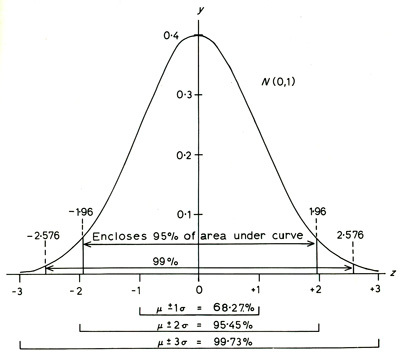
\includegraphics[width=1.5\linewidth]{images/gaussian-distribution} 

}

\caption{Standardoitu normaalijakauma: Virhemarginaaleja}\label{fig:foo}
\end{figure}

\hfill\break

\textbf{Normaalijakauman odotusarvon luottamusväli (\(\sigma^2\) tuntematon)}

\begin{itemize}
\item
  Tarkastellaan edelleen satunnaisotosta normaalijakaumasta, mutta oletetaan nyt että varianssi \(\sigma^2\) tuntematon.
\item
  Normaalijakauman odotusarvon \((1-\alpha) \times 100\)\% luottamusväli:
  \[
  \Big(\bar{Y} - t_{\alpha/2} \frac{S}{\sqrt{n}}, 
  \bar{Y} + t_{\alpha/2} \frac{S}{\sqrt{n}} \Big),
  \]
  jossa \textbf{luottamuskertoimet} \(-t_{\alpha/2}\) ja \(t_{\alpha/2}\)
  saadaan nyt \(t\)\textbf{-jakaumasta} \(t_{n-1}\), jossa \(S^2\) on varianssin \(\sigma^2\) harhaton estimaattori ja vapausasteiden lukumäärä on \(n-1\).

  \begin{itemize}
  \item
    (Studentin) \(t\)-jakauma muistuttaa silmämääräisesti normaalijakaumaa, mutta se on paksuhäntäisempi. Vapausasteluvun kasvaesssa \(t\)-jakauma lähestyy normaalijakaumaa.
  \item
    Suurissa otoksissa (\(n\) iso) luottamuskertoimet voidaan poimia (approksimatiivisesti) myös normaalijakaumasta eli korvata edellä kertoimet \(t_{\alpha/2}\) aiemmin käytetyillä kertoimilla \(z_{\alpha/2}\).
  \item
    Normaalijakauman odotusarvon luottamusväli (\(\sigma^2\) tuntematon), \(t\)-jakauma eri vapausastein \(df\)
  \end{itemize}
\end{itemize}

\begin{figure}

{\centering 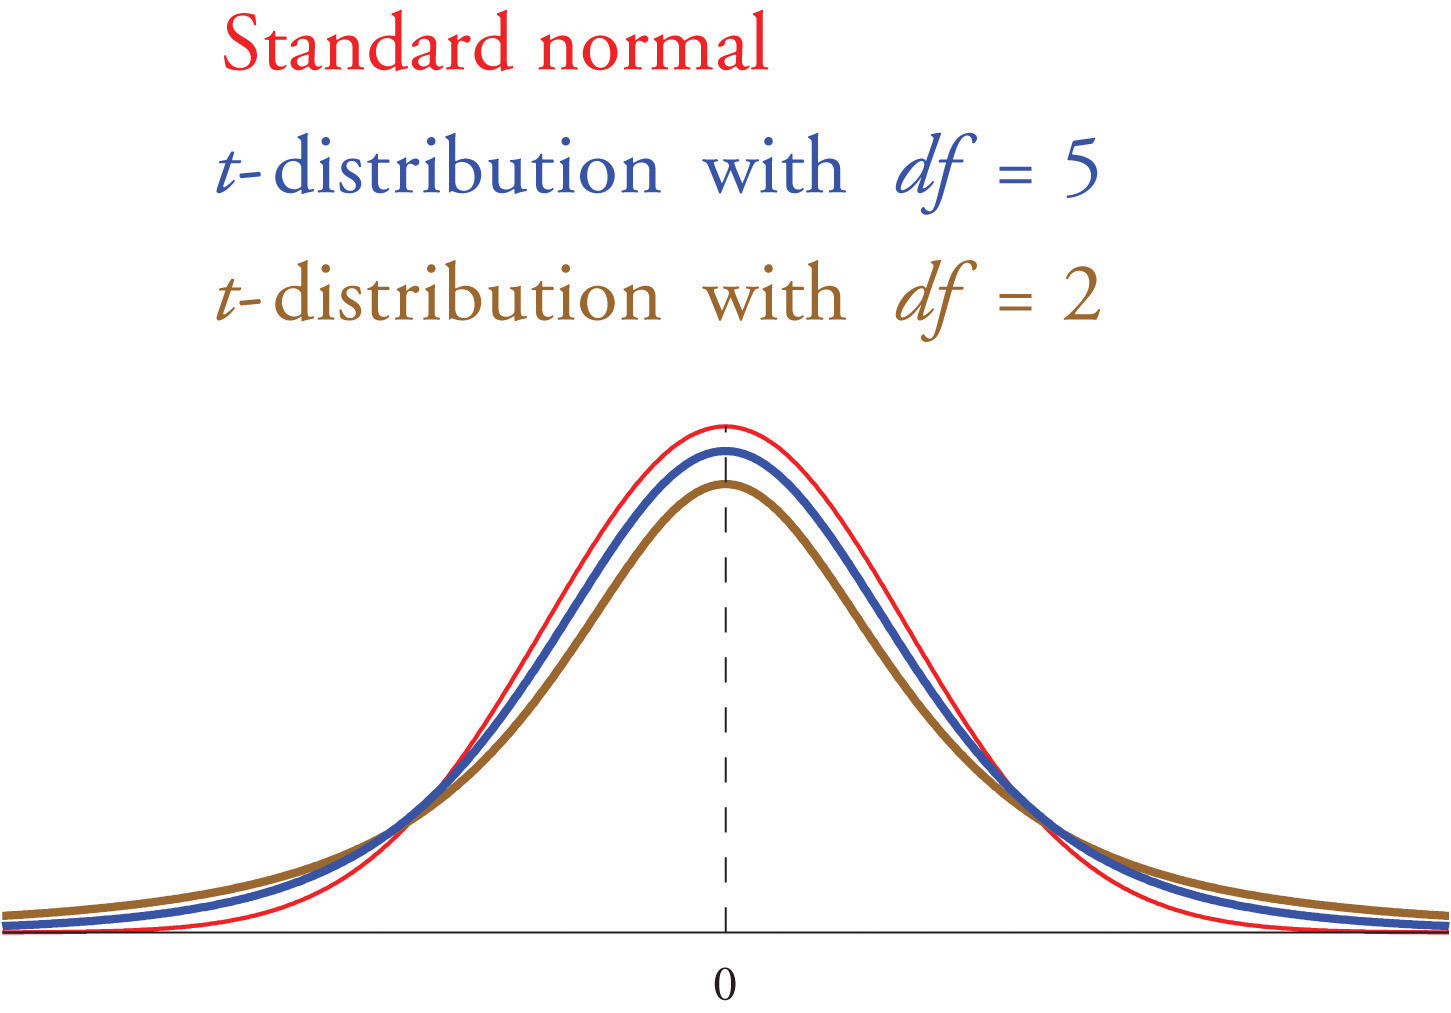
\includegraphics[width=0.75\linewidth]{images/NjaT-jakauma} 

}

\caption{t-jakauman (ja standardoidun normaalijakauman) tiheysfunktioita}\label{fig:unnamed-chunk-7}
\end{figure}

\hfill\break

\textbf{Luottamusväli: Suhteellisen osuuden odotusarvo}

\begin{itemize}
\item
  Käsittelemme seuraavassa suhteellisen osuuden \(p\) luottamusvälejä.
\item
  Tarkastellaan satunnaisotosta Bernoulli-jakaumasta
  \(Y_1, \ldots, Y_n \perp \!\!\! \perp, \,\, Y_i \thicksim B(p),\, i=1,\ldots,n\),
  jossa merkitään \(Y_i=1\) jos tapahtuma A tapahtuu ja \(Y_i=0\) jos tapahtuma A ei tapahdu.
\item
  Bernoulli-jakauman odotusarvoparametrin \(p=\text{E}(Y_i)\) harhaton estimaattori on tapahtuman A suhteellinen otosfrekvenssi
  \[
  \widehat{p} = \frac{1}{n} \sum_{i=1}^{n} Y_i.
  \]
\item
  Bernoulli-jakauman (vrt. binomijakauma) ominaisuuksien
  perusteella \(\text{E}(Y_i)=p\) ja \(\mathrm{Var}(Y_i)=pq\), jossa
  \(q=1-p\).
\item
  Näin ollen voimme normaalijakauman odotusarvoparametrin
  luottamusvälin konstruloinnin tapaan määritellä satunnaismuuttujan \(Z\):
  \[
  Z = \frac{\widehat{p} - p}{\sqrt{\frac{p (1-p)}{n}}} = 
  \sqrt{n} \Big(\frac{\widehat{p} - p}{\sqrt{p (1-p)}} \Big),  
  \]
  joka noudattaa (suurissa otoksissa) \(\text{N}(0,1)\)-jakaumaa.
\item
  Suhteellisen frekvenssin hajonnan estimaattori on siis
  \[
  \sqrt{\frac{\widehat{p} (1-\widehat{p})}{n}},
  \]
  jossa tuntematon \(p\) on korvattu sen estimaattorilla (otosvastineella) \(\widehat{p}\).
\item
  Luottamuskertoimet määrätään aiempaan tapaan:
  \[
  \text{P}(-z_{\alpha/2} \le Z \le z_{\alpha/2}) = 1-\alpha,
  \]
\item
  Näin ollen odotusarvoparametrin (suhteellisen osuuden) \(p\) \((1-\alpha)\)\% luottamusväliksi
  saadaan
  \[
  \Big(
  \widehat{p} - z_{\alpha/2} \sqrt{\frac{\widehat{p}(1-\widehat{p})}{n}},
  \widehat{p} + z_{\alpha/2} \sqrt{\frac{\widehat{p}(1-\widehat{p})}{n}} 
  \Big)
  \]
\item
  Luottamusväli voidaan kirjoittaa
  \[
  \widehat{p} \pm z_{\alpha/2} \sqrt{\frac{\widehat{p}(1-\widehat{p})}{n}}
  \]
  ja luottamusvälin pituus on
  \[
  2 \times z_{\alpha/2} \sqrt{\frac{\widehat{p}(1-\widehat{p})}{n}}.
  \]
\end{itemize}

\hypertarget{alaluku67}{%
\section{Otoskoko}\label{alaluku67}}

\begin{itemize}
\tightlist
\item
  Yksi tilastollisen päättelyn keskeisiä tavoitteita on yleistää otoksen pohjalta tehty päättely koskemaan koko perusjoukkoa. Seuraavaksi käymme läpi seikkoja, jotka tulee ottaa huomioon otoskokoa miettiessä.
\item
  Kun on päätetty, millainen tutkimusaineisto halutaan kerätä, on päätettävä, kuinka suuri otoksen on oltava, jotta se edustaa tutkittavaa joukkoa kattavasti.

  \begin{itemize}
  \tightlist
  \item
    Liian pieni \textbf{otoskoko}, eli pieni määrä otokseen poimittuja tilastoyksiköitä, voi \textbf{sattumalta} poiketa paljonkin perusjoukosta.

    \begin{itemize}
    \tightlist
    \item
      Tämä niin kutsuttu \textbf{otantavirhe} on sitä suurempi mitä pienempää otosta käytetään.
    \item
      Liian pienen otoksen vuoksi muuten hyvin toteuttu tutkimus- ja otanta-asetelma saattaa epäonnistua vastaamaan tutkimuksen mielenkiinnon kohteena olevaan kysymykseen.
    \end{itemize}
  \item
    Todella suuren otoksen koostaminen voi olla \textbf{työlästä}, \textbf{kallista} tai joskus jopa \textbf{täysin mahdotonta} esimerkiksi siksi että käytettävissä olevat tutkimusyksiköt eivät ole käytettävissä ajallisten rajoitteiden vuoksi (kuten harvinaisten tautien kantajat).

    \begin{itemize}
    \tightlist
    \item
      Toisaalta perusjoukon systemaattiset piirteet tulevat otoskoon kasvaessa paremmin esille, vaikka yksittäisten otosyksiköiden tilastolliset muuttujat saattavat vaihdella suuresti.
    \end{itemize}
  \item
    \textbf{Otoskoko} siis vaikuttaa keskeisesti siihen, miten hyvin otoksesta tehdyt johtopäätökset voidaan yleistää koskemaan koko perusjoukkoa!
  \end{itemize}
\item
  Optimaalinen, tai ainakin tutkimusongelmaan vastaamisen kannalta vähintään riittävä arvio, otoskoosta voidaan usein määrätä etukäteen.
\end{itemize}

\hfill\break

\textbf{Perusjoukon rooli otoskoon määrittämisessä}

\begin{itemize}
\tightlist
\item
  Ensiksi tulee kuitenkin pohtia käsillä olevaa tutkimusongelmaa esimerkiksi kysymällä: \textbf{Millainen on perusjoukkosi?}

  \begin{itemize}
  \tightlist
  \item
    Onko tutkittavan muuttujan arvoissa paljon vaihtelua? Jos on, niin tämä täytyy huomioida kasvattamalla otoskokoa.

    \begin{itemize}
    \tightlist
    \item
      Esimerkiksi otosten keskiarvot alkavat käyttäytyä riittävän siististi vasta noin otoskoosta \(n=30\) alkaen.
    \item
      Kyseinen otoskoko ei kuitenkaan ole missään tapauksessa yleinen ja pätevä peukalosääntö otoskoon koolle, vaan se tulee aina päättää tutkimusongelmakohtaisesti.
    \end{itemize}
  \item
    Kuuluuko tutkimukseesi esimerkiksi otoksen sisällä olevien ryhmien keskiarvojen vertailua tai muita otoksen osajoukkojen tunnuslukujen vertailua? Jos kuuluu, niin otoskoko tulee valita pienimmän ryhmäkoon mukaan, jotta siitäkin saadaan tarpeeksi edustajia.

    \begin{itemize}
    \tightlist
    \item
      Mitä isompaa otosta käytetään, sitä pienempi perusjoukossa esiintyvä ryhmien välinen ero pystytään otoksella tunnistamaan.
    \end{itemize}
  \end{itemize}
\end{itemize}

\textbf{Tulosten vaaditun tarkkuuden vaikutus otoskokoon}

\begin{itemize}
\tightlist
\item
  Tarkastelemme pian esimerkin avulla, kuinka tarvittavaa otoskokoa voidaan approksimoida tulosten halutun tarkkuuden avulla.
\item
  Tarkastellaan kuitenkin ensin minkälaiset kysymykset liittyvät otoskoon pohdintaan tulosten tarkkuuden osalta.

  \begin{itemize}
  \tightlist
  \item
    Kuinka varma sinun on oltava, että tulokset vastaavat joukon mielipiteitä? Tämä on virhemarginaalisi.

    \begin{itemize}
    \tightlist
    \item
      Esimerkiksi puoluekannatuksen arvioimiseen 2 \% virhemarginaalilla riittää huomattavasti pienempi otoskoko kuin 0.2 \% virhemarginaalilla. Politiikan tutkija voisikin kasvattaa otoskokoa vaalien lähestyessä, mikäli mielii saada tarkempia tuloksia.
    \end{itemize}
  \item
    Kuinka varma haluat olla, että otos edustaa joukkoa oikein? Tämä on luottamustaso.

    \begin{itemize}
    \tightlist
    \item
      Luottamustaso on todennäköisyys sille, että valitsemasi otos on tulosten kannalta oleellinen.
    \item
      Jos joukosta poimitaan 30 otosta sattumanvaraisesti, kuinka usein yhdestä otoksesta saadut tulokset eroavat merkittävästi muista 30 otoksesta? Jos luotettavuustaso on 95 \%, samat johtopäätelmät saadaan 95 prosentissa tapauksista.
    \end{itemize}
  \end{itemize}
\end{itemize}

\textbf{Odotetun vastauskadon vaikutus otoskokoon}

\begin{itemize}
\tightlist
\item
  Kuinka suuri vastauskato tulee mahdollisesti olemaan?

  \begin{itemize}
  \tightlist
  \item
    Yleensä osa kyselytutkimukseen valituista jättää vastaamatta. Tätä kutsutaan kadoksi. Kato vinouttaa otosta, jos vastaamatta jättäneet ovat mielipiteiltään erilaisia kuin vastanneet.
  \item
    Otoskoon kasvattaminen ei paranna kadon aiheuttamaa vinoutumista.
  \end{itemize}
\item
  Esimerkki: Jos Alkon myymälän asiakastutkimus suoritetaan ovensuukyselynä maanantaina aamupäivällä, niin vastaajat eivät luultavasti edusta myymälän koko asiakaskuntaa. Otantakehikko on tässä liian suppea ja seurauksena on todennäköisesti vinoutunut otos. Vinoutuma ei korjaannu vaikka otosta kasvatetaan maanantai-aamupäivän asiakkailla.
\end{itemize}

\hfill\break

\begin{eblock}{}

\textbf{Esimerkki: otoskoko normaalijakauman odotusarvon estimoinnissa}

\begin{itemize}
\item
  Palautetaan mieleen normaalijakauman \(\text{N}(\mu,\sigma^2)\) odotusarvon luottamusvälin määrääminen (kun varianssi \(\sigma^2\) oletetaan tunnetuksi).
\item
  Luottamusväliksi saatiin
  \[
  \bar{Y} \pm z_{\alpha/2} \frac{\sigma}{\sqrt{n}},
  \]
  ja luottamusvälin symmetrisyydestä johtuen luottamusvälin pituus
  \[
  2 \times z_{\alpha/2} \frac{\sigma}{\sqrt{n}}.
  \]
\item
  Oletetaan, että normaalijakauman odotusarvoparametrille \(\mu\) halutaan konstruoida luottamusväli, jonka toivottu pituus on \(2d\) (huom. symmetrisyys).
\item
  Luottamusvälin lausekkeesta saadaan täten järjestelemällä
  \[
  n = \Big(\frac{z_{\alpha/2} \, \sigma}{d} \Big)^2.
  \]
\item
  Jos varianssi \(\sigma^2\) on tuntematon, se voidaan kaavassa korvata havaitulla otosvarianssilla \(s^2\), jolloin
  \[
  n = \Big(\frac{z_{\alpha/2} \, s}{d} \Big)^2.
  \]
\item
  Pitäydytään (yksinkertaisuuden vuoksi) luottamuskertoimissa \(z_{\alpha/2}\) vaikka varianssi \(\sigma^2\) olisikin tuntematon.
\end{itemize}

\end{eblock}

\begin{eblock}{}

\textbf{Esimerkki: otoskoko}

\begin{itemize}
\item
  Oletetaan, että haluamme määrätä otoskoon niin, että otoskeskiarvo poikkeaa populaatiokeskiarvosta korkeintaan yhden yksikön (\(d = 1\)) todennäköisyydellä \(0.05\). Oletetaan, että varianssi on aiemmissa tutkimuksissa ollut \(\sigma^2 = 5\). Oletetaan lisäksi, että taustallaoleva perusjoukko on iso (ääretön).
\item
  Tällöin otoskoon tulisi olla
  \[
  n \ge \Big(\frac{z_{\alpha/2} \, \sigma}{d} \Big)^2 = \Big(1.96 \sqrt{5} \Big)^2 \approx 19.2.
  \]
\item
  Tarvittavan otoskoon tulisi siis olla tässä tapauksessa noin 20.
\end{itemize}

\end{eblock}

\textbf{Äärellisyyskorjaus}:

\begin{itemize}
\item
  Äärellisyyskorjausta käytetään, jos otos poimitaan äärellisestä perusjoukosta palauttamatta ja (nyrkkisääntönä)
  \[
  \frac{n}{N} > 0.05,
  \]
  jossa \(n\) on edelleen otoskoko, \(N\) perusjoukon koko ja \(n < N\).
\item
  Jos suhde \(n/N\) on lähellä arvoa 1, tarkoittaa se, että perusjoukosta
  huomattava osa kuuluu otokseen.

  \begin{itemize}
  \tightlist
  \item
    Tällöin otoskeskiarvon poikkeama populaatiokeskiarvosta on luonnollisesti pienempi kuin pienemmän otoksen tilanteessa.
  \item
    Otoskoon kasvattaminen lisää siis estimoinnin tarkkuutta, ja juuri äärellisyyskertoimen avulla hajonta ``korjataan'' vastaamaan käytettyä otoskokoa.
  \end{itemize}
\end{itemize}

\textbf{Otoskoko, äärellisyyskorjaus: Normaalijakauman odotusarvon estimointi}

\begin{itemize}
\item
  Oletetaan, että otannan taustalla oleva perusjoukko on äärellinen (pieni).
\item
  Tällöin luottamusvälin konstruloinnissa huomioidaan äärellisyyskorjaus
  (vrt. aiemmat kaavat):
  \[
  \bar{Y} \pm z_{\alpha/2} \sqrt{\Big(\frac{N-n}{N}\Big)\frac{\sigma^2}{n}}.
  \]
\item
  Tarvittava otoskoko on tällöin välivaiheiden jälkeen
  \[
  n =\frac{1}{\frac{d^2}{z^2_{\alpha/2} \sigma^2} + \frac{1}{N}}.
  \]
\end{itemize}

\hfill\break

\begin{eblock}{}

\textbf{Esimerkki: otoskoko (jatkoa)}

\begin{itemize}
\item
  Oletetaan aiemman esimerkin tilanne kuitenkin siten, että perusjoukon koko on nyt \(N=100\).
\item
  Tällöin otoskooon tulisi olla
  \[
  n  \ge \frac{1}{\frac{1}{1.96^2 \times 5} + \frac{1}{100}} \approx 16.11.
  \]
\item
  Tarvittava otoskoko on siis noin 17.
\end{itemize}

\end{eblock}

\hfill\break

\textbf{Otoskoko: Suhteellinen osuus}

\begin{itemize}
\tightlist
\item
  Palautetaan mieleen Bernoulli-jakauman odotusarvoparametrin \(p\) luottamusvälin muodostaminen.

  \begin{itemize}
  \tightlist
  \item
    Kuten normaalijakauman odotusarvoparametrin tapauksessa, pyrimme muodostamaan mahdollisimman lyhyen luottamusvälin, johon liittyvä luottamustaso olisi samanaikaisesti mahdollisimman korkea.
  \end{itemize}
\item
  Oletetaan aiempaan tapaan, että \(p\):lle halutaan muodostaa luottamusväli, jonka toivottu pituus on \(2d\).
\item
  Tarvittava otoskoko saadaan kaavasta (kun perusjoukko oletetaan äärettömäksi)
\end{itemize}

\[
n = \Big(\frac{z_{\alpha/2} \,\, \sqrt{p(1-p)}}{d} \Big)^2.
\]

\hfill\break
\hfill\break

\textbf{Suhteellinen osuus, äärellisyyskorjaus:}

\begin{itemize}
\tightlist
\item
  Tarvittava otoskoko saadaan äärellisyyskorjausta käytettäessä kaavasta
  \[
  n = \frac{N p (1-p)}{\frac{(N-1) d^2}{z^2_{\alpha/2}} + p(1-p)}.
  \]

  \begin{itemize}
  \tightlist
  \item
    Voidaan osoittaa, että jos perusjoukko \(N\) on iso (ääretön), niin tällöin edellinen lauseke supistuu aiempaan otoskokoa osoittavaan lausekkeeseen.
  \end{itemize}
\item
  Usein otoskokoa määrättäessä suhteellisesta osuudesta ei ole olemassa arviota.
\item
  Tällöin suhteellisen osuuden \(p\) arvoksi asetetaan useimmiten \(p=0.5\), jolloin suhteellisen osuuden varianssi on suurin.
\end{itemize}

\newpage

\begin{eblock}{}

\textbf{Esimerkki: Otoskoko ja suhteellinen osuus}

\begin{itemize}
\item
  Geologi haluaa arvioida kallion kultapitoisuuden ottamalla kivinäytteen \(n\) eri pisteestä. Jokaisesta näytteestä havaitaan sisältyykö siihen kultaa. Kuinka suuri otos on poimittava, jotta kultapitoisuuden estimointivirheen \(d\) arvo on korkeintaan \(0.05\) todennäköisyydellä 0.95?
\item
  Tässä kullan suhteellinen osuus on tuntematon, joten \(p\):lle asetetaan \(p=0.5\).
\item
  Äärellisyyskorjaus voidaan unohtaa, sillä näytteenottopisteiden pinta-alat ovat pieniä (eli niitä on äärettömän paljon, ts. tarkasteltavaan populaatioon niitä sisältyy
  hyvin suuri määrä).
\item
  Tällöin otoskoko
  \[
  n = \frac{1.96^2 \cdot 0.5 \cdot 0.5}{0.05^2} \approx 384.16.
  \]
\end{itemize}

\end{eblock}

\hypertarget{luvun-6-yhteenveto-keskeisiuxe4-termejuxe4-ja-kokonaisuuksia.}{%
\section{Luvun 6 yhteenveto, keskeisiä termejä ja kokonaisuuksia.}\label{luvun-6-yhteenveto-keskeisiuxe4-termejuxe4-ja-kokonaisuuksia.}}

\begin{itemize}
\tightlist
\item
  Satunnaisotos
\item
  Yhteisjakauma
\item
  (Satunnaisotoksen) tilastollinen malli
\item
  Yhteisjakauma
\item
  Riippumattomat satunnaismuuttujat
\item
  Otosjakauma
\item
  Tunnusluku/otossuure
\item
  Otosjakauma
\item
  Estimaattori ja estimaatti
\item
  (Hyvän) estimaattorin ominaisuuksia: Harhattomuus, tyhjentävyys, tehokkuus ja tarkentuvuus
\item
  Otoskeskiarvo ja otosvarianssi estimaattoreina
\item
  Standardipoikkeama
\item
  Normaalistijakautunut satunnaisotos
\item
  Standardoitu satunnaismuuttuja
\item
  Standardoidun aritmeettisen keskiarvon otosjakauma
\item
  Suhteellisen frekvenssin otosjakauma
\item
  Luottamusväli
\item
  Virhemarginaali
\item
  Luottamustaso ja luottamuskertoimet
\item
  Normaalijakauman odotusarvon luottamusväli
\item
  Luottamusväli: Suhteellisen osuuden odotusarvo
\item
  Otoskoon määräämisen perusteita
\end{itemize}

\hypertarget{luku7}{%
\chapter{Tilastollinen riippuvuus ja korrelaatio}\label{luku7}}

\begin{itemize}
\item
  Tarkastelemme tässä luvussa tilastollisia tutkimusasetelmia, joissa on mukana kaksi tai useampia \textbf{muuttujia}.
\item
  Pyrimme vastaamaan tässä ja seuraavissa luvuissa (ainakin) seuraaviin kysymyksiin:

  \begin{itemize}
  \tightlist
  \item
    Miten kahden (tai useamman) muuttujan samanaikainen tarkastelu vaikuttaa tilastolliseen analyysiin?
  \item
    Mitä tarkoitetaan kahden muuttujan tilastollisella riippuvuudella ja miten se eroaa eksaktista riippuvuudesta?
  \item
    Mitä tarkoitetaan korrelaatiolla?
  \item
    Mikä on korrelaation ja riippuvuuden suhde?
  \item
    Miten korrelaatiota ja sen voimakkuutta voidaan estimoida?
  \end{itemize}
\item
  Käsittelemme myös jatkossa regressioanalyysia yhden selittäjän lineaarisen regressiomallin tapauksessa. Pitemmälle meneviä regressioanalyysin kysymyksiä käsitellään koko tilastotieteen opinto-ohjelman lävitse, kuten perusteellisesti \href{https://opas.peppi.utu.fi/fi/opintojakso/TILM3588/5071?period=2022-2024}{Lineaariset ja yleistetyt lineaariset mallit -kurssin} myötä.
\end{itemize}

\hypertarget{alaluku71}{%
\section{Muuttujien väliset riippuvuudet}\label{alaluku71}}

\begin{itemize}
\item
  Tieteellisen tutkimuksen tärkeimmät ja mielenkiintoisimmat kysymykset liittyvät tavallisesti \textbf{tutkimuksen kohteena olevaa ilmiötä kuvaavien muuttujien välisiin riippuvuuksiin}.
\item
  Jos tilastollisen tutkimuksen kohteena olevaan ilmiöön liittyy useampia kuin yksi muuttuja, yhden muuttujan tilastolliset menetelmät antavat tavallisesti vain rajoittuneen kuvan ilmiöstä.
\item
  Sovellusten kannalta ehkä merkittävin osa tilastotiedettä käsittelee kahden tai useamman muuttujan välisten riippuvuuksien kuvaamista ja mallintamista.
\end{itemize}

\begin{eblock}{}

\textbf{Esimerkkejä riippuvuustarkasteluista}

\begin{itemize}
\tightlist
\item
  Miten työttömyysaste Suomessa (\% työvoimasta) riippuu BKT:n (bruttokansantuotteen) kasvuvauhdista Suomessa, Suomen viennin volyymista sekä BKT:n kasvuvauhdista muissa EU-maissa ja USA:ssa? Taloustieteilijät pyrkivät yleisesti löytämään muitakin lainalaisuuksia. Esimerkkejä tällaisista ovat riskin ja tuoton välinen suhde osakesijoittamisessa, hajauttaminen pienentää riskiä ja/tai alhainen korkotaso suosii sijoittamista pörssiin.\\
\item
  Miten alkoholin kulutus (l per capita vuodessa) riippuu alkoholijuomien hintatasosta, ihmisten käytettävissä olevista tuloista ja alkoholin saatavuudesta?\\
\item
  Miten todennäköisyys sairastua keuhkosyöpään riippuu tupakoinnin määrästä ja kestosta?\\
\item
  Miten vehnän hehtaarisato (t/ha) riippuu kesän keskilämpötilasta ja sademäärästä sekä maan muokkauksesta, lannoituksesta ja tuholaisten torjunnasta?\\
\item
  Miten betonin lujuus (kg/cm2) riippuu sen kuivumisajasta?\\
\item
  Miten kemiallisen aineen saanto (\%) riippuu valmistusprosessissa käytettävästä lämpötilasta?
\end{itemize}

\end{eblock}

\hfill\break

\begin{itemize}
\tightlist
\item
  \textbf{Eksakti} vs.~\textbf{tilastollinen riippuvuus}

  \begin{itemize}
  \tightlist
  \item
    Tarkastelemme tässä esityksessä yksinkertaisuuden vuoksi pääasiassa kahden muuttujan välistä riippuvuutta:

    \begin{itemize}
    \item
      \begin{enumerate}
      \def\labelenumi{(\roman{enumi})}
      \tightlist
      \item
        Muuttujien välinen riippuvuus on \textbf{eksaktia}, jos toisen arvot voidaan ennustaa tarkasti (täydellisesti) toisen saamien arvojen perusteella.
      \end{enumerate}
    \item
      \begin{enumerate}
      \def\labelenumi{(\roman{enumi})}
      \setcounter{enumi}{1}
      \tightlist
      \item
        Muuttujien välinen riippuvuus on \textbf{tilastollista}, jos niiden välillä ei ole eksaktia riippuvuutta, mutta toisen muuttujan arvoja voidaan käyttää apuna toisen muuttujan arvojen mallintamisessa ja mahdollisesti myös ennustamisessa.
      \end{enumerate}
    \end{itemize}
  \end{itemize}
\item
  Tilastollinen riippuvuus ja \textbf{korrelaatio}

  \begin{itemize}
  \tightlist
  \item
    Kahden muuttujan välistä (lineaarista) tilastollista riippuvuutta kutsutaan tilastotieteessä (tavallisesti) \textbf{korrelaatioksi}.
  \item
    Korrelaation eli (lineaarisen) tilastollisen riippuvuuden voimakkuutta mittaavia tilastollisia tunnuslukuja kutsutaan korrelaatiokertoimiksi.
  \item
    Korrelaatiot muodostavat perustan muuttujien välisten riippuvuuksien ymmärtämiselle.
  \item
    Vaikka korrelaatiot muodostavat perustan muuttujien välisten riippuvuuksien ymmärtämiselle, riippuvuuksia halutaan tavallisesti analysoida myös tarkemmin.
  \item
    \textbf{Regressioanalyysi} on tilastollinen menetelmä, jossa jonkin, ns. selitettävän muuttujan tilastollista riippuvuutta joistakin toisista, ns. selittävistä muuttujista pyritään mallintamaan regressiomalliksi kutsuttavalla tilastollisella mallilla. Käsittelemme johdantoa regressioanalyysiin vielä myöhemmin luvussa \ref{luku8}.
  \end{itemize}
\end{itemize}

\hypertarget{alaluku72}{%
\section{Kahden muuttujan havaintoaineiston kuvaaminen}\label{alaluku72}}

\begin{itemize}
\item
  Kuten yhden muuttujan havaintoaineistojen tapauksessa, lähtökohdan kahden tai useamman muuttujan havaintoaineistojen kuvaamiselle muodostaa tutustuminen havaintoarvojen jakaumaan.
\item
  Havaintoarvojen jakaumaa voidaan kuvailla ja esitellä tiivistämällä havaintoarvoihin sisältyvä informaatio sopivaan muotoon:

  \begin{itemize}
  \tightlist
  \item
    Havaintoarvojen jakaumaa kokonaisuutena voidaan kuvata sopivasti valituilla graafisilla esityksillä.
  \item
    Havaintoarvojen jakauman karakteristisia ominaisuuksia voidaan kuvata sopivasti valituilla otostunnusluvuilla (ks. otostunnusluvut ja otosjakaumat luvussa \ref{luku6}).
  \end{itemize}
\item
  Koska useampiulotteisten kuvioiden kuin kaksiulotteisten muodostaminen ei ole usein kovin mielekästä, kolmen tai useamman muuttujan havaintoaineistoja havainnollistetaan tavallisesti niin, että muuttujia tarkastellaan pareittain.
\item
  Kahden järjestys-, välimatka- tai suhdeasteikoillisen muuttujan havaittujen arvojen pareja havainnollistetaan tavallisesti graafisella esityksellä, jota kutsutaan hajontakuvioksi tai pistediagrammiksi (``pistekaavio'' engl. scatter plot). Ks. esimerkiksi kuva \ref{fig:isatjapojat1}.
\item
  Usean muuttujan havaintoaineistojen karakteristisia ominaisuuksia voidaan kuvata muuttujakohtaisilla otostunnusluvuilla.
\item
  Muuttujakohtaiset otostunnusluvut eivät kuitenkaan voi antaa informaatiota muuttujien välisistä riippuvuuksista.
\item
  Muuttujien pareittaisia tilastollisia riippuvuuksia voidaan kuvata sopivasti valitulla korrelaation mitalla.
\end{itemize}

\hfill\break

\textbf{Pistediagrammi (hajontakuvio)}

\begin{itemize}
\item
  Tarkastellaan tilannetta, jossa tutkimuksen kohteina olevista havaintoyksiköistä on mitattu kahden järjestys-, välimatka- tai suhdeasteikollisen muuttujan \(X\) ja \(Y\) arvot.
\item
  Muuttujien \(X\) ja \(Y\) arvojen samaan havaintoyksikköön liittyvien parien \((X,Y)\) muodostamaa havaintoaineistoa voidaan kuvata graafisesti pistediagrammilla.
\item
  Pistediagrammi sopii erityisesti kahden muuttujan välisen riippuvuuden havainnollistamiseen. Se on keskeinen työväline korrelaatio- ja regressioanalyysissa.
\end{itemize}

\begin{defblock}{}
\textbf{Pistediagrammi}

Olkoot \(X\) ja \(Y\) järjestys-, välimatka- tai suhdeasteikollisia muuttujia, joiden havaitut arvot ovat \(x_1, x_2, \ldots, x_n\) ja \(y_1, y_2, \ldots, y_n\). Oletetaan lisäksi, että havaintoarvot \(x_i\) ja \(y_i\) liittyvät samaan havaintoyksikköön kaikille \(i = 1, 2, \ldots, n\). Havaintoarvojen parien \((x_i, y_i)\) pistediagrammi saadaan esittämällä lukuparit niiden määrittelemien pisteiden tasokoordinaatistossa.

\end{defblock}

\newpage

\begin{eblock}{}

\textbf{Esimerkki: Isän ja pojan pituus}

\begin{itemize}
\tightlist
\item
  Perinnöllisyystieteen mukaan lapset perivät geneettiset ominaisuutensa vanhemmiltaan.
\item
  Periytyykö isän pituus heidän pojilleen?
\item
  Havaintoaineisto koostuu 300:ta isän ja heidän poikiensa pituuksien muodostamasta lukuparista \((x_i , y_i),\, i = 1, 2, \ldots, 300\), jossa \(x_i\) = isän \(i\) pituus ja \(y_i\) = isän \(i\) pojan pituus.
\item
  Yhtä pitkillä isillä näyttää olevan monen mittaisia poikia.
\item
  Mutta: Lyhyillä isillä näyttää olevan keskimäärin lyhyempiä poikia kuin pitkillä isillä ja pitkillä isillä näyttää olevan keskimäärin pitempiä poikia kuin lyhyillä isillä.
\item
  Tällaisten tilastollisten riippuvuuksien analysoimista lineaaristen regressiomallien avulla tarkastellaan myöhemmin luvussa \ref{luku8} Yksinkertainen lineaarinen regressiomalli.
\end{itemize}

\end{eblock}

\begin{figure}

{\centering 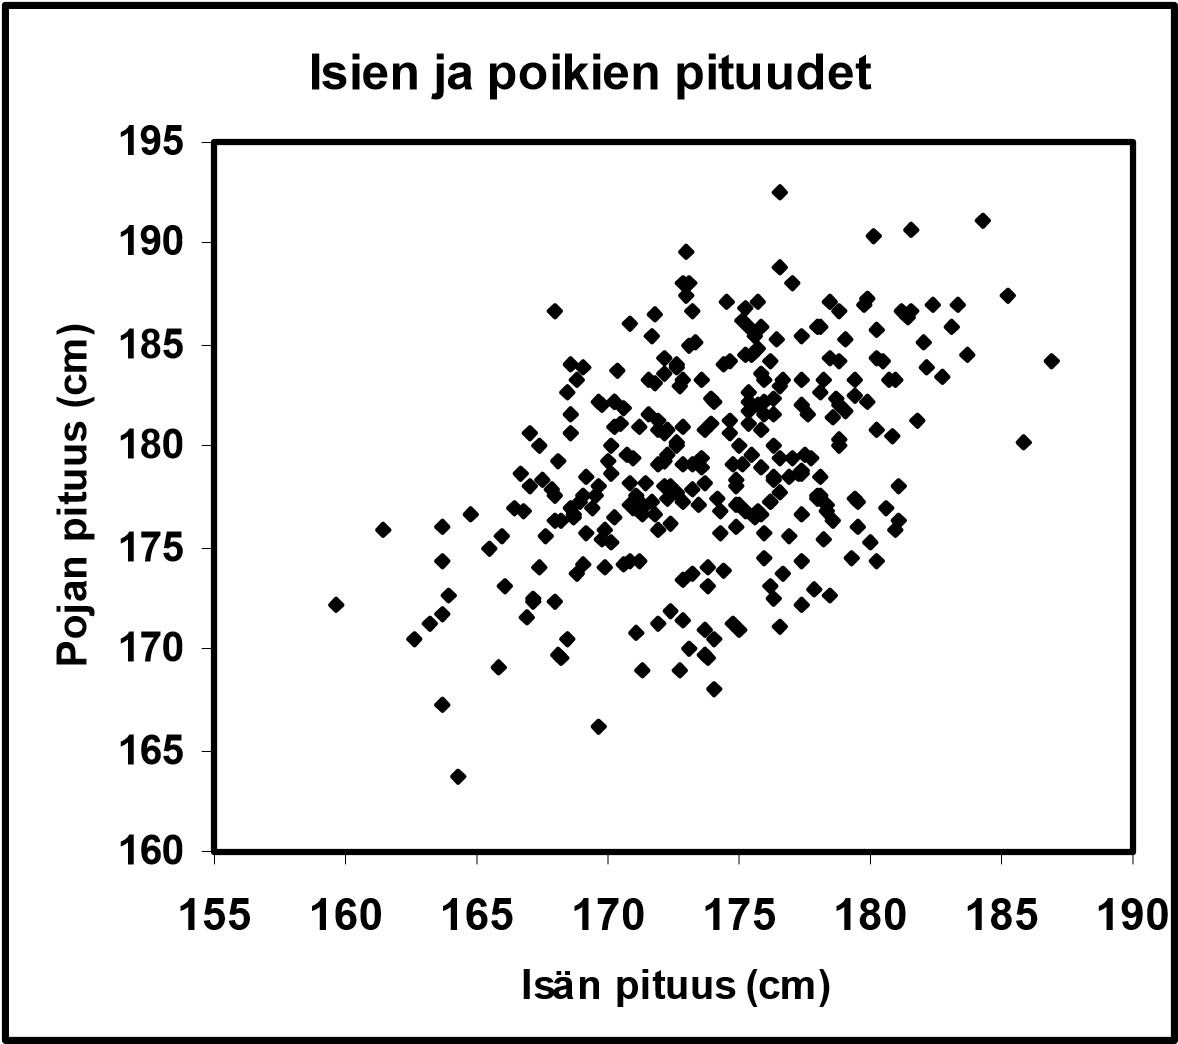
\includegraphics[width=0.75\linewidth]{images/Isien-poikien-pituudet-Mellin} 

}

\caption{Isien ja poikien pituudet. Lähde: Mellin (2006).}\label{fig:isatjapojat1}
\end{figure}

\hypertarget{alaluku73}{%
\section{Tunnusluvut}\label{alaluku73}}

\begin{itemize}
\item
  Kahden välimatka- tai suhdeasteikollisen muuttujan havaintoarvojen parien muodostamaa jakaumaa voidaan karakterisoida seuraavilla tunnusluvuilla:

  \begin{itemize}
  \tightlist
  \item
    Havaintoarvojen keskimääräistä sijaintia kuvataan aritmeettisilla keskiarvoilla.
  \item
    Havaintoarvojen hajaantuneisuutta tai keskittyneisyyttä kuvataan keskihajonnoilla tai (otos-) variansseilla.
  \item
    Havaintoarvojen (lineaarista) riippuvuutta kuvataan otoskovarianssilla ja otoskorrelaatiokertoimella.
  \end{itemize}
\item
  Ts. oletetaan seuraavassa, että meillä on käytettävissä välimatka- tai suhdeasteikollisten muuttujien \(x\) ja \(y\) havaittuja arvoja \(x_1, x_2, \ldots, x_n\) ja \(y_1, y_2, \ldots, y_n\). Oletetaan lisäksi, että havaintoarvot \(x_i\) ja \(y_i\) liittyvät samaan havaintoyksikköön kaikille \(i = 1, 2, \ldots, n\) muodostaen havaintoyksikkökohtaisia havaintoarvojen pareja \((x_i, y_i)\).
\item
  Käsitellään seuraavassa otoskeskiarvoa ja otosvarianssia. Olemme käsitelleet vastaavia estimaattoreita jo aiemmin luvussa \ref{luku6}.
\item
  Havaintoarvojen \(y_1, y_2,\ldots, y_n\) aritmeettinen keskiarvo on
  \[
    \bar{y} = \frac{1}{n} \sum_{i=1}^{n} y_i.
  \]
  Vastaavalla tavalla voidaan määritellä havaintojen \(x_1, x_2, \ldots, x_n\) (aritmeettinen) keskiarvo \(\bar{x}=\frac{1}{n}\sum_{i=1}^{n}x_i\).

  \begin{itemize}
  \tightlist
  \item
    Havaintoarvojen pareista \((x_i, y_i ), \, i = 1, 2,\ldots,n,\) laskettujen aritmeettisten keskiarvojen, otoskeskiarvojen, \(\bar{x}\) ka \(\bar{y}\) muodostama lukupari (\(\bar{x}, \bar{y})\) on havaintoarvojen parien muodostamien pisteiden painopiste.
  \item
    Havaintoarvojen aritmeettinen keskiarvo kuvaa havaintoarvojen keskimääräistä sijaintia.
  \item
    Osoittautuu, että (aritmeettinen) keskiarvo toimii tilastollisessa mielessä hyvänä estimaattorina satunnaismuuttujan \(Y\) odotusarvolle.
  \end{itemize}
\end{itemize}

\hfill\break

\begin{itemize}
\tightlist
\item
  \textbf{Otosvarianssi}: Havaintoarvojen \(y_1, y_2,\ldots, y_n\) (otos-) varianssi (on todettu jo aiemmin) on muotoa
  \[
    s^2_y = \frac{1}{n-1} \sum_{i=1}^{n} (y_i - \bar{y})^2,
  \]
  jossa \(\bar{y}\) on on y-havaintoarvojen aritmeettinen keskiarvo.

  \begin{itemize}
  \tightlist
  \item
    Jälleen vastaavalla tavalla voidaan määritellä x-havaintoarvojen (otos-) varianssi \(S^2_x\).
  \item
    Havaintoarvojen varianssi mittaa havaintoarvojen hajaantuneisuutta tai keskittyneisyyttä havaintoarvojen aritmeettisen keskiarvon suhteen.
  \end{itemize}
\item
  \textbf{(Otos-) keskihajonta}: Havaintoarvojen \(y_1, y_2,\ldots, y_n\) (otos-) keskihajonta
  \[
    s_y = \sqrt{s^2_y} = \sqrt{\frac{1}{n-1} \sum_{i=1}^{n} (y_i - \bar{y})^2},
  \]
  jossa \(\bar{y}\) on on y-havaintoarvojen aritmeettinen keskiarvo. Huomaa suhde otosvarianssiin.

  \begin{itemize}
  \tightlist
  \item
    Jälleen vastaavalla tavalla voidaan määritellä x-havaintoarvojen (otos-) keskihajonta \(s_x\).
  \item
    Havaintoarvojen keskihajonta mittaa havaintoarvojen hajaantuneisuutta tai keskittyneisyyttä havaintoarvojen aritmeettisen keskiarvon suhteen.
  \end{itemize}
\end{itemize}

\hfill\break

\hypertarget{alaluku74}{%
\section{Satunnaismuuttujien kovarianssi ja korrelaatio}\label{alaluku74}}

\begin{itemize}
\item
  Tarkastellaan välimatka- tai suhdeasteikollisten satunnaismuuttujien \(X\) ja \(Y\) (Pearsonin tulomomentti-) korrelaatiokerrointa \(\rho_{XY}\) ja sen estimointia.
\item
  Tällä kurssilla emme tarkastele tarkemmin tilastollisia testejä korrelaatiokertoimelle \(\rho_{XY}\), kuten:

  \begin{itemize}
  \tightlist
  \item
    Yhden otoksen testi korrelaatiokertoimelle
  \item
    Korrelaatiokertoimien vertailutesti
  \item
    Korreloimattomuuden testaaminen
  \end{itemize}
\item
  Jälleen kerran, lisätietoja ja tarkempia yksityiskohtia moniulotteisista satunnaismuuttujista ja jakaumista tarkastellaan todennäköisyyslaskennan kursseilla.
\end{itemize}

\begin{defblock}{}
\textbf{Satunnaismuuttujien kovarianssi ja korrelaatio}

Olkoon \((X, Y)\) satunnaismuuttujien \(X\) ja \(Y\) muodostama järjestetty pari. Olkoot
\[
\mu_X = \text{E}(X) \qquad \mathrm{ja} \qquad  \mu_Y = \text{E}(Y)
\]
satunnaismuuttujien \(X\) ja \(Y\) odotusarvot ja
\begin{align*}
\sigma^2_X &= \mathrm{Var}(X) = \text{D}^2(X) = \text{E}[(X - \mu_X)^2] \\
\sigma^2_Y &= \mathrm{Var}(Y) = \text{D}^2(Y) = \text{E}[(Y - \mu_Y)^2]
\end{align*}

satunnaismuuttujien \(X\) ja \(Y\) varianssit.

\hfill\break

Määritellään satunnaismuuttujien \(X\) ja \(Y\) kovarianssi \(\sigma_{XY}\) kaavalla
\[
\sigma_{XY} = \mathrm{Cov}(X,Y) = \text{E}[(X-\mu_X)(Y-\mu_Y)]
\]

Määritellään satunnaismuuttujien \(X\) ja \(Y\) korrelaatio \(\rho_{XY}\) kaavalla
\[
\rho_{XY} = \mathrm{Cor}(X,Y) = \frac{\sigma_{XY}}{\sigma_{X} \sigma_{Y}},
\]
jossa siis \(\sigma_X = \sqrt{\mathrm{Var}(X)} = \sqrt{\text{D}^2(X)}\) ja \(\sigma_Y = \sqrt{\mathrm{Var}(Y)} = \sqrt{\text{D}^2(Y)}\)

\end{defblock}

\begin{itemize}
\tightlist
\item
  Satunnaismuuttujien \(X\) ja \(Y\) korrelaatiota
  \[
  \rho_{XY} = \mathrm{Cor}(X, Y)
  \]
  kutsutaan ajoittain siis \textbf{Pearsonin korrelaatiokertoimeksi} (tulomomenttikorrelaatiokertoimeksi).

  \begin{itemize}
  \tightlist
  \item
    Pearsonin korrelaatiokerroin \(\rho_{XY}\) mittaa satunnaismuuttujien \(X\) ja \(Y\) lineaarisen riippuvuuden voimakkuutta. Ts. sm:jien välistä (lineaarista) yhteyttä.
  \end{itemize}
\item
  Pearsonin korrelaatiokerrointa voidaan estimoida Pearsonin \textbf{otoskorrelaatiokertoimella}.
\end{itemize}

\begin{defblock}{}
\textbf{Pearsonin otoskorrelaatiokerroin}

Havaintoarvojen \((x_i, y_i)\) pareista laskettu \textbf{otoskovarianssi} on
\[
s_{xy} = \frac{1}{n-1} \sum_{i=1}^{n} (x_i - \bar{x}) (y_i - \bar{y}),
\]
jossa \(\bar{x}\) ja \(\bar{y}\) ovat havaintoarvojen \(x\) ja \(y\) aritmeettiset keskiarvot.\\
Otoskovarianssin \(s_{xy}\) avulla voidaan määritellä \(x\)- ja \(y\)-havaintoarvojen lineaarisen tilastollisen riippuvuuden voimakkuuden mittari, jota kutsutaan Pearsonin otoskorrelaatiokertoimeksi. Pearsonin otoskorrelaatiokerroin \(r_{xy}\) saadaan otoskovarianssista \(s_{xy}\) \textbf{normeerausoperaatiolla}, jossa otoskovarianssi \(s_{xy}\) jaetaan \(x\)- ja \(y\)-havaintoarvojen keskihajonnoilla \(s_x\) ja \(s_y\).\\
Ts. havaintoarvojen pareista \((x_i, y_i), i = 1, 2, \ldots, n,\) laskettu Pearsonin otoskorrelaatiokerroin on siis
\[
r_{xy} = \frac{s_{xy}}{s_x s_y} = \frac{\sum_{i=1}^{n} (x_i - \bar{x}) (y_i - \bar{y})}{\sqrt{\sum_{i=1}^{n} (x_i - \bar{x})^2} \sqrt{\sum_{i=1}^{n} (y_i - \bar{y})^2}} , 
\]
jossa \(s_{xy}\) on \(x\)- ja \(y\)-havaintoarvojen otoskovarianssi, \(s_x\) on \(x\)-havaintoarvojen keskihajonta ja \(s_y\) on \(y\)-havaintoarvojen keskihajonta.

\end{defblock}

\begin{itemize}
\item
  Otoskorrelaatiokertoimen estimaattori voidaan johtaa sekä momenttimenetelmällä että suurimman uskottavuuden menetelmällä, jotka ovat tyypillisiä estimointimenetelmiä tilastotieteessä ja tarkemmin tilastollisessa päättelyssä.
\item
  Otoskovarianssi:

  \begin{itemize}
  \tightlist
  \item
    Huomaa, että \(x\)- ja \(y\)-havaintoarvojen otoskovarianssit niiden itsensä kanssa ovat niiden variansseja.
  \item
    Otoskovarianssi \(s_{xy}\) mittaa \(x\)- ja \(y\)-havaintoarvojen yhteisvaihtelua niiden aritmeettisten keskiarvojen ympärillä.
  \item
    Otoskovarianssilla on taipumus saada positiivisia (negatiivisia) arvoja, jos havaintopisteiden muodostama ``pistepilvi (pisteparvi)'' näyttää nousevalta (laskevalta) oikealle mentäessä; ks. pistediagrammin ilmeen ja Pearsonin otoskorrelaatiokertoimen yhteys, jota käsitellään seuraavaksi.
  \end{itemize}
\item
  Pearsonin otoskorrelaatiokertoimella \(r_{xy}\) on seuraavat ominaisuudet:

  \begin{enumerate}
  \def\labelenumi{\roman{enumi})}
  \tightlist
  \item
    \(-1 \le r_{xy} \le 1\)
  \item
    \(r_{xy} = \pm 1\), jos ja vain jos \(y_i = \alpha \beta x_i\), jossa \(\alpha\) ja \(\beta\) ovat reaalisia vakiota ja \(\alpha,\beta \neq 0\)
  \item
    Korrelaatiokertoimella \(r_{xy}\) ja kovarianssilla \(s_{xy}\) on aina sama etumerkki
  \end{enumerate}
\item
  Pearsonin otoskorrelaatiokerroin \(r_{xy}\): Tulkinta/tulkintoja:

  \begin{itemize}
  \tightlist
  \item
    Havaintoarvojen pareista \((x_i, y_i), i = 1,2, \ldots, n,\) laskettu Pearsonin otoskorrelaatiokerroin \(r_{xy}\) mittaa \(x\)- ja \(y\)-havaintoarvojen lineaarisen tilastollisen riippuvuuden voimakkuutta.
  \item
    Jos \(r_{xy} = \pm 1\), niin \(x\)- ja \(y\)-havaintoarvojen välillä on eksakti eli funktionaalinen lineaarinen riippuvuus, mikä merkitsee sitä, että kaikki havaintopisteet \((x_i, y_i)\) asettuvat samalle suoralle.
  \item
    Jos \(r_{xy} = 0\), niin \(x\)- ja \(y\)-havaintoarvojen välillä ei voi olla eksaktia lineaarista riippuvuutta.
  \item
    Vaikka \(r_{xy} = 0\), \(x\)- ja \(y\)-havaintoarvojen välillä saattaa silti olla jopa eksakti epälineaarinen riippuvuus.
  \end{itemize}
\item
  \textbf{Havainnollistus}: Alapuolella esitettävät kuviot (Kuva \ref{fig:korrelaatioMellin}) havainnollistavat kahden muuttujan havaittujen arvojen (\(n = 30\)) pistediagrammin ilmeen ja korrelaation välistä yhteyttä.
\end{itemize}

\FloatBarrier

\begin{figure}

{\centering 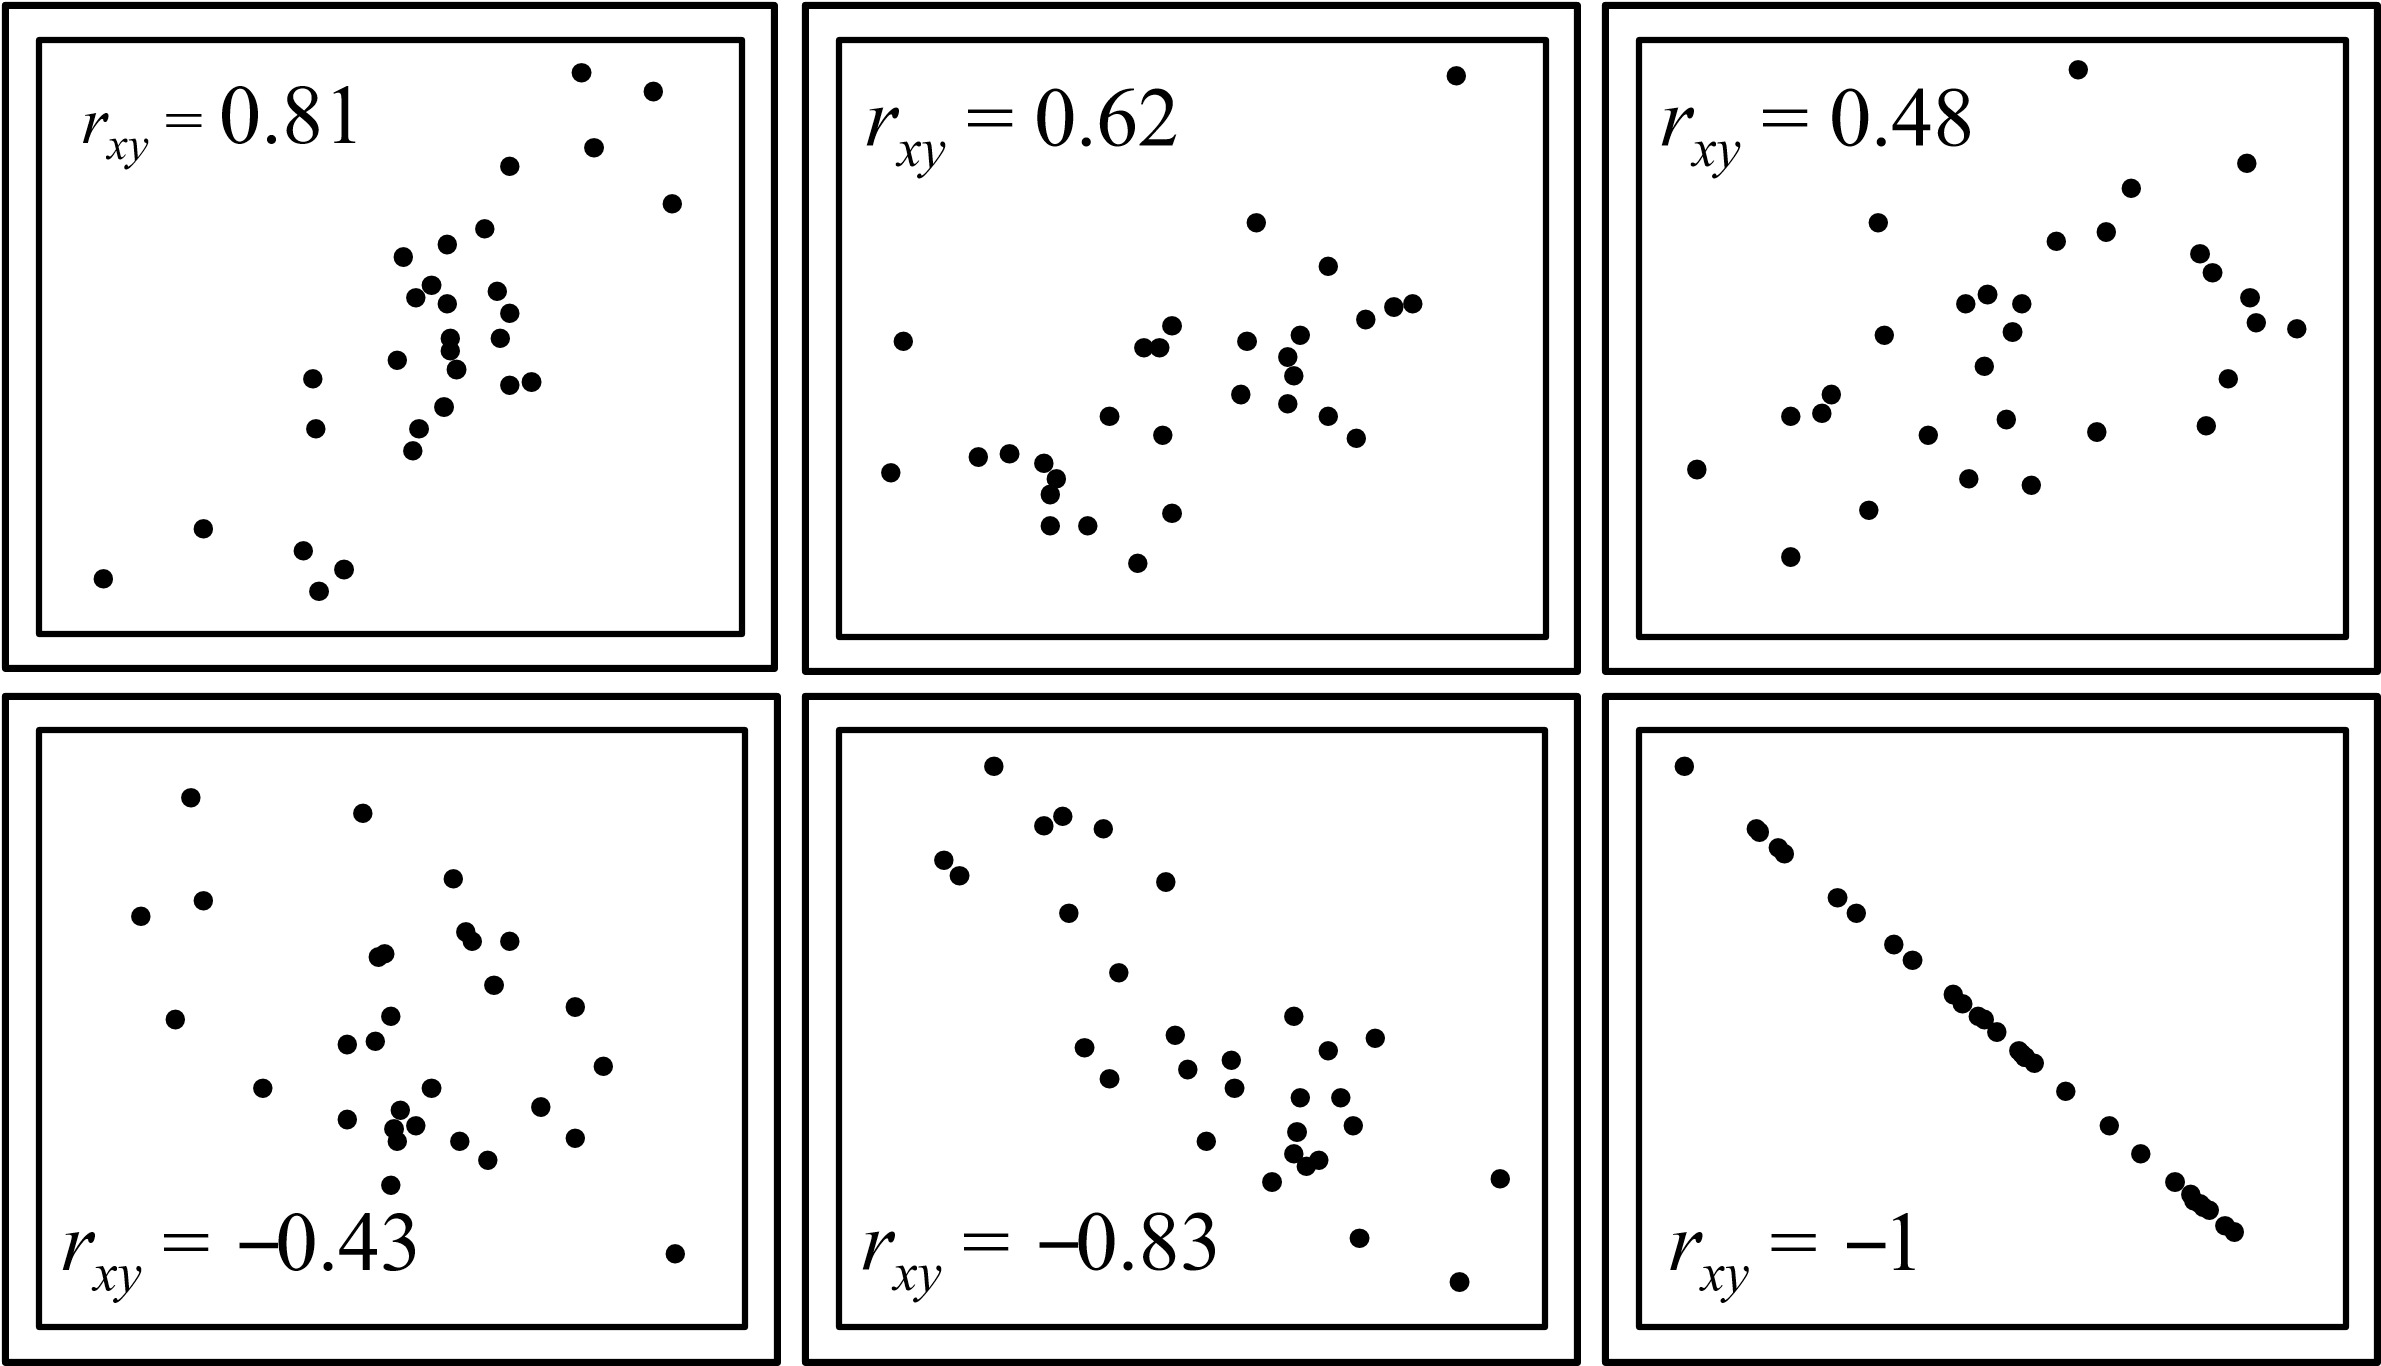
\includegraphics[width=0.9\linewidth]{images/Pearson-korr-Mellin} 

}

\caption{Havainnollistuksia Pearsonin otoskorrelaatiokertoimen arvosta ja erilaisista $xy$-pisteparvista. Lähde: Mellin (2006).}\label{fig:korrelaatioMellin}
\end{figure}

\begin{itemize}
\tightlist
\item
  Ks. seuraavasta \href{http://guessthecorrelation.com/}{linkistä} lisää havainnollistuksia.

  \begin{itemize}
  \tightlist
  \item
    \emph{Guess the correlation} pelissä pääset arvioimaan esitettävän pisteparven korrelaation voimakkuutta erilaisissa simuloiduissa tilanteissa: \url{http://guessthecorrelation.com/}
  \end{itemize}
\end{itemize}

\FloatBarrier

\begin{itemize}
\item
  \textbf{Kausaalisuus}

  \begin{itemize}
  \tightlist
  \item
    Muuttujan \(x\) arvojen muutos vaikuttaa muuttujan \(y\) arvoihin (syy-vaikutussuhde), jos seuraavat kolme ehtoa täyttyvät:

    \begin{itemize}
    \tightlist
    \item
      muuttujan \(x\) muutos esiintyy ajallisesti ennen \(y\):n muutosta.
    \item
      muuttujissa \(x\) ja \(y\) tapahtuvien muutosten välillä on riippuvuutta.
    \item
      muuttujassa \(y\) tapahtunutta muutosta ei voida selittää millään muilla tekjöillä.
    \end{itemize}
  \end{itemize}
\item
  Kausaalisuhteita selvitettäessä on tunnettava etukäteen ilmiötä koskevat aiemmat teoriat ja tutkimukset tarkasti, jotta voidaan ottaa huomioon ilmiöön vaikuttavat tekijät
\item
  Todellisuus on usein monimutkaisempi, kuin mitä kausaalisuhde kuvaa: \textbf{kahden muuttujan yhteisvaihtelu ei riitä todisteeksi siitä, että kyseessä olevien muuttujien välillä on kausaalista yhteyttä}
\item
  Yhteisvaihtelu voi johtua myös kolmannen muuttujan vaikutuksesta molempiin muuttujiin tai virheellisestä otannasta, vaikka muuttujat olisivatkin perusjoukossa toisistaan riippumattomia
\end{itemize}

\FloatBarrier

\begin{figure}

{\centering 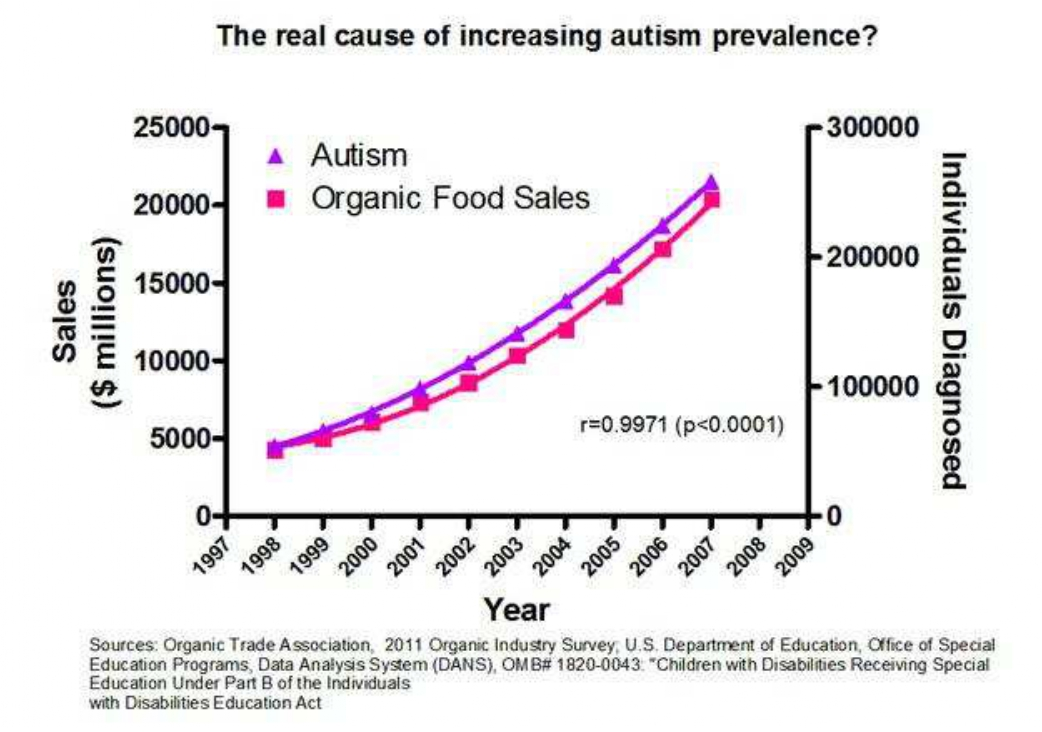
\includegraphics[width=0.75\linewidth]{images/causality2} 

}

\caption{Esimerkkejä: luomuruoka syypää lisääntyneisiin autismitapauksiin?}\label{fig:unnamed-chunk-8}
\end{figure}

\begin{itemize}
\tightlist
\item
  Simpsonin paradoksi

  \begin{itemize}
  \tightlist
  \item
    Simpsonin paradoksi syntyy, kun kahden muuttujan välinen korrelaatio muuttuu päinvastaiseksi, otettaessa huomioon jokin kolmas muuttuja, joka korreloi molempien muuttujien kanssa
  \end{itemize}
\end{itemize}

\FloatBarrier

\begin{figure}

{\centering 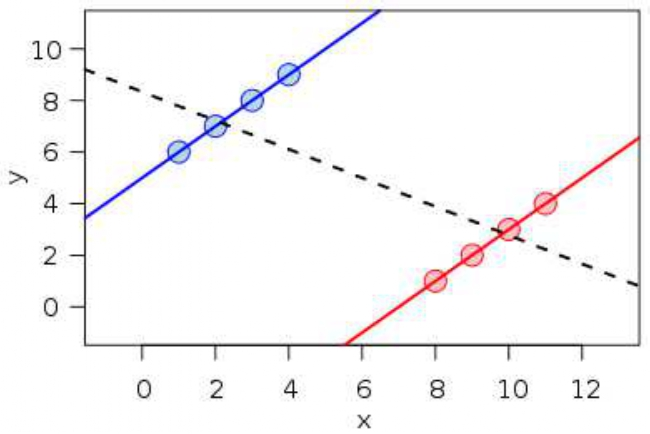
\includegraphics[width=0.75\linewidth]{images/simpson} 

}

\caption{Simpsonin paradoksi}\label{fig:simpson}
\end{figure}

\FloatBarrier

\newpage

\begin{defblock}{}

\textbf{Esimerkki: Berkeleyn sukupuolisyrjintä}

Yksi tunnetuimmista esimerkeistä Simpsonin paradoksista on Berkeleyn yliopiston sukupuolisyrjintätapaus. Yliopisto haastettiin oikeuteen vuonna 1973 sukupuolisyrjinnästä. Väitettiin, että yliopistoon olisi miesten helpompi päästä kuin naisten, sillä yhteensä 8442:sta mieshakijasta 44 \% hyväksyttiin kun samat luvut olivat naisilla 4321 ja 35 \%. Mieshakijoista pääsi siis 9 prosenttiyksikköä enemmän sisälle kuin naisista.

\begin{itemize}
\tightlist
\item
  Tarkasteltaessa erikseen eri tiedekuntia huomataan, että itseasissa useammassa tiedekunnissa naisia on päässyt sisälle isompi osuus hakijoista. Aineisto kuudesta isoimmasta tiedekunnasta on listattu alla olevaan taulukkoon.
\end{itemize}

\end{defblock}

\FloatBarrier

\begin{table}
\centering\begingroup\fontsize{12}{14}\selectfont

\begin{tabular}{lllll}
\toprule
\multicolumn{2}{c}{Miehet} & \multicolumn{3}{c}{Naiset} \\
\cmidrule(l{3pt}r{3pt}){1-2} \cmidrule(l{3pt}r{3pt}){3-5}
Tiedekunta & Hakijat & Hyväksytyt \% & Hakijat & Hyväksytyt \%\\
\midrule
A & 825 & 62 & 108 & 82\\
B & 560 & 63 & 25 & 68\\
C & 325 & 37 & 593 & 34\\
D & 417 & 33 & 375 & 35\\
E & 191 & 28 & 393 & 24\\
\addlinespace
F & 373 & 6 & 341 & 7\\
\bottomrule
\end{tabular}
\endgroup{}
\end{table}

\FloatBarrier

\begin{itemize}
\tightlist
\item
  Vielä tiivistäen korrelaatiokertoimen tulkintavirheitä aiheuttavat useimmiten seuraavat seikat:

  \begin{itemize}
  \tightlist
  \item
    Riippuvuudesta ei välttämättä seuraa syy-seuraussuhdetta.
  \item
    Kolmas muuttuja eli kahden muuttujan välinen yhteys selittyy yhteisestä syystä (esimerkiksi lämpimästä kesästä).
  \item
    Muuttujien välinen yhteys ei ole lineaarinen.
  \item
    Poikkeavien havaintojen vaikutus.
  \end{itemize}
\item
  Puutteita: Korrelaatiokertoimella on kaksi puutetta:

  \begin{itemize}
  \tightlist
  \item
    Se mittaa vain lineaarista riippuvutta.
  \item
    Se ei ole (tilastollinen) malli, jonka avulla nähtäisiin, miten toinen muuttuja vaikuttaa toiseen muuttujaan.
  \end{itemize}
\end{itemize}

\hypertarget{luvun-7-yhteenveto-keskeisiuxe4-termejuxe4-ja-kokonaisuuksia.}{%
\section{Luvun 7 yhteenveto, keskeisiä termejä ja kokonaisuuksia.}\label{luvun-7-yhteenveto-keskeisiuxe4-termejuxe4-ja-kokonaisuuksia.}}

\begin{itemize}
\tightlist
\item
  Eksakti ja tilastollinen riippuvuus
\item
  Korrelaatio
\item
  Kovarianssi
\item
  Pearsoninkin korrelaatiokerroin ja otoskorrelaatiokerroin
\item
  Pistediagrammi
\item
  Kausalisuus vs.~korrelaatio
\end{itemize}

\hypertarget{luku8}{%
\chapter{Regressioanalyysi}\label{luku8}}

Tilastollinen riippuvuus ja korrelaatio -jakson laajennuksena pyrimme tässä luvussa vastaamaan seuraavaan kysymykseen: \emph{Miten jonkin selitettävän muuttujan tilastollista riippuvuutta joistakin toisista, selittäviksi muuttujiksi kutsutuista muuttujista voidaan mallintaa}? Muuttujien välisten riippuvuuksien, eli erilaisten tosielämän asioiden ja ilmiöiden välisten yhteyksien analysointi on tavallisesti keskeinen kysymys tieteellisessä tutkimuksessa. Regressioanalyysi on yksi tunnetuimpia ja eniten sovellettuja \textbf{tilastollisia menetelmiä} kuvaamaan kahden muuttujan \textbf{tilastollista riippuvuutta}.

Jos tilastoaineistossa on havaittavissa säännönmukaisuutta ja muuttujien välillä näyttäisi olevan järkevä (asialooginen) yhteys, niin päästään ``malliajatteluun''. Ts. pyritään rakentamaan tilastollista mallia kys. aineistolle. Pyritään siis muodostaa tilastollinen malli että se valitun kriteeristön perusteella parhaiten kuvaa analysoitavaa pistejoukkoa.

\hypertarget{alaluku81}{%
\section{Johdatus regressioanalyysin ideaan}\label{alaluku81}}

\begin{itemize}
\tightlist
\item
  Regressioanalyysi pyrkii siis havaintoaineiston perusteella \textbf{mallintamaan tilastoyksikköjen tilastollisten muuttujien välistä riippuvuutta}.

  \begin{itemize}
  \tightlist
  \item
    Regressiomallissa tilastollisia muuttujia on kahdenlaisia: \textbf{selitettävä muuttuja}, jonka tilastollista vaihtelua pyritään selittämään \textbf{selittävän muuttujan}, tai \textbf{selittävien muuttujien}, vaihtelulla.
  \item
    Toisin sanoen, pyritään erottamaan se selitettävän muuttujan arvojen vaihtelu, joka voidaan selittää selittävän muuttujan arvojen vaihtelulla siitä vaihtelusta, joka on täysin satunnaista.

    \begin{itemize}
    \tightlist
    \item
      Esimerkiksi voitaisiin tutkia selittääkö vaaleissa puolueiden/ehdokkaiden vaalimainontabudjetti heidän äänimääriään, ja jos selittää, niin kuinka paljon?
    \item
      Jos \textbf{tilastollisesti merkitsevä osa} selitettävän muuttujan havaittujen arvojen vaihtelusta voidaan selittää selittävien muuttujien arvojen vaihtelun avulla, sanomme, että selitettävä muuttuja \textbf{riippuu tilastollisesti} selittäjinä käytetyistä muuttujista.
    \end{itemize}
  \end{itemize}
\item
  Yleisemmin regressioanalyysi pyrkii vastaamaan seuraaviin kysymyksiin koskien tilastollisten muuttujien välistä riippuvuutta:

  \begin{itemize}
  \tightlist
  \item
    Muuttujien välisten \textbf{riippuvuuksien kuvaaminen}. Millainen on riippuvuuden muoto? Kuinka voimakasta riippuvuus on?
  \item
    Muuttujien välisten \textbf{riippuvuuksien selittäminen}. Tilastollisen riippuvuuden luonteen selittäminen.
  \item
    Selitettävän muuttujan käyttäytymisen \textbf{ennustaminen}.
  \end{itemize}
\item
  \textbf{Lineaarinen regressioanalyysi} siis (teknisesti) rajoittuu muuttujien \emph{lineaaristen} riippuvuuksien kuvaamiseen. Kuitenkin, laajemmin asiaa pohdittaessa, lineaaristen regressiomallien suuri käyttökelpoisuus muuttujien välisten riippuvuuksien tilastollisessa analyysissa perustuu (ainakin) seuraaviin seikkoihin:

  \begin{itemize}
  \tightlist
  \item
    Lineaarisella regressiomallilla voidaan usein vähintään kohtuullisella (riittävällä) tarkkuudella approksimoida epälineaarisiakin muuttujien välisiä riippuvuuksia!
  \item
    Muuttujien välinen epälineaarinen riippuvuus voidaan usein myös linearisoida käyttäen sopivia muunnoksia alkuperäisiin muuttujiin.
  \item
    Epälineaariset regressiomallit muodostavat oman tilastollisten (regressio)mallien luokkansa (joita ei käsitellä tällä kurssilla, mutta kylläkin myöhemmissä tilastotieteen opinnoissa).
  \end{itemize}
\item
  Regressiomalleja käytetään apuvälineinä monilla tilastotieteen osa-alueilla. Esimerkkejä regressiomallien käyttökohteista tilastotieteessä:

  \begin{itemize}
  \tightlist
  \item
    Varianssianalyysi
  \item
    Koesuunnittelu
  \item
    Monimuuttujamenetelmät
  \item
    Biometria/biostatistiikka
  \item
    Aikasarja-analyysi ja ennustaminen
  \item
    Ekonometria
  \end{itemize}
\item
  Regressioanalyysissa sovellettavat tilastolliset mallit voidaan luokitella usealla eri periaatteella.

  \begin{itemize}
  \tightlist
  \item
    Luokittelu regressiomallin funktionaalisen muodon mukaan:

    \begin{itemize}
    \tightlist
    \item
      Lineaariset regressiomallit
    \item
      Epälineaariset regressiomallit
    \end{itemize}
  \item
    Luokittelu regressiomallin yhtälöiden lukumäärän mukaan:

    \begin{itemize}
    \tightlist
    \item
      Yhden yhtälön regressiomallit
    \item
      Moniyhtälömallit
    \end{itemize}
  \end{itemize}
\end{itemize}

Tällä kurssilla käsitellään vain \textbf{lineaarisia yhden yhtälön regressiomalleja}. Kuitenkin luvussa \ref{alaluku83} esitellään lyhyesti minkälaisia laajennuksia tälle regressioanalyysin perustilanteelle tyypillisesti käsitellään.

\hypertarget{alaluku82}{%
\section{Yhden selittäjän lineaarinen regressiomalli}\label{alaluku82}}

\begin{itemize}
\item
  Yhden selittäjän lineaarinen regressiomalli pyrkii selittämään selitettävän muuttujan havaittujen arvojen vaihtelun yhden selittävän muuttujan havaittujen arvojen vaihtelun avulla. Se on siis yksinkertaisin esimerkki yhden yhtälön lineaarisista regressiomalleista, sillä se sisältää vain yhden selittävän muuttujan useamman sijaan.

  \begin{itemize}
  \tightlist
  \item
    Selitettävää muuttujaa kutsutaan usein myös \emph{vastemuuttujaksi, riippuvaksi muuttujaksi tai tulosmuuttujaksi}
  \item
    Vastaavasti selittävää muuttujaa kutsutaan paikoin \emph{selittäjäksi, riippumattomaksi muuttujaksi tai ennustavaksi muuttujaksi}.
  \end{itemize}
\item
  Tässä luvussa tarkastellaan lyhyesti ja tiivistetysti seuraavia yhden selittävän muuttujan lineaarisen regressiomallin soveltamiseen liittyviä kysymyksiä:

  \begin{itemize}
  \tightlist
  \item
    Miten malli formuloidaan?
  \item
    Mitkä ovat mallin osat ja mitkä ovat osien tulkinnat?
  \item
    Mitkä ovat mallia koskevat oletukset?
  \item
    Miten mallin parametrit estimoidaan?
  \item
    Miten mallin parametreja koskevia hypoteeseja testataan?
  \item
    Miten mallin hyvyyttä mitataan?
  \item
    Miten mallilla ennustetaan?
  \end{itemize}
\item
  Oletetaan, että selitettävän muuttujan \(Y\) havaittujen arvojen vaihtelua halutaan selittää selittävän muuttujan eli selittäjän \(x\) havaittujen arvojen vaihtelun avulla. Tulkitaan selittävä muuttuja tässä kohtaa kiinteäksi eli sen arvot oletetaan tunnetuksi.\footnote{Kyseinen muuttuja voidaan myös tulkita satunnaismuuttujana eikä seuraavat tarkastelut muutu ratkaisevasti tämän seurauksena. Tätä pohditaan vielä tarkemmin alempana.}
\item
  Tehdään siis seuraavat oletukset:

  \begin{enumerate}
  \def\labelenumi{\roman{enumi})}
  \tightlist
  \item
    Selitettävä muuttuja Y on suhdeasteikollinen satunnaismuuttuja.
  \item
    Selittävä muuttuja x on kiinteä eli ei-satunnainen muuttuja.
  \end{enumerate}
\item
  Olkoot \(y_1, y_2,\ldots, y_n\) selitettävän muuttujan \(Y\) ja \(x_1, x_2, \ldots, x_n\) selittävän muuttujan \(x\) havaittuja arvoja. Oletetaan lisäksi, että havaintoarvot \(x_i\) ja \(y_i\) liittyvät
  samaan havaintoyksikköön kaikille \(i=1, 2, \ldots, n\).

  \begin{itemize}
  \tightlist
  \item
    Matemaattisemmin tämä tarkoittaa sitä, että tällöin havaintoarvot muodostavat pisteitä 2-ulotteisessa \((x_i, Y_i)\) avaruudessa.
  \end{itemize}
\item
  Oletetaan seuraavaksi, että havaintoarvojen \(y_i\) ja \(x_i\) välillä on \textbf{lineaarinen tilastollinen riippuvuus}, joka voidaan ilmaista yhtälöllä
  \[
  Y_i = \beta_0 + \beta_1 x_i + \varepsilon_i, \quad i=1,\ldots, n.
  \]
\item
  Tämä yhtälö määrittelee yhden selittäjän lineaarisen regressiomallin, jossa

  \begin{itemize}
  \tightlist
  \item
    \(y_i\) on selitettävän muuttujan \(Y\) satunnainen ja havaittu arvo havaintoyksikölle \(i\).
  \item
    \(x_i\) selittävän muuttujan eli selittäjän \(x\) ei-satunnainen ja havaittu arvo havaintoyksikölle \(i\).
  \item
    \(\varepsilon_i\) on virhetermi (ajoittain myös jäännöstermi) ja sen satunnainen ja ei-havaittu arvo havaintoyksikölle \(i\).
  \end{itemize}
\item
  Yhden selittäjän lineaarisessa regressiomallissa on seuraavat regressiokertoimet:

  \begin{itemize}
  \tightlist
  \item
    \(\beta_0\) on vakioselittäjän regressiokerroin; \(\beta_0\) on ei-satunnainen ja tuntematon vakio. Kerrointa \(\beta_0\) kutsutaan myös vakioselittäjän regressiokertoimeksi. Nimitys johtuu siitä, että kerrointa \(\beta_0\) vastaa keinotekoinen selittäjä, joka saa kaikille havaintoyksiköille \(i=1, 2, \ldots, n\) vakioarvon 1.

    \begin{itemize}
    \tightlist
    \item
      Huomautus: Jatkossa esitettävät kaavat eivät välttämättä päde esitettävässä muodossa, jos mallissa ei ole vakiota (vakioselittäjää), joka yleensä automaattisesti lisätään mukaan malliin.
    \item
      Oletamme jatkossa, että mallissa on aina vakioselittäjä.
    \end{itemize}
  \item
    \(\beta_1\) on selittäjän \(x\) regressiokerroin; \(\beta_1\) on ei-satunnainen ja tuntematon vakio

    \begin{itemize}
    \tightlist
    \item
      Huomautus: Regressiokertoimet \(\beta_0\) ja \(\beta_1\) on oletettu samoiksi kaikille havaintoyksiköille \(i\).
    \end{itemize}
  \end{itemize}
\item
  Virhetermeistä \(\varepsilon_i\) tehtävät ns. standardioletukset ovat seuraavat:

  \begin{enumerate}
  \def\labelenumi{\roman{enumi})}
  \tightlist
  \item
    \(\text{E}(\varepsilon_i) = 0, \, i=1,2,\ldots,n\).
  \item
    Virhetermeillä on vakiovarianssi eli ne ovat homoskedastisia: \(\mathrm{Var}(\varepsilon_i)= \sigma^2, \, i=1,\ldots,n\). Virhetermien \(\varepsilon_i\) tässä yhteiseksi oletettua varianssia kutsutaan ajoittain jäännösvarianssiksi.
  \item
    Virhetermit ovat korreloimattomia: \(\mathrm{Cov}(\varepsilon_i, \varepsilon_l)=0, \, i \neq l\).
  \item
    Lisäksi tehdään ajoittain normaalisuusoletus eli että virhetermit ovat normaalisti jakautuneita: \(\varepsilon_i \thicksim \text{N}(0, \sigma^2), \, i=1,2,\ldots,n\).
  \end{enumerate}

  \begin{itemize}
  \tightlist
  \item
    Huomautus: Oletus (iv) sisältää oletukset (i) ja (ii).
  \end{itemize}
\item
  Lineaarisen regressiomallin perusoletuksiin kuuluu se, että selittävien muuttujien arvot ovat ei-satunnaisia. On kuitenkin syytä korostaa (jo tässä vaiheessa), että selittävän muuttujan arvojen satunnaisuus ei kuitenkaan vaikuta mallin estimoinnissa ja testauksessa käytettäviin menetelmiin seuraavissa tilanteissa:

  \begin{itemize}
  \tightlist
  \item
    Tavanomaiset mallista tehdyt oletukset pätevät (sopivasti modifioituina), kun siirrytään tarkastelemaan selittävän muuttujan ehdollista odotusarvoa selittäjien suhteen.
  \item
    Voidaan (ajoittain) olettaa, että selitettävä muuttuja ja selittäjät noudattavat yhdessä \textbf{multinormaalijakaumaa} eli aiemmin esitellyn yksiulotteisen normaalijakauman moniulotteista laajennusta.
  \end{itemize}
\end{itemize}

\hfill\break

\begin{itemize}
\tightlist
\item
  Regressioanalyysille voidaan esittää kaksi asialoogisesti varsin erilaista lähtökohtaa, joilla on kuitenkin myös monia yhtymäkohtia:

  \begin{enumerate}
  \def\labelenumi{\roman{enumi})}
  \tightlist
  \item
    Ongelmat determinististen mallien sovittamisessa havaintoihin: Havainnoille esitetty malli ei sovi täsmällisesti kaikkiin havaintoihin. Tämä onkin osaltaan tilastollisen mallinnuksen yksi ominaispiirteistä: Täydellistä sopivuutta aineiston kanssa ei käytännössä koskaan saavuteta.
  \item
    Tavoitteena on moniulotteisen todennäköisyysjakauman regressiofunktion parametrien estimointi.
  \end{enumerate}

  \begin{itemize}
  \tightlist
  \item
    Vaikka moniulotteisten todennäköisyysjakaumien regressiofunktiot ovat yleisesti epälineaarisia, lineaariset regressiomallit muodostavat tärkeän ja paljon sovelletun malliluokan.
  \end{itemize}
\item
  Koska regressiokertoimet \(\beta_0\) ja \(\beta_1\) sekä jäännösvarianssi \(\sigma^2\) ovat tavallisesti tuntemattomia, niiden arvot on \textbf{estimoitava} muuttujien \(x\) ja \(Y\) havaittuja arvoja \(x_i\) ja \(y_i\), \(i=1,2, \ldots, n\) käyttäen.

  \begin{itemize}
  \tightlist
  \item
    Regressiomallien parametrien estimointiin käytetään tavallisesti \textbf{pienimmän neliösumman (PNS) menetelmää}. Tämän estimointimenetelmän tarkemmat yksityiskohdat ovat myöhempien tilastotieteen kurssien asioita, mutta seuraavassa kuitenkin muutamia lähtökohtia mihin PNS-menetelmä perustuu yhden selittäjän mallin tapauksessa.
  \item
    Edellä esitellyn yhden selittäjän lineaarisen regressiomallin regressiokertoimien \(\beta_0\) ja \(\beta_1\) estimaattorit määrätään minimoimalla virhetermien \(\varepsilon_i\) neliösummaa
  \end{itemize}
\end{itemize}

\[
S(\beta_0,\beta_1) = \sum_{i=1}^{n} \varepsilon^2_i = \sum_{i=1}^{n} (y_i - \beta_0 - \beta_1 x_i)^2 
\]
regressiokertoimien \(\beta_0\) ja \(\beta_1\) suhteen.

\begin{itemize}
\item
  Tämä minimointi tapahtuu tavanomaiseen tapaan derivoimalla funktio \(S(\beta_0,\beta_1)\) kertoimien \(\beta_0\) ja \(\beta_1\) suhteen ja merkitsemällä derivaatat nolliksi:
  \begin{align*}
  \frac{\partial S(\beta_0,\beta_1)}{\partial \beta_0} &= -2 \sum_{i=1}^{n} (y_i - \beta_0 - \beta_1 x_i) = 0 \\
  \frac{\partial S(\beta_0,\beta_1)}{\partial \beta_1} &= -2 \sum_{i=1}^{n} (y_i - \beta_0 - \beta_1 x_i) x_i = 0. 
  \end{align*}
\item
  Nämä ns. \textbf{normaaliyhtälöt} johtavat lopulta pienen sieventämisen jälkeen regressiokertoimien \(\beta_0\) ja \(\beta_1\) pienimmän neliösumman (PNS-) estimaattoreihin (ja lopulta käytännössä analysoitavasta aineistosta laskettaviin PNS-estimaatteihin)
  \begin{align*}
  \widehat{\beta}_0 &= \bar{y} - \widehat{\beta}_1 \bar{x} \\
  \widehat{\beta}_1 &= \frac{s_{xy}}{s^2_x} = r_{xy} \frac{s_y}{s_x}.
  \end{align*}
\item
  Huomaa siis yhteys aiemmin keskusteltuihin \(x\):n ja \(y\):n otoskeskiarvioihin, keskihajontoihin sekä otoskovarianssiin ja korrelaatioon \(x\):n ja \(y\):n välillä.
\item
  PNS-estimaattorit (estimaatit) \(\widehat{\beta}_0\) ja \(\widehat{\beta}_1\) määrittelevät suoran (matemaattisesti katsoen avaruudessa \(\mathbb{R}^2\)):
  \[
  \widehat{y} = \widehat{\beta}_0 + \widehat{\beta}_1 x,
  \]
  jossa

  \begin{itemize}
  \tightlist
  \item
    \(\widehat{\beta}_0\) on estimoidun regressiosuoran ja pistekuvion y-akselin leikkauspiste
  \item
    \(\widehat{\beta}_1\) on estimoidun regressiosuoran kulmakerroin
  \end{itemize}
\item
  Tämän suoran tuottamat arvot \(\widehat{y}_i\) ovat käytännössä eri havainnoille \(y\) saatavat \textbf{sovitteet} lineaariseen malliin perustuen.
\end{itemize}

\hfill\break

\begin{itemize}
\item
  Sijoitetaan regressiokertoimien \(\beta_0\) ja \(\beta_1\) PNS-estimaattoreiden lausekkeet estimoidun regressiosuoran lausekkeeseen. Tällöin estimoidun regressiosuoran yhtälö voidaan kirjoittaa muodossa:
  \[
  y = \bar{y} + r_{xy} \frac{s_y}{s_x} (x-\bar{x})
  \]

  \begin{itemize}
  \tightlist
  \item
    Yhtälöstä nähdään, että estimoitu regressiosuora kulkee havaintopisteiden \((x_i , y_i), i = 1,2, \ldots, n,\) painopisteen kautta. Voidaan siis nähdä, että estimoidulla regressiosuoralla on seuraavat ominaisuudet:

    \begin{itemize}
    \item
      \begin{enumerate}
      \def\labelenumi{(\roman{enumi})}
      \tightlist
      \item
        Jos \(r_{xy} > 0\), suora on nouseva.
      \end{enumerate}
    \item
      \begin{enumerate}
      \def\labelenumi{(\roman{enumi})}
      \setcounter{enumi}{1}
      \tightlist
      \item
        Jos \(r_{xy} < 0\), suora on laskeva.
      \end{enumerate}
    \item
      \begin{enumerate}
      \def\labelenumi{(\roman{enumi})}
      \setcounter{enumi}{2}
      \tightlist
      \item
        Jos \(r_{xy} = 0\), suora on vaakasuorassa.
      \end{enumerate}
    \item
      \begin{enumerate}
      \def\labelenumi{(\roman{enumi})}
      \setcounter{enumi}{3}
      \tightlist
      \item
        Suora jyrkkenee (loivenee), jos
      \end{enumerate}

      \begin{itemize}
      \tightlist
      \item
        korrelaation itseisarvo \(|r_{xy}|\) kasvaa (pienenee)
      \item
        keskihajonta \(s_y\) kasvaa (pienenee)
      \item
        keskihajonta \(s_x\) pienenee (kasvaa)
      \end{itemize}
    \end{itemize}
  \end{itemize}
\end{itemize}

\hfill\break

\begin{itemize}
\tightlist
\item
  Tarkastellaan vielä estimoituun lineaariseen malliin liittyviä sovitteita ja residuaaleja.

  \begin{itemize}
  \tightlist
  \item
    Estimoidun mallin \textbf{sovitteet} saadaan siis kaavalla
  \end{itemize}
\end{itemize}

\[
\widehat{y}_i = \widehat{\beta}_0 + \widehat{\beta}_1 x_i, \quad i=1,2,\ldots,n.
\]

\begin{itemize}
\tightlist
\item
  Vastaavasti \textbf{residuaalit} saadaan havaintojen ja sovitteiden erotuksena
\end{itemize}

\[
\widehat{\varepsilon}_i = y_i - \widehat{y}_i = y_i - \widehat{\beta}_0 - \widehat{\beta}_1 x_i, \quad i=1,2,\ldots,n.
\]

\begin{itemize}
\tightlist
\item
  Sovite on estimoidun regressiosuoran yhtälön selitettävälle muuttujalle antama arvo havaintopisteessä \(x_i\). Vastaaavasti residuaali on selitettävän muuttujan havaitun arvon \(y_i\) ja sovitteen \(\widehat{y}_i\) eli estimoidun regressiosuoran yhtälön selitettävälle muuttujalle havaintopisteessä \(x_i\) antaman arvon erotus.

  \begin{itemize}
  \tightlist
  \item
    Estimoitu regressiomalli selittää selitettävän muuttujan havaittujen arvojen vaihtelua sitä paremmin mitä lähempänä estimoidun mallin sovitteet \(\widehat{y}_i\) ovat selitettävän muuttujan havaittuja arvoja \(y_i\).
  \item
    Yhtäpitävästi edellisen kanssa: Estimoitu regressiomalli selittää selitettävän muuttujan havaittujen arvojen \(y_i\) vaihtelua sitä paremmin mitä pienempiä ovat estimoidun mallin residuaalit \(\widehat{\varepsilon}_i\).
  \end{itemize}
\end{itemize}

\hfill\break

\begin{itemize}
\tightlist
\item
  Liittyen vielä estimoidun mallin sopivuuden tarkasteluun, estimoidun regressiomallin hyvyyttä mitataan (tavanomaisesti) mm. \textbf{selitysasteella} (\(R^2)\).

  \begin{itemize}
  \tightlist
  \item
    Selitysasteen määritelmä perustuu ns. varianssianalyysihajotelmaan, jossa selitettävän muuttujan havaittujen arvojen vaihtelua kuvaava neliösumma on jaettu kahdeksi neliösummaksi, joista toinen kuvaa mallin ja havaintojen yhteensopivuutta ja toinen mallin ja havaintojen yhteensopimattomuutta.
  \item
    Selitysaste saa arvoja nollan ja ykkösen väliltä (kun lineaarisessa regressiomallissa on mukana vakiotermi). Arvo 0 tarkoittaa, että malli (yhden selittäjän mallissa käytännössä siis selittäjä \(x\)) ei selitä \(y\):n lineaarista vaihtelua yhtään (yli vakiotermin). Ts. määritelty malli ei ollenkaan selitä selitettävän muuttujan havaittujen arvojen vaihtelua.
  \item
    Vastaavasti arvo \(R^2 = 1\) tarkoittaa, että malli sopii täydellisesti aineistoon. Ts. selitysaste mittaa regressiomallin selittämää osuutta selitettävän muuttujan havaittujen arvojen kokonaisvaihtelusta.
  \item
    Korkea selitysasteen arvo on siis sinänsä usein toivottava lopputulos lineaarisen mallin käytön yhteydessä. Tämän liian mekaaninen tavoittelu johtaa kuitenkin ajoittain muihin ongelmiin, kuten \textbf{ylisovittamiseen} usean selittäjän lineaarisia malleja käsiteltäessä.
  \end{itemize}
\end{itemize}

\hfill\break

\begin{eblock}{}
\textbf{Esimerkki: isän ja poikien pituus, tarkemmin}

Jatketaan isän ja heidän poikiensa pituutta koskevan aineiston tarkastelua. Periytyykö isän pituus heidän pojilleen? Käytännössä jo aiemmin tarkastelimme 300 havainnon havaintoaineistoa isän ja heidän poikiensa pituuksien muodostamista lukupareista.

Estimoidun regressiosuoran yhtälö on (ks. oheinen kuva \ref{fig:isatjapojat2})
\[
y = 97.391+ 0.4707 x
\]
Suoran kulmakertoimen \(\widehat{\beta}_1\) = 0.4707 tulkinta on siis, että jos isä A on 1 cm pitempi kuin isä B, isä A:n poika on keskimäärin 0.4707 cm pitempi kuin isä B:n poika.

\end{eblock}

\begin{figure}

{\centering 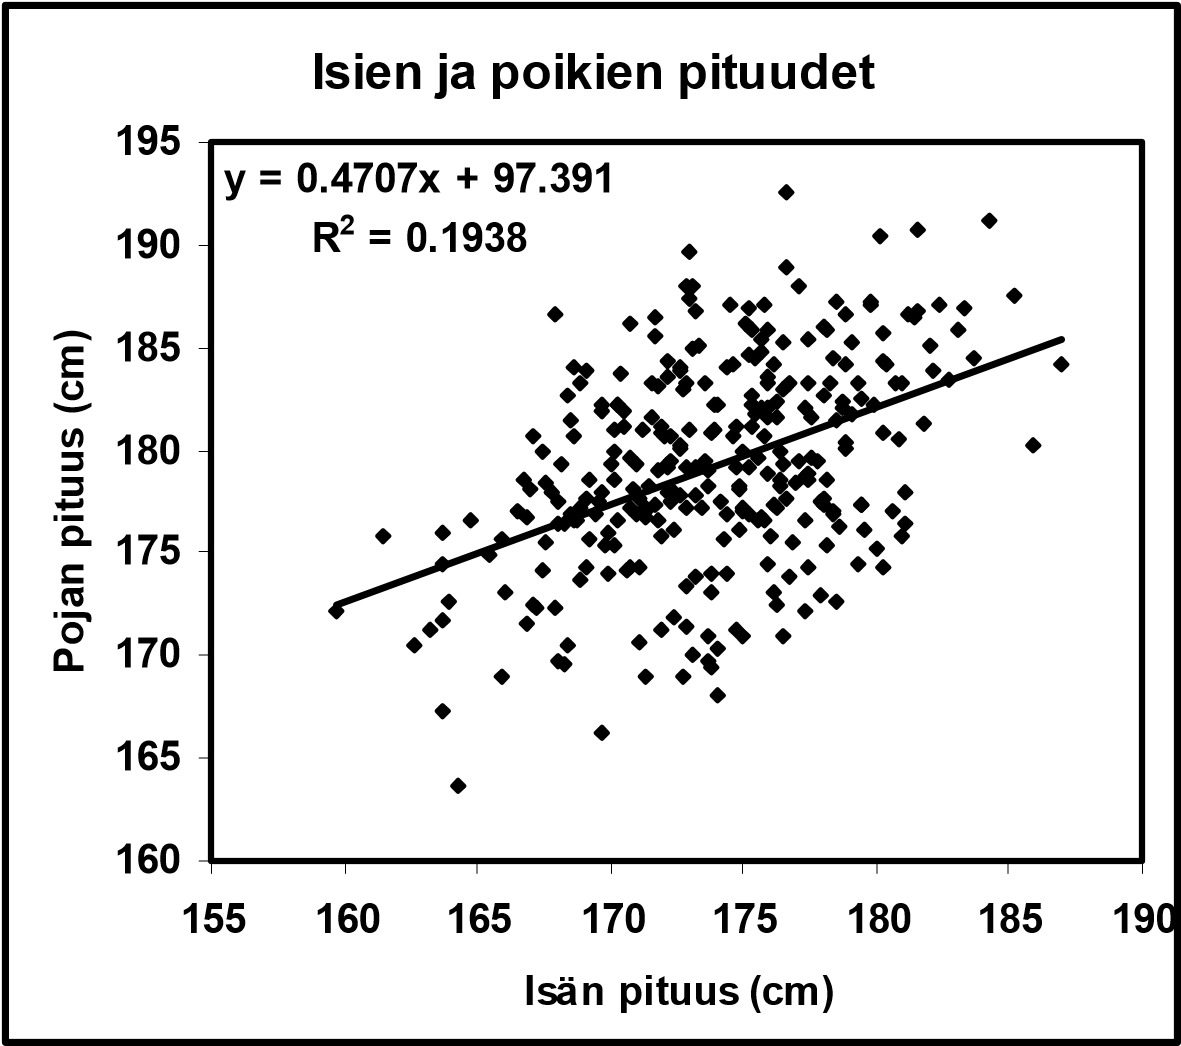
\includegraphics[width=1\linewidth]{images/Sovite-isien-poikien-pituudet-Mellin} 

}

\caption{Isien ja poikien pituudet: regressiosuoran sovite}\label{fig:isatjapojat2}
\end{figure}

\hfill\break

\hypertarget{alaluku83}{%
\section{Muita regressiomalleja}\label{alaluku83}}

\begin{itemize}
\item
  Yksinkertaista lineaarista regressiomallia voidaan laajentaa monin tavoin monenlaisiin erilaisiin tilanteisiin.

  \begin{itemize}
  \tightlist
  \item
    Usean selittäjän lineaarinen regressiomalli: Yhden selittäjän sijaan käytetään useita selittäviä muuttujia.
  \item
    Lineaarisen mallin sijaan malli voi olla myös epälineaarinen (epälineaarinen regressiofunktio).
  \end{itemize}
\item
  Erityisen tärkeitä laajennuksia ilmenee kun \textbf{vastemuuttuja on muuta muotoa} mitä edellä oletetaan lineaarisissa regressiomalleissa, joissa käytännössä oletetaan että vaste on reaaliarvoinen (jokin reaaliluku).

  \begin{itemize}
  \tightlist
  \item
    Vaste voi olla myös \textbf{diskreettiarvoinen}, kuten \textbf{binäärinen} (\(Y_i=0\) tai \(Y_i=1\)) tai \textbf{lukumäärä} \(Y_i \in \{0,1,2,3,\ldots\}\)
  \item
    Mikäli vaste on binäärinen, niin tällöin tyypillinen tarkasteltava ja täsmennettävä tilastollinen malli on \textbf{logistinen regressiomalli} (tunnetaan myös \textbf{logistisena regressiomallina} tai \textbf{logit-mallina}).
  \item
    Jos vaste on lukumäärä, niin tällöin yksi mahdollinen malliluokka on ns. \textbf{Poisson-regressiomalli}. Tässä yhteydessä oletetaan siis, että sm. \(Y\) noudattaa Poisson-jakaumaa ja regressiomalli rakennetaan tämän oletuksen ympärille.
  \end{itemize}
\item
  \textbf{Vastemuuttujan roolin/luonteen selvittäminen on hyvin keskeistä tilastollista mallia rakennettaessa}. Tässä pätee samat eroavaisuudet mitkä tulevat tutuiksi todennäköisyyslaskennan kursseilla kun käsitellään diskreettien ja jatkuva-arvoisten satunnaismuuttujien jakaumia ja näihin liittyviä yksityiskohtia.
\item
  Pitemmälle meneviä regressioanalyysin kysymyksiä käsitellään useilla myöhemmillä tilastotieteen kursseilla.

  \begin{itemize}
  \tightlist
  \item
    Erityisesti aineopintojen kurssien \href{https://opas.peppi.utu.fi/fi/opintojakso/TILM3561/5069}{TILM3561 Tilastollinen päättely I} ja \href{https://opas.peppi.utu.fi/fi/opintojakso/TILM3562/5070}{TILM3562 Tilastollinen päättely II} jälkeisellä \href{https://opas.peppi.utu.fi/fi/opintojakso/TILM3588/5071}{TILM3588 Lineaariset ja yleistetyt lineaariset mallit -kurssilla}, jossa tarvitaan myös lineaarialgebran ja matriisilaskennan tietoja, joita tilastotieteen yhteydessä käydään läpi \href{https://opas.peppi.utu.fi/fi/opintojakso/TILM3574/5082}{TILM3574 Matriisilaskenta tilastotieteessä -kurssilla}.
  \item
    Tämän jälkeen regressiomallien käsittely jatkuu useilla eri aineopintojen ja syventävien opintojen erikoiskursseilla.
  \end{itemize}
\end{itemize}

\hypertarget{luvun-8-yhteenveto-keskeisiuxe4-termejuxe4-ja-kokonaisuuksia.}{%
\section{Luvun 8 yhteenveto, keskeisiä termejä ja kokonaisuuksia.}\label{luvun-8-yhteenveto-keskeisiuxe4-termejuxe4-ja-kokonaisuuksia.}}

\begin{itemize}
\tightlist
\item
  Lineaarinen regressioanalyysi
\item
  Yhden selittäjän lineaarinen regressiomalli
\item
  Selitettävä muuttuja
\item
  Selittävä muuttuja/selittävät muuttujat
\item
  Virhetermi
\item
  Pienimmän neliösumman (PNS) menetelmä
\item
  PNS-estimaattorit ja PNS-estimaatit
\item
  Sovitteet ja residuaalit
\item
  Selitysaste
\end{itemize}

\hypertarget{luku9}{%
\chapter{Tilastotieteen rooli uuden tiedon tuottamisessa}\label{luku9}}

Tilastotieteen yhteiskunnallisesta roolista keskusteltiin luvuissa 2 ja 3. Tilastotieteen keskeinen yhteiskunnallinen rooli liittyy keskeisesti juuri uuden tieteellisen tiedon tuottamiseen: tilastotiede liittyy olennaisesti kaikkeen tieteeseen, joten ei liene yllätys että tilastotiede on jossain määrin tuttua kaikille tieteentekijöille. Tilastotiede tarjoaa pohjan uuden tiedon tuottamiselle, mutta toisaalta voitaisiin myös ajatella teoreettisen tilastotieteen ja siellä luotujen menetelmien ylipäätään mahdollistaneen uskottavan tieteenteon. Tässä luvussa emme kuitenkaan takerru tähän ``muna vai kana?''-ongelmaan, vaan tarkastelemme yleisemmällä tasolla tilastotieteen roolia tieteenteossa.

Ensiksi tarkastelemme kaikista tilastollisia menetelmiä hyödyntävistä ongelmanasetteluista löydettäviä yhteisiä elementtejä. Nämä elementit ovat niin yleisiä että niitä voidaan tarkastella ja kuvata ilman yhteyttä mihinkään yksittäiseen ongelmaan. Tämän jälkeen tarkastelemme tilastollisia menetelmiä hyödyntävän tieteellisen tutkimusprosessin eri vaiheita yleisesti. On kuitenkin mahdotonta koostaa yleisiä ``tee se näin''-listoja tilastollisen tutkimuksen toteuttamiseksi, joten tarkastelemme tähän asti kurssilla käsiteltyjä asioita ja yleisiä elementtejä, jotka jokaisen tieteentekijän tulee hallita.

\hypertarget{alaluku91}{%
\section{Tilastollisen tutkimuksen yhteisiä elementtejä}\label{alaluku91}}

\begin{enumerate}
\def\labelenumi{\arabic{enumi}.}
\tightlist
\item
  \textbf{Satunnaisvaihtelu}
\end{enumerate}

\begin{itemize}
\tightlist
\item
  Satunnaisilmiöiden generoima havaintoaineisto on aina tilastollisen tutkimuksen tutkimuskohde. Täten kaikki tieteellinen tutkimus, joka koskee satunnaisvaihtelua ilmentävää aineistoa on (tai tulisi olla) tilastotieteellistä.
\item
  Tilastollisen tutkimuksen tavoitteena on (useimmiten) pyrkiä erottamaan satunnaisilmiön systemaattinen ja satunnainen vaihtelu. Tämä vaatii substanssiosaamisen lisäksi menetelmäosaamista sekä hyvää tilastotieteellistä intuitiota.
\item
  Satunnaisvaihtelun ``välttämättömyys'' satunnaisilmiöiden tutkimuksessa on tiedostettava ja ymmärrettävä. Tämä on tärkeää niin luotettavan tiedontuotannon kuin tutkijan oman uskottavuuden vuoksi. Tilastollisten menetelmien huonon osaamisen vuoksi tehty (ja mahdollisesti julkaistu) tutkimus voi pahimmillaan asettaa kyseisen \href{https://www.nbcnews.com/science/science-news/alzheimers-theory-undermined-accusations-fabricated-research-rcna39843}{aiheen tutkimuksen vuosiksi väärille raiteille}!
\end{itemize}

\begin{enumerate}
\def\labelenumi{\arabic{enumi}.}
\setcounter{enumi}{1}
\tightlist
\item
  \textbf{Ilmiön ja ongelman hahmottaminen järjestelmäksi}
\end{enumerate}

\begin{itemize}
\tightlist
\item
  Tutkimusongelman substanssiosaaminen on erityisen tärkeää tilastollisessa tutkimuksessa: on osattava tunnistaa kaikki satunnaisilmiöön mahdollisesti vaikuttavat osatekijät, jotka muodostavat satunnaisen järjestelmän.
\item
  Järjestelmä on joukko toisiinsa liittyviä asioita tai osia, jotka toimivat yhdessä tai ovat
  jonkinlaisessa yhteydessä siten, että niiden voidaan ajatella muodostavan eriteltävissä olevan kokonaisuuden.

  \begin{itemize}
  \tightlist
  \item
    Tarvitaan kuvaus järjestelmään liittyvistä olioista, ilmiöistä ja toisaalta myös rajoituksista.
  \item
    Lisäksi tutkimusongelman holistinen käsittely on tilastollisen tutkimuksen kannalta tärkeää: ilmiöön liittyvien tärkeiden ominaisuuksien unohtuminen tarkastelusta saattaa johtaa esimerkiksi puuttuvan muuttujan harhaan!
  \end{itemize}
\item
  Tilastolliset menetelmät auttavat tutkijaa vastaamaan kysymyksiin siitä, mitkä tilastolliset muuttujat ovat tutkimuskysymyksen kannalta oleellisia.

  \begin{itemize}
  \tightlist
  \item
    Varsinkin nykypäivänä kun datan määrä kasvaa alati kiihtyvällä tahdilla, olemme ihmiskuntana ahdistavan informaatiotulvan edessä paikoin aseettomia: mitkä ympäröivistä ilmiöistä liittyvät toisiinsa ja miten?
  \item
    Erityisesti teoreettisen tilastotieteen kentällä on viimeisten vuosikymmenien aikana kehitetty lukuisia edistyksellisiä menetelmiä nk. \textbf{dimension pienennyksen} alalla. Nämä menetelmät pyrkivät löytämään yhdenmukaisuuksia hyvin korkeaulotteisesta aineistosta, eli aineistosta jossa jokaiselta tutkimusyksiköltä mitataan jopa miljoonia eri muuttujia, kuten DNA-tutkimuksessa genomitietoa.\footnote{Tilastotieteessä näitä menetelmiä kutsutaan monimuuttujamenetelmiksi ja niitä käsitellään tarkemmin erikoiskursseilla \href{https://opas.peppi.utu.fi/fi/opintojakso/TILM3704/90801}{TILM3704 Monimuuttujamenetelmät} sekä \href{https://opas.peppi.utu.fi/fi/opintojakso/TILM3611/91182}{TILM3611 Monimuuttujamenetelmien jatkokurssi}}
  \end{itemize}
\item
  \textbf{Hahmottamisen vaiheet:}

  \begin{itemize}
  \tightlist
  \item
    ``Todellisen'' järjestelmän operationalisointi kvantitatiiviseksi kuvaukseksi järjestelmästä.
  \item
    Tilastollisen mallin ja järjestelmästä mitattavissa olevan aineiston yhteensovittaminen.
  \item
    Mallin antamien tulosten muotoilu sellaiseen muotoon, että ne auttavat ymmärtämään mitä aineisto kertoo todellisesta ilmiöstä.
  \end{itemize}
\end{itemize}

\begin{enumerate}
\def\labelenumi{\arabic{enumi}.}
\setcounter{enumi}{2}
\tightlist
\item
  \textbf{Tilastollisen mallin muodostaminen ja siihen perustuva päättely}
\end{enumerate}

\begin{itemize}
\tightlist
\item
  Muistetaan aiempi George Boxin sitaatti: Kaikki mallit ovat vääriä, mutta jotkut ovat käyttökelpoisia.

  \begin{itemize}
  \tightlist
  \item
    Tilastollinen malli on ``vain'' kuvaus aineiston sisältämästä vaihtelusta: se ei käytännössä ikinä täydellisesti ja tyhjentävästi vastaa aineiston generoinutta prosessia, mutta sitä voidaan silti käyttää kyseisen ilmiön kuvaamiseen.\\
  \end{itemize}
\item
  Kuinka saada malliin mukaan kaikki ongelmanasettelun kannalta keskeiset tekijät sellaisella tavalla, ettei oletuksiin ja abstraktioihin liittyvä informaation häviäminen kyseenalaista saatavia tuloksia?

  \begin{itemize}
  \tightlist
  \item
    Tutkimuskysymyksen kohteena olevan ilmiön taustateoria ja aiheen aiemman tutkimuskirjallisuuden hyvä osaaminen auttaa tässä.
  \end{itemize}
\item
  Vaikutusten eritteleminen on vaikeata, mutta tilastollinen malli on yksi tapa ajatella, kuinka erittely voidaan tehdä. Esimerkkinä tällaisesta mallista on mm. edellä käsitelty yksinkertainen lineaarinen regressiomalli.
\end{itemize}

\begin{enumerate}
\def\labelenumi{\arabic{enumi}.}
\setcounter{enumi}{3}
\tightlist
\item
  \textbf{Synteesi}
\end{enumerate}

\begin{itemize}
\tightlist
\item
  Tilastollisia tarkasteluja tehdään, koska substanssitietous ei aina riitä haluttuun käyttöön. Yhdistämällä tilastotieteen keinoja sekä substanssitietoutta saadaan ongelma ratkaistua vakuuttavalla ja perustellulla tavalla.
\item
  Tilastollisen (soveltavan) tutkimuksen tavoitteena on tuottaa substanssitietoon perustuen ja tilastotieteen menetelmiä hyödyntäen uutta tietoa: lopputulos on menetelmä- ja substanssiosaamisen synteesi, joka tuottaa uutta substanssitietoutta (sekä joskus myös uusia ongelmia teoreettisen tilastotieteen menetelmäkehitykselle).
\item
  \textbf{Jokaisen tutkijan tulisi olla tilastotieteilijä ja jokaisen tilastotieteilijän tutkija}. Järkevä yhteistyö!
\end{itemize}

\begin{enumerate}
\def\labelenumi{\arabic{enumi}.}
\setcounter{enumi}{4}
\tightlist
\item
  \textbf{Muita osatekijöitä:}
\end{enumerate}

\begin{itemize}
\tightlist
\item
  Rikas mielikuvitus. Ilman mielikuvitusta uusia yhteyksiä ei keksi etsiä.
\item
  Kriittinen ajattelu: Miksi tämä olisi nyt se oikea vastaus?
\end{itemize}

\hypertarget{alaluku92}{%
\section{Tutkimusprosessi}\label{alaluku92}}

\begin{itemize}
\tightlist
\item
  Soveltavassa tilastotieteessä tutkimusongelman asettelulla on erityisen tärkeä rooli.\footnote{Yksi soveltavan tilastotieteen osa-alue onkin \href{https://opas.peppi.utu.fi/fi/opintojakso/TILM3579/5081}{TILM3579 Kokeiden suunnittelu ja analyysi!}}
\item
  Tutkimusta ei yleensä ole mahdollista jakaa täysin selvästi erillisiin ja ajallisesti tosiaan seuraaviin vaiheisiin.

  \begin{itemize}
  \tightlist
  \item
    Tutkimusprosessin vaiheet toistuvat vuorotellen ja limittäin, sillä tutkimuksen aikana tehdyt havainnot muokkaavat tutkimuksen kulkua.
  \item
    Tutkimuksen tekeminen vaikuttaa lopulta saataviin johtopäätelmiin. Aineiston ja itse ilmiön tuntemus kasvaa tutkimuksen kuluessa.
  \item
    Päätelmien tieteellisyyden (periaatteellinen) tarkistusmahdollisuus, ja nykyään yhä useammin jo toistettavuus, on tärkeää.
  \end{itemize}
\item
  Usein saattaa kuitenkin olla järkevää jäsentää tutkimuksessa kohdattavia tehtäviä ja vaiheita sekä niiden välisiä suhteita osana tutkimusprosessia.

  \begin{itemize}
  \tightlist
  \item
    Tutkimuksen lähtökohtana on jokin ongelma, johon tutkimuksen avulla etsitään vastausta.
  \item
    Tieto ei voi ylittää historiallisia rajojaan, joten tieteelliset teoriat ovat vain loogisia apuvälineitä, joita voidaan käyttää ilmiön tutkimuksen välineenä tai keinona sillä ehdolla, että sekä ilmiö että teoria asemoidaan ja tulkitaan suhteessa vallitseviin olosuhteisiin ja tieteelliseen keskusteluun.
  \end{itemize}
\item
  Määritelmät:

  \begin{itemize}
  \tightlist
  \item
    Ilmiöitä ei voida tutkia sellaisenaan, vaan vain niiden ilmentymien kautta käsitteiden avulla
  \item
    Tutkimus edellyttää arkikieltä täsmällisempää kommunikaatiota, joten ongelmaan liittyvien käsitteiden huolellinen määritteleminen ja erittely on tarpeellista.
  \item
    Määritelmät eivät korvaa empiiristä tietoa, mutta ne vaikuttavat tiedon järjestymiseen ja sen perusteella tehtävien päätelmien tekemiseen.
  \end{itemize}
\item
  Havaittava tieto

  \begin{itemize}
  \tightlist
  \item
    Yleensä ajatellaan, että todellisuudesta saadaan tietoa tavalla taikka toisella havaintoja tekemällä.
  \item
    Havaittava tieto ei mitenkään pysty kattamaan kaikkea tutkimuskohteeseen liittyvää ja toisaalta ymmärtämiseen tarvittava havaintomaailman hahmotus tuottaa ideologisesti ja historiallisesti sitoutuneita yksinkertaistavia sekä luonteeltaan usein hyvin teoreettisia abstraktioita.
  \end{itemize}
\item
  Operationalisointi: Siirrytään teoriasta empiriaan

  \begin{itemize}
  \tightlist
  \item
    Havainnoiminen ja mittaaminen joudutaan suhteuttaamaan valittuun käsitejärjestelmään.
  \item
    Joudutaan tekemään kompromisseja mittauksen eksaktisuus- ja systemaattisuusvaatimusten ja arkielen monimerkityksellisyyden välillä.
  \item
    On operationalisoitava tutkimusasetelma sellaiseksi, että tutkittavasta ilmiöstä pystytään tuottamaan ongelmaratkaisun kannalta tarkoituksenmukaista tietoa.
  \item
    Aineiston käsittely on tavallaan operationalisoinnin II vaihe. Tiedon (aineiston) muuttaminen hyödylliseksi.
  \item
    Näkökulman kiinnittäminen:

    \begin{itemize}
    \tightlist
    \item
      Operationalisoinnin avulla siirrytään teorian tasolta empirian tasolle ja samalla tulee määritellyksi näkökulma, josta ongelmaa tarkastellaan.
    \item
      Käsitteet ja niiden yhteyksistä esitettävät näkemykset voivat vaihtua tutkimuksen kuluessa, kunnes lopulta saavutetaan käsitteiden kyllääntymispiste
    \end{itemize}
  \item
    Numeerinen mittaus

    \begin{itemize}
    \tightlist
    \item
      Numeerisen mittauksen onnistumiseksi käsitteen muotoilu on kiinnitettävä mittariksi.
    \item
      Numeeristen mittaustenkin tulkinta edellyttää, että niitä on tulkittava siinä kontekstissa, josta ne ovat peräisin.
    \item
      On esim. mahdollista, että esitetty kysymys ei välttämättä vastaa tutkimuskohteen ominaisuuksia.
    \end{itemize}
  \end{itemize}
\item
  Aineisto eli data

  \begin{itemize}
  \tightlist
  \item
    Aineisto edustaa tutkimuksessa empiiristä maailmaa ja se valitaan ongelmanasettelun perusteella
  \item
    Tarvitaan systemaattinen aineisto, jonka avulla on mahdollista vastata tutkimuskysymyksiin.
  \item
    Aineiston tuottamiseen liittyy useita valintoja, jotka implisiittisesti määräävät myös mahdolliset analyysimenetelmät.
  \item
    Aineiston esikäsittely:

    \begin{itemize}
    \tightlist
    \item
      Aineisto ei ole keräämiseen jälkeen yleensä koskaan suoraan käytettävissä vaan vaatii erinäistä käsittelyä
    \item
      Esikäsittely on operationalisoinnin II vaihe, jossa aikaisemmin tehtyjen valintojen aineistossa esiintyvät ilmentyvät sovitetaan vastaamaan ongelmankäsittelyä.
    \end{itemize}
  \end{itemize}
\item
  Analyysi ja tulkinta

  \begin{itemize}
  \tightlist
  \item
    Analyysivaiheessa sopivasti käsitelty aineisto ja ongelma pyritään sovittamaan yhteen siten, että ongelmaan saataisiin perusteltu ratkaisu (selitys ja lopulta tulkinta).
  \item
    Keskeistä on, että tehtävät oletukset sisältävät ongelmanratkaisun kannalta keskeiset tekijät sellaisella tavalla, ettei oletuksiin liittyvä informaation häviäminen kyseenalaista saatavia tuloksia.
  \item
    Analyysien tulokset on tulkittava eli käännettävä ne takaisin empiirian kieleltä teorian kielelle. Tavoitteena on siis substanssitietouteen perustuen tuottaa uutta tietoa siten, että se lisää myös substanssitietoutta
  \item
    Tulkinnan voi ajatella olevan operationalisoinnin käänteistapahtuma: Tutkimuksen läpiviennin sekä tulkinnan kannalta onnistunut operationalisointi ovat loppujen lopuksi yksi ja sama asia.
  \end{itemize}
\item
  Raportointi

  \begin{itemize}
  \tightlist
  \item
    Parhaimmillaan tutkimusraportti on vakuuttava, ja periaatteessa (ja toivottavasti) toiston mahdollistava, kuvaus tutkimusprosessin kaikista vaiheista, jolloin tutkija voi itse päättää haluaako uskoa saatuihin tuloksiin vai ei.
  \item
    Keskeistä on tuoda esille, mitä uutta kyseessä oleva tutkimus on paljastunut ilmiöstä ja suhteuttaa se olemassa olevaan tietoon.
  \item
    Tulosten perustelu: Tutkimuksen pätevyyttä ja yleistettävyyttä ja analyysin arvioitavuutta ja uskottavuutta tulisi pohtia raportissa. Tutkimuksen kuluessa tehdyt valinnat tulisi perustella tiedostaen mukaan myös omat arvopainoitteiset valinnat (ja ehkä oletuksetkin).
  \end{itemize}
\end{itemize}

\hfill\break

\textbf{Esimerkki tilastollisesta kyselytutkimuksesta} (lisää esimerkkejä myöhemmin luvussa \ref{luku10}).

\begin{itemize}
\tightlist
\item
  Päätöksentekijät ja tiedotusvälineet kartoittavat säännöllisin välein suomalaisten mielipiteet erilaisista yhteiskuntaa koskevista kysymyksistä.

  \begin{itemize}
  \tightlist
  \item
    Esimerkkejä:

    \begin{itemize}
    \tightlist
    \item
      Miten suomalaiset suhtautuvat NATO-jäsenyyteen?
    \item
      Miten suomalaiset suhtautuvat ydinvoiman lisärakentamiseen (osana vihreää siirtymää)?
    \item
      Mitkä ovat poliittisten puolueiden kannatusosuudet?
    \end{itemize}
  \end{itemize}
\item
  Mielipiteet selvitetään kyselytutkimuksilla, joiden kohteeksi poimitaan tyypillisesti esim. noin 1000-2000 suomalaista.

  \begin{itemize}
  \tightlist
  \item
    Kyselytutkimuksen tavoitteena on tehdä kyselyn tulosten perusteella johtopäätöksiä mielipiteiden jakautumisesta kaikkien suomalaisten joukossa.
  \item
    Miten 1000-2000 suomalaiseen kohdistetun kyselyn tulokset voidaan yleistää koskemaan kaikkia suomalaisia?
  \item
    Kyselyn tulokset voidaan yleistää, jos kyselyn kohteiksi poimittujen suomalaisten joukko muodostaa edustavan pienoiskuvan Suomen kansasta (huom. aiemmin käsitellyn onnistuneen otannan idea ja vaatimukset).

    \begin{itemize}
    \tightlist
    \item
      Pienoiskuva on edustava, jos mielipiteet jakautuvat kyselyn kohteiksi poimittujen joukossa samalla tavalla kuin kaikkien suomalaisten muodostamassa perusjoukossa.
    \item
      Kyselyn kohteiden poiminta arpomalla on ainoa menetelmä, joka mahdollistaa edustavan pienoiskuvan saamisen.
    \item
      Kyselyn kohteiden poimintaa kaikkien suomalaisten muodostamasta perusjoukosta arpomalla voidaan nähdä satunnaisotantana ja tutkimuksen kohteeksi poimittua perusjoukon osa on tässä tapauksessa (satunnais)otos.
    \end{itemize}
  \item
    Arvonnan käyttö kyselyn kohteiden poiminnassa merkitsee sitä, että kyselyn tulokset ovat satunnaisia seuraavassa mielessä: Jos arvontaa toistettaisiin, kysely tuottaisi (suurella todennäköisyydellä) joka kerran (ainakin jonkin verran) erilaiset tulokset, koska eri arvonnoissa kyselyyn poimittaisiin (suurella todennäköisyydellä) eri henkilöt.
  \item
    Kysymyksiä:

    \begin{itemize}
    \tightlist
    \item
      Miten yhdestä otoksesta saadut ja satunnaiset kyselytulokset voidaan yleistää koskemaan koko sitä perusjoukkoa, josta otos poimitaan?
    \item
      Miten luotettava tällainen yleistys on?
    \end{itemize}
  \item
    Vastauksia:

    \begin{itemize}
    \tightlist
    \item
      Jos kyselyn kohteiden poiminnassa on käytetty satunnaisotantaa, kyselyn tuloksiin sisältyvälle epävarmuudelle ja satunnaisuudelle voidaan muodostaa tilastollinen malli, joka mahdollistaa sekä kyselyn tulosten yleistämisen että yleistyksen luotettavuuden arvioimisen.
    \item
      Yleistyksen luotettavuutta ei pystytä arvioimaan, ellei otoksen poiminnassa ole käytetty satunnaisotantaa.
    \item
      Kyselytutkimusten suunnittelussa, toteutuksessa ja tulosten analysoinnissa sovelletaan mm. seuraavia tilastollisia menetelmiä: otanta, estimointi ja testaus.
    \end{itemize}
  \end{itemize}
\end{itemize}

\newpage

\begin{eblock}{}

\textbf{Esimerkki: laadunvalvonta (Mellin, 2006)}

Tehdas valmistaa korkealuokkaisia sulkimia kameroihin. Tehdas pyrkii siihen, että yli 90 \% sulkimista kestää vähintään 100 000 kameran laukaisua.

\begin{itemize}
\tightlist
\item
  Sulkimien laadunvalvonta on toteutettu seuraavalla tavalla:

  \begin{itemize}
  \item
    \begin{enumerate}
    \def\labelenumi{(\roman{enumi})}
    \tightlist
    \item
      Tuotantolinjalta poimitaan arpomalla joukko sulkimia rasituskokeeseen.\\
    \end{enumerate}
  \item
    \begin{enumerate}
    \def\labelenumi{(\roman{enumi})}
    \setcounter{enumi}{1}
    \tightlist
    \item
      Rasituskokeessa määrätään vähintään 100 000 laukaisua kestävien sulkimien suhteellinen osuus.\\
    \end{enumerate}
  \end{itemize}
\item
  Kokeen tavoitteena on tehdä kokeen tulosten perusteella yleisiä johtopäätöksiä sulkimien kestävyydestä. Miten vain osaan sulkimista kohdistetun rasituskokeen tulokset voidaan yleistää koskemaan kaikkia sulkimia?

  \begin{itemize}
  \tightlist
  \item
    Kokeen tulokset voidaan yleistää, jos rasituskokeen kohteiksi poimittujen sulkimien joukko muodostaa edustavan pienoiskuvan kaikista valmistetuista sulkimista.\\
  \item
    Pienoiskuva on edustava, jos sulkimien kesto jakautuu rasituskokeeseen poimittujen sulkimien joukossa samalla tavalla kuin kaikkien valmistettujen sulkimien muodostamassa perusjoukossa.\\
  \item
    Rasituskokeen kohteiden poiminta arpomalla on ainoa menetelmä, joka mahdollistaa edustavan pienoiskuvan saamisen.

    \begin{itemize}
    \tightlist
    \item
      Rasituskokeen kohteiden poiminta kaikkien valmistettujen sulkimien muodostamasta perusjoukosta arpomalla merkitsee satunnaisotannan soveltamista ja tutkimuksen kohteeksi poimittu perusjoukon osa toimii muodostettavana (satunnais)otokseksena.\\
    \end{itemize}
  \item
    Arvonnan käyttö rasituskokeen kohteiden poiminnassa merkitsee sitä, että koetulokset ovat satunnaisia seuraavassa mielessä: Jos arvontaa toistettaisiin, kokeesta saataisiin (suurella todennäköisyydellä) joka kerran (ainakin jonkin verran) erilaiset tulokset, koska eri arvonnoissa kokeeseen poimittaisiin (suurella todennäköisyydellä) eri sulkimet.\\
  \item
    Kysymyksiä:

    \begin{itemize}
    \tightlist
    \item
      Miten yhdestä kokeesta saadut ja satunnaiset koetulokset voidaan yleistää koskemaan kaikkia sulkimia?\\
    \item
      Miten luotettava tällainen yleistys on?\\
    \end{itemize}
  \item
    Vastauksia:

    \begin{itemize}
    \tightlist
    \item
      Jos rasituskokeen kohteiden poiminnassa on käytetty satunnaisotantaa, kokeen tuloksiin sisältyvälle epävarmuudelle ja satunnaisuudelle voidaan muodostaa tilastollinen malli, joka mahdollistaa sekä koetulosten yleistämisen että yleistyksen luotettavuuden arvioimisen.\\
    \item
      Yleistyksen luotettavuutta ei pystytä arvioimaan, ellei kokeen kohteiden poiminnassa ole käytetty satunnaisotantaa.\\
    \item
      Kokeen suunnittelussa, toteutuksessa ja tulosten analysoinnissa sovelletaan mm. seuraavia tilastollisia menetelmiä: koesuunnittelu, otanta, estimointi ja testaus.\\
    \end{itemize}
  \end{itemize}
\end{itemize}

\end{eblock}

\hypertarget{luvun-9-yhteenveto-keskeisiuxe4-termejuxe4-ja-kokonaisuuksia.}{%
\section{Luvun 9 yhteenveto, keskeisiä termejä ja kokonaisuuksia.}\label{luvun-9-yhteenveto-keskeisiuxe4-termejuxe4-ja-kokonaisuuksia.}}

\begin{itemize}
\tightlist
\item
  Tässä luvussa vedetään yhteen paljon mm. otantaan liittyviä seikkoja ja laajennetaan niiden merkitystä tilastotieteellisen tutkimuksen osana.
\item
  Satunnaisvaihtelun merkitys
\item
  Ilmiön ja ongelman hahmottaminen ja muotoilu tilastolliseksi tutkimusasetelmaksi
\item
  Tilastollisen mallin muodostaminen, siihen perustuva tilastollinen päättely ja synteesi ilmiön ymmärtämiseen liittyen
\end{itemize}

\hypertarget{luku10}{%
\chapter{Aineisto- ja tutkimustyypit ja koeasetelmat}\label{luku10}}

Tässä luvussa käsitellään erilaisia tapoja toteuttaa tilastollista tutkimusta. Empiirisen tutkimuksen lähtökohtana on aina tutkimusongelma, joka sisältää kysymyksen tai kysymyksiä, joihin tutkimuksella haetaan vastauksia. Tilastotieteen näkökulmasta tutkimusongelman keskiössä on kuitenkin \textbf{aineisto}, \textbf{data}, ja se miten käytettävissä olevasta aineistosta saadaan vastauksia tutkimuskysymyksiin. Tarkastelemme tässä luvussa myös tutkimuksenteon käytäntöä käsittelemällä erilaisia aineistotyyppejä. Käymme läpi eri alojen ja tutkimusongelmien käytännön tutkimustyössä kohdattavia aineistoja ja erittelemme pidemmälle eri tutkimuskysymysten käytännön haasteita aineistojen osalta sekä sitä, minkälaisia ongelmia erilaisiin tutkimusykysymyksiin käytännössä liittyy ja miten eri tutkimusasetelmat pyrkivät niitä ratkomaan.

Aineistotarpeen ja sen analysoinnin lähtökohdat määrää tutkimusongelma. Tutkimus voi olla esimerkiksi kuvailevaa, vertailevaa, selittävää tai kokeellista ja aineistolle sekä menetelmille asetetaan kussakin tapauksessa erilaiset vaatimukset ja odotukset. Erilaisiin tutkimuskysymyksiin ja niihin vastausta etsiviin \textbf{koeasetelmiin} liittyvien esimerkkien avulla pyrimme löytämään vastauksia esimerkiksi seuraaviin kysymyksiin:

\begin{itemize}
\tightlist
\item
  Miten tilastotiede liittyy tiedon keruuseen?
\item
  Miten aineisto generoituu?
\item
  Millaisiin kysymyksiin saadaan kussakin asetelmassa vastauksia?
\item
  Tarkemmat asetelmiin ja analyyseihin liittyvät yksityiskohdat käsitellään \href{https://opas.peppi.utu.fi/fi/opintojakso/TILM3579/5081}{TILM3579 Kokeiden suunnittelu ja analyysi -kurssilla.}
\end{itemize}

\begin{figure}

{\centering 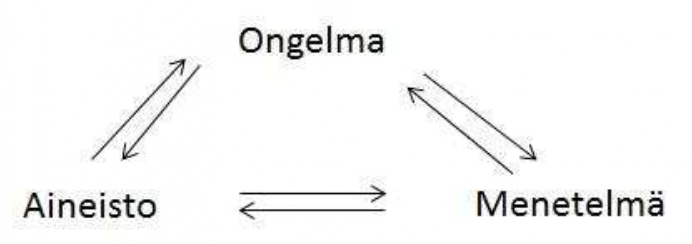
\includegraphics[width=1\linewidth]{images/tutkimusasetelma} 

}

\caption{Tutkimusasetelma}\label{fig:tutkimusasetelma}
\end{figure}

Luvussa käsiteltävät asiat kuuluvat tilastotieteelle ominaisesti kvantitatiivisen tutkimussuuntauksen alaisuuteen (ks. luku \ref{luku3}). Luvussa esiteltävät karkeat tutkimustyyppien- strategioiden ja aineistojen jaot ovat vain yksi jaottelutapa ja todennäköisesti poikkeaa eri oppikirjoissa ja lähteissä esitetyistä.

\hypertarget{alaluku101}{%
\section{Tutkimustyypit}\label{alaluku101}}

Tarkastellaan ensin erilaisia tutkimustyyppejä yleisellä tasolla. Erilaiset tutkimukset voidaan karkeasti jakaa neljään eri luokkaan: \textbf{kuvaileva}, \textbf{vertaileva}, \textbf{kokeellinen} ja \textbf{havainnoiva} tutkimus.

\begin{itemize}
\tightlist
\item
  \textbf{Kuvaileva tutkimus}

  \begin{itemize}
  \tightlist
  \item
    Tarkoituksena on kuvata jonkin ilmiön, tilanteen tai tapahtuman luonnetta, yleisyyttä, historiallista kehitystä tai muita tunnuspiirteitä mahdollisimman todenmukaisesti ja tarkasti.
  \item
    Keskeistä \textbf{tiedon lisääminen} ja pyrkimys vastata kysymyksiin \textbf{mitä}, \textbf{millainen} tai \textbf{miten}.

    \begin{itemize}
    \tightlist
    \item
      Yleisesti ottaen kuvaileva tilastollinen tutkimus perustuu aineistosta lasketuille tunnusluvuille, jotka kuvaavat aineiston ominaisuuksia. Esimerkkeinä toimivat keskiarvon lisäksi sen kaltaiset keskimääräistä havaintoa mittaavat suureet kuten mediaani ja moodi tai vaihtelua kuvaavat eri muuttujien vaihteluvälit ja keskihajonnat (ks. luku @ref\{luku6\}.
    \end{itemize}
  \item
    Saadakseen luotettavia tunnuslukuja, tulee otoksen olla edustava ja havaintojen luotettavia ja päteviä eli saatujen mittausten pitää kuvata kohteena olevaa ilmiötä ilman virheitä.
  \item
    Kuvailevassa tutkimuksessa ei tutkita muuttujien välisiä yhteyksiä tai riippuvuksia eikä täten yleensä tehdä jakoa selittäviin ja selitettäviin muuttujiin vaan muuttujat ovat asetelmallisesti samantasoisia.

    \begin{itemize}
    \tightlist
    \item
      Vastaavasti kuvailevassa tutkimuksessa ei välttämättä testata hypoteeseja, ei tehdä ennusteita, ei anneta selityksiä tai pohdita seurauksia: kyseessä on vain aineiston kuvailua ilman sen merkityksellisempää sisältöä kuten havaintojen taustalla olevien ilmiöiden tutkimista tai perusjoukon ominaisuuksien päättelyä otoksen perusteella.
    \end{itemize}
  \end{itemize}
\end{itemize}

\hfill\break

\begin{itemize}
\tightlist
\item
  \textbf{Vertaileva tutkimus}

  \begin{itemize}
  \tightlist
  \item
    Vertaileva tutkimus voidaan jakaa kahteen luokkaan

    \begin{enumerate}
    \def\labelenumi{\arabic{enumi}.}
    \tightlist
    \item
      Ryhmäeroja selittävään tutkimukseen
    \item
      Korrelaatiotutkimukseen
    \end{enumerate}
  \item
    \textbf{Ryhmäeroja selittävässä tutkimuksessa} pyritään selvittämään, mitkä tekijät liittyvät tutkittaviin ilmiöihin, jotka aiheuttavat ryhmissä ilmeneviä eroja.
  \item
    \textbf{Korrelaatiotutkimuksissa} pyritään löytämään ilmiöiden välisiä yhteyksiä tutkimalla kohdejoukkoa kokonaisuutena, jolloin mitattavien muuttujien joukkoon otetaan selittäviä muuttujia.
  \item
    Selittäviä muuttujia hyödynnetään molemmissa luokissa. Niiden avulla pyritään löytämään yhteyksiä verrattavien kohteiden välillä ja niiden voidaan ajatella olevan myös mahdollisia syitä selitettäville muuttujille, seurauksille.

    \begin{itemize}
    \tightlist
    \item
      Syy-seuraussuhteita ei kuitenkaan vertailevassa tutkimuksessa pohdita, ts. vertaileva tutkimus ei ole suoranaisesti kiinnostunut kohteena olevien ilmiöiden/ryhmien vertailussa löydettyjen erojen syistä vaan mielenkiinnon kohteena on kys. erot itsessään.
    \end{itemize}
  \item
    Vertailevaa tutkimusta tehdessä on tarpeen pohtia:

    \begin{itemize}
    \tightlist
    \item
      Miksi jotakin tutkimuskohdetta vertaillaan eli mitä tutkimuskohteesta halutaan nimenomaan saada selville.
    \item
      Mitkä ja minkälaisia tilastoyksiköitä vertailuun kannattaa ottaa mukaan, jotta tutkimuksen tavoitteet saavutetaan.
    \item
      Tyypillistä se, että kontrolli on puutteellista ja ns. väliin tulevia muuttujia ei voida aina eliminoida.
    \item
      Tutkimuksessa on hyväksyttävä myös muuttujiin liittyvä luonnollinen vaihtelu.
    \end{itemize}
  \end{itemize}
\item
  \textbf{Kokeellinen tutkimus}

  \begin{itemize}
  \tightlist
  \item
    Tarkastellaan syy-seuraussuhteita sellaisissa olosuhteissa, joissa tutkija pystyy kontrolloimaan tutkimusyksikköihin vaikuttavia tekijöitä, eli nk. ``\textbf{käsittelytekijöitä}''.
  \item
    Tavallisesti kokeellisella tutkimuksella viitataan sellaiseen tutkimukseen, jossa aineiston on kerätty valvotussa ja kontrolloidussa ympäristössä, kuten laboratoriossa tai sairaalan koehuoneissa, jotta mittaukset ja käsittelytekijät on tutkimuksen tekijän puolesta kontrolloitu ja täten halutunlaisia.

    \begin{itemize}
    \tightlist
    \item
      Tutkimusasetelman kontrollointi vähentää mittauksiin ja käsittelytekijöihin liittyvien virhelähteiden mahdollisuuksia ja täten jättää vähemmän sijaa epäilyksille.
    \item
      Lisäksi tutkimuksen toistettavuus ja objektiivisuus paranevat, kun koejärjestelyt tehdään tarkasti ja huolellisesti.
    \end{itemize}
  \item
    Kokeelliset tutkimukset tuottavat yleensä nopeammin riittävään näyttöön perustuvaa evidenssiä kuin havainnoivat tutkimukset.
  \item
    Kokeellinen tutkimusasetelma ei kuitenkaan ole mahdollinen kaikissa tilanteissa.

    \begin{itemize}
    \tightlist
    \item
      Esimerkiksi erilaisten politiikkatoimien arvioimisessa olisi hyödyllistä, mikäli se voitaisiin satunnaisesti kohdistaa esimerkiksi vain osaan kansasta tai kunnista. Tällaisten kokeilujen ehdotukset ovat kuitenkin usein kaatuneet joko perustuslaillisiin ongelmiin tasavertaisesta kohtelusta tai muihin lainsäädännöllisiin ongelmiin tai niitä ei ole toteutettu riittävän hyvin, jotta asetelma riittäisi kokeelliseen analyysiin.\footnote{Esimerkki: \href{https://labore.fi/julkaisu/kuntakokeilut-kolmas-kerta-samat-ongelmat/}{Jeremias Nieminen avaa vuonna 2020 alkaneesta työllisyyden kuntakokeilusta koeasetelman tärkeydestä politiikkatoimien arvioinnissa.}}
    \end{itemize}
  \item
    Kontrolloitujen kokeiden yleisenä kritiikkinä ja heikkoutena voidaan kuitenkin pitää niiden vähäistä yleistettävyyttä: liian pitkälle kontrolloidut ja pelkistetyt koeolosuhteet eivät toimi kaikkien tutkimuskysymysten kannalta yleistettävyyden osalta.

    \begin{itemize}
    \tightlist
    \item
      Ihmiset käyttäytyvät eri tavalla laboratorio-olosuhteissa kuin normaalissa ympäristössä!
    \end{itemize}
  \end{itemize}
\end{itemize}

\begin{eblock}{}

\textbf{Esimerkki: kasvien kasvatus eri hiilidioksidipitoisuuksissa}

\begin{itemize}
\tightlist
\item
  Hiilidioksidipitoisuuden kasvu tehostaa kasvien yhteyttämistä
\item
  Kasvit eroavat toisistaan siinä, millä tavalla ne sitovat hiilidioksidia ilmasta yhteyttämistä varten \(\rightarrow\) muutokset vaikuttavat eri tavalla eri kasveihin
\item
  Vaikuttaako ilmastonmuutos sadonmuodostukseen? Onko vaikutus suurempi joillain tietyillä kasveilla?
\end{itemize}

\end{eblock}

\FloatBarrier

\begin{figure}

{\centering 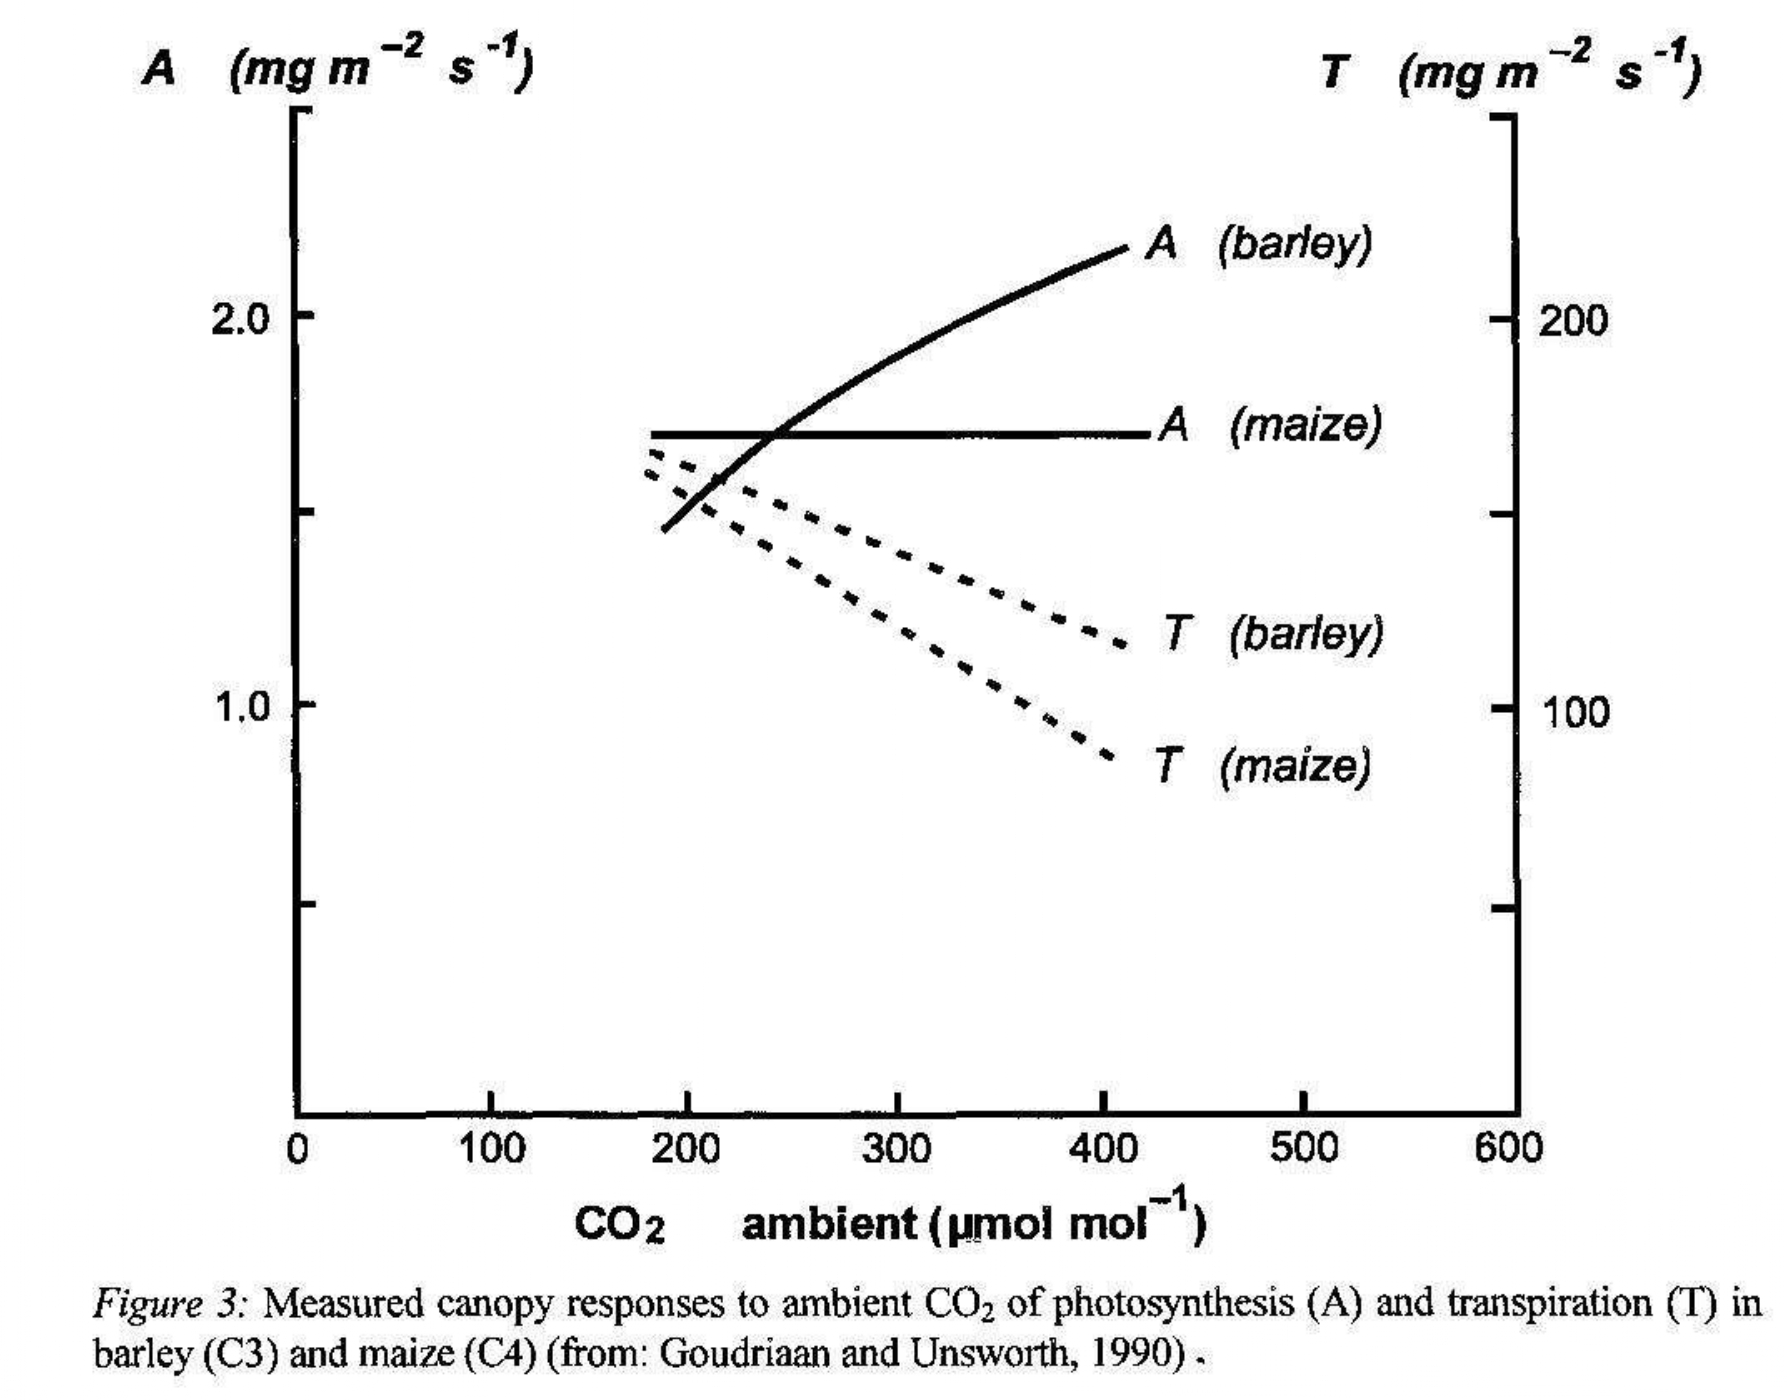
\includegraphics[width=1\linewidth]{images/co2} 

}

\caption{Hiilidioksidipitoisuuden kasvun vaikutus satomääriin.}\label{fig:co2}
\end{figure}

\FloatBarrier

\begin{eblock}{}

\textbf{Esimerkki: Lääketieteelliset kokeet}

\begin{itemize}
\tightlist
\item
  Erään tappavan taudin hoitoon on kehitetty uusi lääke, jonka toivotaan parantavan enemmän potilaita kuin kauan käytössä ollut vanha lääke. Miten saadaan varmuus siitä, että uusi lääke on parempi kuin vanha lääke?
\item
  Paranemistulosten vertailemiseksi järjestetään tilastollinen koe:

  \begin{itemize}
  \item
    \begin{enumerate}
    \def\labelenumi{(\roman{enumi})}
    \tightlist
    \item
      Jaetaan joukko potilaita arpomalla kahteen ryhmään:
    \end{enumerate}

    \begin{itemize}
    \tightlist
    \item
      Ryhmälle 1 annetaan uutta lääkettä.
    \item
      Ryhmälle 2 annetaan vanhaa lääkettä.
    \end{itemize}
  \item
    \begin{enumerate}
    \def\labelenumi{(\roman{enumi})}
    \setcounter{enumi}{1}
    \tightlist
    \item
      Verrataan parantuneiden suhteellisia osuuksia ryhmissä 1 ja 2.
    \end{enumerate}
  \end{itemize}
\item
  Kokeen tavoitteena on tehdä kokeen tulosten perusteella yleisiä johtopäätöksiä uuden lääkkeen tehokkuudesta. Miten yhdestä kokeesta saadut tulokset voidaan yleistää koskemaan kaikkia tautia sairastavia potilaita?

  \begin{itemize}
  \tightlist
  \item
    Kokeen tulokset voidaan yleistää, jos kokeessa uutta ja vanhaa lääkettä saavien potilaiden ryhmät ovat samankaltaisia kaikissa muissa suhteissa paitsi siinä, että niihin kohdistetaan kokeessa erilainen käsittely.

    \begin{itemize}
    \tightlist
    \item
      Tällöin mahdolliset erot parantuneiden suhteellisissa osuuksissa on oltava seurausta erilaisista käsittelyistä.
    \item
      Kokeen kohteiden jakaminen ryhmiin arpomalla on ainoa menetelmä, joka mahdollistaa samankaltaisten ryhmien saamisen.
    \item
      Kokeen kohteiden jakamista erilaisen käsittelyn kohteiksi joutuviin ryhmiin arpomalla kutsutaan siis \textbf{satunnaistamiseksi}.
    \end{itemize}
  \item
    Arvonnan käyttö ryhmiin jaossa merkitsee sitä, että koetulokset ovat satunnaisia seuraavassa mielessä: Jos arvontaa toistettaisiin, kokeesta saataisiin (suurella todennäköisyydellä) erilaiset ryhmäjaot.
  \end{itemize}
\item
  Kysymyksiä:

  \begin{itemize}
  \tightlist
  \item
    Miten yhdestä kokeesta saadut ja satunnaiset koetulokset voidaan yleistää koskemaan kaikkia ko. tautia sairastavia potilaita?
  \item
    Miten luotettava tällainen yleistys on?
  \end{itemize}
\item
  Vastauksia:

  \begin{itemize}
  \tightlist
  \item
    Jos potilaiden jaossa ryhmiin on käytetty satunnaistamista, kokeen tuloksiin sisältyvälle epävarmuudelle ja satunnaisuudelle voidaan muodostaa tilastollinen malli, joka mahdollistaa sekä koetulosten yleistämisen että yleistyksen luotettavuuden arvioimisen.
  \end{itemize}
\item
  Yleistyksen luotettavuutta ei pystytä arvioimaan, ellei ryhmiin jaossa ole käytetty satunnaistamista.
\item
  Tilastollisen kokeen suunnittelussa, toteutuksessa ja tulosten analysoinnissa sovelletaan mm. seuraavia tilastollisia menetelmiä: koesuunnittelu, estimointi ja testaus.
\end{itemize}

\end{eblock}

\hfill\break

\begin{itemize}
\tightlist
\item
  \textbf{Havainnoiva tutkimus}

  \begin{itemize}
  \tightlist
  \item
    Kuten edellä mainittiin, kokeellisia tutkimusasetelmia ei useinkaan ole mahdollista järjestää. Tällaisia kysymyksiä voidaan kuitenkin tutkia havainnoivassa tutkimuksessa, jossa syy-seuraussuhteita tarkastellaan tilanteissa, joissa tutkijalla ei ole välttämättä mitään kontrollia (tai syytä sille) tutkimusyksikköihin tai heihin vaikuttaviin muuttujiin (käsittelytekijöihin).

    \begin{itemize}
    \tightlist
    \item
      Esimerkiksi tutkimusasetelmat, joissa tutkimuksen kohteena olevia yksiköitä (esim. ihmiset, kunnat, valtiot) ei voida satunnaistaa kuuluvaksi osaksi joukkoa, joka altistetaan jollekin käsittelylle.
    \end{itemize}
  \item
    Tällöin tutkijan on tyydyttävä havainnoimaan sitä mitä tapahtuu luonnostaan tietyssä (mahdollisesti satunnaisesti poimitussa) tutkimusjoukossa tietyssä tilanteessa.
  \item
    Havainnoivan tutkimuksen aineistoa voidaan analysoida samoin menetelmin kuin kokeellisen tutkimuksenkin, mutta mitattujen tekijöiden vaikutusta ei voida erottaa kokonaisuudesta samalla tarkkuudella kuin kokeellisessa tutkimuksessa.
  \item
    Havainnoivan tutkimuksen tilastollinen teoria muodostuu periaatteista ja menetelmistä, joiden avulla aineiston tuottaman evidenssin painoarvoa voidaan arvioida mahdollisimman ``puhtaasti''.
  \item
    \textbf{Havainnoivan tutkimuksen edut}

    \begin{itemize}
    \tightlist
    \item
      Saadaan välitöntä ja suoraa tietoa yksilöiden, ryhmien ja organisaatioiden toiminnasta ja käyttäytymisestä.
    \item
      Tutkija voi havainnoida tutkittavia luonnollisessa ympäristössä.
    \item
      Sopii sekä määrällisen että laadullisen aineiston hankkimiseen.
    \item
      Erinomainen menetelmä muun muassa vuorovaikutuksen tutkimisessa, ja silloin kun tilanteet ovat vaikeasti ennakoitavia ja nopeasti muuttuvia.
    \item
      Sopii myös silloin, kun tutkittavilla on kielellisiä vaikeuksia (kuten lapset) tai kun halutaan saada selville sellaista tietoa, jota tutkittavat eivät halua suoraan kertoa tutkijalle.
    \end{itemize}
  \item
    \textbf{Havainnoivan tutkimuksen haitat}

    \begin{itemize}
    \tightlist
    \item
      Tutkija saattaa häiritä tilannetta tai muuttaa sen kulkua.
    \item
      Tutkija saattaa sitoutua emotionaalisesti tutkittavaan ryhmään tai tilanteeseen.
    \end{itemize}
  \end{itemize}
\end{itemize}

\begin{eblock}{}

\textbf{Esimerkki: raskauden keskeytyksen ja rintasyövän välinen kausaaliyhteys}

\begin{itemize}
\tightlist
\item
  Kokeellinen asetelma: Poimitaan satunnaisesti \(n\) kappaletta raskaana olevia naisia ja heistä \(n_1\) kappaletta satunnaistetaan käsittelyryhmään (raskauden keskeytys) ja \(n_2\) kontrolliryhmään. Kaikki naiset käyvät muutaman seuraavan vuoden ajan syöpäseulonnoissa.
\item
  Kokeelliseen asetelma ei selvästikään ole eettisistä syistä mahdollinen, eikä sitä olisi mahdollista suorittaa sokkoutettuna kokeena
\item
  Aiheesta julkaistut tutkimukset aloittavat yleensä naisista, joille on jo tehty raskauden keskeytys
\item
  Käsittelyryhmään kuuluminen ei siis ole tutkijan kontrollissa
\end{itemize}

\end{eblock}

\hfill\break

\begin{eblock}{}

\textbf{Esimerkki: lääkityksen aiheuttama harvinainen sivuvaikutus}

\begin{itemize}
\tightlist
\item
  Harvinaisen ilmiön tarkastelu satunnaistetulla kokeella on epäkäytännöllistä, sillä saattaa olla, että isossakaan tutkimusjoukossa sivuvaikutusta ei esiinny yhdelläkään tutkittavalla
\item
  Havainnoiva tutkimus aloittaisi tässä tapauksessa etsimällä ensin sivuvaikutuksesta kärsivät potilaat ja sen jälkeen selvittäisi ketkä heistä ovat saaneet kyseistä lääkettä (ja saaneet sivuoireet lääkityksen aloittamisen jälkeen)
\end{itemize}

\end{eblock}

\hypertarget{alaluku102}{%
\section{Tutkimusstrategiat}\label{alaluku102}}

\begin{itemize}
\tightlist
\item
  Erilaiset tutkimusasetelmat voidaan jakaa edelleen kahteen \textbf{tutkimusstrategiaan} sen mukaan, miten niissä ryhmitellään tilastoyksiköitä: \textbf{poikkileikkaus}- ja \textbf{pitkittäistutkimuksiin}. Tilastoyksikköjen erilainen ryhmittely tuottaa erilaisia aineistotyyppejä, jotka voidaan jaotella karkeasti kolmeen eri tyyppiin

  \begin{itemize}
  \tightlist
  \item
    Poikkileikkausaineistot: havaintoaineisto kattaa yhden ajankohdan ja mahdollisesti useita tilastollisia muuttujia
  \item
    Aikasarja-aineistot: havaintoaineisto kattaa vain yhden tilastollisen muuttujan mitattuna useana ajanhetkenä
  \item
    Paneeliaineistot: havaintoaineisto kattaa mahdollisesti useita tilastollisia muuttujia mitattuna useana ajanhetkenä
  \end{itemize}
\item
  Eri tutkimusstrategiat hyödyntävät eri aineistotyyppejä sen mukaan, miten ne sopivat tutkimuskysymykseen ja valittuun menetelmään. Tarkastellaan seuraavaksi mitä em. kaksi tutkimustrategiaa tarkoittavat, miten ne eroavat ja minkälaisia tutkimustyyppejä-, asetelmia- ja aineistoja kumpaankin kuuluu.
\end{itemize}

\hypertarget{poikittaistutkimus-eli-poikkileikkaustutkimus}{%
\subsection{\texorpdfstring{\textbf{Poikittaistutkimus} eli \textbf{poikkileikkaustutkimus}}{Poikittaistutkimus eli poikkileikkaustutkimus}}\label{poikittaistutkimus-eli-poikkileikkaustutkimus}}

\begin{itemize}
\tightlist
\item
  Poikittaistutkimukseksi kutsutaan tutkimusstrategiaa, jossa tarkoituksena on tutkia kohdetta tai ilmiötä laaja-alaisesti tiettynä ajankohtana käyttäen poikkileikkausaineistoja.

  \begin{itemize}
  \tightlist
  \item
    Voidaan tarkastella useita ryhmiä, joissa on esimerkiksi eri-ikäisiä henkilöitä ja ryhmistä saatua tietoa vertaillaan toisiinsa.
  \item
    Voidaan käyttää kuvailemaan riskisuhteita (odds ratio) tai kuvailemaan tiettyyn populaation osaan kohdistuvaa ilmiötä tai riskiä (esimerkiksi sydän- ja verisuonitaudit).

    \begin{itemize}
    \tightlist
    \item
      Esimerkiksi tutkittaessa sydän- ja verisuonitauteja binäärisellä vastemuuttujalla käyttäen aineistoa, joka koostuu eri ikäisistä ja kuntoisista ihmisistä voidaan arvioida iän ja muiden muuttujien vaikutuksia sydän- ja verisuonitauteihin sairastumisen riskitekijöinä.
    \end{itemize}
  \item
    Poikittaistutkimuksessa ei saada tietoa tilastoyksikön mielenkiinnon kohteena olevien muuttujien arvojen muutoksesta yli ajan mutta tutkimuksessa voidaan kuitenkin kerätä tietoa menneisyyteen liittyen.
  \item
    Eri ikäryhmiä vertailtaessa ongelmana on myös niin sanottu kohorttivaikutus: tiettynä aikana syntyneiden, eli tietyn kohortin, elinolosuhteet saattavat olla täysin erilaiset kuin jonakin toisena aikana syntyneiden, minkä vuoksi ikäryhmien väliset erot saattavat johtua esimerkiksi yhteiskunnallisista olosuhteista.
  \item
    Poikittaistutkimukseen osallistutaan vain yhden kerran, jolloin tietoa saadaan kerralla paljon.

    \begin{itemize}
    \tightlist
    \item
      Tämä on kuitenkin usein työlästä ja suuren poikkileikkausaineston kerääminen voi olla kallista.
    \item
      Poikittaistutkimuksessa hyödynnetäänkin usein rutiinitoimenpiteinä kerättyjä aineistoja (esimerkiksi tietyn ikävuoden terveystarkastuksista)
    \item
      Näin voidaan selvittää korrelaatioita ilmiöiden välillä (esimerkiksi alkoholin käyttö ja maksakirroosi) ja siten luoda hypoteeseja tarkemmille jatkotutkimuksille
    \item
      Tällöin on kuitenkin taas vaara sekoittavista tekijöistä, jos aineistoa ei ole kerätty varta vasten tätä tarkoitusta varten
    \end{itemize}
  \end{itemize}
\end{itemize}

\begin{figure}

{\centering 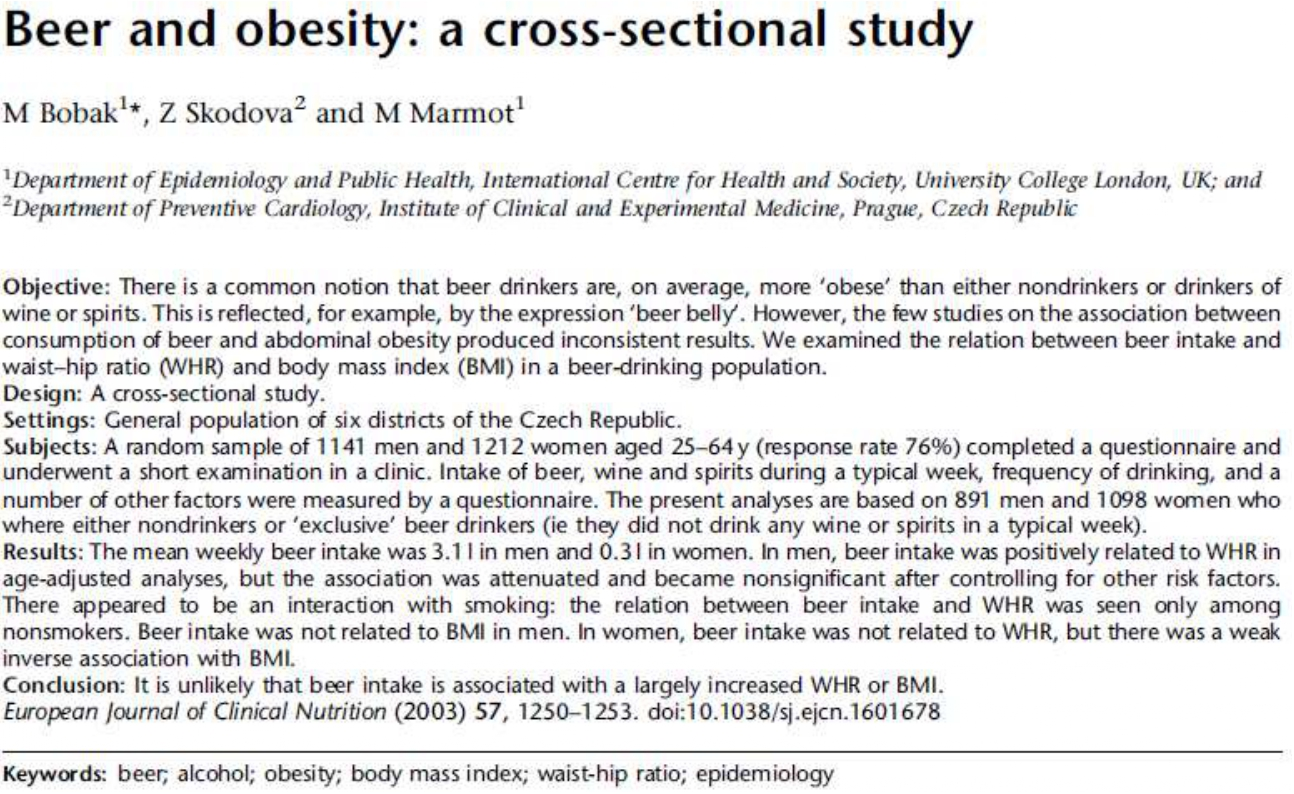
\includegraphics[width=1\linewidth]{images/cross} 

}

\caption{Esimerkki poikkileikkaustutkimuksesta}\label{fig:cross}
\end{figure}

\hfill\break

\hypertarget{pitkittuxe4istutkimus}{%
\subsection{\texorpdfstring{\textbf{Pitkittäistutkimus}}{Pitkittäistutkimus}}\label{pitkittuxe4istutkimus}}

\begin{itemize}
\tightlist
\item
  Pitkttäistutkimuksessa seurataan usein samoja tilastoyksiköitä ``yli ajan'', eli mittauspisteitä on useita ja pitkältä aikaväliltä.

  \begin{itemize}
  \tightlist
  \item
    Hyödyntää poikkileikkausdimension lisäksi myös aikasarjadimensiota.
  \item
    Yleinen tutkimuskysymys pitkittäistutkimuksessa on jonkin \textbf{käsittelyn vaikutuksen arviointi}. Tällaisia ovat esimerkiksi lääkeainetutkimus, poliittisten päätösten arviointi tai markkinointitutkimus.

    \begin{itemize}
    \tightlist
    \item
      Pitkittäistutkimuksessa voidaan siis tarkastella \textbf{muutosta} mutta on tärkeä muistaa, että pitkittäistutkimuksen eri mittauskerrat eivät ole toisistaan \textbf{riippumattomia} ja tämä tulee ottaa tilastollisessa mallissa huomioon!
    \end{itemize}
  \item
    Pitkittäistutkimuksen hyvänä puolena on \textbf{ryhmien homogeenisyys}

    \begin{itemize}
    \tightlist
    \item
      Tutkittavan ryhmän henkilöt ovat eläneet saman historiallisen ajan sekä käyneet läpi samat yhteiskunnalliset muutokset, jolloin muutoksen tutkiminen on luotettavaa, sillä tutkimusta vääristävät tilastoyksiköiden ominaisuuksista erilliset ympäristön haittamuuttujat ovat kaikille samat.
    \item
      Pitkittäistutkimuksen pitkän keston vuoksi tutkittavien määrää kuitenkin yleensä vähenee ja tutkimuksen valmistumisessa kestää kauan, jopa vuosikymmeniä.
    \end{itemize}
  \end{itemize}
\end{itemize}

\begin{figure}

{\centering 
\includegraphics[width=1\linewidth]{images/long} 

}

\caption{Esimerkki pitkittäistutkimuksesta}\label{fig:long}
\end{figure}

\newpage

\begin{eblock}{}

\textbf{Esimerkki: poikittais- ja pitkittäistutkimus epidemiologiassa}

\begin{itemize}
\tightlist
\item
  Epäkokeelliset epidemiologiset tutkimukset voivat olla joko poikittaistutkimuksia tai pitkittäistutkimuksia.
\item
  Poikittaistutkimus on tiettyyn ajankohtaan rajoittuva tutkimus, jossa mitataan sairauksien vallitsevuutta eli prevalenssia.

  \begin{itemize}
  \tightlist
  \item
    Prevalenssi kuvaa sairauden tai haitan omaavien henkilöiden määrää tarkasteltavasta väestöstä tiettynä ajankohtana.
  \item
    Usein mitataan vallitsevuustiheyttä eli sairaiden lukumäärää tiettynä ajanhetkenä / väkiluku samana ajankohtana.
  \end{itemize}
\item
  Pitkittäistutkimuksessa mitataan sairauksien ilmaantuvuutta eli insidenssiä.

  \begin{itemize}
  \tightlist
  \item
    Tutkimuksessa seurataan väestössä ilmaantuvien uusien sairaustapausten lukumäärää tietyn ajanjakson aikana.
  \item
    Useimmiten mitataan ilmaantuvuustiheyttä, joka ilmoittaa uusien sairastapausten määrän henkilöaikaa kohden.
  \item
    Henkilöaika muodostuu tarkasteltavan henkilöryhmän yhteenlasketusta seuranta-ajasta ennen sairastumista, esimerkiksi 100 henkilövuotta muodostuu seurattaessa 100 henkilöä vuoden ajan tai 10 henkilöä 10 vuoden ajan.
  \end{itemize}
\end{itemize}

\end{eblock}

\hfill\break

\hypertarget{kohorttitutkimus}{%
\subsection{\texorpdfstring{\textbf{Kohorttitutkimus}}{Kohorttitutkimus}}\label{kohorttitutkimus}}

\begin{itemize}
\tightlist
\item
  Kohorttitutkimus on altistelähtöinen tapa toteuttaa pitkittäistutkimus.

  \begin{itemize}
  \tightlist
  \item
    \textbf{Kohortti} on suljettu väestö (syntymäkohortti, tietyn työpaikan työntekijät, yms.), jota tutkimuksessa seurataan ja joka on valittu jonkin yhteisen ominaisuuden perusteella (syntymävuosi, työpaikka, yms.).

    \begin{itemize}
    \tightlist
    \item
      Kohortti voidaan jakaa myös alakohortteihin, mikäli se on alkujaankin riittävän suuri.
    \item
      Valitun kohortin tilastoyksiköt pyritään pitämään täysin samana koko tutkimuksen ajan, ts. kohortit ovat kiinteitä.
    \end{itemize}
  \item
    Tutkimuksessa voidaan valita esimerkiksi jollekkin käsittelymuuttujalle altistunut ja altistumattomien ryhmä.

    \begin{itemize}
    \tightlist
    \item
      Kohortin seuranta-aikana tutkitaan ryhmien välillä ilmeneviä eroja mielenkiinnon kohteena olevassa muuttujassa.
    \item
      Näitä voi olla esimerkiksi ryhmien väliset erot sairastuvuudessa, kun käsittely on ollut jokin lääke kuten rokote tms. Vastaava esimerkki olisi em. työllisyyden kuntakokeilun osalta työllisyysaste eri kunnissa ja erojen tutkiminen kuntakokeiluun osallistuvien ja osallistumattomien välillä.
    \end{itemize}
  \item
    Kohorttitukimus voi olla \textbf{taannehtiva}: tutkija määrittelee kohortin menneisyydessä, ja seuraa olemassaolevien rekisterien avulla, mitä kohortin jäsenille on tapahtunut myöhemmin.
  \item
    Kohorttitutkimuksessa voidaan yleensä tutkia kerrallaan vain \textbf{yhtä altistetta/käsittelyä}, mutta \textbf{useita tilastollisia muuttujia}.
  \item
    Tutkimukset saattavat olla hyvin pitkäkestoisia, jos tutkitaan ilmiötä, joka ilmenee vasta pitkä ajan kuluttua altistuksesta (kuten sairaus tai työllisyyden paraneminen)
  \item
    Kohorttitutkimus voi vastata kysymykseen: ``Mitkä ilmiöt johtuvat tästä altisteesta?''
  \end{itemize}
\end{itemize}

\begin{eblock}{}
\textbf{Esimerkki kohorttitutkimuksesta}

Toisen maailmansodan aikana räjäytettiin Japanissa kaksi atomipommia. Tämän traagisen tapahtuman jälkeen tutkijat alkoivat selvittää, mitä terveysvaikutuksia ionisoiva säteily aiheuttaisi altistuneille. Tutkimuksessa seurattiin altistuneiden ja altistumattomien sairastumista vuodesta 1945 vuoteen 1970. Tutkimuksen mukaan ionisoiva säteily aiheutti etupäässä monenlaisia kasvaimia; mm. keuhkosyöpää, rintasyöpää ja kilpirauhasen syöpää.

\end{eblock}

\begin{figure}

{\centering 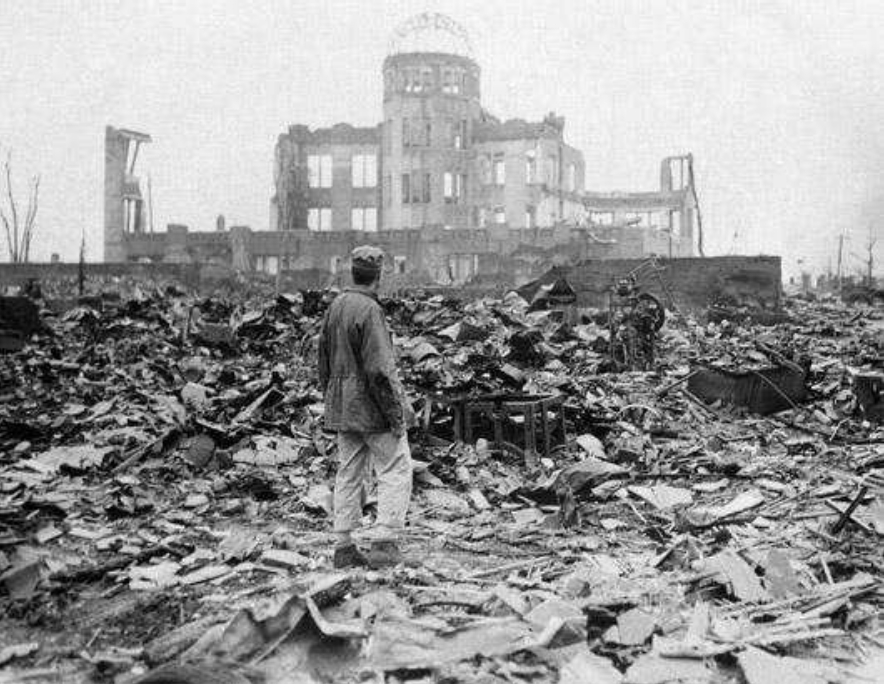
\includegraphics[width=1\linewidth]{images/hiroshima} 

}

\caption{Yhdysvaltain räjäyttämä atomipommi Japanin Hiroshimassa aiheutti mittaamattomia tuhoja.}\label{fig:hiroshima}
\end{figure}

\hfill\break

\hypertarget{tapaus-verrokkitutkimus}{%
\subsection{\texorpdfstring{\textbf{Tapaus-verrokkitutkimus}}{Tapaus-verrokkitutkimus}}\label{tapaus-verrokkitutkimus}}

\begin{itemize}
\tightlist
\item
  On \textbf{retrospektiivinen havainnoiva} pitkittäistutkimusmenetelmä, jossa tutkimukseen valitaan esimerkiksi tutkittavaan sairauteen (tai muulle altisteelle/käsittelylle altistuneita) potilaita (\textbf{tapaukset}) ja lisäksi henkilöitä, jotka eivät ole sairastuneita tähän sairauteen (\textbf{verrokit}) (tai altistuneet altisteelle/käsittelylle).

  \begin{itemize}
  \tightlist
  \item
    Tavoitteena on tutkia miten tutkimusyksiköt reagoivat altistuttuaan jollekin altisteelle tai käsittelylle. Soveltuu erityisesti harvinaisten ilmiöiden aiheuttajien selvittämiseen.

    \begin{itemize}
    \tightlist
    \item
      Esimerkkinä altistuminen Covid-19 virukselle: retrospektiivisesti (jälkikäteen) voidaan tarkastella viruksen kantajan kanssa samassa tilassa olleita (virukselle altistuneita (virus on altiste)) kyseisessä tilassa olleet olisivat tapauksia ja hypoteettinen toinen tila ilman virusta toimisi verrokkina (ts. ei yhtäkään tartuntatapausta). Mielenkiinnon kohteena olisi tarkastella kuinka monta henkilöä sai tartunnan (ja minkälaiset olosuhteet olivat).
    \item
      Toisena esimerkkinä voitaisiin jälleen pitää em. työllisyyden kuntakokeilua: ne kunnat jotka (satunnaisesti) valikoituisivat työllisyyskokeiluun tulisivat altistetuksi politiikkamuutokselle eli olisivat tapauskuntia. Näitä kuntia voidaan sitten verrata verrokkikuntiin, joissa kys. politiikkamuutosta ei toteutettaisi. Mielenkiinnon kohteena olisi työllisyyden kehitys altistumisen jälkeen.
    \end{itemize}
  \item
    Käsittelyn tai altistuksen seurauksia, esimerkiksi sairauden, syitä etsitään vertaamalla tapausten ja verrokkien aikaisempaa altistumista erityisesti mielenkiinnon kohteena oleville altisteille.
  \item
    Tapaus-verrokkitutkimus eroaa kohorttitutkimuksesta siten että siinä voidaan tutkia \textbf{yhtä tilastollista muuttujaa} (kuten sairastumista), mutta \textbf{useita altisteita}: mistä altisteesta sairaus on seuraus, ts. mikä on taudinaiheuttaja?

    \begin{itemize}
    \tightlist
    \item
      Altistumishistoriaa voidaan selvitettää mm. mittauksilla, malleilla tai kyselylomakkeilla.
    \item
      Esimerkki: tapauksien ja verrokkien altistumiseroista saadaan epäsuora arvio altistuneiden riskistä sairastua kyseiseen sairauteen suhteessa altistumattomien riskiin.
    \end{itemize}
  \item
    Tapaus-verrokkitutkimukset ovat yleensä suhteellisen yksinkertaisia ja halpoja toteuttaa niiden retrospektiivisestä luonteesta johtuen: tutkimuskysymys määrittelee aineistotarpeen, jonka jälkeen se tarvitsee vain kerätä.

    \begin{itemize}
    \tightlist
    \item
      Verrokkien valinta kuitenkin kriittinen, sillä valitsemalla verrokit/kontrollitapaukset väärin mikään tilastollinen testi tai menetelmä ei korjaa tai kvantifioi tätä virhettä!
    \item
      Esimerkki verrokkiryhmän epäkelvosta valinnasta on huonosti mitattu aiempi altistuminen ja/tai jos jokin tutkimuksen kannalta keskeinen taustamuuttuja sivuutetaan: mitä jos tauti tai sen vakavuus riippuukin sairastuneen muusta terveydentilasta?
    \end{itemize}
  \item
    Eroaa poikittaistutkimuksesta siinä, että poikittaistutkimus pyrkii yleistämään tulokset koko kohdepopulaatioon, kun taas tapaus-verrokkitutkimus keskittyy hyvin spesifiin populaation osaan
  \end{itemize}
\end{itemize}

\begin{eblock}{}
\textbf{Esimerkki: tapaus-verrokkitutkimuksesta}

Länsi-Saksassa tuotiin 50-luvun lopulla markkinoille talidomidi-niminen uni- ja rauhoittava lääke. Varsin pian markkinoille tulon jälkeen tietyntyyppisten synnynnäisten epämuodostumien määrä alkoi lisääntyä rajusti. Talidomidin ja lasten raajojen muodostumishäiriöiden yhteys paljastettiin tapaus-verrokkitutkimuksilla. Tutkimuksissa selvitettiin sekä sairaiden lasten (tapaukset) että terveiden lasten (verrokkien) äitien altistuminen talidomidille raskauden kriittisten viikkojen aikana. Melkein kaikki sairaiden lasten äidit olivat saaneet talidomidia ensimmäisten raskausviikkojen aikana (talidomidin oli myös havaittu helpottavan odottavien äitien raskauspahoinvointia). Talidomidi poistettiin markkinoilta ja epämuodostumatapausten määrä putosi jyrkästi.

\end{eblock}

\begin{figure}

{\centering 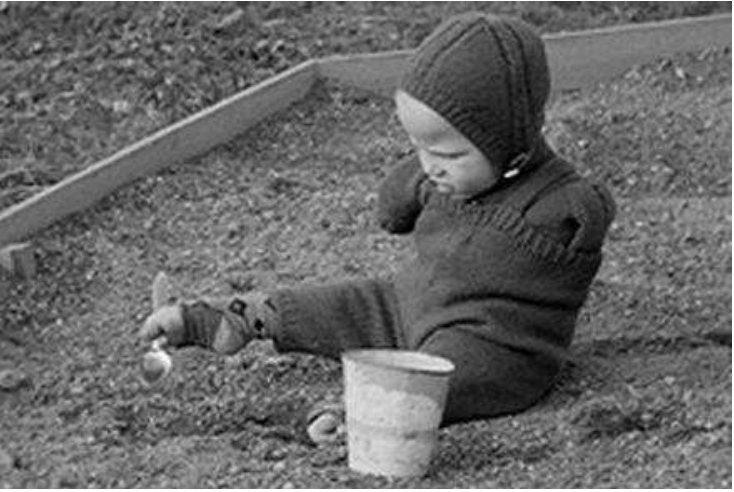
\includegraphics[width=1\linewidth]{images/tali} 

}

\caption{Esimerkki tapaus-verrokkitutkimuksesta}\label{fig:tali}
\end{figure}

\hfill\break

\begin{itemize}
\tightlist
\item
  \textbf{Lohkot/osittaminen}

  \begin{itemize}
  \tightlist
  \item
    Lohkomisella / osittamisella tarkoitetaan tutkimusyksiköiden järjestämistä ryhmiin niin, että ryhmät ovat mahdollisten sekoittavien tekijöiden suhteen mahdollisimman samankaltaiset
  \item
    Lohkotekijä on yleensä muuttuja, jonka aiheuttama vaihtelu vasteeseen ei ole tutkijan päämielenkiinnon kohteena
  \item
    Lohkotekijän kontrollointi johtaa usein tarkkuudeltaan parempiin tuloksiin
  \item
    ``Block what you can, randomize what you cannot.''
  \end{itemize}
\end{itemize}

\begin{figure}

{\centering 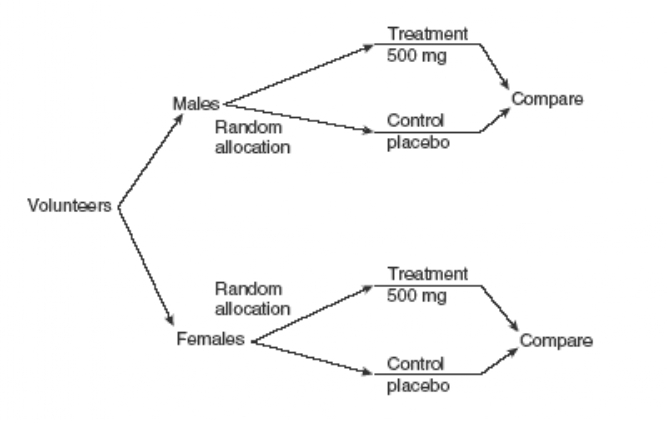
\includegraphics[width=1\linewidth]{images/block} 

}

\caption{Esimerkki ositetusta koeasetelmasta}\label{fig:block}
\end{figure}

\begin{itemize}
\tightlist
\item
  \textbf{Sokkouttaminen}

  \begin{itemize}
  \tightlist
  \item
    Tutkimushoitojen sokkoutuksen tavoitteena on vähentää sekä potilaan että tutkimushenkilökunnan mahdollisten ennakkokäsitysten vaikutusta tutkimuksen tuloksiin.
  \item
    \textbf{Yksöissokkotutkimuksessa} (single-blind) tutkittava ei tiedä, mihin hoitoryhmään hän kuuluu.
  \item
    \textbf{Kaksoissokkotutkimuksessa} (double-blind) ei tutkittava eikä tutkija ja muukaan tutkimushenkilökunta saa tutkimuksen aikana tietää mihin hoitoryhmään tutkittava kuuluu.
  \item
    \textbf{Kolmoissokkoutetussa} tutkimuksessa edes havaintojen analysoija (esim. tilastotutkija) ei tiedä, miten kokeellisen tutkimuksen käsittely on koodattu.
  \item
    \textbf{Avoimessa tutkimuksessa} (open) sekä tutkittava että tutkimushenkilökunta tietävät, mihin hoitoryhmään tutkittava kuuluu. Myös avoimessa tutkimuksessa tulisi yleensä käyttää satunnaistamista.
  \end{itemize}
\end{itemize}

\hypertarget{alaluku103}{%
\section{Erilaisia aineistoja ja aineistolähteitä}\label{alaluku103}}

Käydään seuraavaksi läpi erilaisia aineistotyyppejä, joita käytännön tutkimuksissa Suomessa (ja maailmalla) usein käytetään. Emme käsittele tässä erikseen itse otannalla koottavia aineistoja tai otannan järjestämistä, ks. luku \ref{luku5}.

\hypertarget{rekisteriaineistot}{%
\subsection{Rekisteriaineistot}\label{rekisteriaineistot}}

\begin{itemize}
\item
  Rekisteriperusteinen tutkimus hyödyntää aineistoinaan valmiiksi kerättyjä \textbf{tietokantoihin} tallennettuja aineistoja, joita kutsutaan rekisteriaineistoiksi.

  \begin{itemize}
  \tightlist
  \item
    Yleensä \textbf{hallinnollisia tarpeita} varten kerättyjä tietoja.
  \end{itemize}
\item
  Rekisteriaineistojen eduiksi voidaan lukea mm. seuraavat seikat

  \begin{itemize}
  \tightlist
  \item
    Aineiston muodostaminen/kerääminen on verrattain helppoa ja Suomessa on paljon korkealaatuisia rekisteriaineistoja. Tätä edesauttaa tietotekniikan nopea kehittyminen, joka on mahdollistanut erittäin suurten aineistojen rutiininomaisen keräämisen.
  \item
    Ei tarvetta erikseen tuottaa tutkimusaineistoa: vältetään mahdollisesti kallis aineiston keräysvaihe.
  \item
    Suomalainen henkilötunnusjärjestelmä mahdollistaa tietojen tehokkaan käytön ja laadukkaan tutkimuksen.
  \end{itemize}
\item
  Rekisteriaineistojen ongelmina ja haittoina voidaan pitää mm. seuraavia

  \begin{itemize}
  \tightlist
  \item
    Mikäli tutkimuksessa lähtökohtaisesti käytetään rekisteriaineistoja, määräävät ne välillisesti myös mahdolliset tutkimuskohteet: rekisteriaineistot kerätään eri tarkoitusta varten eivätkä ne täten välttämättä sisällä kaikkea haluttua informaatiota.

    \begin{itemize}
    \tightlist
    \item
      Tutkimuksen ongelmalähtöisyys saattaa unohtua helpommin, kun tutkimusongelman aihiota asetellaan sopimaan rekisteriaineistojen tarjoamiin mahdollisuuksiin.
    \item
      Rekisteriaineistoilla on myös omat rajansa: tutkimuskysymysten kannalta väärin mitattua muuttujaa ei useinkaan voida millään tavalla muuntaa täydellisesti haluttuun muotoon.
    \end{itemize}
  \item
    Rekisteriaineisto pitää usein esikäsitellä sopivaan muotoon laadullista tutkimusta muistuttavalla tavalla.
  \item
    Rekisteriaineistojen analyysista ja niihin soveltuvista tilastollisista menetelmistä on vähänlaisesti metodologisia oppikirjoja ja/tai esimerkkitutkimuksia.
  \item
    ``Ulkopuolisille'' tutkijoille aineistojen käyttö saattaa olla hankalaa mm. korkeiden pääsykustannusten (rekisterien ylläpitäjien, viranomaisten ja tutkimuslaitosten ulkopuolella), tietosuojakysymysten tai teknisten hankaluuksien takia.

    \begin{itemize}
    \tightlist
    \item
      Rekisteriaineiston käyttö vaatii tutkimussuunnitelman ja tutkimussuunnitelman perusteella myönnetyn käyttöluvan rekisterin ylläpitäjältä.
    \end{itemize}
  \item
    Tietotekniikan kehittymisen vuoksi kasvaneet rekisteriaineistot tekevät käyttökelpoisen tiedon esiin seulomisesta haastavaa. Tämä näyttäytyy esimerkiksi eri rekistereiden tietojen linkkaamista yhteen, jolla saattaa olla tutkimuksen kannalta ratkaiseva merkitys ja joka edelleen korostaa substanssitietoutta.

    \begin{itemize}
    \tightlist
    \item
      Eri rekisterejä ei aina saadakaan linkattua tehokkaasti yhteen esimerkiksi jos ne ovat mitanneet mielenkiinnon kohteina olevia muuttujia eri tilastoyksikön tasolla (vrt. kunnan vs kaupunginosan työllisyys)
    \end{itemize}
  \end{itemize}
\item
  Erilaisia rekisterejä Suomessa:

  \begin{itemize}
  \tightlist
  \item
    Verorekisterit (Verohallinnon rekisterit)
  \item
    Kuolemansyyrekisterit
  \item
    Eläkerekisterit
  \item
    Väestölaskennat (väestörekisteri)
  \item
    Syöpärekisteri
  \item
    Lääkeostorekisteri
  \item
    Sosiaali- ja terveydenhuollon rekisterit
  \item
    Kelan etuusrekisterit
  \item
    Osoiterekisterit
  \item
    Etukorttirekisterit
  \item
    Opintosuoritusrekisteri
  \end{itemize}
\item
  Näiden lisäksi tulevat myös aikaisempien tutkimusten aineistot.
\item
  Rekisteriaineiston käyttämisen \textbf{tilastollisia haasteita} tutkimuksessa

  \begin{itemize}
  \tightlist
  \item
    Rekisteriaineistot ovat usein kokonaisaineistoja, joten otantavirheeseen perustuvan tilastollisen päättelyn oletukset eivät välttämättä päde.

    \begin{itemize}
    \tightlist
    \item
      Isoissa aineistoissa käytännössä merkityksettömistäkin eroista tulee helposti tilastollisesti merkitseviä!
    \end{itemize}
  \end{itemize}
\item
  Rekisteriaineistoja saadaan ``valmiina'' ja niiden kokonaistutkimukseen soveltuvasta luonteesta huolimatta niitä on arvioitava samojen periaatteiden mukaisesti kuin itse kerättäviäkin aineistoja.

  \begin{itemize}
  \tightlist
  \item
    Tutkimusongelman pitäisi aina olla keskeinen lähtökohta myös rekisteriaineiston käytössä.
  \item
    Itse kerätessä aineisto on mahdollista räätälöiden tuottaa vastaamaan juuri tutkimuskysymykseen kun taas rekisteriaineisto on ``toisen käden'' aineistoa ja ohjaa täten tutkimusta niin käsitteiden määrittelystä kuin tutkimuskysymysten asettelusta lähtien.
  \end{itemize}
\item
  \textbf{Tietosuojalaki}: Lain mukaan henkilötietoja voidaan kerätä ja tallettaa vain, jos rekisterinpitäjän ja rekisteröitävän henkilön välillä on asiallinen yhteys. Olennaista lain soveltamisessa on, voidaanko käytössä olevan aineiston tiedot tosiasiassa tavalla tai toisella liitää tiettyyn tunnistettavissa olevaan henkilöön.

  \begin{itemize}
  \tightlist
  \item
    Lain merkitys on paljolti siinä, että se ohjaa suunnitelmallisuuteen ja huolellisuuteen henkilötietojen käsittelyssä.
  \item
    Sääntelyjen yleisenä tavoitteena on ettei tarpeettomasti kerätä ja talleteta henkilötietoja ettei rekisteröityjen yksityisyyttä ja oikeuksia perusteettomasti loukata ja että rekisteri, siihen liittyvät tiedot ja niiden käsittely suojataan kaikissa vaiheissa.
  \end{itemize}
\item
  Rekisteriaineistot tietosuojalain takaaman yksityisyydensuojan näkökulmasta

  \begin{itemize}
  \tightlist
  \item
    Suomessa rekisteriaineistot pyritään luovuttamaan käyttöön vain tunnisteettomina yksityisyydensuojan säilyttämiseksi.
  \item
    Tieteellinen tutkimustarkoitus luokitellaan kuitenkin poikkeustapaukseksi tietosuojalaissa ja ensisijaisena tavoitteena on aina se että tietoja, joista henkilö voidaan tunnistaa, käytetään ainoastaan silloin kun tutkimusta ei voida muutoin toteuttaa.
  \item
    Tiedot tulee ensisijaisesti kerätä tutkimusyksiköiden suostumuksella ja siten, että henkilö saa halutessaan riittävästi informaatiota tietojen käyttötarkoituksesta ja -tavasta.
  \item
    Rekisteritietojen hyödyntäjien etujen mukaista on, että tietosuojaa koskevat säännökset ovat niin selkeitä ja kattavia, että yleisössä ei synny epäilyksiä tietojen väärinkäytön mahdollisuuksista.
  \item
    Rekisteritietojen käyttöön on aina haettava lupaa. Erityisesti eri rekistereitä yhdistettäessä on hankittava myös tietosuojavaltuutetun lausunto suunnitteilla olevan tutkimuksen laillisuudesta ja käyttöehdoista.
  \end{itemize}
\item
  Rekisteriaineiston ymmärtämisessä ja käyttämisessä kannattaa huomioida ainakin seuraavat seikat:

  \begin{itemize}
  \tightlist
  \item
    Mitkä tekijät ovat johtaneet alkuperäisen aineiston ja sen koonneen/tuottaneen informaatiojärjestelmän syntymiseen?

    \begin{itemize}
    \tightlist
    \item
      Nimellisesti oikealta kuulostava muuttuja ei aina vastaa tutkijan käsitystä siitä muuttujasta, mitä kyseisen rekisteriaineiston ylläpitäjä/tuottaja on ajatellut.
    \end{itemize}
  \item
    Miten järjestelmän sisältämät tiedot on mitattu ja miten tämä ilmoitetaan eli miten tietojärjestelmän sisältämien tietojen informaatioarvo on dokumentoitu?

    \begin{itemize}
    \tightlist
    \item
      Rekisterin tuottajan ja sen käyttäjien näkemykset mitatuista muuttujista ja niistä johdetut tulkinnat eivät välttämättä aina kohtaa.
    \end{itemize}
  \item
    Minkälaisia tietorakenteita aineistossa käytetään ja miten se vaikuttaa eri muuttujien tallentamiseen tietojärjestelmään?

    \begin{itemize}
    \tightlist
    \item
      Tutkimuskysymyksen kannalta on voi olla merkitystä esimerkiksi sillä, onko rekisterinpitäjä kerännyt henkilöiden ikätietoa vuoden vai kymmenen vuoden tarkkuudella.
    \end{itemize}
  \end{itemize}
\end{itemize}

\FloatBarrier

\begin{eblock}{}

\textbf{Esimerkki: diabeteksen ja sen lisäsairauksien esiintyvyyden ja ilmaantuvuuden rekisteriperusteinen mittaaminen}

\begin{itemize}
\item
  Vaihe 1: Diabeteskohtortin identifiointi (Tilastokeskus: kuolinsyyt, THL: diagnoosit, Kela: erityiskorvaukset, reseptit).
\item
  Vaihe 2: Seurantatiedot (syöpärekisteri, sairaspäivärahat, eläkerekisteri\ldots).
\item
  Ongelma: kuinka monta henkilöä diabeteskohortista on kuollut seuranta-aikana?

  \begin{itemize}
  \tightlist
  \item
    Kuolema on vakaa käsite, johon ei liity mittausvirhettä tai subjektiivisuutta.
  \item
    Katsotaan aineistosta ``yhden rivin säännöllä'' kuinka monelle löytyy tieto kuolemasta.
  \end{itemize}
\item
  Kysymys: Kuinka moni diabeteskohorttiin kuuluvista sairastaa tyypin 1 diabetesta?

  \begin{itemize}
  \tightlist
  \item
    Tyypin 1 diabetes johtuu insuliinia tuottavien beetasolujen tuhoutumisesta autoimmuuniprosessin seurauksena.
  \item
    Tyypin 1 diabeetikko tarvitsee jatkuvasti insuliinia, mutta ei hyödy haiman omaa insuliinineritystä tehostavista lääkkeistä.
  \item
    Rakennetaan algoritmi, jolla identifioidaan tyypin 1 diabeetikot lääkeostojen luokkien ja säännöllisyyden perusteella.
  \end{itemize}
\end{itemize}

\end{eblock}

\FloatBarrier

\begin{figure}

{\centering 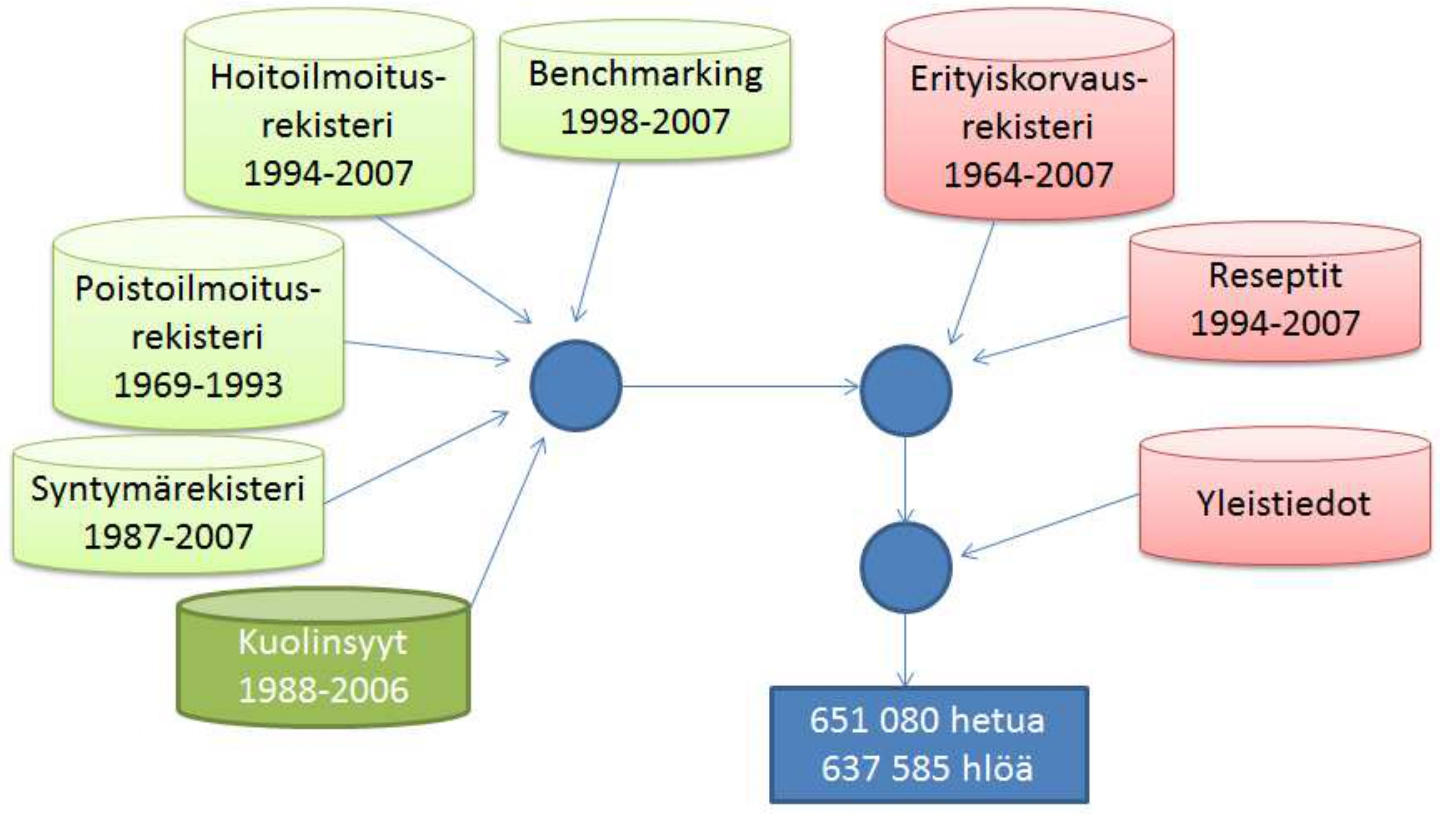
\includegraphics[width=1\linewidth]{images/diab} 

}

\caption{Vaihe 1: Diabeteskohortin identifiointi}\label{fig:diab}
\end{figure}

\FloatBarrier

\begin{eblock}{}

\textbf{Esimerkki: rekisteritutkimus pitkäaikaisen laitoshoivan käytöstä}

\begin{itemize}
\tightlist
\item
  Miten sosiaaliset tekijät, kuten sosioekonominen asema ja perherakenne, vaikuttavat laitoshoivan käyttöön?
\item
  Kolme erityistä tutkimusintressiä

  \begin{itemize}
  \tightlist
  \item
    Laitoshoivaan siirtymisen riskit
  \item
    Laitoksissa vietetty aika
  \item
    Laitoshoivan käyttö elämän loppupäässä
  \end{itemize}
\item
  Aiemmat tutkimukset samasta aiheesta

  \begin{itemize}
  \tightlist
  \item
    Perustuvat potilasaineistoihin
  \item
    Eivät sisällä laitostumis- ja poistumistietoja samassa aineistossa
  \item
    Kärsivät vastauskadosta
  \item
    Kärsivät seurantakadosta ja seurannan puutteellisuudesta
  \item
    Perustuvat pieniin aineistoihin
  \item
    Eivät mahdollista perhevaikutusten tutkimista
  \end{itemize}
\end{itemize}

\end{eblock}

\FloatBarrier

\begin{figure}

{\centering 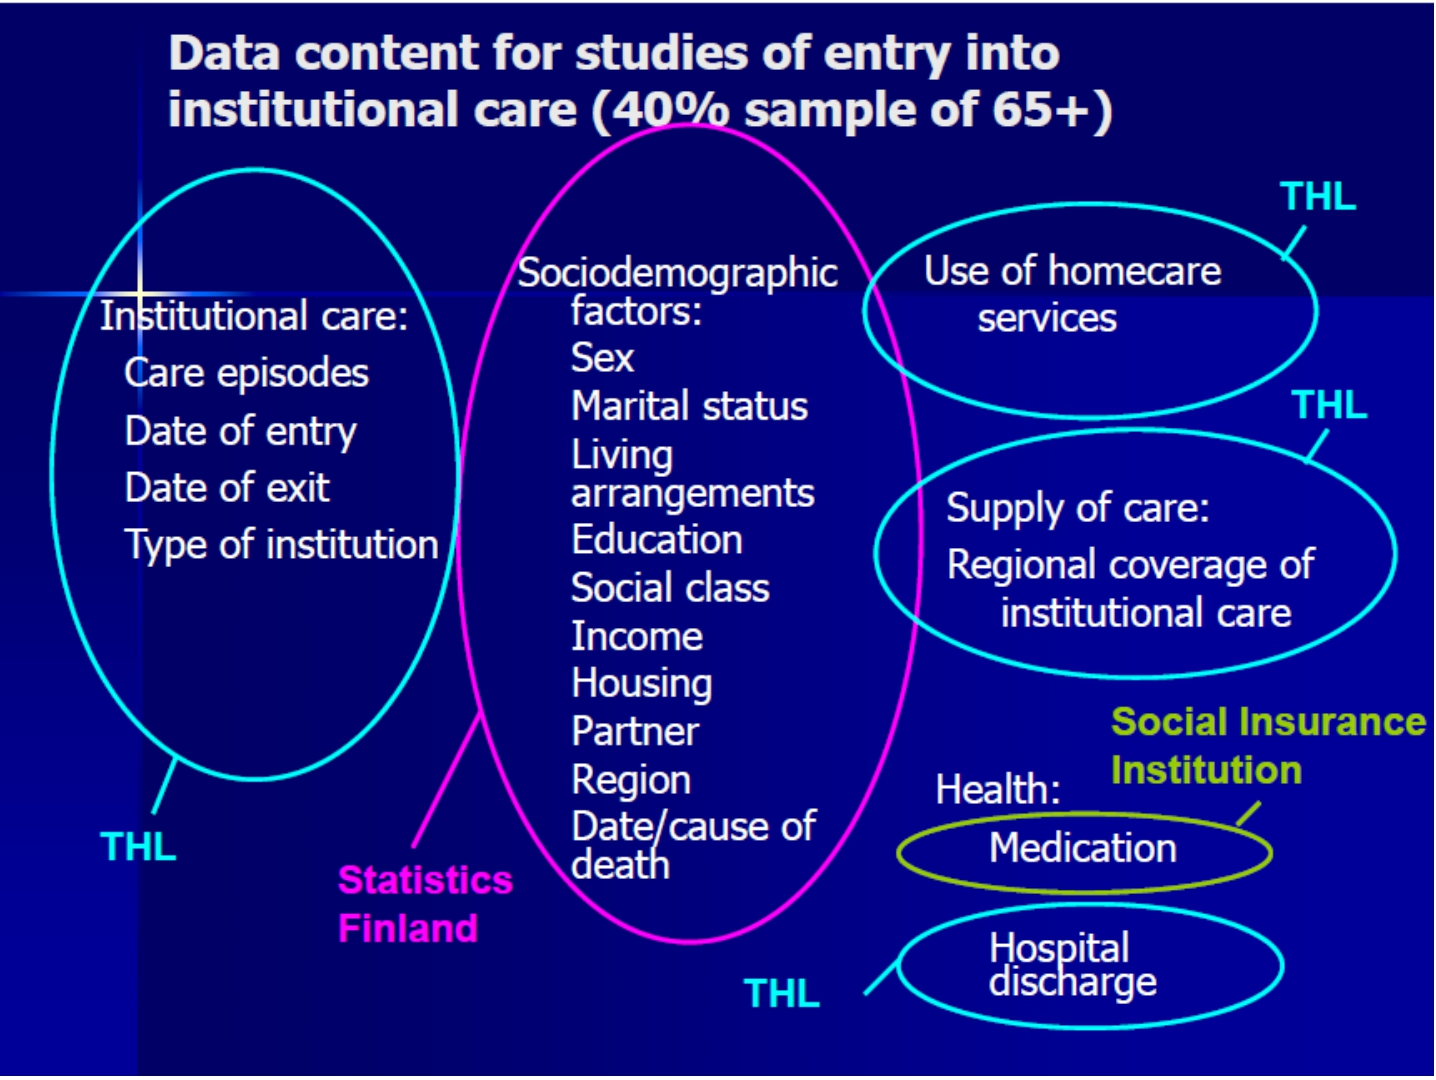
\includegraphics[width=1\linewidth]{images/rekist} 

}

\caption{Vaihe 1: Diabeteskohortin identifiointi}\label{fig:rekist}
\end{figure}

\FloatBarrier

\hypertarget{aikasarjat-ja-paneeliaineistot}{%
\subsection{Aikasarjat ja paneeliaineistot}\label{aikasarjat-ja-paneeliaineistot}}

\begin{itemize}
\tightlist
\item
  \textbf{Aikasarjat}

  \begin{itemize}
  \tightlist
  \item
    Aikasarjaksi kutsutaan havaintojen jonoa, jossa aika
    määrää jostain tilastollisesta muuttujasta tehtyjen havaintojen järjestyksen.
  \item
    Havainnot ovat tavallisesti peräkkäisiä, ja mittaukset on tehty tasaisin aikavälein, mutta väliaikojen tasaisuus ei kuitenkaan ole välttämätöntä ja monissa tutkimusasetelmissa kohdeaikasarjasta voidaan poimia havaintoja jatkuvasti tai mielivaltaisen pienin aikavälein.
  \item
    Yksittäinen aikasarja on pitkittäisaineiston erikoistapaus, jossa tarkastellaan vain yhtä aikasarjaa. Pitkittäisaineistoon nähden toistot eivät välttämättä ole suunniteltuja, vaan niitä havaitaan jatkuvasti ajassa.

    \begin{itemize}
    \tightlist
    \item
      Vuotuinen bruttokansantuote Suomessa
    \item
      Suomalaisten lukumäärä kunkin vuoden lopussa
    \item
      Vuorokautinen sademäärä Helsingin Kaisaniemessä
    \end{itemize}
  \end{itemize}
\item
  Jotkut aikasarjat ovat suunnitelmallisesti muodostettu tiettyjen laskennallisten menetelmien avulla muista aikasarjoista. Tällaisia tilastollisia suureita kutsutaan \textbf{indekseiksi} ja ne sisältävät tiivistettyä tietoa yhteiskunnasta, kuten esimerkiksi inflaation mittarina käytetty kuluttajahintaindeksi.
\end{itemize}

\begin{eblock}{}

\textbf{Esimerkki: kuluttajahintaindeksit}

\begin{itemize}
\tightlist
\item
  Hintaindeksi on normalisoitu keskiarvo tarkasteltavan tuote- tai palvelukorin hinnoista, joka lasketaan säännöllisin väliajoin tavoitteena helpottaa hintojen muutosten seurantaa eri ajankohtien tai alueiden välillä. Laajimmat indeksit mittaavat hintojen kehitystä koko talouden tasolla ja niitä hyödynnetään monin tavoin talouspolitiikassa.

  \begin{itemize}
  \tightlist
  \item
    Tilastokeskuksen haastattelijat keräävät indeksiä varten kaiken kaikkiaan noin 50 000 hintatietoa lähes 500 hyödykkeestä noin 2 700 (näin joitain vuosia sitten) liikkeestä aina kuukauden puolivälissä, lisäksi noin 1 000 hintatietoa kerätään keskitetysti.
  \item
    Tilastokeskuksen laskema kuluttajahintojen vuosimuutos oli marraskuussa 2014 oli n.~1,0 prosenttia
  \item
    Marraskuussa kuluttajahintoja nostivat viime vuodesta eniten vuokrankorotukset, tupakkatuotteiden ja alkoholijuomien vähittäishintojen ja ravintola- ja kahvilapalvelujen sekä kerrostalojen kunnossapitopalvelujen kallistuminen
  \item
    Kuluttajahintojen nousua vuoden takaisesta hillitsi marraskuussa eniten elintarvikkeiden, polttonesteiden ja viihde-elektroniikan halpeneminen
  \end{itemize}
\end{itemize}

\end{eblock}

\begin{figure}

{\centering 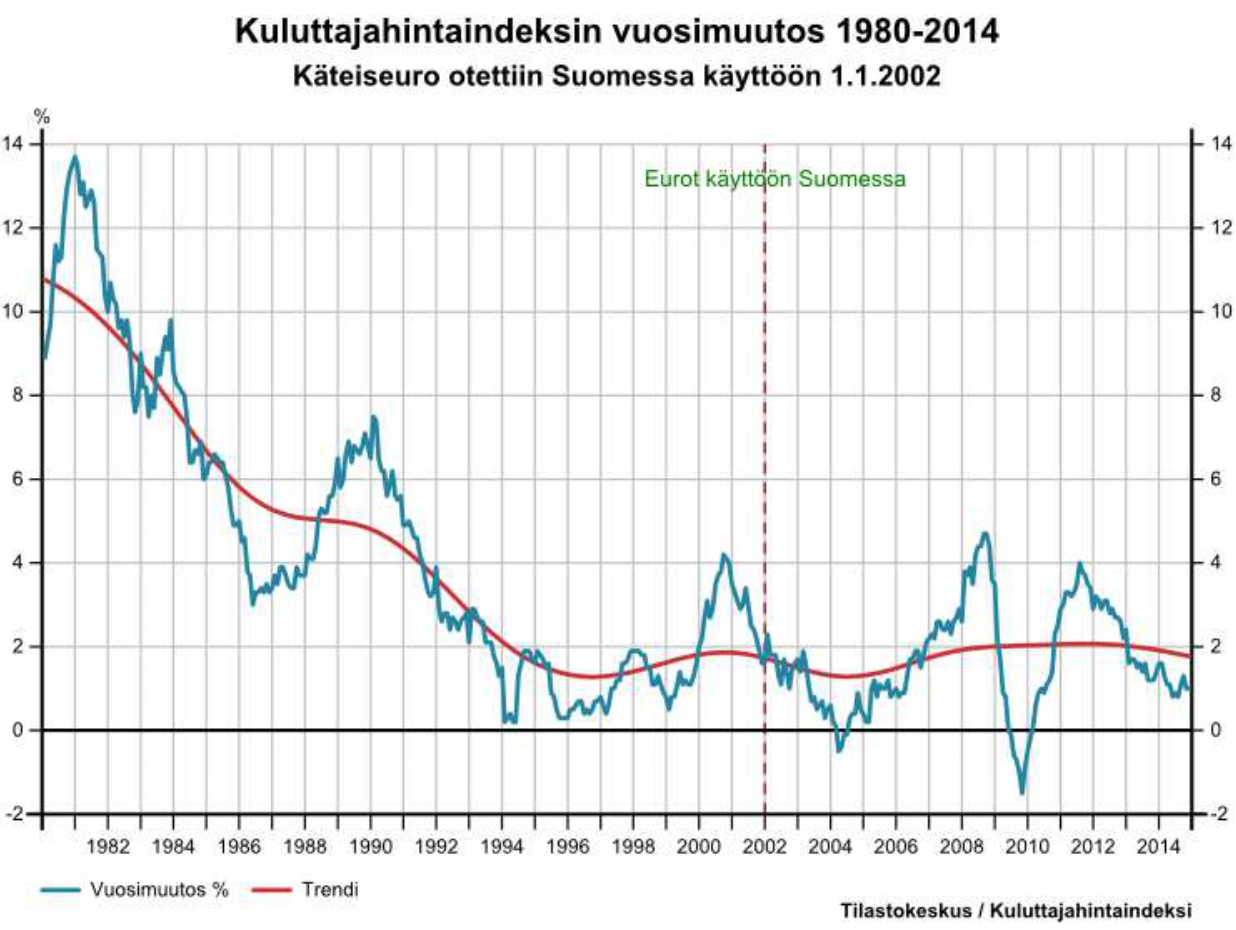
\includegraphics[width=1\linewidth]{images/kuluttaja} 

}

\caption{Esimerkki: kuluttajahintaindeksi}\label{fig:kuluttaja}
\end{figure}

\begin{itemize}
\tightlist
\item
  \textbf{Aikasarjojen tilastollinen analyysi} perustuu siihen, että sarja tulkitaan jonkin \textbf{stokastisen prosessin} eli satunnaisprosessin realisaatioksi

  \begin{itemize}
  \tightlist
  \item
    Jos aikasarjan generoinut prosessi saadaan selville, voidaan tietoja prosessista käyttää aikasarjan käyttäytymisen kuvaamiseen ja selittämiseen sekä aikasarjan tulevan käyttäytymisen ennustamiseen.
  \item
    Aikasarja-aineistot ilmentävät ilmiöstä riippuen ns. \textbf{autokorrelaatiota}, eli ajallisesti toisiaan lähellä olevat havainnot ovat korreloituneempia kuin ajallisesti kaukana toisistaan olevat.

    \begin{itemize}
    \tightlist
    \item
      Aikasarja-analyysi on yksi tilastotieteen osa-alue, jolla on rikas ja pitkälle kehittynyt teoriapohja.
    \item
      Aikasarja-analyysia opetetaan tarkemmin kursseilla \href{https://opas.peppi.utu.fi/fi/opintojakso/TILM3541/5076}{TILM3541 Aikasarja-analyysi}, \href{https://opas.peppi.utu.fi/fi/opintojakso/TILM3589/8393}{TILM3589 Epälineaarinen aikasarja-analyysi} ja \href{https://opas.peppi.utu.fi/fi/opintojakso/TILM3586/6973}{TILM3586 Moniulotteinen aikasarja-analyysi}.
    \end{itemize}
  \end{itemize}
\item
  Aikasarjoja analysoimalla voidaan selvittää esimerkiksi

  \begin{itemize}
  \tightlist
  \item
    Onko aikasarjassa \textbf{trendejä} eli aikasarjan tason systemaattisia muutoksia?
  \item
    Onko aikasarjassa \textbf{syklistä vaihtelua} kuten \textbf{suhdanne}- ja/tai \textbf{kausivaihtelua}?
  \item
    Ks. esimerkiksi kuva \ref{fig:time}.
  \end{itemize}
\end{itemize}

\FloatBarrier

\begin{figure}

{\centering 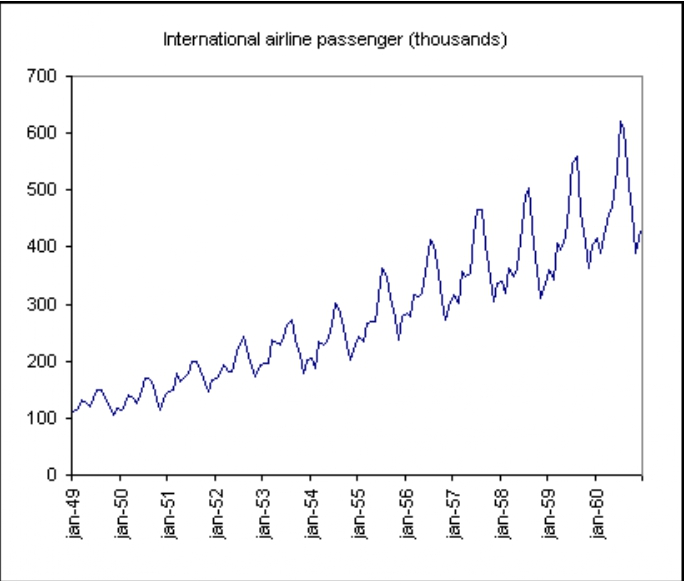
\includegraphics[width=1\linewidth]{images/time} 

}

\caption{Esimerkki: Kansainvälisten lentomatkustajien lkm vuosina 1949-1960}\label{fig:time}
\end{figure}

\hfill\break

\FloatBarrier

\begin{itemize}
\item
  \textbf{Paneeli- eli pitkittäisaineisto}

  \begin{itemize}
  \tightlist
  \item
    Paneeliaineistolla tarkoitetaan aineistoa, jossa tilastoyksiköistä on useita havaintoja ja aika määrää havaintojen järjestyksen (kuten aikasarjoissa) ja lisäksi jokaisena ajanhetkenä mitataan useampi kuin yksi tilastollinen muuttuja (kuten poikkileikkausaineistossa).

    \begin{itemize}
    \tightlist
    \item
      Paneeliaineisto on terminä käytetympi yhteiskuntatieteissä kun taas pitkittäisaineisto esimerkiksi lääketieteessä.
    \item
      Havaintoyksiköt voivat olla esimerkiksi yrityksiä, ihmisiä, kuntia tai kouluja. Ns. ``täydellisessä'' paneeliaineistossa kaikista havaintoyksiköistä on havaittu kaikki muuttujat kaikkina ajanhetkinä. ``Kiertävä'' paneeli on vastaavasti sellainen, jossa osa havaintoyksiköistä vaihtuu ajan kuluessa.

      \begin{itemize}
      \tightlist
      \item
        Tyypillisesti havaintoja kerätään tasaisin väliajoin, kuten kuukausittain tai vuosittain, ja yksittäisen ajanhetken havainto on poikkileikkausaineisto ja kustakin havaintoyksiköstä on oma usean muuttujan aikasarjansa.
      \end{itemize}
    \end{itemize}
  \item
    Paneeliaineisto mahdollistaa vastaamisen kysymykseen miksi? Yleisesti ottaen paneeliaineistoja käytetäänkin erityisesti ns. kausaalipäättelyyn tähtäävissä malleissa.\footnote{Kausaalimalleja opetetaan kurssilla \href{https://opas.peppi.utu.fi/fi/opintojakso/TILM3529/5080}{TILM3529 Kausaalipäättely havainnoivissa tutkimuksissa}}
  \end{itemize}
\end{itemize}

\hypertarget{survey--eli-haastattelu--tai-kyselytutkimus}{%
\subsection{Survey- eli haastattelu- tai kyselytutkimus}\label{survey--eli-haastattelu--tai-kyselytutkimus}}

\begin{itemize}
\tightlist
\item
  Survey-tutkimus on ei-kokeellinen tutkimus, jonka lähtökohtana on tiettyjen ilmiöiden, ominaisuuksien tai tapahtumien yleisyyden tai jakautumisen selvittäminen, joka toteutetaan kysely- tai haastattelumenetelmällä.

  \begin{itemize}
  \tightlist
  \item
    Havaintoyksiköt pyritään valitsemaan satunnaisotannalla, sillä myös survey-tutkimuksessa pyritään yleistämään tulokset otoksesta koko perusjoukkoon.
  \item
    Kyselytutkimukset muodostava kokonaan oman tutkimustapansa, joka mahdollistaa hyvin erilaisen informaation keräämisen kuin tavallisesti kvantitatiivissa aineistoissa.
  \end{itemize}
\item
  Survey-tutkimus koostuu seuraavista vaiheista:

  \begin{itemize}
  \tightlist
  \item
    Kohdepopulaation määrittely ja otannan suunnittelu
  \item
    Kyselylomakkeen rakentaminen ja testaaminen
  \item
    Kyselymetodin määrittely (puhelinhaastattelu, elektroninen kysely\ldots)
  \item
    Mahdollisten haastattelijoiden koulutus
  \item
    Aineiston keräys
  \item
    Aineiston yhteneväisyyden tarkistaminen (muuttujat tallennettu oikein jne.)
  \item
    Tulosten adjustointi mahdollisten identifioitujen virhelähteiden mukaan
  \end{itemize}
\item
  Survey-tutkimusta käytetään erityisesti asenteiden, mielipiteiden ja käyttäytymisen tutkimiseen.

  \begin{itemize}
  \tightlist
  \item
    Esimerkkejä ovat mm. poliittiset mielipidekyselyt, markkinointitutkimukset, alkoholinkulutustottumukset ja terveyspalveluiden tyytyväisyyskyselyt, joihin voi kaikkiin uskoa liittyvän vastausharhaa eri syistä.
  \item
    Esimerkiksi vastausharhaa arkaluontoisiin kysymyksiin voidaan vähentää avoimilla kysymyksillä tai alustamalla kysymystä johdannolla, jossa suvaitaan / ymmärretään kaikenlaiset vastaukset.
  \item
    ``Randomized response'': vastaukseen lisätään jonkin todennäköisyysmallin mukaisesti harhaa todellisen vastauksen salaamiseksi.
  \end{itemize}
\item
  Kerätty aineisto on siten altisteinen tehdylle kyselylle ja täten sen käyttökelpoisuus perustuu hyvin pitkälti etukäteissuunnitteluun, kunnolliseen toteutukseen ja kyselylomakkeen oikeaoppiseen rakentamiseen.

  \begin{itemize}
  \tightlist
  \item
    Lisäksi aineiston käyttökelpoisuus riippuu myös vastaajaotoksen poiminnasta (edustavuudesta) ja siitä, kuinka totuudenmukaista informaatiota vastaajat ovat kyselyssä antaneet. Tässäkin hyvä etukäteissuunnitelu on keskeistä.
  \item
    Tilastollisten menetelmien avulla pyritään arvioivaan otoksen, kyselyn suunnittelun ja kerätyn vastaajaotoksen sisältämää (tai aiheuttamaa) harhaa.
  \end{itemize}
\end{itemize}

\hypertarget{luvun-10-yhteenveto-keskeisiuxe4-termejuxe4-ja-kokonaisuuksia.}{%
\section{Luvun 10 yhteenveto, keskeisiä termejä ja kokonaisuuksia.}\label{luvun-10-yhteenveto-keskeisiuxe4-termejuxe4-ja-kokonaisuuksia.}}

\begin{itemize}
\tightlist
\item
  Kuvaileva tutkimus
\item
  Vertaileva tutkimus
\item
  Kokeellinen tutkimus
\item
  Havainnoiva tutkimus
\item
  Poikittais/poikkileikkaustutkimus
\item
  Pitkittäistutkimus (paneeli- ja pitkittäisaineistot)
\item
  Kohorttitutkimus
\item
  Tapaus-verrokkitutkimus ml. lohkot/osittaminen ja sokkouttaminen
\item
  Rekisteriaineisto
\item
  Aikasarja-aineisto
\item
  Survey eli kyselytutkimus
\end{itemize}

\hypertarget{luku11}{%
\chapter{Tilastollisesta ennustamisesta}\label{luku11}}

Kuten olemme jo tähän menneessä nähneet, tilastollinen analyysi ja sen erottamattomana osana tilastollinen päättely on keskeinen vaihe tieteellistä tutkimusta. Vielä ennen tilastollisen selittämisen ja ennustamisen välisiä eroja koskevia pohdintoja muistutetaan jo aiemmin käsitellystä \textbf{kuvailevasta tilastotieteestä}. Tämä voidaan nähdä vielä (ainakin) kolmantena yleisenä tilastotieteen tavoitteena mallintamisen/selittämisen ja ennustamisen lisäksi. Yksinkertaisin tilastollisen päättelyn muoto on hyödyntää aineistoa kuvailevia tunnuslukuja, kuten keskiarvoja ja keskihajontalukuja. Niistä voidaan kuitenkin tehdä vain melko rajoittuneita päätelmiä. Varsinkin havainnoivassa tutkimuksessa sen selvittämiseksi, miten selittävät muuttujat ovat yhteydessä selitettävään vastemuuttujaan, käytetään esim. lineaarista tai logistista regressiota (ja niiden monenmonia laajennuksia) tai esim. aikasarja-analyysiä aikasarjoja analysoitaessa. Näiden pohjalta voidaan arvioida muuttujien yhteyksiä ja riippuvuussuhteita.

Käytännössä tilastotieteen ja sen sovellusalueiden tutkimuksessa tulisi osata erottaa (tilastollinen) \textbf{selittäminen} ja \textbf{ennustaminen}. Tätä eroa koskevat tarkemmat yksityiskohdat ovat jälleen selvästi tämän kurssin ulkopuolella myöhemmissä tilastotieteen opinnoissa, mutta seuraavassa kuitenkin tähän liittyviä keskeisiä huomioita.

\hypertarget{alaluku111}{%
\section{Tilastollinen selittäminen vs.~ennustaminen}\label{alaluku111}}

\begin{itemize}
\tightlist
\item
  (Tilastollinen) \textbf{selittäminen} tarkoittaa esim. kahden muuttujan välisen yhteyden tutkimista (tämän kurssin yksinkertainen tilanne lineaarisen regressiomallin yhteydessä, jota voidaan laajentaa useisiin muuttujiin). Tutkijaa saattaa kiinnostaa esimerkiksi tupakoinnin vaikutus sepelvaltimotautikuolleisuuteen tai ylipainon vaikutus leikkauksen jälkeisiin infektioihin.

  \begin{itemize}
  \tightlist
  \item
    Tällöin \textbf{pyrkimyksenä} on rakentaa ``\textbf{selitysmalli}'', jossa on perustellut syy-seuraussuhteet selittävästä (selittävistä) muuttujista selitettävään muuttujaan.
  \end{itemize}
\item
  (Tilastollinen) \textbf{ennustaminen} tarkoittaa, että tietyillä selittävän tai selittävien (tai ``ennustavien'') muuttujien yhdistelmillä voidaan ennustaa ennustettavan muuttujan arvoa.

  \begin{itemize}
  \tightlist
  \item
    Ts. siis ennustettavana muuttujana toimii tilastollisen mallin näkökulmasta katsoen vastemuuttujan arvo, jota pyritään ennustemallin avulla ennustamaan.
  \item
    Ennustemalleja tutkittaessa varsinaisilla selityssuhteilla ei välttämättä ole merkitystä. Tärkeintä on mallin ennustekyky, ei niinkään esim. yksittäisen regressiokertoimen arvo ja siihen liittyvät tarkemmat tulkinnat. Tilastollisesti merkitsevä regressiokerroin ei tarkoita, että muuttujalla olisi välttämättä ennustekykyä.
  \item
    Ennustekyky tutkittava erikseen. Esimerkiksi lineaarisen mallin perinteiset tunnusluvut, kuten selitysaste, eivät vielä kerro mallin todellisesta ennustekyvystä paljoakaan. Tästä huolimatta melko usein ennustemallin rakentaminen perustetaan pitkälle samoihin tilastollisen päättelyn ja estimointiteorian lähtökohtiin mitä olemme jo sivunneet tällä kurssilla.
  \item
    Hyvin usein tutkimuksissa raportoidaan, että tietty muuttuja ``ennustaa'' (predicts) toista. Usein kuitenkin taustalla on tällöin usean muuttujan selitysmalli, jonka regressiokertoimien tilastollista merkitsevyyttä on tulkittu. Yleensä tässä yhteydessä on kuitenkin siis kyse selittämisestä, ja kuten todettua, mallin ennustekyky pitää tutkia erikseen.
  \end{itemize}
\item
  Erityisesti aikasarja-analyysissä ennustaminen on perinteisesti ollut yksi kaikkein keskeisimmistä tavoitteista.

  \begin{itemize}
  \tightlist
  \item
    Nyt kuitenkin \textbf{koneoppimisen (tilastollisen oppimisen)} kasvatettua hurjasti suosioitaan viime vuosina ennustaminen on levinnyt, ja leviää jatkossakin, voimakkaasti myös hyvin keskeiseksi osaksi muutakin tilastollista analyysiä.
  \end{itemize}
\end{itemize}

\hypertarget{alaluku112}{%
\section{Tilastolliseen ennustamiseen liittyviä huomioita}\label{alaluku112}}

\begin{itemize}
\item
  Ennustamista on kaikkialla! Sen rooli on paljon keskeisempi osa meidän kaikkien arkea mitä ensiajatukselta saattaa tulla mieleen.

  \begin{itemize}
  \tightlist
  \item
    Ennustaminen on elämässämme korvaamatonta.\footnote{Tämän alaluvun pohdinnat, kuten tämä lainaus, perustuvat pitkälle Silverin kirjan Signaali ja kohina (suom. Kimmo Pietiläinen) huomioihin.}
  \item
    Kun valitsemme reitin työmatkalle, päätämmekö menemmekö toisille treffeille tai säästämme huonompia aikoja varten, teemme ennusteen tulevaisuuden kehityksestä ja siitä, miten suunnitelmamme vaikuttavat suotuisan tuloksen todennäköisyyteen.
  \end{itemize}
\item
  Arkiset ongelmat eivät aina vaadi ankaraa ajattelua ja pohdiskelua erilaisten vaihtoehtojen välillä niihin käytettävissä olevan ajan ollessa rajallinen. Tästä huolimatta teet ennusteita tiedostaen ja useimmiten tiedostamatta monta kertaa päivässä!
\item
  \textbf{Ennustevirhe}:

  \begin{itemize}
  \tightlist
  \item
    Ennusteita verrataan toteutuneeseen kehitykseen. Näiden erotuksena muodostuu ennustevirhe.
  \item
    Lähtökohtana on (luonnollisesti) minimoida ennustevirheet. Käytännössä useinmiten mm. vastemuuttujan luonteen perusteella valitaan sopiva ennustevirheitä summarisoiva tunnusluku, kuten keskineliöennustevirhe (jatkuvat vastemuuttujat) tai luokitteluvasteiden tapauksessa väärin (tai oikein) ennustettujen luokitteluiden suhteellinen osuus.
  \item
    Ajoittain ennustetarkkuutta on helpompi ja toisaalta sitten vaikeampi tarkkailla. Esim. taloustieteessä on paljon helpompi arvioida työttömyyttä koskevaa ennustetta kuin esimerkiksi ennustetta (jopa väitettä) velkaelvytyksen tehokkuudesta. Toisaalta valtio-opissa voidaan arvioida vaalitulosta koskevia ennusteita suoraviivaisesti, mutta saattaa kulua vuosikymmeniä nähdä miten poliittisten instituutioiden ennusteisiin perustuvat ennakoidut muutokset vaikuttavat poliittisten päätösten tuloksiin.
  \end{itemize}
\end{itemize}

\begin{eblock}{}

\textbf{Esimerkki: Silverin kirjan luvun 1 pohdintaa ennustevirheestä \emph{finanssikriisiin} (\emph{rahoituskriisiin}) vuoden 2008 aikana (finanssikriisin voidaan katsoa koskeneen lopulta vuosia 2007-2009).}

Pörssikurssien voimakas lasku, Lehman Brothersin kaltaisia aikoinaan arvostettuja yhtiöitä meni vararikkoon, luottomarkkinat olivat käytännössä ``jäätyneet'', Las Vegasissa asuntojen hinnat laskivat 40 prosenttia (osoittaen osaltaan vallinnutta laajempaakin ``\textbf{asuntokuplaa}'' (perusteettoman korkeita asuntojen hintoja), työttömyys kasvoi räjähdysmäisesti jne.

\hfill\break

\textbf{Ennustevirheen yhteisiä ja tyypillisiä piirteitä} (tässä tapauksessa), jotka laajentuvat moniin muihinkin tilanteisiin ja sovelluksiin:

\begin{enumerate}
\def\labelenumi{\arabic{enumi}.}
\tightlist
\item
  Asunnonomistajat ja sijoittajat ajattelivat, että nousevat hinnat viittasivat siihen, että asuntojen hinnat jatkaisivat nousuaan, kun todellisuudessa historia viittasi siihen, että sen takia niillä oli taipumus laskea (näissä olosuhteissa).
\item
  Luottoluokistuslaitokset (samoin kuin Lehman Brothersin kaltaiset pankit) eivät ymmärtäneet, miten riskialtiita asuntovakuudelliset arvopaperit olivat. Ongelma ei varsinaisesti ollut siinä, että luokituslaitokset eivät nähneet asuntokuplaa. Sen sijaan niiden ennustemallit olivat täynnä huonoja oletuksia ja väärää ``itseluottamusta'' mahdollisten asuntojen hintojen romahduksen riskeistä.
\item
  Laajasti ei ennakoitu, miten asuntokriisi laukaisee globaalin rahoituskriisin. Se johtui suurelta osin liiallisesta velkaantumisesta markkinoilla, jossa lyötiin erinäisten instrumenttien myötä vetoa yhdysvaltalaisten halukkuuden puolesta sijoittaa uuteen kotiin.
\item
  Rahoituskriisin välittömissä jälkimainingeissa ei osattu ennustaa, miten laajoja taloudellisia ongelmia se aiheuttaa. Rahoituskriisit tyypillisesti tuottavat erittäin syviä ja pitkäkestoisia taloudellisia taantumajaksoja.
\end{enumerate}

Näissä ennustamisen epäonnistumisissa on \textbf{yhteinen piirre}. Kussakin tapauksessa aineistoa arvioidessaan ihmiset jättivät keskeisen asiayhteyden palan huomiotta:

\begin{enumerate}
\def\labelenumi{\arabic{enumi}.}
\tightlist
\item
  Asunnonomistajien luottamus asuntojen hintoihin johtui ehkä siitä, että lähimenneisyydessä Yhdysvalloissa asuntojen hinnat eivät olleet laskeneet merkittävästi. \textbf{\emph{Kuitenkaan}} koskaan aikaisemmin Yhdysvaltojen asuntojen hinnat eivät olleet nousseet niin laajalla alueella kuin romahdusta edeltävällä kaudella.
\item
  Pankkien luottamus luottoluokituslaitosten (kuten Moody'siin ja S\&P'siin) kykyyn luokittaa asuntovakuudellisia arvopapereita ehkä perustui siihen, että laitoksina ne olivat onnistuneet pätevästi luokittamaan muunlaista rahoitusomaisuutta. \textbf{\emph{Kuitenkaan}} luottoluokituslaitokset eivät olleet koskaan aikaisemmin luokittaneet yhtä uusia ja monimutkaisia arvopapereita mitä tuolloin (kuten ns. luotonvaihto-optioita).
\item
  (Taloustietelijöiden) luottamus rahoitusjärjestelmän kykyyn kestää asuntokriisi syntyi ehkä siitä, että aikaisemmin asuntojen hintojen heilahtelulla ei yleensä ollut suuria vaikutuksia rahoitusjärjestelmässä. \textbf{\emph{Kuitenkaan}} rahoitusjärjestelmä ei luultavasti koskaan aikaisemmin ole ollut yhtä vekkaantunut eikä vedonlyöntiä asuntojen hinnoista ollut tehty vastaavassa mittaluokassa.
\item
  Poliittisten päättäjien luottamus siihen, että talous toipuu nopeasti rahoituskriiseistä syntyi ehkä viime vuosikymmenten taantumista saaduista kokemuksista. Useampia niitä oli seurannut nopea ``V-muotoinen'\,' toipuminen (kuten nyt myös myöhemmin mm. koronapandemian aikaan). \textbf{\emph{Kuitenkaan}} nämä taantumat eivät olleet liittyneet rahoituskriiseihin ja rahoituskriisit ovat (yleensä) erilaisia.
\end{enumerate}

Jokaista edellistä kohtaa yhdistää ennustamiseen hyvin keskeisesti liittyvä termi: Ennustajien pohtimat ilmiöt olivat ns. \textbf{otoksen ulkopuolella} (engl. \textbf{out-of-sample}). Kun ennustaminen epäonnistuu merkittävällä tavalla, tämä ongelma jättää yleensä runsaasti sormenjälkiä rikospaikalle. Miten tämä ongelma näyttäytyy siis oheisen esimerkin tapauksessa?

\begin{itemize}
\tightlist
\item
  Luottoluokituslaitos (kuten Moody's) arvioi, missä määrin asuntolainojen hoitamatta jättämiset liittyivät toisiinsa, rakentamalla (luultavasti ainakin osin) tilastollisen mallin menneisyyden aineiston perusteella. Oletettavasti he käyttivät mallin rakentamiseen noin 1980-luvulle ulottuvaa Yhdysvaltain asuntomarkkina-aineistoa.
\item
  Ongelmana oli, että 1980-luvulta 2000-luvun alkuvuosiin saakka asuntojen hinnat olivat aina vakaat tai nousevat Yhdysvalloissa. Tässä tilanteessa oletus, että asunnonomistajien asuntolainat eivät juurikaan liittyneet toisiinsa oli luultavasti perusteltu ja riittävän hyvä tilastollisen mallintamisen pohjaksi.
\item
  Kuitenkaan menneessä aineistossa mikään ei olisi kuvannut mitä tapahtuu kun asuntojen hinnat alkavat laskea kauttaaltaan samanaikaisesti. Ts. asuntoromahdus oli \textbf{otoksen ulkopuolinen tapahtuma} ja tässä tilanteessa luottoluokituslaitosten mallit olivat arvottomia (huonoja) lainojen hoitamatta jättämisen riskiä arvioitaessa.
\end{itemize}

\end{eblock}

\hfill\break

\begin{itemize}
\tightlist
\item
  Rahoituskriisiä koskevan esimerkin tilanteessa otoksen ulkopuolisiä ilmiöitä koskeva ongelma realisoitui siten, että muodostettu tilastollinen malli, kuten vaikkapa lineaarisen regressiomallin sopiva laajennus, \textbf{estimoitiin}, tai koneoppimisesta tutussa kielenkäytössä \textbf{opetettiin}, aineistolla, joka ei lopulta ollut relevantti juuri myöhemmin tapahtunutta kriisivaihetta ajatellen.

  \begin{itemize}
  \tightlist
  \item
    Onkin tärkeää ymmärtää, että ``todellisessa'' ennustetilanteessa joudumme käyttämään aiempaa aineistoa mallien ja algoritmien rakentamiseen. Näin ollen näiden ennustekykyä arvioitaessa onkin mentävä otoksen ulkopuolelle, koska ``otoksen sisällä'' voimme opettaa kyseisiä malleja (ääritilanteessa) niin, että ne ovat periaatteessa äärettömän tarkkoja. Ne eivät kuitenkaan takaa missään mielessä hyvää ennustekykyä tulevia tapahtumia ennustettaessa.
  \end{itemize}
\item
  Vastaavalla tavalla karakterisoidaan nykyään hyvin suosittujen koneoppimismenetelmien keskeinen piirre: ne ja tarkasteltavat sovellukset perustuvat käytännössä (vielä) lähes yksinomaan ennustesovelluksiin. Tällöin mallien ja algoritmien opettaminen ns. \textbf{opetusaineistolla} (edellä olevassa esimerkissä aiemmalla asuntomarkkina-aineistolla) ja ennustekyvyn arviointi \textbf{ennusteotoksen} avulla pitää erottaa toisistaan.

  \begin{itemize}
  \tightlist
  \item
    \textbf{Otoksen sisäiseen sovittamiseen} (engl. \textbf{in-sample} tai \textbf{training sample} estimation, ajoittain prediction) liittyy siis (ennustamisen näkökulmasta) katsoen ns. \textbf{ylisovittamisen} vaara. On mahdollista, että yritämme puristaa lähes puhtaasta kohinasta signaaleja, jotka eivät missään mielessä tule olemaan valideja otoksen ulkopuolisessa ennustamistilanteessa.
  \item
    Jälleen kerran näistä teemoista keskustellaan tarkemmin myöhemmin tilastotieteen aine- ja syventävien opintojen erikoiskursseilla, kuten \href{https://opas.peppi.utu.fi/fi/opintojakso/TILM3587/6975}{TILM3587 Regressioanalyysi ja tilastollinen oppiminen} ja \href{https://opas.peppi.utu.fi/fi/opintojakso/TILM3592/13413}{TILM3592 Tilastollisen oppimisen jatkokurssi}.
  \end{itemize}
\item
  Huolimatta edellä käydystä, kriittisestäkin, keskustelusta ennustamiseen liittyen, monet ennusteet ovat varsin tarkkoja ja samalla vapaita ylisovittamisen vaaroista!
\end{itemize}

\hypertarget{luvun-11-yhteenveto-keskeisiuxe4-termejuxe4-ja-kokonaisuuksia.}{%
\section{Luvun 11 yhteenveto, keskeisiä termejä ja kokonaisuuksia.}\label{luvun-11-yhteenveto-keskeisiuxe4-termejuxe4-ja-kokonaisuuksia.}}

\begin{itemize}
\tightlist
\item
  Tilastollinen ennustaminen
\item
  Selitysmalli vs.~ennustemalli
\item
  Ennuste ja ennustevirhe
\item
  Opetusaineisto vs.~ennusteotos
\item
  In-sample/training sample vs.~out-of-sample (forecasting)
\end{itemize}

\hypertarget{luku12}{%
\chapter{Tilastotieteen kehityksen nykytrendejä}\label{luku12}}

\hypertarget{modernin-tilastotieteen-suuntaviivoja}{%
\section{Modernin tilastotieteen suuntaviivoja}\label{modernin-tilastotieteen-suuntaviivoja}}

Seuraavassa vielä joitain tilastotiedettä parhaillaan koskevia kehitystrendejä, joita olemme myös osaltaan sivunneet tämän kurssimateriaalin myötä:

\begin{itemize}
\item
  \textbf{Aineistot kasvavat ja monimutkaistuvat}. Näin ollen tilastotietedettä ja tilastollisten menetelmien kehitystyötä tullaan tarvitsemaan (yhä suuremmin) jatkossakin.
\item
  Informaatiota on tarjolla (paljon) enemmän kuin osaamme sitä hyödyntää. \textbf{Informaatio ei ole enää niukka hyödyke}. Keskeistä on kuitenkin, että (useimmiten) suhteellisen pieni osa informaatiosta on hyödyllistä.

  \begin{itemize}
  \tightlist
  \item
    Havaitsemme informaatiota (osin) ja valikoivasti subjektiivisesti. Luulemme haluavamme lisää informaatiota, kun todellisuudessa haluamme tietoa (ts. signaaleja kun vastaavasti kasvava määrä kohinaa yrittää vaikeuttaa tätä signaalin erottamista kohinasta).
  \end{itemize}
\item
  \textbf{Laskennallisuus} kasvaa. Tietokoneiden laskentakapasiteetti nousee vaikkakin suhteellinen kasvu ei ehkä olekaan enää niin suurta mitä muutamat viime vuosikymmenet.
\item
  Osin laskennallisuuteen liittyvä \textbf{koneoppimisen} kehittyminen ja sen ``rajatieteiden'' yhteyteen integroituneet käytännöt ja menetelmäkehitystyö tulee jatkumaan.

  \begin{itemize}
  \tightlist
  \item
    Toisaalta ``perinteiselle'' tilastotieteelle on edelleen myöskin vahva oma roolinsa monilla eri tieteenaloilla.
  \end{itemize}
\item
  \textbf{Analyysien automatisointi}: Tilastolliset ohjelmat alkanevat jatkossa tulkita tuloksia osin automaattisesti. Mihin tarvitaan tilastotieteilijää? Kokonaisvaltaiseen tutkimusprosessin valvontaan(?)

  \begin{itemize}
  \tightlist
  \item
    Osin edelliseen liittyen jo nyt ja jatkossa luultavasti yhä enemmän korostuu se, että melkein kuka vaan voi tehdä tilastollisia analyysejä. Niin valmiita paketteja jne. on jo saatavilla. ``Tilastotieteellinen faktantsekkaus'' noussee vahvemmin esille eli tilastollisten menetelmien käyttäjän on sittenkin edelleen kyettävät arvioimaan ovatko tulokset uskottavia ja vapaita ilmeisistä hankaluuksista.
  \item
    Näiltä osin yksi keskeinen kehityssuunta on jo vahvasti yleistyneet laajat tekoälymallit kuten OpenAI:n toteuttama \href{https://chat.openai.com/}{ChatGPT}.

    \begin{itemize}
    \tightlist
    \item
      ChatGPT:tä käytetäänkin jo laajalti mm. tilastollisen ohjelmoinnin apuvälineenä. Nopeasta kehityksestä huolimatta ChatGPT:n antamat vastaukset ovat kuitenkin paikoin epäluotettavia tai suorastaan väärin, joten sen käytössä korostaa edelleen vahvan tilastotieteellisen osaamisen lisäksi substanssiosaaminen.
    \end{itemize}
  \end{itemize}
\item
  \textbf{Poikkitieteellisyys} tulee entisestäänkin vahvistumaan. Ts. substanttitietouden ja tilastotieteen yhdistäminen ja sen tärkeys ei tule ainakaan vähenemään. Sivuaineopintoja kannattaa siis käydä ja ottaa opinto-ohjelmaan.

  \begin{itemize}
  \tightlist
  \item
    Tämän lisäksi kokonaisvaltaisesti tilastotieteen ytimen osaajien osaamista tulla kysymään jatkossakin.
  \end{itemize}
\end{itemize}

\hfill\break

\begin{itemize}
\tightlist
\item
  Oheisten huomioiden ohella lopuksi on syytä korostaa tilastotieteen opiskelun näkökulmasta, että oikotietä ei ole! \textbf{Oikaista siis ei voi}: Ensin on rakennettava vahva tilastollisen ajattelun ja menetelmien perusta (\textbf{alkaen todennäköisyyslaskennasta ja tilastollisesta päättelystä}), jotta myöhemmin voi kehittyä ja omata todellisia kykyjä ottaa vastaan monia jo varsin monimutkaisia tilastollisia menetelmiä!
\end{itemize}

\hypertarget{luvun-12-yhteenveto-keskeisiuxe4-termejuxe4-ja-kokonaisuuksia.}{%
\section{Luvun 12 yhteenveto, keskeisiä termejä ja kokonaisuuksia.}\label{luvun-12-yhteenveto-keskeisiuxe4-termejuxe4-ja-kokonaisuuksia.}}

\begin{itemize}
\tightlist
\item
  Aineistot kasvavat ja monimutkaistuvat
\item
  Informaatio ei ole enää niukkaa
\item
  Laskennallisuus kasvaa
\item
  Koneoppimisen vahvistuminen ja kehittyminen
\item
  Analyysien automatisoituminen
\item
  Poikkitieteellisyys
\end{itemize}

  \bibliography{book.bib,packages.bib}

\end{document}
